\documentclass[a4 paper, 12pt]{article}
\usepackage{fullpage}
\usepackage{textcomp}
\usepackage[font={small,it}]{caption}
\usepackage{endnotes}

\makeatletter
\def\enoteheading{\section*{\@mkboth{\MakeUppercase{\notesname}}{\MakeUppercase{\notesname}}}%
  \mbox{}\par\vskip-0\baselineskip\noindent\rule{.5\textwidth}{0.4pt}\par\vskip-0\baselineskip}
\makeatother
\usepackage{enumitem}
\usepackage{float}
\usepackage{fontspec}
\usepackage{titlesec}
\newfontfamily{\sectionfont}[Ligatures=TeX]{Arial}
\titleformat*{\section}{\sectionfont\LARGE}
\titleformat*{\subsection}{\sectionfont\Large}
\titleformat*{\subsubsection}{\sectionfont\large}
\setmainfont[Ligatures=TeX]{Times New Roman}
\makeatletter
\renewcommand\@makefntext[1]{%
\noindent\makebox[0em][r]{\@makefnmark}#1}
\makeatother
\usepackage{xfrac}
\usepackage{xcolor}
\usepackage[hidelinks]{hyperref}
\hypersetup{pdfauthor={rob.abhidhamma@gmail.com}, pdfsubject={Abhidhamma}, pdftitle={Practical Abhidhamma Course}}
\hypersetup{colorlinks=true, linkcolor=black, urlcolor=blue}
\usepackage{multicol}
\newcommand{\hpadright}[1]{#1 \hspace{2mm}}
\newcommand{\question}[1]{\subsubsection*{#1}}
\usepackage{quoting}
\quotingsetup{vskip=0pt}
\usepackage{wasysym}
\newcommand{\tmcommon}{\hspace{2.5mm}\CIRCLE}
\newcommand{\tm}{\hspace{2.5mm}\Circle}
\usepackage{booktabs}
\usepackage{multicol}
\usepackage{multirow}
\usepackage{array}
\newcolumntype{L}[1]{>{\raggedright\let\newline\\\arraybackslash\hspace{0pt}}m{#1}}
\newcolumntype{C}[1]{>{\centering\let\newline\\\arraybackslash\hspace{0pt}}m{#1}}
\newcolumntype{R}[1]{>{\raggedleft\let\newline\\\arraybackslash\hspace{0pt}}m{#1}}
\newcommand{\tableheader}[1]{{\sectionfont \textbf{#1}}}
\newcommand{\tablesubheader}[1]{{\sectionfont #1}}
\newcommand{\tablevsubheader}[1]{\hspace{2.5mm}\rotatebox[origin=l]{90}{\tablesubheader{#1}\hspace{1mm}}}
\newcommand{\tablevsubheaderhack}[1]{\hspace{2mm}\rotatebox[origin=l]{90}{\tablesubheader{#1}\hspace{1mm}}}
\usepackage{subcaption}

\title{Practical Abhidhamma Course\\{\normalsize \textbf{\textit{Version 1.0 (February 2016)}}}}
\author{}
\date{}
\hyphenation{abhi-dhamma Mahā-vihāra Ti-piṭaka Buddha-ghosa Visuddhi-magga}
 
\begin{document}

%\maketitle

\begin{center}
\includegraphics[width=0.5\linewidth]{./Diagrams/Front}
\end{center}

\tableofcontents
%\begin{center}
\textbf{\textit{Namo Tassa Bhagavato Arahato Sammā Sambuddhassa}} \\
\end{center}

This course is for Theravāda\footnote{\url{http://en.wikipedia.org/wiki/Theravada}} Buddhists with inquiring minds who want an introduction\footnote{Additional details can be found in the following texts (these texts are referenced in footnotes):\\
“\textbf{A Comprehensive Manual of Abhidhamma}” (\textit{Abhidhammattha Sangaha}) Bhikkhu Bodhi (\url{http://store.pariyatti.org/Comprehensive-Manual-of-Abhidhamma-A--PDF-eBook_p_4362.html})\\
“\textbf{Path of Purification}” (\textit{Visuddhimagga}) Bhikkhu Ñāṇamoli (\url{http://www.accesstoinsight.org/lib/authors/nanamoli/PathofPurification2011.pdf})\\
“\textbf{Buddhist Dictionary}” Nyanatiloka (Ñāṇatiloka) (\url{http://urbandharma.org/pdf/palidict.pdf})\\
“\textbf{Cetasikas}” Nina van Gorkom (\url{http://archive.org/details/Cetasikas})\\
“\textbf{The Buddhist Teaching on Physical Phenomena}” Nina van Gorkom (\url{http://archive.org/details/TheBuddhistTeachingOnPhysicalPhenomena})\\
“\textbf{The Conditionality of Life (Outline of the 24 conditions as taught in the Abhidhamma)}” Nina van Gorkom (\url{http://archive.org/details/TheConditionalityOfLife})\\
When publications of the Pali Text Society are referenced, page numbers refer to the English translation.} to the Abhidhamma with minimal Pāḷi.\footnote{\url{http://en.wikipedia.org/wiki/Pali}} It includes audio recordings of eight talks, handouts to accompany the talks and a document. The recordings, handouts and the document can be downloaded from \url{http://practicalabhidhamma.com/}.

Some people may prefer listening to the recordings with the handouts in front of them.\footnote{When listening to the talks for the first time, you may have an impression of “information overload”, like trying to take a drink from a fire hose! \smiley \ If so, you may want to listen to the talks a second time or read the document.} Others may find they absorb more by reading the transcript of the talks in the document with the handouts in front of them. The document includes many diagrams and footnotes with links to online resources such as Suttas, stories from the Dhammapada Commentary and Wikipedia articles.\footnote{The footnotes are not merely an academic convention, they are my invitation to you to explore further. When viewing this document on a laptop or a tablet, the links are active; clicking a link shows the online website.} The document also includes Questions \& Answers for each talk. 

The talks cover selected topics from the Abhidhamma that are most practical and relevant to daily life. Though it is called a “Practical Abhidhamma Course,” it is also a practical Dhamma\footnote{In this context, “Dhamma” (\url{http://en.wikipedia.org/wiki/Dharma}) means both the Buddha’s teachings (capitalized “Dhamma”) and the Ultimate Realities of the Abhidhamma (lower case “dhamma”).} course using themes from the Abhidhamma.

The Dhamma and the Abhidhamma are \textbf{not} meant for abstract theorizing; the Dhamma and the Abhidhamma are meant for practical application. I hope you approach this course not only to learn new facts, but also to consider how you can improve yourself spiritually.\footnote{The Commentary speaks of a progression: study (\textit{pariyatti}), practice (\textit{paṭipatti}) and realization (\textit{paṭivedha}).}

\subsubsection*{Acknowledgements}

Ayyā Medhānandī Bhikkhunī suggested that I prepare this Practical Abhidhamma Course after a talk I gave at Sati Sārāṇīya Hermitage (\url{http://satisaraniya.ca/}). I am very grateful to the Venerables who reviewed the draft and corrected inaccuracies. Many of the questions came from my friends/students. Oli Cosgrove proofread the document and improved the writing style. My son Dion helped with aesthetics and all things digital (\LaTeX, audio and webpage).

\section{Introduction}

Welcome to this Practical Abhidhamma Course. This first lesson provides context by introducing the Abhidhamma as part of the Buddhist canon.

\subsection*{Structure of the Buddhist canon}

\begin{figure}[H]
\centering
\input{./Diagrams/Tipitaka.pdf_tex}
\caption{The Tipiṭaka consists of three collections: Vinaya, Suttas and Abhidhamma.}
\label{fig:Tipitaka}
\end{figure}

Let’s start by looking at the “Structure of the Buddhist Canon” diagram in Figure \ref{fig:Tipitaka}.

\textit{Tipiṭaka} is a Pāḷi word; in Pāḷi, \textit{Ti} means three and \textit{Piṭaka} means basket, so \textit{Tipiṭaka} is literally “three baskets” meaning “three collections.”\footnote{\url{http://en.wikipedia.org/wiki/Tipitaka}} The first collection is the Vinaya, the rules for monks and nuns. The second collection is the Suttas, the spoken discourses given by the Buddha and his disciples using conventional language. The third collection is the Abhidhamma; it provides a detailed framework covering all the teachings. \textit{Abhi} is a Pāḷi prefix meaning “higher” and so Abhidhamma literally means higher teachings.\footnote{In “The Expositor” (\textit{Atthasālinī}) page 3, Buddhaghosa explains that the prefix “\textit{Abhi}” also indicates that the Abhidhamma “exceeds and is distinguished from the Dhamma (the Suttas).”}

Let me help you to visualize the size of the \textit{Tipiṭaka}.\footnote{In the world’s largest book (\url{http://en.wikipedia.org/wiki/World’s_largest_book}), the entire \textit{Tipiṭaka} is written in Pāḷi using Burmese script on the front and back of 729 marble slabs (total of 1458 “pages”); 222 “pages” of Vinaya, 820 “pages” of Suttas and 416 “pages” of Abhidhamma.} The printed \textit{Tipiṭaka} fills a bookshelf one metre in length. The Suttas make up about half of the \textit{Tipiṭaka}, the Abhidhamma makes up about one third of the \textit{Tipiṭaka} and the Vinaya makes up about one sixth of the \textit{Tipiṭaka}.\footnote{Each of the books in the Vinaya, Suttas and Abhidhamma have Commentaries (\textit{Aṭṭhakathā}: \url{http://en.wikipedia.org/wiki/Atthakatha}) and many have Subcommentaries (\textit{Ṭīkā}: \url{http://en.wikipedia.org/wiki/Subcommentaries,_Theravada}). The Commentaries were compiled about 1500 years after the Buddha's \textit{parinibbāna} (this is discussed in the next lesson) and the Subcommentaries were prepared later. Most of the Commentaries and Subcommentaries have not been translated into English. A Pāḷi version of the \textit{Tipiṭaka}, Commentaries and Subcommentaries can be downloaded from the Vipassana Research Institute site: \url{http://www.tipitaka.org/cst4}}

\pagebreak

Over the past 60 years, 11 monks in Myanmar have memorized the entire \textit{Tipiṭaka}.\footnote{These monks are given the title “\textit{Tipiṭaka dhara}”: \url {http://www.myanmarnet.net/nibbana/tipitaka/tpdkdhra.htm}} The first of these monks got into the Guinness Book of Records for reciting 16,000 pages of the \textit{Tipiṭaka}.\footnote{\url{http://en.wikipedia.org/wiki/Mingun_Sayadaw}} Amazing! I have become so dependent on technology that sometimes I can’t even remember my wife’s phone number!

\subsection*{Vinaya}

The first part of the \textit{Tipiṭaka} is the Vinaya.\footnote{\url{http://en.wikipedia.org/wiki/Vinaya_Pitaka}} In the Vinaya, the Buddha used his authority to lay down rules and procedures for monks and nuns. The community of monks and nuns, the Sangha,\footnote{\url{http://en.wikipedia.org/wiki/Sangha}} would not have survived for 2,600 years without a body of rules and procedures to keep them strong.\footnote{The Buddha excelled not only as a teacher (in the Suttas), but also as an administrator (in the Vinaya).}

The Vinaya includes 227 major rules for monks and 311 major rules for nuns.\footnote{This group of major rules is called the \textit{Pāṭimokkha}, (\url{http://en.wikipedia.org/wiki/Patimokkha}). The Sangha recite the \textit{Pāṭimokkha} twice a month during the \textit{Uposatha} ceremony (\url{http://www.accesstoinsight.org/ptf/dhamma/sila/uposatha.html}).} There are also hundreds of supplementary rules. There are a different number of rules for monks and for nuns because rules were established only when incidents were brought to the attention of the Buddha.\footnote{The Buddha was pragmatic; he modified rules and procedures as circumstances changed.} Each individual rule focuses on harmonious interactions between monastics\footnote{This story from the Commentary stresses the importance of harmonious interactions between monastics: \url{http://www.tipitaka.net/tipitaka/dhp/verseload.php?verse=006}} and blameless interactions with laypeople.\footnote{According to the Vinaya, Volume 1, page 37--38, the Vinaya rules are meant to: 1) Protect the Community 2) Insure the Community’s comfort 3) Ward off ill-meaning people 4) Help well-behaved monks and nuns 5) Destroy present defilements 6) Prevent future defilements 7) Benefit non-followers 8) Increase the number of followers 9) Establish the Discipline 10) Observe the rules of restraint.} As a complete set, the rules create an environment that is conducive to spiritual development.

The Vinaya is like a legal text. It describes the origin of each rule and gives many examples of how each rule is to be applied, what constitutes an offence and what does not; information that helps the Sangha to interpret the rules properly.\footnote{This material is found in Volume 1 of the Vinaya (\textit{Sutta Vibhaṅga}).}

\subsection*{Suttas}

\begin{figure}[H]
\centering
\setlength{\tabcolsep}{0pt}
\renewcommand{\arraystretch}{1.1}
\begin{tabular}{C{.04\textwidth}|C{.16\textwidth}C{.16\textwidth}C{.16\textwidth}|C{.16\textwidth}C{.16\textwidth}C{.16\textwidth}C{0\textwidth}}
\toprule
\multirow{4}{.04\textwidth}{\tablevsubheader{Suttas\hspace{14mm}}} & \multicolumn{3}{C{.48\textwidth}}{\tableheader{Suttas delivered to laypeople}} & \multicolumn{3}{C{.48\textwidth}}{\tableheader{Suttas delivered to monastics}} & \newline \\
& \multicolumn{3}{C{.48\textwidth}}{Happiness visible in this present life} & \multicolumn{3}{C{.48\textwidth}}{Teachings conducive to the holy\newline life and the attainment of \textit{Nibbāna}} & \newline \\
& \multicolumn{3}{C{.48\textwidth}}{The way to a fortunate rebirth} & \multicolumn{3}{C{.48\textwidth}}{Four Noble Truths \& Noble Eightfold Path} & \newline \\
& \multicolumn{3}{C{.48\textwidth}}{Deepening one's perspective on the world} & \multicolumn{3}{C{.48\textwidth}}{Dependent origination} & \newline \\

\midrule
\multirow{3}{.04\textwidth}{\tablevsubheader{Abhidhamma}} & \multicolumn{6}{C{.96\textwidth}}{Processes} & \newline \\
& \multicolumn{6}{C{.96\textwidth}}{Conditions} & \newline \\
& \multicolumn{2}{C{.32\textwidth}}{Consciousness (\textit{Citta})} & \multicolumn{2}{C{.32\textwidth}}{Mental Factors (\textit{Cetasika})} & \multicolumn{2}{C{.32\textwidth}}{Matter (\textit{Rūpa})} & \newline \\
\bottomrule
\end{tabular}

\caption{Topics in the Suttas and Abhidhamma.}
\label{fig:Block}
\end{figure}

Now let’s talk about the Suttas, the discourses given by the Buddha and his disciples.\footnote{\url{http://en.wikipedia.org/wiki/Sutta_Pitaka}} The Sutta \textit{Piṭaka} includes more than 10,000 Suttas.\footnote{The total is far more than 10,000 Suttas: the \textit{Dīgha Nikāya} has 34 Suttas, the \textit{Majjhima Nikāya} has 152 Suttas, the \textit{Saṃyutta Nikāya} has 2,904 Suttas (according to Bhikkhu Bodhi’s count), the \textit{Aṅguttara Nikāya} has 8,122 Suttas (according to Bhikkhu Bodhi’s count) and the \textit{Khuddaka Nikāya} includes hundreds of Suttas.} These are called conventional teaching because they talk about people, places and events; conventional terms not found in the Abhidhamma.

Each Sutta is targeted to a specific audience to address a specific set of questions. To understand a Sutta, it is useful to know the context in which it was given.\footnote{This contextual information, the background story for the Sutta, is often provided in the Commentary.} We can broadly classify the Suttas into two categories: Suttas delivered to laypeople\footnote{The structure of “The happiness visible in this present life/The way to a fortunate rebirth/Deepening one’s perspective on the world” is from Bhikkhu Bodhi’s book, “In the Buddha’s Words” (\url{http://www.pacificbuddha.org/wp-content/uploads/2014/01/In-the-Buddhas-Words.pdf}).} and Suttas delivered to monastics.

\subsubsection*{Suttas delivered to laypeople}

For laypeople who were interested in happiness visible in this present life, the Buddha gave simple, practical teachings. In Buddhist countries, a popular topic for Dhamma talks is a Sutta that lists 38 blessings, such as not associating with fools, generosity, respect and patience.\footnote{Sn 2.4: \url{http://en.wikipedia.org/wiki/Mangala_Sutta}\newline \url{http://www.accesstoinsight.org/tipitaka/kn/snp/snp.2.04.nara.html}} Another popular Sutta gives advice regarding the reciprocal responsibilities between parents and children, teachers and students, etc.\footnote{DN 31: \url{http://en.wikipedia.org/wiki/Sigalovada_Sutta}\newline \url{http://www.accesstoinsight.org/tipitaka/dn/dn.31.0.nara.html}} These topics are popular because they are relevant in daily life and obviously lead to happiness in this present life.

\pagebreak

Some laypeople were more spiritual and wanted to know the way to a fortunate rebirth. To address these concerns, there are Suttas that explain kamma\footnote{\url{http://en.wikipedia.org/wiki/Karma}} and ethics.\footnote{\url{http://en.wikipedia.org/wiki/Ethics}} Kamma and ethics are two of the central themes of this Practical Abhidhamma Course.

There were also laypeople who were not ready to renounce but wanted to deepen their perspective on the world. Deepening one’s perspective on the world means “seeing things as they truly are,” with \textbf{Understanding}.\footnote{In this document, words that are capitalized and in bold font are either Mental Factors or \textit{rūpas}. \textbf{Understanding} is a Mental Factor that will be discussed during the lesson on Consciousness.} For many, the most challenging aspect of “seeing things as they truly are” is \textit{anattā}, or non-self. The ego constantly distorts perceptions, thoughts and opinions to put an artificial Self at the centre of its universe. 

Reminds me of a joke: a man goes into a book store looking for a book on Buddhist practice. He is directed to go to the “non-self” help section.

\subsubsection*{Suttas delivered to monastics}

When talking to monks and nuns, the Buddha was addressing people who had already renounced and committed their lives to spiritual development.

The Buddha once picked up a handful of leaves and asked the monks, “Which is more, the leaves in my hand or the leaves in the forest?” The Buddha compared what he had understood to the leaves in the forest while what he has taught he compared to the leaves in his hand. The Buddha then gave the criteria that he used to select what to teach: things conducive to the holy life and things leading to \textit{Nibbāna}.\footnote{SN 56.31: \url{http://www.accesstoinsight.org/tipitaka/sn/sn56/sn56.031.than.html}}

In another Sutta, a monk asked the Buddha many theoretical questions such as “Is the cosmos eternal or not eternal, finite or infinite?” The Buddha told the monk that he was like a man wounded with a poisoned arrow who refused to have the arrow removed until he knew the name and height of the archer who shot the arrow, the type of bow that was used, the type of feathers on the arrow and many other details. The wounded man would die from the poison before finding all these answers. The Buddha explained that he did not teach things such as “Is the cosmos eternal or not eternal, finite or infinite” because these things are not conducive to the holy life and do not lead to \textit{Nibbāna}.\footnote{MN 63: \url{http://www.accesstoinsight.org/tipitaka/mn/mn.063.than.html}} The Buddha’s graphic analogy of removing a poisoned arrow reminds us of the urgency of our own spiritual development.

The Four Noble Truths\footnote{\url{http://en.wikipedia.org/wiki/Four_Noble_Truths}} are the principles of the Buddha’s teaching and the Noble Eightfold Path\footnote{\url{http://en.wikipedia.org/wiki/Noble_Eightfold_Path}} is the Buddha’s practical teaching on how to experience \textit{Nibbāna}. These are the essence of the Buddha’s teachings. Dependent Origination\footnote{\url{http://en.wikipedia.org/wiki/dependent_origination}} is the natural set of laws that cause beings to be bound to continuous rebirth. The topics of things conducive to the attainment of \textit{Nibbāna}, the Four Noble Truths, the Noble Eightfold Path and Dependent Origination are closely interrelated and are the central themes of many of the Suttas given to monks and nuns.

\pagebreak

\subsection*{Abhidhamma}

\begin{figure}[H]
\centering
\input{./Diagrams/Funnel.pdf_tex}
\caption{The Abhidhamma organizes key terms (dhammas) from more than 10,000 Suttas into structured categories according to the Theravāda doctrine.}
\label{fig:Funnel}
\end{figure}

The third part of the \textit{Tipiṭaka} is the Abhidhamma.\footnote{\url{http://en.wikipedia.org/wiki/Abhidhamma_Pitaka}}

A monk recently wrote to me, “The Abhidhamma describes the underlying system upon which the Suttas are based. The Suttas were taught by the Buddha based on the mental disposition of the listeners and in a specific context. Because of this limitation, each Sutta can offer only a small window into the Buddha’s teaching; a window that gives one aspect of the Buddha’s teaching from one particular point of view. If we were to piece all these small windows together, strip away the context and repetitions, systematically analyze and place them into proper categories, draw out implications and elaborate them based on principles already found in the Suttas, we would eventually arrive at a complete picture of the entire `ecosystem’ of the Dhamma. This is the Abhidhamma view, unconstrained by any limitation\footnote{The Abhidhamma is limited in scope as it excludes things not related to the goal of liberation from suffering.} except the goal of liberation from suffering.”\footnote{Correspondence with Jotinanda Bhikkhu.}

In other words, the Abhidhamma is a framework or an ecosystem. It tries to consolidate content from all of the Suttas into a complete picture, according to the Theravāda doctrine.

The Abhidhamma is more detailed and precise than the Suttas. For example, there are many Suttas which mention the five aggregates.\footnote{\url{http://en.wikipedia.org/wiki/Skandha}} In none of the Suttas is the discussion of the five aggregates more than half a page. The Abhidhamma includes an analysis of the five aggregates that is 88 pages long.\footnote{“The Book of Analysis” (\textit{Vibhaṅga}), pages 1--88.} So with all this detail, why is the Abhidhamma smaller than the Suttas? A lot of content in the Suttas relates to people, places, things and events. The Abhidhamma does not mention these conventional topics. It uses precise, technical terms, some taken from the Suttas and some created in the Abhidhamma, to create a comprehensive structure to open the door to a better understanding of the Suttas.

\pagebreak

\subsubsection*{Ultimate Realities}

\begin{figure}[H]
\centering
\begin{center}

\setlength{\tabcolsep}{0pt}
\renewcommand{\arraystretch}{0.9}

\noindent\begin{tabular}{C{.5\textwidth}C{.15\textwidth}C{.35\textwidth}C{0mm}}
\toprule
\multirow{3}{.4\textwidth}{\raisebox{-11mm}{\parbox{.4\textwidth}{\centering Conditioned\newline (Arise briefly because of \newline conditions and then fall away)}}} & \multirow{2}{.1\textwidth}{\centering \vspace{-5mm}Mind} & Consciousness (\textit{Citta}) & \newline \\
& & Mental Factors (\textit{Cetasika}) & \newline \\
\cmidrule{2-3}
& Matter & Matter (\textit{Rūpa}) & \newline \\
\cmidrule{1-3}
Unconditioned & & \textit{Nibbāna} & \newline \\
\bottomrule
\end{tabular}

\end{center}
\caption{The four Ultimate Realities: Consciousness, Mental Factors, Matter and \textit{Nibbāna}.}
\label{fig:Realities}
\end{figure}

The Buddha described names as “the world’s designations, the world’s expressions, the world’s ways of speaking, the world’s descriptions, with which the Buddha expresses himself but without grasping to them.”\footnote{DN 9: \url{http://www.accesstoinsight.org/tipitaka/dn/dn.09.0.than.html\#milk}} According to the Commentary, in this Sutta the Buddha is acknowledging two ways of communicating; in a conventional way using names and in a way using Ultimate Realities. The Abhidhamma focuses on Ultimate Realities.

The Abhidhamma classifies everything as being either an Ultimate Reality or a concept.\footnote{In the Abhidhamma, Ultimate Realities are used both from an ontological perspective (what is real?) and from an epistemological perspective (what is the object of right knowledge?).} According to the Abhidhamma, the four Ultimate Realities are Consciousness (\textit{citta}), Mental Factors (\textit{cetasika}), Matter (\textit{rūpa}) and \textit{Nibbāna}.\footnote{Ultimate Realities are not explicitly mentioned in the seven books of the Abhidhamma \textit{Piṭaka}. The structure of “\textit{citta}, \textit{cetasika}, \textit{rūpa} and \textit{Nibbāna}” was introduced in the Abhidhammāvatāra (\url{http://en.wikipedia.org/wiki/Abhidhammavatara}), an Abhidhamma summary written around the time of Buddhaghosa. The Abhidhammāvatāra refers to this list as the “four most superior dhammas, the four shining truths.” \textit{Citta}, \textit{cetasika}, \textit{rūpa} and \textit{Nibbāna} were designated as Ultimate Realities (\textit{paramattha dhamma}) five centuries later in the Abhidhammattha Sangaha (written about 1000 years ago).} Consciousness and Mental Factors experience things; together, they are the mind (\textit{nāma}). Consciousness and Mental Factors experience objects, whereas \textit{rūpas} do not know anything. 

Consciousness, Mental Factors and Matter are conditioned; they arise based on conditions, exist for a brief instant and then cease to exist. It may seem that they are continuous but actually, many individual moments of Consciousness, Mental Factors and Matter arise in sequence. The Consciousness and Mental Factors that experience \textit{Nibbāna} are conditioned but \textit{Nibbāna} itself is “unconditioned;” \textit{Nibbāna} does not depend on conditions to come into existence.

What we call mind and matter are temporary combinations of different Ultimate Realities which arise because of conditions, and then fall away immediately. They are succeeded by new Ultimate Realities, which fall away again.

\textbf{Attachment} is an example of a Mental Factor, an Ultimate Reality. In Pāḷi, it is called \textit{lobha} and in other languages it has a different name. The name is a concept that changes whereas the underlying Ultimate Reality, that to which the name points, is universal.

\pagebreak

According to the Abhidhamma, names and ideas are concepts. Wikipedia defines a concept as “a generalization from experience or the result of a transformation of existing concepts.”\footnote{\url{http://en.wikipedia.org/wiki/Concept}} “Person” is a concept, “house” is a concept but what is experienced through the senses is not a concept. \textbf{Hardness} that is experienced, and the mind that experiences it, are examples of Ultimate Realities.

\subsubsection*{Consciousness (\textit{Citta})}

Let’s look at the topics in the Abhidhamma starting with “Consciousness,” or \textit{citta} in Pāḷi.\footnote{\url{http://en.wikipedia.org/wiki/Citta}}

The Suttas have various words for mind, such as \textit{citta}, \textit{mano}, \textit{viññāṇa} and \textit{nāma}.\footnote{\url{http://ahandfulofleaves.files.wordpress.com/2012/04/citta_mano_vinnana_a-psychosemantic-investigation_ucr_1965_johansson.pdf}} There is significant overlap in how these words are defined and used in the Suttas.\footnote{The Suttas (SN 12.61: \url{http://www.accesstoinsight.org/tipitaka/sn/sn12/sn12.061.than.html}) explain that we often take mind (\textit{citta}), intellect (\textit{mano}) and consciousness (\textit{viññāṇa}) as being Self.} In many Abhidhamma texts, the word \textit{citta} sometimes refers to the Ultimate Reality of Consciousness and sometimes refers to the combination of Consciousness with its accompanying Mental Factors. When reading Abhidhamma texts, you need to look at the context to know if \textit{citta} means Consciousness or the combination of Consciousness with its accompanying Mental Factors. In this course, I refer to the combination of Consciousness with its accompanying Mental Factors as a “Mind Moment.”\footnote{The original Abhidhamma texts use the term “\textit{dhamma}” for the combination of consciousness and Mental Factors and in the translation of these texts, the word “state” is used. In the past, I have used the term “Mental State” for this combination, but this created confusion for people whose introduction to the Abhidhammattha Sangaha was Venerable Nārada’s translation, because he used “Mental State” as a translation for “\textit{cetasika}”. I now use the term “Mind Moment” (\textit{cittakkhaṇa}) for this combination of consciousness and Mental Factors, but you should not interpret this as a measure of time (unfortunately, the Commentaries do use the term \textit{cittakkhaṇa} as a measure of time).} 

According to the Commentaries, what is conventionally called the mind is actually a sequence of Mind Moments. Each Mind Moment arises based on conditions, performs its function and then falls away again. The lesson on Consciousness will describe a map of the mind from the lowest states of mind such as hatred and lust, to the highest meditative states and attainments.

\subsubsection*{Mental Factors (\textit{Cetasika})}

The next topic in the Abhidhamma is “Mental Factors,” or \textit{cetasika} in Pāḷi.\footnote{\url{http://en.wikipedia.org/wiki/Mental_factors_(Buddhism)}\\ Details can be found in “Cetasikas” (see Footnote 2 for link).}

The Mental Factors give the Mind Moment its individual character. Mental Factors include activities such as \textbf{Energy}, \textbf{Delusion}, \textbf{Attachment}, \textbf{Faith} and \textbf{Compassion}. 

Various terms found in the Suttas such as “craving,” “greed,” “covetousness” and “lust” are all represented in the Abhidhamma by a single Mental Factor; \textbf{Attachment}. 

Mental Factors arise together and support each other. Understanding this relationship can provide practical insights. For example, understanding that \textbf{Delusion} is always working in the background whenever \textbf{Attachment} or \textbf{Aversion} arises, helps us to better understand the nature of \textbf{Attachment} and \textbf{Aversion}.\footnote{\textbf{Delusion} is needed to conceal the true nature of the object and only then can \textbf{Attachment} or \textbf{Aversion} arise; this fact is captured in the expressions, ``love is blind" and ``blind hatred."} The lesson on Mental Factors will define each Mental Factor and explain which Mental Factors arise in specific Mind Moments.

\pagebreak

\subsubsection*{Matter (\textit{Rūpa})}

The next topic in the Abhidhamma is “Matter,” or \textit{rūpa} in Pāḷi.\footnote{\url{http://en.wikipedia.org/wiki/Ruupa}\\ Details can be found in “The Buddhist Teaching on Physical Phenomena” (see Footnote 2 for link).}

How you describe something depends on what your objective is. For example, you may view a glass of water as something to drink when you are thirsty, a chef may view a glass of water as a cooking ingredient, and a scientist may view a glass of water as H$_{2}$O. All are correct. The suitable perspective depends on how water is to be used.

The Buddha’s teachings focus on spiritual development, so the Buddhist focuses on understanding how matter is experienced. For example, from a perspective of spiritual development, a glass of water has \textbf{Hardness}, \textbf{Heat}, \textbf{Odour} and \textbf{Taste}.

\subsubsection*{Conditions}

In Figure \ref{fig:Block}, “Conditions” sits on top of Consciousness, Mental Factors and Matter. Conditions explain how these Ultimate Realities can be related to each other; they are natural laws.\footnote{Details can be found in “The Conditionality of Life” (see Footnote 2 for link).} Everything arises because of multiple conditions, so this can get very complex. During the lesson on Conditions, I will focus on two conditions with the most practical applications.\footnote{Other conditions will be identified in footnotes, but not described in the lessons.} The lesson will provide a practical understanding of kamma and natural decisive support conditions. 

\subsubsection*{Processes}

The final topic is Processes. The lesson on processes will explain seeing without a seer, thinking without a thinker, and the death and rebirth process.\footnote{See Visuddhimagga XVI.90 (see Footnote 2 for link).} Its focus will be on how an understanding of processes impacts practice. In my opinion, when discussing processes, understanding the impact on practice is more important than the technical details.

\subsubsection*{Books of the Abhidhamma \textit{Piṭaka}}

I will now summarize the seven books of the Abhidhamma \textit{Piṭaka}. These do not form a cohesive set because each book has a distinctive style and unique approach.\footnote{When reading the seven books of the Abhidhamma \textit{Piṭaka}, I get the impression that each book was written by different people at different times, and that each book was built up over time.}

The first book\footnote{\textit{Dhammasaṅgaṇī} (\url{http://en.wikipedia.org/wiki/Dhammasangani}) translated by the Pali Text Society as “A Buddhist Manual of Psychological Ethics.” Buddhaghosa’s Commentary, \textit{Atthasālinī} (\url{http://en.wikipedia.org/wiki/Atthasalini}) has been translated by the Pali Text Society as “The Expositor.”} is a systematic listing of Mind Moments and Matter. The Mental Factors in each Mind Moment are listed and defined. 

The second book\footnote{\textit{Vibhaṅga} (\url{http://en.wikipedia.org/wiki/Vibhanga}) translated by Pali Text Society as “The Book of Analysis.” Buddhaghosa’s Commentary, \textit{Sammohavinodanī}, has been translated by the Pali Text Society as “Dispeller of Delusion.”} is a set of essays.\footnote{Examples of essay topics include: aggregates, bases, elements, truth, controlling faculties, dependent origination, foundation of mindfulness, right striving, basis of accomplishment, enlightenment factors, jhāna, etc.} Many of the essays first analyze a topic using quotations from the Suttas, then analyze the same topic from the perspective of the Abhidhamma, and finally analyze the same topic in a “question and answer” section.

\pagebreak

The third book\footnote{\textit{Dhātukathā} (\url{http://en.wikipedia.org/wiki/Dhatukatha}) translated by Pali Text Society as “Discourse on Elements.”} builds on the material in the first two books with a focus on aggregates, sense-bases and elements.\footnote{Aggregates (\textit{khandha}), sense-bases (\textit{āyatana}) and elements (\textit{dhātu}) are overlapping classifications from the Suttas.} For the items listed in the first book, the third book asks, “With how many aggregates is this item associated?” “With how many sense-bases is this item associated?” and “With how many elements is this item associated?” We will discuss aggregates, sense-bases and elements in later lessons.

The fourth book\footnote{\textit{Puggalapaññatti} (\url{http://en.wikipedia.org/wiki/Puggalapannatti}) translated by Pali Text Society as “Designation of Human Types.”} deals with classifications of persons, arranged numerically from one-fold to ten-fold. The presentation and much of the content mirrors the Suttas,\footnote{Specifically, the \textit{Aṅguttara Nikāya}.} leading some scholars to suggest that this is an early Abhidhamma text.

The fifth book\footnote{\textit{Kathāvatthu} (\url{http://en.wikipedia.org/wiki/Kathavatthu}) translated by Pali Text Society as “Points of Controversy.” Buddhaghosa’s Commentary has been translated by the Pali Text Society as “The Debates Commentary.”} is in the form of a debate on points of doctrine between the orthodox Theravāda view and opposing views. According to the Commentary, this book was composed at the conclusion of the Third Council, about 250 years after the Buddha’s \textit{parinibbāna}.\footnote{The \textit{Kathāvatthu} quotes from the \textit{Dhammasaṅgaṇī}, \textit{Vibhaṅga} and \textit{Paṭṭhāna}, but makes no reference to the \textit{Dhātukathā} or \textit{Puggalapaññatti}. In addition, some of the schools that the \textit{Kathāvatthu} Commentary associates with certain heretical views in the \textit{Kathāvatthu} did not exist at the time of Aśoka. This suggests a gradual compilation of the Abhidhamma \textit{Piṭaka}.}

The sixth book\footnote{\textit{Yamaka} (\url{http://en.wikipedia.org/wiki/Yamaka}) not translated by Pali Text Society. The Pāḷi word \textit{yamaka} means “pairs.”} includes pairs of philosophical questions such as Does X imply Y? and Does Y imply X?

The seventh book\footnote{\textit{Paṭṭhāna} (\url{http://en.wikipedia.org/wiki/Patthana}) partially translated by Pali Text Society as “Conditional Relations.”} describes the conditions that relate Ultimate Realities to each other. It is called the “Great Book” because it is larger in size than the first six books combined.\footnote{The Pāḷi edition of the \textit{Paṭṭhāna} in Burmese script is 2500 pages long and the Pāḷi edition in Thai script is 6000 pages long; some (but not all) of the repetitive sections are expanded in the Thai version.}

\subsection*{The Abhidhamma as science and philosophy}

The Abhidhamma can be seen as the practical science of the mind; psychology without the psyche (no Self). It analyzes the mind into its component parts and classifies these parts into different categories.\footnote{For example, the \textit{Dhammasaṅgaṇī} lists more than 120 ways of classifying Mind Moments.} It gives us useful models and new ways of looking at the mind. The Abhidhamma has a precise set of specialized terminology used to describe different aspects of the mind. Analysis, classification, models, specialized terminology; sounds a lot like science, doesn’t it? Some writers try to draw parallels between Buddhism and modern science,\footnote{My bookshelf includes titles such as “Quantum Theory and Buddhism,” “Darwin’s Origin of Species according to the Buddha” (see \url{http://en.wikipedia.org/wiki/Buddhism_and_evolution}) and “Buddhist Theory of Causation and Einstein’s Theory of Relativity.”} but the objectives of the two are different; Buddhism is focused on spiritual development, so the similarities tend to be superficial.

\pagebreak

The Abhidhamma also covers aspects of philosophy. I know what you are thinking: “Philosophy is not practical.” But the Abhidhamma is not meant for abstract theorizing; the Abhidhamma can change your perspective on life. Ethics\footnote{\url{http://en.wikipedia.org/wiki/Ethics}} (what is morally right) and epistemology\footnote{\url{http://en.wikipedia.org/wiki/Epistemology}} (what is right knowledge) are useful aspects of philosophy described in the Abhidhamma. 

Another topic that is central to the Abhidhamma is what philosophers call “ontology;” the definition of what is real.\footnote{\url{http://en.wikipedia.org/wiki/Ontology}} This is practical because understanding what is real helps us to see things as they truly are and to recognize \textbf{Delusion} (mental blindness). Appreciating what is real and what is an illusion helps bring us back to the present moment. This is similar to what Eckhart Tolle calls “The Power of Now.”\footnote{\url{http://en.wikipedia.org/wiki/The_Power_of_Now}}

\subsubsection*{The Abhidhamma provides a simple model of how the mind works}

\begin{figure}[H]
\centering
\input{./Diagrams/Rain.pdf_tex}
\caption{The Water Cycle provides a simple model for a complex natural process.}
\label{fig:Rain}
\end{figure}

How can we develop an understanding of something as complicated as the mind? 

Science tackles the challenge of starting to understand complicated things by developing simple models.\footnote{\url{http://en.wikipedia.org/wiki/Scientific_modelling}} Let’s use weather as an example. Weather is far less complicated than the mind, but even today’s most powerful supercomputers are unable to predict the weather accurately. The first step that science took to understand weather was to develop simple models such as the Water Cycle.\footnote{\url{http://en.wikipedia.org/wiki/Water_cycle}} This model of condensation-precipitation-collection-evaporation is simple enough to be studied today by schoolchildren.

Because we have the simple model of the Water Cycle, we know that weather is a natural phenomenon even though we do not understand it very well.\footnote{\url{http://en.wikipedia.org/wiki/Weather_forecasting}} Because we know that weather is a natural phenomenon, we do not waste our time and resources performing rituals to try to please Weather Gods as our ancestors did. When people don’t understand things, their first reaction is to imagine a controlling entity such as a Weather God. The mind is complex and we don’t understand it, so we imagine a controlling entity called a Self and place this Self at the centre of our universe. The Abhidhamma provides a simple model of how the mind works.

If we want to fix something that is broken, we first need a basic understanding of how it works. If we want to fix our ``broken mind", we need a simple model of how the mind works.

\pagebreak

Researchers have used brain scanners\footnote{\url{http://en.wikipedia.org/wiki/Single-photon_emission_computed_tomography}} to examine the part of the brain that filters incoming data from the senses. This part of the brain also organizes the incoming sense data around an imagined Self. Normally, this part of the brain is extremely active. Researchers found that when a Buddhist is in deep meditation, the blood flow to this part of the brain is dramatically reduced. During these periods, when sense data is not filtered and not organized around an illusion of a Self, the Buddhist meditator experiences a “higher reality” which he describes as “oneness with the universe.” The same pattern can be seen in the brain of a Christian nun when she is deep in prayer. She describes the experience as “being in the presence of God.”\footnote{\url{http://www.andrewnewberg.com/books/why-god-wont-go-away-brain-science-the-biology-of-belief}}

\begin{figure}[H]
\centering
\input{./Diagrams/Model.pdf_tex}
\caption[The Abhidhamma models the mind as a series of Mind Moments, like a “stream of consciousness.” Each Mind Moment arises, performs its function and then falls away. The falling away of one Mind Moment is a condition for the arising of the subsequent Mind Moment. Each Mind Moment includes Consciousness and a collection of Mental Factors.]{The Abhidhamma models the mind as a series of Mind Moments, like a “stream of consciousness.” Each Mind Moment arises, performs its function and then falls away. The falling away of one Mind Moment is a condition for the arising of the subsequent Mind Moment. Each Mind Moment includes Consciousness and a collection of Mental Factors.\footnotemark}
\label{fig:Model}
\end{figure}

\footnotetext{Each Mind Moment conditions the next Mind Moment through proximity (\textit{anantara}), proximity decisive support (\textit{anantarūpanissaya}), contiguity (\textit{samanantara}), absence (\textit{natthi}), and disappearance (\textit{vigata}) conditions. Consciousness and the associated Mental Factors condition each other through conascence (\textit{sahajāta}), consacence support (\textit{sahajātanissaya}), conascence presence (\textit{sahajātātthi}), mutuality (\textit{\textit{aññamañña}}), association (\textit{sampayutta}), and non-disappearance (\textit{avigata}) conditions. See Visuddhimagga XV.36 and chapters 5, 6, 7 and 17 of “The Conditionality of Life” (see Footnote 2 for links).}

The Suttas\footnote{MN 1: \url{http://www.accesstoinsight.org/tipitaka/mn/mn.001.than.html}} describe how the concept of Self is triggered by sense data, and during the lesson on processes, we will explore the simple model from the Abhidhamma that explains how seeing happens without a seer, and how thinking happens without a thinker.

Just as the Water Cycle provides a simple model of how weather arises naturally without a controlling entity, the Abhidhamma provides a simple model of how sensing and thinking arise naturally without a Self. With this insight we will not waste time and energy on controlling the mind, and can instead focus on training the mind.

Training is building up natural habits in the mind. The mind is like a little puppy dog, it cannot be controlled but it can be trained. Buddhism teaches the gradual training of the mind;\footnote{\url{http://en.wikipedia.org/wiki/Gradual_training}\\MN 107: \url{http://www.accesstoinsight.org/tipitaka/mn/mn.107.horn.html}} precepts are rules of training.\footnote{The literal translation of \textit{sikkhāpada} is factor (\textit{pada}) of training (\textit{sikkhā}).} When we approach our spiritual development as a gradual training exercise, we then know that it requires lots of energy, lots of repetition, lots of patience and that it takes time. If you want to train yourself to play the piano well, you can’t spend just a few minutes on it from time to time. You have to commit to regular practice, energy, repetition, patience and time. The training associated with spiritual development requires a lot of commitment, and the rewards are much greater than becoming a skilled pianist.

\begin{figure}[H]
\centering
\input{./Diagrams/Libet.pdf_tex}
\caption{Libet’s experiment challenges the concept of “free will”.}
\label{fig:Libet}
\end{figure}

Buddhism says there is deciding without a decider, and this challenges the notion of “free will”. Science is also starting to challenge the notion of “free will”. In the 1970s, when Benjamin Libet\footnote{\url{http://en.wikipedia.org/wiki/Benjamin_Libet}} studied the electrical activity of the brain, he asked a person to push a button whenever they wanted. The data showed that it took about half a second for the electrical activity in the motor control centre of the brain to be transmitted to the finger pushing the button. Then Libet had the person indicate when they were aware of their intention to push the button. Libet expected the awareness of intention to come \textbf{before} the electrical activity but the data showed the opposite; the awareness of intention came \textbf{after} the electrical activity had already started.\footnote{Over the past 30 years, these results have been repeatedly confirmed with increasingly sophisticated equipment.} This means that the idea of a “Self that is making decisions” arises after decisions have already been made.\footnote{An interesting article: \url{http://www.nytimes.com/2007/01/02/science/02free.html?_r=0}}

“There is an I who decides” is an illusion, a justification and a rationalization that happens after a decision has already been made. Many find this disturbing because if my brain makes decisions before I am aware of the decisions being made, then how can I have “free will?” Is my fate determined? To Buddhists, the question of “free will” does not arise because there is no Self to have “free will,” so to use a Zen approach, you have to “un-ask the question.” A “Self with free will” is an illusion and a “Self whose fate is determined” is also an illusion. If Self who decides is an illusion, if “free will” is an illusion, and if determinism is an illusion, how can there be moral responsibility? The answer is the natural law of kamma.

\pagebreak

\subsection*{Application of Abhidhamma to spiritual development}

Here is a quote from a modern writer that summarizes the application of Abhidhamma to spiritual development: “The question is raised whether the Abhidhamma is essential for Dhamma practice. The answer to this will depend on the individual who undertakes the practice. People vary in their levels of understanding, their temperaments and spiritual development. Ideally, all the different spiritual faculties should be harmonized, but some people are quite contented with devotional practices based on faith, while others are keen on developing penetrative insight. The Abhidhamma is most useful to those who want to understand the Dhamma in greater depth and detail. It aids the development of insight into the three characteristics of existence: impermanence, unsatisfactoriness, and non-self. It is useful not only for periods devoted to formal meditation, but also during the rest of the day when we are engaged in various mundane chores. We derive great benefit from the study of the Abhidhamma when we experience absolute reality. In addition, a comprehensive knowledge of the Abhidhamma is useful for those engaged in teaching and explaining the Dhamma. In fact, the real meaning of the most important Buddhist terminologies such as Dhamma, \textit{Kamma}, \textit{Saṃsāra}, \textit{Sankhāra}, \textit{Paṭiccasamuppāda} and \textit{Nibbāna} cannot be understood without a knowledge of Abhidhamma.”\footnote{This passage appears in both “The Abhidhamma in Practice” by Dr. N. K. G. Mendis (\url{http://www.bps.lk/olib/wh/wh322.pdf}) and “What Buddhists Believe” by Dr. K. Sri Dhammananda (\url{http://www.buddhanet.net/pdf_file/whatbelieve.pdf}).}

When it comes to meditation, the Abhidhamma supports your practice by providing the yogi and the teacher with a common vocabulary to describe experiences. Abhidhamma without meditation is theory without practice; in my opinion, this brings little benefit.\footnote{This story from the Commentary highlights the benefit of practice over mere theory: \url{http://www.tipitaka.net/tipitaka/dhp/verseload.php?verse=019}} Theory without practice is like the spoon in a bowl of soup; the spoon is immersed in the soup but cannot experience the flavour. Meditation without Abhidhamma is practice without theory; it brings benefits, but in my opinion, progress may be slower because misunderstanding and \textbf{Doubt} may creep in. In my opinion, the best approach is meditation supported by an understanding of Abhidhamma. \textbf{Mindfulness} and \textbf{Understanding} do not arise only when sitting on a cushion. In my opinion, integrating \textbf{Mindfulness} and \textbf{Understanding} into our daily activities is a very important part of the practice.

Here is an analogy to illustrate the application of Abhidhamma. Imagine that you have never seen a beach before and then you see one from a distance. From a distance, the beach looks homogeneous. It takes energy to get there, but finally you are next to the beach. Now you can see that the beach is made of up an uncountable number of grains of sand. Next you get down on your knees and take out a powerful magnifying glass. At first, your hand is shaking so you cannot get the magnifying glass to focus. When your grip is steady, settled, unified and composed, you can focus the magnifying glass. You can see the details of each grain of sand. In this analogy, the grains of sand are the Ultimate Realities and the energy to move closer to the beach is the effort to look at Ultimate Realities. The mind needs to be steady, settled, unified and composed.\footnote{The terms “steady, settled, unified and composed” are used in the Suttas  to describe \textit{samatha} (see MN 20:\newline \url{http://www.accesstoinsight.org/tipitaka/mn/mn.020.than.html}). This analogy shows how \textit{samatha} can support the development of insight (\textit{vipassanā}).} The details of each grain of sand are the characteristics of the Ultimate Realities.\footnote{Initially the specific characteristics of the Ultimate Reality will appear (i.e. \textbf{Attachment} is “sticky”), but eventually the general characteristics of \textit{anicca}, \textit{dukkha} and \textit{anattā} can appear.}

\subsection*{Linkage to \textit{Satipaṭṭhāna} Sutta}

Please take a quick look through the \textit{Satipaṭṭhāna} Sutta provided in the Appendix.\footnote{\url{http://en.wikipedia.org/wiki/Satipatthana_Sutta} \\ I chose this translation of the \textit{Satipaṭṭhāna} Sutta because of the number of endnotes. It can be downloaded (without paragraph numbers) from \url{http://www.accesstoinsight.org/tipitaka/mn/mn.010.nysa.html}} Bhikkhu Bodhi wrote: “This is one of the most important Suttas in the Pāḷi Canon, containing the most comprehensive statement of the direct way\footnote{“The direct way” is Bhikkhu Bodhi's translation of \textit{ekāyana magga}; in the version of the \textit{Satipaṭṭhāna} Sutta provided, this phrase has been translated as “the only way” (see paragraph 2 and paragraph 74). This phrase can be interpreted as indicating directness of the path rather than exclusivity of the path.} to the attainment of the Buddhist goal.”\footnote{From his translation of the \textit{Majjhima Nikāya}.} 

In my opinion, all Buddhist meditators should have some familiarity with this Sutta.\footnote{The Commentary explains that the \textit{Satipaṭṭhāna} Sutta is intended for all meditators, not just monks.} On first reading, this Sutta is not easy to understand. The detailed explanation of this Sutta given in the Commentary is difficult to understand unless you have a foundation in Abhidhamma.\footnote{The Commentary and Subcommentary are given in “The Way of Mindfulness” by Soma Thera: \url{http://www.accesstoinsight.org/lib/authors/soma/wayof.html}} The Abhidhamma is useful to understand the Commentaries and better appreciate the Theravāda interpretation of the Suttas.

I just mentioned that integrating \textbf{Mindfulness} and \textbf{Understanding} into our daily activities is an important part of the practice. Please look at paragraph 12 of the \textit{Satipaṭṭhāna} Sutta.\footnote{For some reason, the translator omitted a phrase from paragraph 12 regarding applying clear comprehension during defecating and urinating. In my opinion, this is an important phrase because it reinforces the idea that clear comprehension is to be applied during \textbf{all} daily activities.} You can see that \textbf{Mindfulness} and application of the Abhidhamma should be applied during all daily activities, not just during periods of formal meditation.

In many of the lessons, I will explain points from the \textit{Satipaṭṭhāna} Sutta using the Abhidhamma topic that we are discussing at that time. So by the end of this Practical Abhidhamma Course, you will have a better understanding of the \textit{Satipaṭṭhāna} Sutta, and of how the Abhidhamma helps you to a better understanding of the Suttas.

\pagebreak

\subsection*{Summary of Key Points}

\begin{itemize}

\item The Theravāda Buddhist canon consists of three collections:

\begin{itemize}

\item The Vinaya are the rules and procedures established by the Buddha to ensure harmonious interaction between monastics, and blameless interactions between monastics and laypeople.

\item The Suttas are the discourses delivered by the Buddha and his key disciples. Some Suttas were delivered to laypeople to address lay concerns. Other Suttas were delivered to help monastics with their spiritual development.

\item The Abhidhamma describes the underlying system upon which the Suttas are based. The Suttas were taught by the Buddha based on the mental disposition of the listeners and in a specific context. Because of this limitation, each Sutta can offer only a small window into the Buddha’s teaching; a window that gives one aspect of the Buddha’s teaching from one particular point of view. If we were to piece all these small windows together, strip away the context and repetitions, systematically analyze and place them into proper categories, draw out implications and elaborate them based on principles already found in the Suttas, we would eventually arrive at a complete picture of the entire “ecosystem” of the Dhamma. This is the Abhidhamma view, unconstrained by any limitation except the goal of liberation from suffering.

\end{itemize}

\item The Abhidhamma classifies everything as being either a concept or as one of the four Ultimate Realities: Consciousness, Mental Factors, \textit{Rūpa} (Matter) and \textit{Nibbāna}.

\item The Abhidhamma takes a scientific approach that analyzes the mind, categorizes Mind Moments, and provides a simple model of how the mind works; how there can be seeing without a seer and thinking without a thinker. In other words, how the mind can function without a Self.

\item The Abhidhamma supports meditation practice by providing the yogi and the teacher with a common vocabulary to describe experiences.

\item The Abhidhamma helps us to understand the Commentaries and this helps us to appreciate the Theravāda interpretation of the Suttas.

\end{itemize}

Finally, in my opinion, the most important thing to remember from this lesson is that the Abhidhamma is an important part of Theravāda Buddhism. The Abhidhamma gives us a better understanding of the Suttas by providing a framework that integrates all of the Buddha’s teachings.

\newpage

\subsection*{Questions \& Answers}

\question{How much does a layperson need to know about the Vinaya?}

The rules of the Vinaya apply to monastics, not to laypeople. Out of respect for monastics, laypeople should try to avoid situations where the monastic may break a Vinaya rule. The three most common Vinaya rules that may impact a layperson are 1) Monastics are not allowed to take solid food after solar noon\footnote{This Vinaya rule (and many others) do not apply when the monastic is sick.} 2) Monastics are not allowed to handle money, and 3) Monastics should not be alone with a member of the opposite sex.

Different monastics interpret these Vinaya rules in different ways. In the afternoon, some monastics will drink only water, while other monastics may consider cheese, chocolate or coffee to be allowable. Some monastics will touch money directly, some monastics may accept money in an envelope or on a tray, and some monastics have a lay attendant (called a \textit{kappiya}) who can accept money on their behalf.

As there is variation in practice, you should ask the monastic if you are unsure what is allowable. For a detailed explanation of the Vinaya from the perspective of a layperson, see \url{http://www.accesstoinsight.org/lib/authors/ariyesako/layguide.html}

\question{Since there are more than 10,000 Suttas, how should I approach such a large collection to get the most benefit?}

Bhikkhu Bodhi’s anthology, “In the Buddha’s Words” (\url{http://www.pacificbuddha.org/wp-content/uploads/2014/01/In-the-Buddhas-Words.pdf}) is an excellent starting point. 

I highly recommend the “Access to Insight” website (\url{http://www.accesstoinsight.org/}), which has translations of more than 1000 Suttas. The website’s section, “Befriending the Suttas” (\url{http://www.accesstoinsight.org/befriending.html}) gives excellent advice. The website also has an index of Suttas according to subject (\url{http://www.accesstoinsight.org/index-subject.html}) that makes it easy to find Suttas on a specific topic.

\question{Some monks say that there are inconsistencies between the Abhidhamma and the Suttas. What is your opinion?}

The Abhidhamma represents a consolidation of the Suttas according to the orthodox Theravāda doctrine. Could there be other ways of consolidating the Suttas? Absolutely. Are there other ways to interpret the Suttas that are not perfectly aligned with the orthodox Theravāda doctrine? Absolutely. In almost all cases, these apparent inconsistencies in no way impact the central tenets of Buddhism, so I do not consider them to be important.

I once met a senior monk with a PhD who said, “I have developed my own understanding of the Suttas based on my experience and I do not accept the Abhidhamma or the Commentaries.” After listening to him for a while, I replied respectfully, “Venerable Sir, your understanding may be correct, but I am unable to judge. If I follow your understanding, then I have only one source of information: you. If I stay with the interpretation of the Suttas according to the Abhidhamma and Commentaries, I have many sources of information, many books and many teachers.”\footnote{The Abhidhamma and the Commentaries have been subject to centuries of scrutiny.}

\question{Should I study the Abhidhamma before I start learning meditation?}

\begin{figure}[H]
\begin{quoting}
\begin{flushleft}
\textit{You have shaved your head! Are you planning to\newline take up the robes?}
\end{flushleft}
\begin{flushright}
\textit{No. I have decided to start competitive swimming.\linebreak I read that shaving the head reduces friction and\linebreak can cut hundredths of a second off my lap time. }
\end{flushright}
\begin{flushleft}
\textit{I suggest that you start by losing weight, spending\newline some time in the pool and working on basic strokes.}
\end{flushleft}
\end{quoting}
\caption{Some people obsess with technical details of the Abhidhamma and neglect basic practice.}
\label{fig:Swimming}
\end{figure}

In my opinion, you should start learning meditation before you study the Abhidhamma just as one should spend time in the kitchen before studying a cookbook. Knowing some Abhidhamma is definitely not a prerequisite for a yogi, nor is it a prerequisite for a meditation teacher.

It is important not to allow the Abhidhamma to influence your meditation. When I enter the meditation hall, I leave the Abhidhamma at the door. I want to focus on what I am experiencing in the present moment and I don’t want the Abhidhamma to create expectations. Thinking about the practice is only thinking, it is not the practice. The practice is beyond words, beyond concepts, beyond the ideas in the Abhidhamma.

There is a story of a conversation between Ajahn Chah and an Abhidhamma teacher.\footnote{See section on “Buddhist Psychology” in \url{http://www.dhammatalks.net/Books2/Ajahn_Chah_A_Still_Forest_Pool.htm}} The teacher asked Ajahn Chah if he agreed that studying Abhidhamma was important. Ajahn Chah replied “Yes, very important.” The teacher asked Ajahn Chah if his students learn Abhidhamma and he replied “Oh yes, of course.” The teacher asked where they started, which books and which studies were best. Ajahn Chah replied, “Only here.” pointing to his heart, “Only here.”

In my opinion, students of Ajahn Chah can supplement the excellent teachings of Ajahn Chah with some practical understanding of Abhidhamma. 

This course focuses on the practical aspects of the Abhidhamma. I have omitted technical details that some people may find interesting but, in my opinion, are not practical. Nevertheless, this Practical Abhidhamma Course provides a solid foundation in the Abhidhamma should you wish to dive into more detail and study the Abhidhammattha Sangaha. My advice is to master the Abhidhammattha Sangaha before tackling the seven original Abhidhamma texts.

\question{Does the Abhidhamma discuss topics other than Ultimate Realities?}

The Ultimate Realities are the building blocks of the Abhidhamma. The Abhidhamma discusses conditions as relationships between Ultimate Realities. It discusses processes as sequences of Ultimate Realities. The Abhidhamma (and the Visuddhimagga) describe Dependent Origination using Ultimate Realities and conditions.

\pagebreak

\question{My friend says that I should study the Suttas rather than spend time studying the Abhidhamma. How should I respond?}

In my opinion, it should not be “either the Suttas or the Abhidhamma;” you should study both of them. Each Sutta focuses on a specific message or set of messages. The Abhidhamma consolidates information from all of the Suttas into a coherent structure, so that deeper insights can be extracted when reading a specific Sutta. As you see in this course, there are many references to Suttas. The Suttas are the primary source of the Buddha’s teachings.

If you are going to study the Suttas seriously, you will also want to refer to the Commentaries to gain a better understanding of the Suttas' more subtle points. The Commentary often uses the Abhidhamma to explain doctrine, so the Abhidhamma can be useful in understanding the Commentaries to the Suttas.

\question{Have you heard any jokes about Abhidhamma scholars?}

How many Abhidhamma scholars does it take to change a light bulb? There are 20W light bulbs, 40W light bulbs, 80W light bulbs, 100W… 200W… There are 6V light bulbs, 12V light bulbs, 120V light bulbs, 240V light bulbs… There are incandescent bulbs, fluorescent bulbs… There are clear light bulbs, pearled light bulbs, coloured light bulbs… There are screw-in light bulbs, bayonet light bulbs… There are 20W light bulbs that are 6V, there are 20W light bulbs that are 12V… 120V… 240V… There are 40W light bulbs that are 6V… 240V… 80W… 100W… 200W… There are 20W light bulbs that are 6V incandescent… There are 200W light bulbs that are 240V, florescent, coloured, and bayonet…\footnote{Some Abhidhamma scholars tend to avoid answering questions directly and instead recite long lists of categories. I do not consider myself to be an Abhidhamma scholar, I consider myself to be an Abhidhamma practitioner.}

%\section{Historical Development of the Abhidhamma}

\begin{figure}[h]
\centering
\input{./Diagrams/Timeline.pdf_tex}
\caption{Timeline showing key events in the development of the Abhidhamma. The Abhidhamma probably started to take its current form in the period between the 2\textsuperscript{nd} council and the 3\textsuperscript{rd} council.}
\label{fig:Timeline}
\end{figure}

Welcome to the second talk of this Practical Abhidhamma Course. For this talk, we’ll shift our attention to the timeline at the bottom of Handout 1 and discuss the historical development of the Abhidhamma.

When we listen to a Dhamma talk or read a Dhamma book, we are often given information from four historical periods. The oldest source of information is the Suttas and Vinaya. These generally date to about 2500 years ago. The next oldest source, almost as old as the Suttas and Vinaya, is the Abhidhamma. The Abhidhamma was more or less complete about 2250 years ago. The Commentaries are the third source; they were compiled about 1000 to 1500 years ago. Modern writers are the fourth source. Each of these four sources (Suttas and Vinaya, Abhidhamma, Commentaries and modern writers) has a distinctive flavour that is a result of the historical time period when it was developed. For example, the Suttas were an oral tradition and are characterized by simple sentence structure, lots of repetition, stock descriptions and numerical lists. Each of these four sources build on what came earlier. Even the Suttas build on the beliefs prevalent at the time of the Buddha. For example, in the Suttas, the Buddha criticized the caste system and the doctrines of other teachers. 

As a Dhamma speaker, it is important to me that my audience is aware of my sources of information. In my talks I will say, “The Buddha said...” or “In the Abhidhamma...”\footnote{“In the Abhidhamma” means in the Abhidhamma \textit{Piṭaka}; the Abhidhammattha Sangaha is a Commentary.} or “In the Commentary...” or “In my opinion...” This contextual information allows my audience to differentiate between the core teachings of the Buddha and later additions. Later additions can be very useful, but they should be understood as being later additions.

\pagebreak

We will look at the historical development of the Abhidhamma from two perspectives; first based on the traditional accounts from the Commentaries, and then based on the current thinking of scholars. Scholars consider the traditional accounts from the Commentaries to include a mixture of fact and legend. Some of these traditional accounts may have been added by reciters to make the material more interesting to listeners.\footnote{Background stories to the Dhammapada: \url{http://www.tipitaka.net/tipitaka/dhp/index.php}}

\subsection*{Traditional account from the Commentaries}

Let’s start with the traditional account of the Abhidhamma from the Commentaries. 

According to the Commentaries,\footnote{“The Expositor” (\textit{Atthasālinī}), pages 16--18.} during the first week after gaining enlightenment, the Buddha sat under the Bodhi tree enjoying the bliss of \textit{Nibbāna}. During the second week, the Buddha stared at the Bodhi tree for one week without blinking, as a mark of respect. During the third week, the Buddha practised walking meditation. During the fourth week after enlightenment, the Buddha envisioned the Abhidhamma. He started by reflecting on the first book and went through each book in sequence. 

When the Buddha came to the fifth book, he reflected only upon the table of contents and on the list of controversies he knew would arise in 200 years when it would be time to write this book. 

When the Buddha reached the seventh book of the Abhidhamma, Conditional Relations, he had finally found a topic worthy of his great intellect and he began emitting rays of blue, yellow, red, white, orange and dazzling light. 

In 1885, a Buddhist flag\footnote{\url{http://en.wikipedia.org/wiki/Buddhist_flag}} was designed using these colours; it was accepted as the international Buddhist flag for all schools of Buddhism in 1952. So when you see the multi-coloured Buddhist flag, think about its inspiration, the Buddha reflecting on the Abhidhamma!

\begin{figure}[H]
\begin{tabular*}{\textwidth}{L{\dimexpr0.45\textwidth-2\tabcolsep} L{\dimexpr0.55\textwidth-2\tabcolsep}}


\includegraphics[width=1\linewidth]{./Diagrams/Flag} & \tablesubheader{Blue}: Loving kindness, peace and universal compassion\newline
\tablesubheader{Yellow}: The Middle Path – avoiding extremes, emptiness\newline
\tablesubheader{Red}: The blessings of practice – achievement, wisdom, virtue, fortune and dignity\newline
\tablesubheader{White}: The purity of the Dhamma – leading to liberation, outside of time or space\newline
\tablesubheader{Orange}: The Buddha’s teachings – wisdom\newline
\tablesubheader{Dazzling}: The combination of all the colours\\

\end{tabular*}

\caption{According to the commentary to the Abhidhamma, blue emanated from the Buddha’s hair and eyes; Yellow emanated from the Buddha’s skin and eyes; Red emanated from the Buddha’s flesh, blood and eyes; White emanated from the Buddha’s bones, teeth and eyes; Orange and dazzling emanated from different parts of the Buddha’s body.}
\label{fig:Flag}
\end{figure}

\pagebreak

\begin{figure}[h]
\centering

\includegraphics[width=0.9\linewidth]{./Diagrams/Tavatimsa}
\caption{Burmese depiction of the Buddha teaching Abhidhamma in Tāvatiṃsa heaven.}
\label{fig:Tavatimsa}
\end{figure}

In the seventh year after his enlightenment, the Buddha spent three months teaching Abhidhamma.\footnote{During the \textit{vassa} period (rainy season) when monks are not allowed to travel.} To teach the entire Abhidhamma, the Buddha spoke continuously, 24 hours a day, for three months.\footnote{Story in the Commentary: \url{http://www.tipitaka.net/tipitaka/dhp/verseload.php?verse=181}} No human audience could listen to such a long talk, so the Buddha taught Abhidhamma in one of the heavens,\footnote{In \textit{Tāvatiṃsa} heaven; three months in the human realm is equivalent to less than four minutes in \textit{Tāvatiṃsa} heaven. One day in \textit{Tāvatiṃsa} heaven is equivalent to 100 years of human time (See the story from the Commentary: \url{http://www.tipitaka.net/tipitaka/dhp/verseload.php?verse=048}).} as had many of the previous Buddhas.\footnote{The Buddhavamsa (\url{http://en.wikipedia.org/wiki/Buddhavamsa}) lists names of the 27 Buddhas preceding Gotama and gives a brief biography for 24 of these Buddhas. All of these 24 Buddhas started their ministry with the Dhammacakkappavattana Sutta (SN 56.11: \url{http://www.accesstoinsight.org/tipitaka/sn/sn56/sn56.011.harv.html}), but only 9 of these 24 Buddhas went to \textit{Tāvatiṃsa} heaven to preach the Abhidhamma.} He delivered this lecture to many celestial beings including his mother, who had died shortly after the Buddha was born. Each day the Buddha came down to earth to collect food. While on earth, he left a “hologram” of himself in heaven to continue teaching. Each day when he visited earth, the Buddha met with Sāriputta and said, “In the past 24 hours, I covered the following topics...” With his great wisdom, Sāriputta was able to fill in the gaps and structured the Abhidhamma texts as we have them today. Sāriputta then taught the Abhidhamma to his 500 students.\footnote{At the time of a previous Buddha, Sāriputta’s 500 students had been bats who lived together in a cave. Monks recited the Abhidhamma in this cave and the bats enjoyed the sound. The monks were therefore quick to appreciate the Abhidhamma when they heard it again from Sāriputta.}

So there are three versions of the Abhidhamma: the complete version that the Buddha taught to the celestial beings, the short summary version that the Buddha passed along to Sāriputta, and the medium-length version compiled by Sāriputta that we have today. 

According to the Commentary, the Abhidhamma was recited by Ānanda at the First Council,\footnote{\url{http://en.wikipedia.org/wiki/First_Buddhist_council}} and the fifth book, which contrasts the orthodox Theravāda view with views of other Buddhist schools, was added at the time of the Third Council.\footnote{\url{http://en.wikipedia.org/wiki/Third_Buddhist_council}}

\subsection*{According to scholars}

Now let us consider the view of scholars. 

The word “Abhidhamma” does occur a few times in the Suttas, but not in a way that suggests it is referencing a set of texts. For example, a forest-dwelling monk is instructed to “apply himself to the higher Dhamma (Abhidhamma) and the higher discipline (Abhivinaya).”\footnote{MN 69: \url{http://awake.kiev.ua/dhamma/tipitaka/2Sutta-Pitaka/2Majjhima-Nikaya/Majjhima2/069-gulissani-e1.html}} Since the word “Abhidhamma” is paired with “Abhivinaya” and since there is no text called “Abhivinaya,” it is unlikely that in this context the word “Abhidhamma” refers to a set of texts. In addition, this Sutta focuses on the practice of a forest-dwelling monk, not a scholastic monk based in a monastery. My interpretation of this Sutta is that the forest-dwelling monk should reflect on the “essence of the Dhamma” and the “essence of the Vinaya” when alone in the forest.

The Suttas list nine ways of presenting the Dhamma and this list does not include the Abhidhamma.\footnote{MN 22: \url{http://www.accesstoinsight.org/tipitaka/mn/mn.022.than.html\#watersnake}\\The nine ways of presenting the Dhamma: dialogues (\textit{sutta}), narratives of mixed prose and verse (\textit{geyya}), explanations (\textit{veyyakaraṇa}), verses (\textit{gāthā}), spontaneous exclamations (\textit{udāna}), quotations (\textit{itivuttaka}), birth stories (\textit{jātaka}), amazing events (\textit{abbhutadhamma}), question and answer sessions (\textit{vedalla}).} Though there may have been no collection of texts\footnote{There were no written texts at the time of the Buddha; just different types of “memorized collections.”} called Abhidhamma during the time of the Buddha, there were many Suttas in which the Buddha analyzed things using methods from the Abhidhamma. For example, the Buddha defined “the all” as “eye and \textbf{Visible-forms}, ear and \textbf{Sounds}, nose and \textbf{Odours}, tongue and \textbf{Tastes}, body and tactile objects, intellect and ideas,”\footnote{SN 35.23: \url{http://www.accesstoinsight.org/tipitaka/sn/sn35/sn35.023.than.html}; the Pāḷi terms translated as “intellect” and “ideas” are “\textit{mano}” and “\textit{dhammā}” (\textit{dhammā} is the plural of \textit{dhamma}).} saying nothing was excluded from this list.

Shortly before his \textit{parinibbāna}, the Buddha was asked who would be his successor. The Buddha replied, “Be islands unto yourselves, refuges unto yourselves, seeking no external refuge; with the Dhamma as your island, the Dhamma as your refuge, seeking no other refuge.”\footnote{DN 16: \url{http://www.accesstoinsight.org/tipitaka/dn/dn.16.1-6.vaji.html\#island}}

If the Dhamma was to be the guide, it needed to be clear, and the Suttas sometimes give apparently conflicting information. For example in one Sutta, an argument broke out between two of the Buddha’s disciples over how many types of \textbf{Feelings} were taught by the Buddha.\footnote{MN 59: \url{http://www.accesstoinsight.org/tipitaka/mn/mn.059.nypo.html}} One disciple said that the Buddha taught two types of \textbf{Feeling}, and the other disciple said that the Buddha taught three types of \textbf{Feeling}. When this was brought to the Buddha, he said that both disciples were correct because sometimes he talked of two types of \textbf{Feeling}, three types, five types, six types, 18 types, 36 types and sometimes 108 types of \textbf{Feeling}.\footnote{SN 36.22: \url{http://www.accesstoinsight.org/tipitaka/sn/sn36/sn36.022.nypo.html}} The Buddha analyzed \textbf{Feeling} differently depending on the context.

Questions such as these could be brought to the Buddha while he was alive, but after his \textit{parinibbāna}, the need to systematize and structure his teachings became an important priority. Something was needed to provide a unifying structure that integrated the content from all of the Suttas.\footnote{It is possible that the earliest Abhidhamma texts were technical Commentaries on the Suttas (“about the Dhamma” rather than “higher Dhamma”); this is the character of the \textit{Vibhaṅga} (a Theravāda Abhidhamma text), the \textit{Dharmaskandha} and \textit{Saṅgītiparyāya} (Sarvāstivāda Abhidharma texts).}

When it was reported to the Buddha that the leader of the Jain religion had passed away and there was an immediate split among his followers arguing over points of Jain doctrine, the Buddha said that to avoid a similar problem in the Sangha, the monks should recite together, “setting meaning beside meaning, expression beside expression.”\footnote{DN 29: \url{http://suttacentral.net/en/dn29}} Later, Sāriputta led the monks in a joint recitation of more than 200 categories of terms from the Buddha’s teaching, totalling almost 1000 items.\footnote{DN 33: \url{http://suttacentral.net/en/dn33}}

The compilation of long lists of terms from the Buddha’s teachings appears to have started during his lifetime.\footnote{The list of lists in DN 33 was spoken by Sāriputta, but the Buddha also summarized his teachings as a list of lists (see MN 77: \url{http://suttacentral.net/en/mn77}) which was later called 37 requisites of Enlightenment (\textit{Bodhipakkhiyadhamma}): 4 foundations of \textbf{Mindfulness}, 4 right efforts, 4 roads to power, 5 spiritual faculties, 5 spiritual powers, 7 factors of enlightenment and Noble Eightfold Path. See \url{http://store.pariyatti.org/Requisites-of-Enlightenment-The--PDF-eBook_p_4646.html}} For its first 500 years, Buddhism was a purely oral tradition, and this led to certain characteristic features as “memory aids” such as standard descriptions, repetition and extensive use of lists; for example, the \textit{Aṅguttara Nikāya} is a huge collection of lists. 

In the Suttas, these lists were sometimes referred to as “\textit{Mātikās};”\footnote{“\textit{Mātikās}” is sometimes translated as “Matrix.”} the Suttas refer to monks “who have memorized the Dhamma, the Vinaya, and the \textit{Mātikās}.”\footnote{MN 33: \url{http://www.accesstoinsight.org/tipitaka/mn/mn.033.than.html\#fords}} The first book of the Abhidhamma starts with an extensive \textit{Mātikā} that summarizes the entire Abhidhamma.\footnote{\url{http://www.ancient-buddhist-texts.net/Texts-and-Translations/Abhidhammamatika/Abhidhammamatika.pdf}} These lists, some of which date back to the time of the Buddha, provide a structure that combines content from many Suttas and are probably a forerunner of the Abhidhamma.\footnote{The \textit{Saṃgītiparyāya}, a very early Sarvāstivāda Abhidhamma text, is a Commentary on the \textit{Sangīti} Sutta (DN 33) referenced in the previous footnotes.}

The Vinaya records the events of the First Council\footnote{See Vinaya Volume 5, pages 393--406.} and the Second Council.\footnote{See Vinaya Volume 5, pages 407--430.} The Vinaya does not mention the recitation of the Abhidhamma during the First Council; it just says that Ānanda recited the five \textit{Nikāyas}.\footnote{To explain why the Vinaya does not mention the Abhidhamma being recited at the First Council, the Commentary included the Abhidhamma in the \textit{Khuddaka Nikāya} (the collection of “shorter works”).} The Second Council occurred about 100 years after the Buddha’s \textit{parinibbāna}, so the Vinaya was open to additions until at least this time. Since the Vinaya did not mention the Abhidhamma being recited at the First Council, even after 100 years of additions, it is unlikely that the Abhidhamma had been formalized by the time of the Second Council. The Second Council\footnote{\url{http://en.wikipedia.org/wiki/Second_Buddhist_council}} was convened because of a disagreement over rules in the Vinaya.\footnote{Scholars believe that the Vinaya of the Mahāsāṃghika may be closest to the version before the split of the Sangha; in other words, the Theravāda School may have added rules to the Vinaya.} The main disagreement was whether handling of money was allowed, but there were also other disagreements.\footnote{An interesting quote from the introduction to a recently published book, “The First and Second Buddhist Councils: Five Versions,” contrasts how different Buddhist schools interpret the rules that led to the Second Council: “For the second point, \textit{dvāṅgula kappa}, the Theravāda interprets it as taking food after mid-day; more precisely, when the shadow of the sun is two digits wide. The Tibetan version of the Mūla-sarvāstivāda Vinaya takes it to mean “taking food (which remains from the previous meal) with two fingers”, likewise the Chinese version of the Mahīśāsaka and Dharmagupta Vinaya.”}

\pagebreak

\begin{figure}[h]
\centering

\includegraphics[width=1\linewidth]{./Diagrams/Schools}
\caption{Today’s Mahāyāna schools and Vajrayāna schools trace their roots back to the Mahāsāṃghika while today’s Theravada school traces it’s roots back to one of the Sthaviras.}
\label{fig:Schools}
\end{figure}

Soon after the Second Council, there was a split of the Sangha into two groups: the majority of the monks were in one group\footnote{\url{http://en.wikipedia.org/wiki/Mahasamghika}} and the other group called themselves the “Elders.”\footnote{\url{http://en.wikipedia.org/wiki/Sthavira_nikaya}} Soon after this initial split of the Sangha, the majority group of monks split into many schools, and the Elders also split into many schools. By the time of the Third Council, about 150 years later, there were at least 18 schools. Many of these lasted for hundreds of years. Today’s Mahāyāna\footnote{\url{http://en.wikipedia.org/wiki/Mahayana}} Schools and Vajrayāna\footnote{\url{http://en.wikipedia.org/wiki/Vajrayana}} Schools evolved from the majority group, and the Theravāda School is the only remaining school from the Elders group.

When the Chinese pilgrim monk Xuanzang\footnote{\url{http://en.wikipedia.org/wiki/Xuanzang}} returned to China in 645 AD, he carried more than 600 texts representing seven different Buddhist schools. Many of these texts were translated into classical Chinese. About 100 years ago, a complete collection of these texts was taken to Japan.\footnote{It is called the “Taishō Tripiṭaka" because it was brought to Japan during the Taishō period (1912--1926). The Taishō Tripiṭaka has 100 volumes: \url{http://en.wikipedia.org/wiki/Taisho Tripitaka}} They have recently been digitized, and scholars are able to do detailed analysis.\footnote{Ven. Anālayo’s two volume, “A Comparative Study of the \textit{Majjhima Nikāya}” is an excellent example: \newline \url{http://www.buddhismuskunde.uni-hamburg.de/pdf/5-personen/analayo/compstudyvol1.pdf} \newline \url{http://www.buddhismuskunde.uni-hamburg.de/pdf/5-personen/analayo/compstudyvol2.pdf}} Comparing these ancient texts from other schools with the Theravāda \textit{Tipiṭaka} allows us to draw three conclusions. First, the basic teachings in the Suttas and Vinaya are very similar, suggesting that they originated some time before the Second Council\footnote{Some of the traditional accounts found in the Commentaries also appear in the literature of other schools, suggesting that some of the source material upon which the Commentaries are based predates the Second Council.}. Second, the content and organization of the Suttas is quite different, suggesting this was not finalized until some time after the Second Council.\footnote{\url{http://www.ahandfulofleaves.org/documents/Studies in the Origins of Buddhism_Pande.pdf}} Third, the Abhidhamma from different schools are completely different, suggesting that the Abhidhamma was finalized some time after the Second Council.

\pagebreak

Xuanzang’s travelogue\footnote{“Journey to the West:” \url{http://en.wikipedia.org/wiki/Journey_to_the_West}, published 900 years later, was very loosely based Xuanzang’s travelogue.} records that he studied the Abhidhamma from different schools. Unfortunately, the Abhidhamma texts from the other schools, except for one,\footnote{Thanks to Xuanzang, we do have a complete set of Abhidhamma texts from the Sarvāstivāda School. “The Theravāda Abhidhamma,” by Y Karunadasa includes a comparison of the Theravāda and Sarvāstivāda Abhidhamma, suggesting ways in which the two schools may have influenced each other.} have been lost. Having a separate Abhidhamma would have been very important to each school, because each school was characterized by its difference in doctrine. Having their own Abhidhamma was important for three reasons. First, their Abhidhamma would reflect the points of doctrine that differentiated them. Second, their Abhidhamma would be used to train new monks on points of doctrine. Third, they could draw upon their Abhidhamma when engaging in debates with other religionists, Buddhist or otherwise.

Understanding the environment during the development of the Abhidhamma is important. Starting around the time of the Buddha, a new way of thinking called atomism\footnote{\url{http://en.wikipedia.org/wiki/Atomism}} became popular in India. According to atomism, things are built up from a set of irreducible components. In India, this approach of atomism was applied to the analysis of matter, to the analysis of mind and even to the analysis of language. It is possible that atomism was one of the factors that caused the writers of the Abhidhamma\footnote{Just to give an indication of the differences between schools: the Theravāda school has 1 \textit{citta} (arising in 89 or 121 combinations, Mind Moments), 52 \textit{cetasika}, 28 \textit{rūpas} and 1 unconditioned element. The Sarvāstivāda (\url{http://en.wikipedia.org/wiki/Sarvastivada}) school had 1 \textit{citta}, 60 \textit{cetasika}, 11 \textit{rūpas} and 3 unconditioned elements. The Sautrāntika (\url{http://en.wikipedia.org/wiki/Sautrantika}) school had 6 \textit{citta}, 29 \textit{cetasika}, 8 \textit{rūpas} and 1 unconditioned element. The Yogācāra (\url{http://en.wikipedia.org/wiki/Yogachara}) school had 8 \textit{citta}, 75 \textit{cetasika}, 11 \textit{rūpas} and 6 unconditioned elements. Each of these schools used the same set of Suttas, but analyzed them in a different way, according to their own doctrines.} to compile lists of Ultimate Realities based on the general overlapping categories found in the Suttas such as aggregates, bases and elements.\footnote{The “Discourse on Elements” (\textit{Dhātukathā}), the third book of the Abhidhamma \textit{Piṭaka}, cross references the list of Ultimate Realities with the categories of aggregates, bases and elements.}

Atomism is an example of how the non-Buddhist external environment may have influenced the development of the Abhidhamma. Debates within the internal Buddhist community may have also impacted its development. The infallibility of the Arahat\footnote{For the standard description of the Arahat found in the Suttas, see AN 6.55: \url{http://www.accesstoinsight.org/tipitaka/an/an06/an06.055.than.html\#stock1}} was an early controversy between Buddhists.\footnote{The “Points of Controversy” (\textit{Kathāvatthu}) raises many points regarding the infallibility of the Arahat.} The Theravāda school needed to support its doctrine that the mind of an Arahat was special, and this may have influenced the list of Mind Moments in the Thervāda Abhidhamma, which includes many Mind Moments reserved only for Arahats\footnote{In Handout 2, Mind Moments \textbf{30}, \textbf{47}--\textbf{54}, \textbf{65}--\textbf{69}, \textbf{78}--\textbf{81} and \textbf{89} are reserved for Arahats.}.

Earlier, I described each of the seven books in the Abhidhamma \textit{Piṭaka}. Each of the books has a distinct style, suggesting that they were written by different authors at different times. Even if we put aside the fifth book, which is acknowledged to have been written about 250 years after the Buddha’s \textit{parinibbāna}, some of the remaining Abhidhamma books are closely tied to the Suttas,\footnote{Such as the \textit{Vibhaṅga} and \textit{Puggalapaññatti}.} suggesting that they are earlier works, while some books are purely philosophical, suggesting that they are later works. The later works often address topics not mentioned in the Suttas. In other words, scholars can trace a development in style and a development in content between the older Abhidhamma books and the later Abhidhamma books.

\pagebreak

\subsection*{3\textsuperscript{rd} Council}

About 250 years after the death of the Buddha, King Aśoka ruled most of India.\footnote{\url{http://en.wikipedia.org/wiki/Ashoka}} King Aśoka was Buddhist, but he also supported the other religions of the day.\footnote{The following interesting article contrasts the traditional Theravāda view of Aśoka with the contents of what Aśoka wrote in his edicts: \url{http://www.shin-ibs.edu/documents/bForum/v5/07Norman.pdf}} The number of Buddhist monks increased greatly, bringing new ideas into Buddhism. The Buddha’s teachings were at risk of being distorted, so a senior monk, Moggaliputta Tissa, convened a Third Council to define the Theravāda doctrine clearly and refute the doctrines of the other Buddhist schools. These “Points of Controversy” became the fifth book of the Abhidhamma \textit{Piṭaka}. Traditionally, this is the last addition to the Abhidhamma and scholars believe that the rest of the Abhidhamma was more or less complete by this time.

According to the Commentary, after teaching the Abhidhamma in heaven the Buddha returned to earth at Sankassa.\footnote{\url{http://www.tipitaka.net/tipitaka/dhp/verseload.php?verse=181} \\ \url{https://en.wikipedia.org/wiki/Sankassa}} Aśoka erected a pillar at this location; the traditional account of the Buddha teaching the Abhidhamma in heaven was already established by the time of Aśoka.

\subsection*{4\textsuperscript{th} Council}

\begin{figure}[H]
\centering
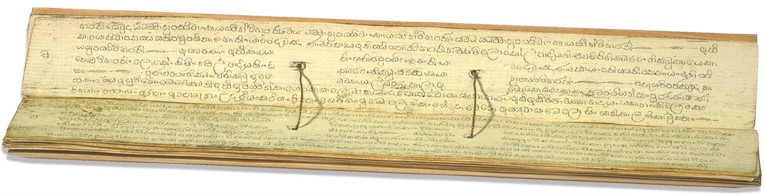
\includegraphics[width=0.7\linewidth]{./Diagrams/Palm}
\caption{These were the kinds of books created during the 4\textsuperscript{th} council and they are still created today.}
\label{fig:Palm}
\end{figure}

Moggaliputta Tissa sent out missionaries after the Third Council and this is how Buddhism was introduced to Sri Lanka at the Mahāvihāra.\footnote{\url{http://en.wikipedia.org/wiki/Anuradhapura_Maha_Viharaya}} For more than 200 years, the Mahāvihāra was the only Buddhist school in Sri Lanka. About 2000 years ago, the Sri Lankan King decided to introduce a new Buddhist school from India, the Abhayagiri\footnote{\url{http://en.wikipedia.org/wiki/Abhayagiri_vihara}} School. The Mahāvihāra now had competition and no longer had royal support. This was one of the factors contributing to the Fourth Council,\footnote{\url{http://en.wikipedia.org/wiki/Fourth_Buddhist_council}} when the Mahāvihāra monks went to a cave away from the royal capital to write their version of the \textit{Tipiṭaka} texts on palm leaves. Once the \textit{Tipiṭaka} had been committed to writing it was more difficult to change, so it is likely that the \textit{Tipiṭaka} that we have today was more or less finalized by the time of the Fourth Council.\footnote{The Fifth Council (\url{http://en.wikipedia.org/wiki/Fifth_Buddhist_council}) and the Sixth Council (\url{http://en.wikipedia.org/wiki/Sixth_Buddhist_council}) were held in Myanmar in 1871 and 1954. They involved a recitation and confirmation of the \textit{Tipiṭaka}.}

Reminds me of a joke: after 2000 years of copying the Buddhist texts, they realized that early on somebody had made a mistake and forgotten the “R”; the original word was “celebrate.”

\subsection*{Buddhaghosa’s Commentaries\footnote{The Visuddhimagga was written and the Commentaries were compiled about 1000 years after the Buddha’s \textit{parinibbāna} and in a cultural environment that was different from when the Buddha taught. This book is a modern scholar’s attempt to interpret the Buddha’s teachings in their original context: \url{http://www.ahandfulofleaves.org/documents/What the Buddha Thought_Gombrich_2009.pdf}}}

When the Chinese pilgrim monk Faxian\footnote{\url{http://en.wikipedia.org/wiki/Faxian}} visited Sri Lanka in 400 AD, he observed that the Abhayagiri School had 5000 monks, another school closely related to the Abhayagiri School\footnote{The Jetavana School (\url{http://en.wikipedia.org/wiki/Jetavanaramaya}).} had 2000 monks while the Mahāvihāra School had 3000 monks. In other words, 70 percent of the monks in Sri Lanka were not from the Mahāvihāra School. The monks from the Mahāvihāra School were feeling threatened.\footnote{Around 1200 AD the Mahāvihāra gained royal support and were able to eliminate the competing schools.} They were using Pāḷi while their competitors were using Sanskrit. They were seen as conservatives who had nothing new to offer while their competitors were introducing new Mahāyāna practices from India.\footnote{The competition also had a popular meditation manual called the Vimuttimagga, “The Path of Freedom”: (\url{http://en.wikipedia.org/wiki/Vimuttimagga}). Buddhaghosa’s Visuddhimagga was the Theravāda replacement for the Vimuttimagga. The Vimuttimagga and the Visuddhimagga have the same general structure of \textit{Sīla}, \textit{Samādhi} and \textit{Paññā}, but the Vimuttimagga is more practical while the Visuddhimagga is comprehensive and scholarly.} 

Based in the Mahāvihāra, Buddhaghosa\footnote{\url{http://en.wikipedia.org/wiki/Buddhaghosa}} wrote the Visuddhimagga.\footnote{\url{http://en.wikipedia.org/wiki/Visuddhimagga} (Path of Purification, see footnote 2).} Wikipedia describes the Visuddhimagga as a complete and coherent explanation of the \textit{Tipiṭaka} using the “Abhidhamma method.” Buddhaghosa also compiled Commentaries\footnote{The Visuddhimagga was written first and is referenced in many places in the Commentaries. The Visuddhimagga and the Commentaries provide background stories to the Suttas, word by word analysis of the Suttas, definitions and etymological information for important terms. The Visuddhimagga and the Commentaries are strongly influenced by the Abhidhamma.} for most of the texts in the \textit{Tipiṭaka}, based on Sinhalese materials accumulated in the library of the Mahāvihāra.\footnote{Buddhaghosa considered himself to be a compiler and translator of earlier material (not an author) and rarely offered his own views. Everything that he wrote would have been reviewed by the elders of the Mahāvihāra to confirm that it was aligned with the Theravāda doctrine.}

For the Mahāvihāra School, the Commentaries served three purposes. First, they reintroduced Pāḷi as an important language, not a dead language. Second, they presented the Mahāvihāra doctrine and reinforced the importance of the Abhidhamma. Third, they presented all the accumulated traditional accounts to capture the interest of the lay community. Actually, most of the stories about the life of the Buddha taught in Sunday Schools today are traditional accounts from the Commentaries.\footnote{The Suttas do not contain a lot of biographical material. For details of what is in the Suttas, see \url{http://store.pariyatti.org/Life-of-the-Buddha-The--PDF-eBook_p_1412.html}}

\subsection*{Abhidhammattha Sangaha}

The Abhidhammattha Sangaha is a very concise summary of the Abhidhamma and its Commentaries written in Sri Lanka about 1000 years ago. The Pāḷi text is only 46 pages long but it summarizes many thousands of pages of material. It was designed for young monks to memorize, without understanding. Once the monks were older, they would study the original Abhidhamma texts using what they had memorized in the Abhidhammattha Sangaha as a foundation. 

Today, most introductory Abhidhamma courses use the Abhidhammattha Sangaha as their textbook. Twenty years ago, Bhikkhu Bodhi\footnote{\url{http://en.wikipedia.org/wiki/Bhikkhu_Bodhi}} compiled a translation with explanatory notes and charts from Abhidhamma scholars called, “A Comprehensive Manual of Abhidhamma.”\footnote{PDF can be downloaded using the link in Footnote 2. Bhikkhu Bodhi's book is based on Nārada's “A Manual of Abhidhamma” (\url{http://www.buddhanet.net/pdf_file/abhidhamma.pdf}).} With the explanatory notes and charts added, the book is 400 pages long. If, after listening to my Practical Abhidhamma Course, you want to dive deeper into the technical details of the Abhidhamma, I highly recommend this book.\footnote{A three-volume transcript of lectures given by Sayādaw U Sīlānanda using Bhikkhu Bodhi’s book:\\ \url{http://www.abhidhamma.com/Abhid-Lectures-1.pdf}\linebreak \url{http://www.abhidhamma.com/Abhid-Lectures-2.pdf} \linebreak \url{http://www.abhidhamma.com/Abhid-Lectures-3.pdf}} Bhikkhu Bodhi’s book is quite technical and detailed. If you are looking for a book that is a bit lighter, I recommend “Abhidhamma in Daily Life” by Nina van Gorkom.\footnote{\url{http://archive.org/details/AbhidhammaInDailyLife}}

\subsection*{Abhidhamma today}

Let’s look at Abhidhamma today. The Abhidhamma is viewed very differently in the three major Theravāda countries: Myanmar,\footnote{\url{http://en.wikipedia.org/wiki/Buddhism_in_Burma}\linebreak\url{http://www.buddhanet.net/pdf_file/bud-myanmar.pdf}} Sri Lanka\footnote{\url{http://en.wikipedia.org/wiki/Buddhism_in_Sri_Lanka}\linebreak\url{http://www.buddhanet.net/pdf_file/bud-srilanka.pdf}} and Thailand.\footnote{\url{http://en.wikipedia.org/wiki/Buddhism_in_Thailand}\linebreak\url{http://www.buddhanet.net/pdf_file/bud-thailand.pdf}}

In Myanmar, Abhidhamma has been studied actively for 900 years.\footnote{“Study of the Abhidhamma amongst the Laity in Myanmar:” \url{http://atbu.org/node/10}} Two hundred fifty years ago, the government was holding exams on Abhidhamma for monks and laypeople.\footnote{The Abhidhamma increased in popularity about 100 years ago when Ledi Sayādaw started promoting \textit{vipassanā} and Abhidhamma for laypeople.} To give you an idea of how popular Abhidhamma is in Myanmar today, in 2005 almost 14,000 laypeople took the basic Abhidhamma exam at 124 government-run centres. Of all of the Theravāda countries, Abhidhamma is most widely studied in Myanmar. Novice monks start studying the Abhidhamma from the age of 13. The Burmese Sayādaws, particularly the meditation teachers, are extremely knowledgeable in Abhidhamma and frequently reference the Abhidhamma during their talks on meditation.

Today in Sri Lanka, the Abhidhamma is studied as an academic topic.\footnote{For example, “The Theravāda Abhidhamma” by Y. Karunadasa and “Abhidhammic Interpretations of Early Buddhist Teachings” by G. D. Sumanapala compare Theravāda Abhidhamma with Abhidharma from other schools.} The Abhidhamma is highly respected in Sri Lanka but rarely mentioned by monks in their Dhamma talks. The late chief monk at the Sri Lankan Vihāra where I teach, Dr. K Sri Dhammananda,\footnote{\url{http://en.wikipedia.org/wiki/K._Sri_Dhammananda}} gave Dhamma talks for 50 years, but I am not aware of him ever talking about Abhidhamma. However, in my early years of teaching,\footnote{I have been teaching Abhidhamma for 15 years at the Buddhist Mahā Vihāra in Kuala Lumpur, Malaysia: \url{http://buddhistmahavihara.org/}} whenever I had a difficult question about Abhidhamma, Chief always had an answer for me.

\pagebreak

In Thailand, the Abhidhamma is generally respected but often not studied in detail as it is in Myanmar.\footnote{The Thais do incorporate the Abhidhamma into a series of funeral chants called the “Abhidhamma \textit{Paṃsukūla}.” This includes 7 brief chants, each chant summarizing one of the books of the Abhidhamma \textit{Piṭaka}. These chants are intended to remind the mourners of the doctrines of \textit{anicca}, \textit{dukkha} and \textit{anattā}.} This is particularly true within the Thai Forest Tradition.\footnote{\url{http://en.wikipedia.org/wiki/Thai_Forest_Tradition}} Many western Theravāda monks are ordained in the Thai Forest Tradition and receive little training in the Abhidhamma. I consider this to be unfortunate, because western audiences are scientifically minded and, to quote a lay Burmese Abhidhamma teacher, “Abhidhamma is the Ultimate Science.”\footnote{The title of Dr. Mehm Tin Mon’s translation of the Abhidhammattha Sangaha with Commentary: \url{http://www.buddhanet.net/pdf_file/abhidhaultsci.pdf}} I believe that, if properly presented, Abhidhamma would be extremely popular in the West because it is so scientific, and can be applied both to daily life and to meditation practice.

\subsection*{Linkage to \textit{Satipaṭṭhāna} Sutta\footnote{For an analysis of the \textit{Satipaṭṭhāna} Sutta see \url{http://santifm.org/santipada/wp-content/uploads/2012/08/A_History_of_Mindfulness_Bhikkhu_Sujato.pdf} and \url{http://www.buddhismuskunde.uni-hamburg.de/pdf/5-personen/analayo/direct-path.pdf} }}
Now let’s relate this historical material to the \textit{Satipaṭṭhāna} Sutta.

There are two versions of the \textit{Satipaṭṭhāna} Sutta in the Sutta \textit{Piṭaka}; the version you have in the handout in front of you is from the \textit{Majjhima Nikāya}, and there is another version in the \textit{Dīgha Nikāya}.\footnote{DN 22: \url{http://www.accesstoinsight.org/tipitaka/dn/dn.22.0.than.html}} The two versions are virtually identical, except that the version in the \textit{Dīgha Nikāya} adds a long explanation of the Four Noble Truths. If the Commentaries are correct and all the Suttas were actually finalized at the First Council, we have to ask ourselves, “Which version did the Buddha actually teach on that day?”

When Xuanzang returned to China, he took back two versions of the \textit{Satipaṭṭhāna} Sutta from non-Theravāda Buddhist schools. The three versions, the Theravāda version and the two Chinese versions, are quite similar so it is clear they came from a common source that existed before the split of the Sangha.\footnote{For details, see “A Comparative Study of the Majjhima Nikāya,” Volume 1, pages 73--97.} One difference between the three versions is that the Chinese versions do not include the aggregates or the Four Noble Truths. If the version of the \textit{Satipaṭṭhāna} Sutta that existed before the split of the Sangha did include the aggregates and the Four Noble Truths, it is unlikely they would have been deleted by the other schools because these are core teachings. Therefore, I believe that the aggregates and Four Noble Truths were added to the Theravāda version of the \textit{Satipaṭṭhāna} Sutta sometime after the split of the Sangha. The aggregates and Four Noble Truths are core teachings of the Buddha, but I believe that their incorporation into the \textit{Satipaṭṭhāna} Sutta was a later addition.

I have picked one part of the \textit{Satipaṭṭhāna} Sutta to illustrate this point, but evidence of additions, editing and rearrangement, can be found in many other Suttas as well. In my opinion, the Suttas were not finalized at the First Council; the Suttas evolved over time. My conclusion is that the Theravāda Suttas that we have today contain the teachings of the Buddha, but they are \textbf{not} the literal, verbatim “word of the Buddha.” Personally, I am not disturbed by this because to me, it is the \textbf{teachings} that are important; the words merely point to the teachings.

\pagebreak

\begin{figure}[H]
\begin{tabular*}{\textwidth}{L{\dimexpr0.5\textwidth-2\tabcolsep} | L{\dimexpr0.5\textwidth-2\tabcolsep}}
\toprule
\tableheader{Structure of the Satipaṭṭhāna Sutta\newline from the Abhidhamma Piṭaka} & \tableheader{Structure of the Satipaṭṭhāna Sutta\newline from the Majjhima Nikāya} \\
\midrule
\textbf{The Contemplation of the Body} & \textbf{The Contemplation of the Body} \\
& Mindfulness of Breathing \\
& Postures of the Body \\
& Mindfulness with Clear Comprehension \\
Reflection on the Repulsiveness of the Body & Reflection on the Repulsiveness of the Body \\
& Reflection on the Material Elements \\
& Nine Cemetery Contemplations\\
& \\
\textbf{The Contemplation of Feeling} & \textbf{The Contemplation of Feeling} \\
Types of Feeling & Types of Feeling \\
& \\
\textbf{The Contemplation of Consciousness} & \textbf{The Contemplation of Consciousness} \\
Types of Consciousness & Types of Consciousness \\
& \\
\textbf{The Contemplation of Mental Objects} & \textbf{The Contemplation of Mental Objects} \\
Five Hindrances & Five Hindrances \\
& Five Aggregates of Clinging \\
& Six Internal and Six External Sense Bases \\
Seven Factors of Enlightenment & Seven Factors of Enlightenment \\
& Four Noble Truths\\

\bottomrule

\end{tabular*}
\caption{Comparing the Satipaṭṭhāna Sutta from the Abhidhamma Piṭaka (Vibhaṅga) and the Satipaṭṭhāna Sutta from the Majjhima Nikāya suggests that the Abhidhamma version may be earlier and that additions may have been made (from other Suttas) to the Majjhima Nikāya version.}
\label{fig:Satipatthana}
\end{figure}

We do not even have to look at other Buddhist schools to find inconsistency in the \textit{Satipaṭṭhāna} Sutta. One of the seven books of the Abhidhamma\footnote{“The Book of Analysis” (\textit{Vibhaṅga}), pages 251--270.} includes an essay that analyzes \textit{Satipaṭṭhāna} from both the Sutta perspective, and from an Abhidhamma perspective. The Abhidhamma text quotes the complete \textit{Satipaṭṭhāna} Sutta. This version of the Sutta found in the Abhidhamma does not include the aggregates or Four Noble Truths under the Contemplation of Mental Objects.

There is an even bigger inconsistency when looking at the Contemplation of the Body. The \textit{Satipaṭṭhāna} Sutta from the \textit{Majjhima Nikāya} includes \textbf{Mindfulness} of breathing, postures of the body, mindfulness with clear comprehension, reflection on the repulsiveness of the body, reflection on the material elements and nine cemetery contemplations. The \textit{Satipaṭṭhāna} Sutta from the Abhidhamma includes only reflection on the repulsiveness of the body. My conclusion is that from the time that this portion of the Abhidhamma was finalized, and the time that the \textit{Satipaṭṭhāna} Sutta from the \textit{Majjhima Nikāya} was finalized, sections were added to include \textbf{Mindfulness} of breathing, postures of the body, \textbf{Mindfulness} with clear comprehension, reflection on the material elements and nine cemetery contemplations. In other words, I believe that the Abhidhamma and the Suttas was evolving in parallel.

\subsection*{Summary of Key Points}

Here is a summary of key points from the Historical Development of the Abhidhamma:

\begin{itemize}

\item Buddhist teachings come from four periods: the Suttas and Vinaya, the Abhidhamma, the Commentaries and from modern teachers. The teachings of each period build on teachings of the previous periods. To provide context, it is useful to know the period from which a teaching comes.

\item According to the traditional account from the Commentaries, the Buddha first taught the Abhidhamma in one of the heavens and then passed a summary to Sāriputta, who compiled the Abhidhamma texts that we have today (except for one book which was authored about 250 years later).

\item According to scholars, about 100 years after the Buddha’s \textit{parinibbāna}, when the Sangha split, the main Buddhist doctrines were already fixed, though the Suttas were still subject to editing. At this time, the organization of Suttas into \textit{Nikāyas} was in progress and the Abhidhamma had not been formalized.

\begin{itemize}

\item In my opinion, the Abhidhamma is not the “word of the Buddha,” but I also believe that the Suttas are not the  literal, verbatim “word of the Buddha;” in my opinion, the Abhidhamma was evolving while the Suttas were being finalized and this can be seen by comparing the version of the \textit{Satipaṭṭhāna} Sutta found in the Abhidhamma with the version found in the \textit{Nikāyas}.

\end{itemize}

\item Factors that contributed to the development of the Abhidhamma may include:

\begin{itemize}

\item The need for a systematized structure covering all Suttas to resolve questions and to instruct novice monks.

\item A reaction to the trend among contemporary “atomist” philosophers to identify “irreducible components” or Ultimate Realities.

\item The need to organize the content of the Suttas in a way that emphasized the unique doctrines of the Theravāda school.

\end{itemize}

\item Buddhaghosa’s Visuddhimagga and the Commentaries make extensive use of the Abhidhamma; they were written in the fifth century.

\item The Abhidhammattha Sangaha is a summary of the Abhidhamma and Commentaries, intended for novice monks to memorize; it was written in the tenth century.

\item Today, the Abhidhamma is highly esteemed in Myanmar, often treated as an academic subject in Sri Lanka and often not studied in detail in Thailand.

\end{itemize}

Finally, in my opinion, the most important thing to remember about this talk is that there are four sources of teachings: Suttas, Abhidhamma, Commentaries and modern teachers. Each builds on the earlier sources. Knowing the source of a specific teaching helps to provide context.

\begin{center}
\textbf{\textit{This concludes the second talk.}} \\
\end{center}

\newpage

\subsection*{Questions \& Answers}

\question{Where does “The Questions of King Milinda” fit into this timeline?}

\begin{figure}[H]
\begin{quoting}
\topsep=0pt
\begin{flushleft}
\vspace{-1mm}
\textit{By what name shall I know you, Sir?}
\vspace{-1mm}
\end{flushleft}
\begin{flushright}
\vspace{-1mm}
\textit{My companions call me Nāgasena. But the name and the\linebreak person to whom the name refers do not really exist.}
\vspace{-1mm}
\end{flushright}
\begin{flushleft}
\vspace{-1mm}
\textit{If Nāgasena and the person do not exist, to whom do\linebreak people offer alms and who receives these offerings?\linebreak Since you receive them, you really exist.}
\vspace{-1mm}
\end{flushleft}
\begin{flushright}
\vspace{-1mm}
\textit{Your Majesty, did you come to this\linebreak monastery on foot or by chariot?}
\vspace{-1mm}
\end{flushright}
\begin{flushleft}
\vspace{-1mm}
\textit{I came by chariot.}
\vspace{-1mm}
\end{flushleft}
\begin{flushright}
\vspace{-1mm}
\textit{Well then, what is a chariot? Is the horse the chariot?\linebreak Is the wheel the chariot? Is the axle the chariot?\linebreak Is the carriage the chariot?}
\vspace{-1mm}
\end{flushright}
\begin{flushleft}
\vspace{-1mm}
\textit{I must answer “No” to all of your questions.}
\vspace{-1mm}
\end{flushleft}
\begin{flushright}
\vspace{-1mm}
\textit{Is there a thing called chariot beside the horse,\linebreak the wheel, the axle, the carriage, etc.?}
\vspace{-1mm}
\end{flushright}
\begin{flushleft}
\vspace{-1mm}
\textit{There is no chariot beside the horse, the wheels,\linebreak the axle and the carriage. Just a combination of\linebreak these things has been named a chariot.}
\vspace{-1mm}
\end{flushleft}
\begin{flushright}
\vspace{-1mm}
\textit{Very well, your Majesty, you should understand\linebreak Nāgasena as you understood the chariot.}
\vspace{-1mm}
\end{flushright}
\end{quoting}

\caption{King Milinda meets Nāgasena; the “components of the chariot” are the five aggregates (see also \url{http://www.accesstoinsight.org/tipitaka/sn/sn05/sn05.010.bodh.html}). }
\label{fig:Milinda}
\end{figure}

“The Questions of King Milinda” was written about 2100 years ago.\footnote{See \url{http://www.aimwell.org/milinda.html} and \url{http://en.wikipedia.org/wiki/Milinda_Panha}} It is included in the Burmese \textit{Tipiṭaka} but not in the Thai or Sri Lankan \textit{Tipiṭaka}.

It is written in the form of a dialogue between King Milinda and a Buddhist Monk, Nāgasena. King Milinda was an actual historical figure, a Greek king who ruled the kingdom of Bactria.\footnote{The Greek kingdom of Bactria (\url{http://en.wikipedia.org/wiki/Bactria}), in modern-day Afghanistan, was established by Alexander the Great. King Milinda (Greek name: Menander I, (\url{http://en.wikipedia.org/wiki/Menander_I}) ) extended the kingdom into North India and converted to Buddhism. Milinda and his successors were supporters of Buddhism. The first representations of the Buddha as a human date from this period and even today, paintings and statues of the Buddha show a Greek influence (\url{http://en.wikipedia.org/wiki/Greco-Buddhist_art}). Interestingly, the Suttas clearly state that the Buddha was bald, but even today all representations of the Buddha show him with a full head of hair! For the first 500 years, the Buddha was represented by an icon such as a stupa, footprint, bodhi tree, or wheel rather than as a human.} In a typical exchange, King Milinda would ask a philosophical question\footnote{The questions posed by King Milinda demonstrate a knowledge of the Suttas and show an influence of the Upaniṣads rather than an influence of Greek philosophy.} and Nāgasena would then give a reply using an analogy to explain his point clearly. 

\question{According to the traditional account, the Abhidhamma came before the Suttas and the Vinaya, so why isn't the Abhidhamma the first \textit{Piṭaka}?}

The \textit{Tipiṭaka} is not organized chronologically. For example, the first Sutta delivered by the Buddha, the Dhammacakkappavattana Sutta (SN 56.11: \url{http://www.accesstoinsight.org/tipitaka/sn/sn56/sn56.011.harv.html}) is located near the end of the third \textit{Nikāya}.

\question{Are you suggesting that we prioritise teachings based on the historical period in which they originate?}

Some modern teachers such as Mahāsi Sayādaw and Ajahn Chah add significant value to what had been taught previously in the Suttas, Abhidhamma and Commentaries. However, there are a few modern teachers who misrepresent the earlier teachings (either unintentionally due to ignorance or intentionally due to arrogance).

Not everything presented in Dhamma talks or in Dhamma books comes from the Suttas. Building up a habit of asking oneself, “what is the original source for this idea?” does not mean to be critical or analytical,\footnote{Trying to identify the specific Sutta or source text is being analytical and can be a distraction.} it simply means to be aware of the context of a teaching. Remember that one of the qualities of the Dhamma is \textit{ehipassiko}, which means “inviting inspection.” 

\question{You mentioned that different schools have different versions of Abhidhamma. How do we know that we are studying the right one?}

In my opinion, we should not think in terms of “right” or “wrong,” but rather, how useful the Abhidhamma is in deepening our understanding of the Suttas and in supporting our practice. If history had worked out a bit differently, we might be studying one of the other versions of Abhidhamma today, but as it is, we have the Theravāda version as a living tradition with many resources available. In my opinion, we should focus on the practical aspects rather than on a scholarly perspective.

\question{Mindfulness Based Stress Reduction (MBSR) is becoming popular. Can the Abhidhamma be applied to MBSR?}

Mindfulness Based Stress Reduction\footnote{\url{http://en.wikipedia.org/wiki/Mindfulness-based_stress_reduction}} was developed 25 years ago by an American mental health professional.\footnote{Dr. Jon Kabat-Zinn: \url{http://en.wikipedia.org/wiki/Jon_Kabat-Zinn}} The MBSR program\footnote{Described in \url{http://www.amazon.com/Full-Catastrophe-Living-Wisdom-Illness/dp/0739358588}} is a pure mindfulness exercise, similar in some ways to basic \textit{vipassanā} meditation practice, but without spiritual content (as the name suggests, MBSR is for stress reduction). Even though MBSR does not lead to spiritual development, according to WebMD, depression affects almost one in six people at some point in their lives,\footnote{\url{http://www.webmd.com/depression/ss/slideshow-depression-myths}} so the secular practice of MBSR can help our society. 

In my opinion, for the mental health industry to take MBSR to the next level, they will need a framework and standardized, specialized terminology to structure their discussions and analyze the mind in more detail. I believe that many aspects of the Abhidhamma can be re-purposed to a secular context to accelerate this progress.

\pagebreak

\question{What is the relationship between the Visuddhimagga and the Commentaries?}

Buddhaghosa wrote the Visuddhimagga and was the compiler/translator of the Commentaries.

According to legend,\footnote{Chapter XXXVII of the Cūḷavamsa, written 800 years after Buddhaghosa died.} Buddhaghosa was born near Bodh Gaya\footnote{\url{http://en.wikipedia.org/wiki/Bodh_Gaya}} to a Brahmin\footnote{\url{http://en.wikipedia.org/wiki/Brahmin}} family. In the Indian caste system, Brahmins were priests who memorized and recited the Vedas.\footnote{\url{http://en.wikipedia.org/wiki/Vedas}} As a young man, Buddhaghosa established himself as a famous debater. A Buddhist monk, Revata, decided to convert Buddhaghosa to Buddhism. One day while Buddhaghosa was reciting the Vedas, Revata called out, “Who is this man, braying like a donkey?” Buddhaghosa replied, “So, you think that you understand the language of a donkey?” and the debate started! Revata proved that he understood the Vedas and pointed out areas where they were wrong. Defeated, Buddhaghosa asked, “So what is your doctrine?” Revata then quoted from the Abhidhamma and Buddhaghosa could not respond. Buddhaghosa was deeply impressed by the Abhidhamma. He was converted to Buddhism and that is when he got the name Buddhaghosa. \textit{Ghosa} is Pāḷi for “voice” so the name Buddhaghosa literally means “voice of the Buddha”.

Revata told Buddhaghosa to go to the Mahāvihāra in Sri Lanka to compile the commentaries that had been collected in Sinhalese and translate them into Pāḷi. Buddhaghosa went to the Mahāvihāra and said to the temple elders, “Please open up your library to me.” The elders replied, “To show that you are worthy, write an essay on the topic of virtue, concentration and understanding.” So Buddhaghosa composed the Visuddhimagga, an 800-page treatise detailing the Theravāda doctrine that draws heavily on the Abhidhamma.

After Buddhaghosa wrote the Visuddhimagga, the gods made the book disappear, so he had to write it down again. Again the gods made this version disappear, so Buddhaghosa wrote the book a third time. Then the gods allowed the previous two versions to be visible and the elders were amazed that all three versions were absolutely identical. A later legend says that Buddhaghosa wrote the Visuddhimagga out three times in one night. 

The elders were impressed by the Visuddhimagga and allowed Buddhaghosa access to the library. Buddhaghosa compiled commentaries on most of the Vinaya, Suttas and Abhidhamma. For the commentaries, Buddhaghosa saw himself as a compiler/translator of much older materials, some of which may have originated at the time of the Buddha 1000 years earlier.

Whereas the Visuddhimagga focuses on explaining Theravāda doctrine, the Commentaries focus on explaining the Vinaya, Suttas and Abhidhamma. The Commentaries include a lot of stories, such as the background leading up to a Sutta being delivered. They also discuss grammatical points and word derivations to make sure that the Vinaya, Suttas and Abhidhamma are clearly understood. When it comes to doctrinal points, the Commentaries often reference the Visuddhimagga; this shows that the Visuddhimagga was written before the Commentaries. 

Though Buddhaghosa prepared Commentaries for most of the \textit{Tipiṭaka}, the Commentaries for some portions of the \textit{Tipiṭaka} were complied later by other authors. In addition, sub-commentaries were written for many of the Commentaries to provide even more detailed explanations.

\question{What are the main differences between the Abhidhammattha Sangaha and the original seven Abhidhamma texts?}

The Abhidhammattha Sangaha is a concise summary written almost 1500 years after the original seven Abhidhamma texts. The main topics of the Abhidhammattha Sangaha are:

\begin{itemize}

\item Mind Moments: Both the Abhidhammattha Sangaha and the original text (\textit{Dhammasaṅgaṇī}) include 89 Mind Moments, though the sequence of presentation is slightly different.

\item Mental Factors: The Abhidhammattha Sangaha has a fixed list of 52 Mental Factors. The original text (\textit{Dhammasaṅgaṇī}) has open-ended lists that include many overlapping terms but do not mention Mental Factors such as \textbf{Attention}, \textbf{Determination}, \textbf{Motivation}, \textbf{Compassion}, \textbf{Sympathetic joy} and the three abstinences.

\item \textit{Rūpa}: The Abhidhammattha Sangaha has a fixed list of 28 \textit{rūpa} and discusses groups of \textit{rūpa} (\textit{kalāpa}). The original text (\textit{Dhammasaṅgaṇī}) has a fixed list of 27 \textit{rūpa} (not including \textbf{Heart-base}) and does not discuss groups of \textit{rūpa}.

\item Realms of Existence: Both the Abhidhammattha Sangaha and the original texts have the same list of realms of existence. The Abhidhammattha Sangaha gives a detailed analysis of Mind Moments leading to rebirth in specific realms. The original text (\textit{Vibhaṅga}) just mentions the lifespan in each realm.

\item Processes: The Abhidhammattha Sangaha has a detailed description of sense-door processes, mind-door processes, jhāna processes and rebirth processes. The original text (\textit{Paṭṭhāna}) hints at processes and the Commentaries have a very general description of only the sense-door process.

\item Conditions: The Abhidhammattha Sangaha has a very concise summary of the 24 conditions and introduces sub-categories under some conditions (for example, natural decisive support is introduced as a sub-category under decisive support condition). The original text (\textit{Paṭṭhāna}) has a very detailed description of the 24 conditions.

\item Meditation Subjects: The Abhidhammattha Sangaha describes the meditation subjects for both \textit{samatha} and \textit{vipassanā}. The original texts do not touch on this subject; it is discussed in some detail in the Visuddhimagga.

\end{itemize}

%\section{Consciousness (\textit{Citta})}

Welcome to the third lesson of this Practical Abhidhamma Course. This lesson describes consciousness, the first of the four Ultimate Realities: \textit{citta}, \textit{cetasika}, \textit{rūpa} and \textit{Nibbāna}.\footnote{See Chapter 1 of “A Comprehensive Manual of Abhidhamma” (see Footnote 2 for link).}

\subsection*{Definition of Consciousness}

Let’s start with a definition of consciousness. I downloaded the Wikipedia entry on “consciousness” and it filled 18 pages.\footnote{\url{http://en.wikipedia.org/wiki/Consciousness}} Obviously, “consciousness” is not a simple thing to define. I do, however, like the first sentence from the Wikipedia entry: “Consciousness is the quality or state of awareness, or, of being aware of an external object or something within oneself.”

There are two important things in this definition. First, consciousness and awareness are synonyms. Second, consciousness always takes an object; either an external object or an internal object.\footnote{Object condition (\textit{ārammaṇa-paccaya}); see Chapter 3 of “The Conditionality of Life” (see Footnote 2 for link).} A \textbf{Sound} is an example of an external object. When the mind is aware of itself, it takes an internal object such as \textbf{Attachment}.

The Commentary defines consciousness as having three roles. First, consciousness is that which is aware of an object; there is no Self that is aware, it is consciousness that is aware. Second, consciousness allows the associated Mental Factors to be aware of an object. And third, consciousness is an activity, a process of being aware of an object.

\subsection*{Definition of Mind Moment}

\begin{figure} [H]

\vspace{-1mm}

\begin{quote}
Life, personhood, pleasure and pain; this is all that's bound together in a single mental event, a moment that quickly takes place.

Even the spirits who endure for 84,000 aeons, even these, do not live the same for any two moments of mind.

What ceases for one who is dead, or for one who's still standing here, are all just the same aggregates; gone, never to connect again.

The states which are vanishing now, and those which will vanish some day, have characteristics no different than those that have vanished before.

\end{quote}

\caption{The concept of a Mind Moment is captured in this extract from a beautiful poem found in the Suttas (Nm 2.4: \url{http://www.accesstoinsight.org/tipitaka/kn/nm/nm.2.04.olen.html}).}

\end{figure}

Consciousness never arises alone; it always arises as part of a Mind Moment. A Mind Moment is consciousness together with its associated Mental Factors. The Abhidhamma describes Mind Moments and Mental Factors in detail and these are the topics of this lesson and the next lesson.

\pagebreak

Within a Mind Moment, consciousness and each of its associated Mental Factors work as an inseparable team, each with their own characteristic. Consciousness has the characteristic of knowing the object. Each Mental Factor has its own individual characteristic such as grasping the object or not floating away from the object.\footnote{“Grasping the object” is the characteristic of \textbf{Attachment}, “not floating away from the object” is the characteristic of \textbf{Mindfulness}.}

As mentioned in the first lesson, according to the Commentaries, what is conventionally called the mind is modelled as a sequence of Mind Moments, like a “stream of consciousness.” Each Mind Moment arises based on conditions, performs its function and then falls away again.

\subsection*{Brief descriptions of each group of Mind Moments}

\begin{figure} [H]

\setlength{\tabcolsep}{0pt}
\renewcommand{\arraystretch}{1.0}
\noindent\begin{tabular}{C{.04\textwidth}C{0.16\textwidth}C{0.16\textwidth}C{0.16\textwidth}C{0.16\textwidth}C{0.16\textwidth}C{0.16\textwidth}}
\toprule
& \tablesubheader{{\small Unwholesome}} & \tablesubheader{{\small Rootless}} & \tablesubheader{{\small Wholesome}} & \tablesubheader{{\small Fine Material Sphere}} & \tablesubheader{{\small Immaterial Sphere}} & \tablesubheader{{\small Supra-\newline mundane}} \\
\midrule
\tablevsubheader{{\small \hspace{-2mm}Create New Kamma}} & Danger\newline Zone\newline \textbf{1}--\textbf{12} & & Faultless\newline Zone\newline \textbf{31}--\textbf{38} & {\small Fine Material Sphere Wholesome} \textbf{55}--\textbf{59} & {\small Immaterial Sphere Wholesome} \textbf{70}--\textbf{73} & {\small Supramundane Path}\newline \textbf{82}--\textbf{85} \\
\midrule
\tablevsubheader{{\small \hspace{-2mm}Result of Kamma}} & & Sensing\newline Zone\newline \textbf{13}--\textbf{27} & {\small Sense Sphere Resultant}\newline \textbf{39}--\textbf{46} & {\small Fine Material Sphere Resultant} \textbf{60}--\textbf{64} & {\small Immaterial Sphere Resultant} \textbf{74}--\textbf{77} & {\small Supramundane Fruit}\newline \textbf{86}--\textbf{89} \\
\midrule
\tablevsubheader{{\small \hspace{-2mm}Unrelated to Kamma}} & & Sensing\newline Zone\newline \textbf{28}--\textbf{29} & {\small Sense Sphere Functional}\newline \textbf{47}--\textbf{54} & {\small Fine Material Sphere Functional} \textbf{65}--\textbf{69} & {\small Immaterial Sphere Functional} \textbf{78}--\textbf{81} & \\
\bottomrule
\end{tabular}
\caption{A simplified overview of Appendix 2. Numbers in bold represent Mind Moments. The Danger Zone, the Faultless Zone and the Sensing Zone are the most important areas.}
\label{Handout3}
\end{figure}

Appendix 2 lists Mind Moments numbered from \textbf{1}--\textbf{89}. We will refer back to it many times during other lessons as well. Consider it to be a ``map of the mind." With this map, you can explore without getting lost! 

Figure \ref{Handout3} summarizes the content of Appendix 2. In this map of the mind, Mind Moments are grouped together in rows and columns. I will first give a brief description of each group and then do an in-depth analysis of some of the groups.

\pagebreak

The first group are Mind Moments \textbf{1}--\textbf{12}. These create unwholesome\footnote{The Pāḷi term for unwholesome is \textit{akusala}, the opposite of \textit{kusala}; the prefix “\textit{a}” signifies the “active opposite of,” not merely “absence of.” The Commentary defines \textit{kusala} as “healthy,” “faultless” and “producing happy results.” Therefore, \textit{akusala} means “unhealthy,” “faulty,” and “producing unhappy results.”} kamma. I call this the “Danger Zone.”\footnote{Other Abhidhamma texts do not use the term, “Danger Zone.”} The Danger Zone is engulfed in a dense fog of \textbf{Delusion}, so it is impossible for the mind to see where it is, where it is going, or that this is the “Danger Zone.” In part of the Danger Zone sticky quicksand traps the mind, these are the \textbf{Attachment}-rooted Mind Moments. Another part of the Danger Zone is burning hot and painful for the mind; these are the \textbf{Aversion}-rooted Mind Moments.

The second group are Mind Moments \textbf{13}--\textbf{29}. These Mind Moments are involved in the sensing and processing of sense data and ideas. I call this the “Sensing Zone.”\footnote{Other Abhidhamma texts do not use the term, “Sensing Zone.”}

The third group are Mind Moments \textbf{31}--\textbf{38}. These create wholesome kamma. I call this the “Faultless Zone.”\footnote{The Abhidhammattha Sangaha classifies Mind Moments \textbf{31}--\textbf{54} as being “beautiful” (\textit{sobhana}). Abhidhamma texts do not use the term, “Faultless Zone,” but “faultless” is used as a translation of “\textit{kusala}.”} In this zone there is no \textbf{Attachment}, only \textbf{Non-attachment}. There is no \textbf{Aversion}, only \textbf{Non-aversion}. In some parts of the Faultless Zone, details of everything can be clearly seen, and these parts are the Mind Moments associated with \textbf{Understanding}.

In a Sutta called “Two Sorts of Thinking,” the Buddha stressed the importance of knowing if the mind is in the Danger Zone or the Faultless Zone.\footnote{MN 19: \url{http://www.accesstoinsight.org/tipitaka/mn/mn.019.than.html}} If the mind is in the Danger Zone, the Buddha advises us to reflect on the disadvantages of such thinking. If it is in the Faultless Zone, just be passively aware. In this Sutta, the Buddha also said that whatever you keep thinking about will become the inclination of your awareness. In other words, unwholesome thinking accumulates into an unwholesome perspective and unwholesome habits. Similarly, wholesome thinking accumulates into a wholesome perspective and wholesome habits.

\begin{figure}[h]
\centering
\input{./Diagrams/Life_Cont.pdf_tex}
\caption{Many Life-continuum Mind Moments arise between each Sensing/Thinking Process and during dreamless sleep.}
\label{fig:Life_Cont}
\end{figure}

The fourth group (Sense Sphere Resultant) are Mind Moments \textbf{39}--\textbf{46}. The main function of these Mind Moments is Life-continuum.\footnote{The Pāḷi term for Life-continuum is \textit{bhavaṅga}; literally factor (\textit{aṅga}) of existence (\textit{bhava}). The only reference to \textit{bhavaṅga} in the Abhidhamma \textit{Piṭaka} is in “Conditional Relations” (\textit{Paṭṭhāna}), Volume I page 159 and elsewhere, where it is described as preceding five-sense-door adverting (Mind Moment \textbf{28}).} These Mind Moments arise during dreamless sleep, and between all the sensing and thinking that goes on while we are awake; they arise when the mind is not sensing, not thinking and not in a jhāna\footnote{\url{http://en.wikipedia.org/wiki/Dhyana_in_Buddhism}} meditative state.

The fifth group (Sense Sphere Functional) are Mind Moments \textbf{47}--\textbf{54}. These arise only in the mind of an Arahat.\footnote{\url{http://en.wikipedia.org/wiki/Arhat}} Mind Moments \textbf{47}--\textbf{54} correspond to Mind Moments \textbf{31}--\textbf{38}, except that Mind Moments \textbf{47}--\textbf{54} do not create new kamma as Arahats do not create new kamma.

The sixth group (Fine Material Sphere Wholesome) are Mind Moments \textbf{55}--\textbf{59}. These arise during the five Fine Material jhānas and create wholesome kamma.

The seventh group (Fine Material Sphere Resultant) are Mind Moments \textbf{60}--\textbf{64}. These do not arise in humans; they are the Life-continuum Mind Moments for beings in higher Realms of Existence.

The eighth group (Fine Material Sphere Functional) are Mind Moments \textbf{65}--\textbf{69}. These arise only in the mind of an Arahat, when an Arahat experiences a Fine Material jhāna.

The ninth group (Immaterial Sphere Wholesome) are Mind Moments \textbf{70}--\textbf{73}. These arise during the four Immaterial jhānas and create wholesome kamma.

The tenth group (Immaterial Sphere Resultant) are Mind Moments \textbf{74}--\textbf{77}. These do not arise in humans; they are the Life-continuum Mind Moments for beings in much higher Realms of Existence.

The eleventh group (Immaterial Sphere Functional) are Mind Moments \textbf{78}--\textbf{81}. These arise only when an Arahat experiences an Immaterial jhāna.

The twelfth group (Supramundane Path) are Mind Moments \textbf{82}--\textbf{85}. These path Mind Moments arise at the moment of transition to each degree of sainthood. 

The thirteenth group (Supramundane Fruit) are Mind Moments \textbf{86}--\textbf{89}. These fruit Mind Moments allow a saint to enjoy the bliss of \textit{Nibbāna}. 

The Pāḷi name for the twelfth and thirteenth groups is translated as Supramundane, literally “transcending the world.”\footnote{\textit{Lokuttara}, combines world (\textit{loka}) and transcending (\textit{uttara}).} These Mind Moments take \textit{Nibbāna} as their object and are reserved for saints and for the Buddha.

\subsection*{Using this ``map of the mind" (Appendix 2 and Figure \ref{Handout3})}

Before we go into the details of Mind Moments, let’s take a step back and consider the question, “How can I use this map of the mind?”

To develop spiritually we need to look at the mind. If the mind is agitated, we need first to steady, settle, unify and compose the mind; perhaps by focusing on a neutral object such as the breath. When we look inwards with a calm mind, the most obvious Mind Moments will be in the Danger Zone (Mind Moments \textbf{1}--\textbf{12}) or in the Faultless Zone (Mind Moments \textbf{31}--\textbf{38}).

If unwholesome Mind Moments are found when looking at the mind, don’t be frustrated. Frustration is another unwholesome Mind Moment. If unwholesome Mind Moments are found, be mindful of their characteristics; “Ah, this is the grasping of \textbf{Attachment}.” or “Ah, the mind is experiencing \textbf{Aversion}.” Mindfulness converts the unwholesome Mind Moment into a wholesome Mind Moment with \textbf{Understanding}. As mentioned earlier, when facing unwholesome mind moments, the Buddha recommended an active approach of reflecting on the disadvantages of such thinking.

If wholesome Mind Moments are found when looking at the mind, don’t be attached to them; craving wholesome Mind Moments brings craving, an unwholesome Mind Moment. If wholesome Mind Moments are found, just be mindful of their characteristics; “Ah, the mind is calm, not floating away.” As mentioned earlier, when facing wholesome mind moments, the Buddha recommended a passive approach of just being aware.

Here is a \textbf{\textit{RADICAL}} approach to ``moment to moment mindfulness" based on a modern author.\footnote{Sayālay Susīlā: \url{http://www.sayalaysusila.net/files/Moment-to-Moment-Practice.pdf}} It is a traditional approach, but the word \textbf{\textit{RADICAL}} is used as an acronym. The \textbf{\textit{RADICAL}} approach is \textbf{\textit{R}}ecognize, \textbf{\textit{A}}ccept, \textbf{\textit{D}}epersonalize, \textbf{\textit{I}}nvestigate, \textbf{\textit{C}}ontemplate \textbf{\textit{A}}nicca or \textbf{\textit{C}}ontemplate \textbf{\textit{A}}nattā, and \textbf{\textit{L}}et go.

\pagebreak

\textbf{\textit{R}}ecognize means identifying the current Mind Moment.

\textbf{\textit{A}}ccept means accepting what is experienced just as it is; resisting the unpleasant is \textbf{Aversion}, and clinging to the pleasant is \textbf{Attachment}. 

\textbf{\textit{D}}epersonalize means being a stable observer, separate and unbiased; what is experienced is not “happening to me,” it is not “myself,” it is not “mine,” it simply is something to be observed. 

\textbf{\textit{I}}nvestigate is the point at which \textbf{Understanding} starts to play an important role. Look closely; what is experienced has characteristics that can be understood. 

\textbf{\textit{CA}} means Contemplate \textit{Anicca} or Contemplate \textit{Anattā}. Notice that what is experienced is impermanent or is a natural process, not Self. 

Finally, \textbf{\textit{L}}et go because there is always a new experience waiting.

%To repeat, the \textbf{\textit{RADICAL}} approach is \textbf{\textit{R}}ecognize, \textbf{\textit{A}}ccept, \textbf{\textit{D}}epersonalize, \textbf{\textit{I}}nvestigate, \textbf{\textit{C}}ontemplate \textbf{\textit{A}}nicca or \textbf{\textit{C}}ontemplate \textbf{\textit{A}}nattā, and \textbf{\textit{L}}et go. 

We are so obsessed with the urgent that we neglect the important. Why not make a habit of regularly dedicating a few moments to mindfulness using the \textbf{\textit{RADICAL}} approach? This will slowly train the mind. Just as the body benefits from regular exercise, the mind can also benefit from regular 
use of the \textbf{\textit{RADICAL}} approach.

\subsection*{Mind Moments 1--12 (Danger Zone)}

\begin{figure}[H]

\setlength{\tabcolsep}{0pt}
\renewcommand{\arraystretch}{1.1}
\begin{center}
\begin{tabular}{P{.05\textwidth}L{.15\textwidth}L{.2\textwidth}C{.05\textwidth}}
\toprule
\multicolumn{4}{c}{\tablesubheader{\textbf{Attachment}-rooted}}\\
\textbf{1} & Unprompted & Wrong view & \smiley \\
\textbf{2} & Prompted & Wrong view & \smiley \\
\textbf{3} & Unprompted & No wrong view & \smiley \\
\textbf{4} & Prompted & No wrong view & \smiley \\
\textbf{5} & Unprompted & Wrong view & \neutral \\
\textbf{6} & Prompted & Wrong view & \neutral \\
\textbf{7} & Unprompted & No wrong view & \neutral \\
\textbf{8} & Prompted & No wrong view & \neutral \\
\multicolumn{4}{c}{\tablesubheader{\textbf{Aversion}-rooted}} \\
\textbf{9} & Unprompted & Ill will & \frowney \\
\textbf{10} & Prompted & Ill will & \frowney \\
\multicolumn{4}{c}{\tablesubheader{\textbf{Delusion}-rooted}} \\
\textbf{11} & \multicolumn{2}{l}{Associated with doubt} & \neutral \\
\textbf{12} & \multicolumn{2}{l}{Associated with restlessness} & \neutral \\
\bottomrule
\end{tabular}
\end{center}
\begin{center}
\smiley\hspace{2mm} Pleasant \textbf{Feeling}\hspace{5mm}\neutral\hspace{2mm} Indifferent \textbf{Feeling}\hspace{5mm}\frowney\hspace{2mm}Unpleasant \textbf{Feeling}
\end{center}
\caption{The Danger Zone: Mind Moments \textbf{1}--\textbf{12} create unwholesome kamma.}
\label{fig:Danger}
\end{figure}

Let’s look at the Danger Zone, Mind Moments \textbf{1}--\textbf{12}, in more detail. This group is subdivided into \textbf{Attachment}-rooted, \textbf{Aversion}-rooted and \textbf{Delusion}-rooted. These three unwholesome roots of \textbf{Attachment}, \textbf{Aversion} and \textbf{Delusion} are frequently  mentioned in the Suttas.\footnote{Iti 3.50: \url{http://www.accesstoinsight.org/tipitaka/kn/iti/iti.3.050-099.than.html\#iti-050}} Just as roots provide a foundation, support, strength and nourishment to a tree, a Mind Moment gets a foundation, support, strength and nourishment from its roots.\footnote{This is root condition (\textit{hetu-paccaya}); see Chapter 2 of “The Conditionality of Life” (see Footnote 2 for link).}

\pagebreak

In the Kālāma Sutta, the Buddha was asked how to evaluate teachings.\footnote{AN 3.65: \url{http://www.accesstoinsight.org/tipitaka/an/an03/an03.065.than.html}} The Buddha first advised the Kālāmas not to judge teachings based on tradition, conjecture or the charisma of the teacher.\footnote{At the time of the Buddha, there were three approaches to knowledge: oral tradition (from the ancient \textit{Vedas}: \url{http://en.wikipedia.org/wiki/Vedas}), logical reasoning (the basis of the recently-developed Upaniṣads: \url{http://en.wikipedia.org/wiki/Upanishads}, teachings of religious philosophy), and direct intuition of a teacher. In MN 100 (\url{http://metta.lk/tipitaka/2Sutta-Pitaka/2Majjhima-Nikaya/Majjhima2/100-sangarava-e1.html}), the Buddha put himself in the third category. See \url{http://www.ahandfulofleaves.org/documents/Early Buddhist Theory of Knowledge_Jayatilleke.pdf}} The Buddha then asked if \textbf{Attachment}, \textbf{Aversion} and \textbf{Delusion} were beneficial or unbeneficial, and if \textbf{Non-attachment}, \textbf{Non-aversion} and \textbf{Understanding} were beneficial or unbeneficial. The Kālāmas said that \textbf{Attachment}, \textbf{Aversion} and \textbf{Delusion} were unbeneficial and \textbf{Non-attachment}, \textbf{Non-aversion} and \textbf{Understanding} were beneficial. The Buddha then told the Kālāmas that teachings were good if they led to a decrease in \textbf{Attachment}, \textbf{Aversion} and \textbf{Delusion} and led to an increase in \textbf{Non-attachment}, \textbf{Non-aversion} and \textbf{Understanding}. This simple guideline can be applied when considering the motivation behind our own actions.

\subsubsection*{\textbf{Attachment}-rooted}

Mind Moments \textbf{1}--\textbf{8} are \textbf{Attachment}-rooted. Earlier, I referred to these Mind Moments as the sticky quicksand that traps the mind in the foggy Danger Zone. Sticky quicksand refers to the root of \textbf{Attachment} which is the primary characteristic of these Mind Moments. These eight Mind Moments also have a root of \textbf{Delusion}; this is the thick fog. They are in the Danger Zone because they create unwholesome kamma.

Reminds me of a joke: the young novice monk asks his teacher, “Master, is it allowable for a monk to use email?” The teacher replies, “Sure, as long as there are no attachments.”\footnote{From my experience, \textbf{Attachment} to email is a significant distraction during a meditation retreat. Yogis may want to turn off data (to avoid email and instant messages) and tell people to send an SMS in case of emergency.}

\textbf{Attachment} has many grades, ranging from simply enjoying a coffee to intense passion. A subtle form of \textbf{Attachment} is \textbf{Attachment} to sense objects; the desire to see things, to hear things, etc. There is a story in the Suttas warning about sense-desires.\footnote{SN 47.7: \url{http://www.accesstoinsight.org/tipitaka/sn/sn47/sn47.007.than.html}. Suttas warning of the dangers of sense-desires are directed at monks, who have already overcome most of the attachments faced by laypeople.} A hunter puts tar on a branch. The foolish monkey is curious and touches the tar with one hand. The hand gets stuck, so the monkey uses his other hand, his two feet and finally his mouth to try to get free. The monkey is then trapped in five ways, corresponding to the five senses-desires. 

I prefer the modern version of this story in which the hunter attaches a hollowed-out coconut to a tree.\footnote{See \url{http://en.wiktionary.org/wiki/monkey_trap}} Food is put inside the coconut to attract the monkey. The monkey grabs the food but with a clenched fist full of food, it is unable to extract its hand so it is trapped. I prefer this version because to free itself, the monkey just has to overcome its instinctive \textbf{Attachment} to the food and open its hand. Of course, overcoming instinctive \textbf{Attachment} is easier said than done for the monkey, and for the monkey’s distant cousins, we humans!

As you can see from Figure \ref{fig:Danger}, the eight Mind Moments in the \textbf{Attachment}-rooted group include every combination of unprompted or prompted, associated or not associated with \textbf{Wrong view}, and pleasant or indifferent \textbf{Feeling}.

\pagebreak

The first differentiating factor is unprompted or prompted. An unprompted Mind Moment arises spontaneously; if I do something without anybody trying to convince me, then the Mind Moment behind the action is unprompted. A prompted Mind Moment has to be instigated or induced by another person or by myself; if I need convincing to do something, then the Mind Moment is prompted. Prompting is not triggered by the object, prompting is related to influence by another person or oneself.

The second differentiating factor, either “associated with \textbf{Wrong view}” or “not associated with \textbf{Wrong view},” is extremely important, so let’s discuss \textbf{Wrong view} in a bit more detail. \textbf{Wrong view} is an opinion, a bias or a judgement that can impact one’s outlook, perspective, paradigm or belief.

Almost 500 years ago, Copernicus wrote that observations and calculations showed that the earth orbited the sun; that the earth is not the centre of the universe.\footnote{\url{http://en.wikipedia.org/wiki/Nicolaus_Copernicus}} Initially, the idea was ignored. Sixty years after Copernicus’ death, only 15 astronomers in all of Europe agreed. The idea was ignored because it challenged the prevailing “common sense” and church doctrine.

In the first lesson, I shared a scientific experiment showing that a “Self who decides” is an illusion created after a decision has already been made; there is no Self at the centre of the universe. I suspect that after an initial discomfort with the results of the experiment, your mind ignored results of the experiment because the ego-centric view of the universe is “common sense.” “Ignored” is a verb; the related noun is “ignorance” or mental blindness. Refusing to see things as they truly are is clinging to ignorance or \textbf{Attachment} to \textbf{Wrong view}.

But we don’t need a fancy experiment to show the illusion of a controlling Self. Consider the last time that confusion arose in the mind. Was there a conscious decision at that time? Was there a Self who said, “I think that I will choose to be confused now?” Of course not! Confusion arose naturally. After confusion arose, Self-identification took place, “I am confused.”

\begin{figure}[H]
\centering
\input{./Diagrams/Latent.pdf_tex}
\caption{\textit{\small The process by which latent defilements lead to \textbf{Wrong view} and how this reinforces the latent defilements.}}
\label{fig:Latent}
\end{figure}

A distorted view arises because of the latent defilements.\footnote{Latent defilements (\textit{anusaya}) are sensual desire, \textbf{Aversion}, \textbf{Wrong view}, \textbf{Doubt}, \textbf{Conceit}, desire for existence and \textbf{Delusion}; see AN 7.11: \url{http://www.accesstoinsight.org/tipitaka/an/an07/an07.011.than.html}} I will illustrate this process using two analogies; a man afraid of snakes and a woman craving spiritual progress.

\pagebreak

Imagine a man with a fear of snakes.\footnote{This famous analogy is used by Candrakirti in his Commentary on Aryadeva’s “Catuḥśataka.”} Most of the time, this fear has no impact on his life. The fear is latent, not arisen, and he may not even be aware of this fear. The man is walking down a dimly-lit path at night and there is a coil of rope ahead. His latent fear of snakes causes him to misperceive the coil as a snake. This distorted perception, combined with his latent fear of snakes, causes him to think about snakes. This distorted thinking, combined with his latent fear of snakes, convinces the man that there is a snake ahead. This distorted view causes the fear of snakes to arise. It is no longer a latent fear. This actual fear reinforces his latent tendency to be afraid of snakes.\footnote{Distortion of \textbf{Perception} is \textit{saññāvipallāsa}, distortion of thought is \textit{cittavipallāsa} and distortion of view is \textit{diṭṭhivipallāsa}. Others have translated \textit{vipallāsa} as “inversions” or “perversions;” \textit{Vipallāsa} is literally \textit{vi} + \textit{pari} + \textit{āsa} = “turned upside down.”} In other words, actual fear comes from latent fear plus distorted view, distorted view comes from latent fear plus distorted thought, distorted thought comes from latent fear plus distorted perception, and distorted perception comes from latent fear.

Imagine a woman who is attached to the idea of spiritual progress. This is a latent \textbf{Attachment}, waiting for a trigger to arise. While sitting on her cushion one day, some mundane experience arises in the woman’s mind. Her \textbf{Attachment} to spiritual progress causes her to misperceive the mundane experience as an insight. Driven by this distorted perception, and supported by her \textbf{Attachment} to the idea of spiritual progress, she thinks she has experienced an insight. This distorted thought, supported by her \textbf{Attachment} to the idea of spiritual progress convinces her that she has experienced an insight. This distorted view causes \textbf{Attachment} to arise. It is no longer a latent \textbf{Attachment}. This actual \textbf{Attachment} reinforces her latent tendency to be attached to the idea of spiritual progress.

\begin{figure}[H]

\centering

\includegraphics[width=0.8\linewidth]{./Diagrams/Cats}
\caption{\textbf{Delusion} distorts reality. \textbf{Wrong view} sees something that does not really exist (for example, the ego creates a huge “Self”).}
\label{fig:Cats}
\end{figure}

\textbf{Delusion} is mental blindness, while \textbf{Wrong view} involves conviction that something that is wrong is correct. As you can see from the examples of the snake and the woman's insight, \textbf{Delusion} triggers distorted perception, \textbf{Delusion} and distorted perception trigger distorted thought, then \textbf{Delusion} and distorted thought trigger \textbf{Attachment} to \textbf{Wrong view}. When \textbf{Attachment} to \textbf{Wrong view} arises, the underlying \textbf{Delusion} is reinforced.

\pagebreak

\begin{figure}[H]
\centering

\includegraphics[width=0.9\linewidth]{./Diagrams/Perception}
\caption{Latent tendencies influence how an image is perceived; do you perceive the first image as a vase or as two faces? Psychologists use the Rorschach inkblot test (\url{http://en.wikipedia.org/wiki/Rorschach_test}), such as the second image, to gain insights into a person’s latent tendencies.}
\label{fig:Perception}
\end{figure}

The Buddha listed four types of \textbf{Wrong view} that are harmful to spiritual progress.\footnote{AN 4.49: \url{http://www.accesstoinsight.org/tipitaka/an/an04/an04.049.than.html}} First, taking what is impermanent as permanent is \textbf{Wrong view}. Second, taking what is unsatisfactory as pleasant is \textbf{Wrong view}. Third, taking what is impure to be pure is \textbf{Wrong view}. Fourth, taking what is non-self as Self is \textbf{Wrong view}. The Buddha frequently highlighted the danger of taking what is non-self as Self.\footnote{According to Visuddhimagga XXII.68 (see Footnote 2 for link) the Sotāpanna uproots all four types of \textit{diṭṭhivipallāsa} (no speech or action because of \textit{vipallāsa}). \textit{Saññāvipallāsa} and \textit{cittavipallāsa} related to \textit{anicca} and related to \textit{anattā} are also uprooted by the Sotāpanna. \textit{Saññāvipallāsa} and \textit{cittavipallāsa} related to \textit{asubha} are uprooted by the Anāgāmī. \textit{Saññāvipallāsa} and \textit{cittavipallāsa} related to \textit{dukkha} are uprooted by the Arahat.} He explained how the ego of the untrained mind twists and distorts whatever is perceived, to place a Self at the centre by imagining a relationship with what is experienced.\footnote{MN 1: \url{http://www.accesstoinsight.org/tipitaka/mn/mn.001.than.html}} The experience of pain becomes “my pain,” “I am in pain” or “it is painful to me.” All of this happens in the blink of an eye. The Buddha’s teachings, our own experience, and scientific experiments all tell us that “Self is an illusion.” In spite of all this evidence, we stubbornly cling to the \textbf{Wrong view} of Self.

The third differentiating factor is pleasant \textbf{Feeling} or indifferent \textbf{Feeling}. Dictionary.com\footnote{\url{http://dictionary.reference.com/browse/feeling}} has 14 definitions for “feeling.” In Buddhism, \textbf{Feeling} has one definition; the most basic experience of pleasant, unpleasant or indifferent.\footnote{The Abhidhamma identifies five types of \textbf{Feeling}: mental pleasant, mental unpleasant, mental indifferent, physical pleasant (pleasure) and physical unpleasant (pain).} When we see the word \textbf{Feeling} in the Suttas or Abhidhamma, it is important that we put aside all other meanings associated with the English word “feeling,” and think of \textbf{Feeling} as describing only a pleasant, unpleasant or indifferent experience. Later, we will discuss the contemplation of \textbf{Feeling} in the \textit{Satipaṭṭhāna} Sutta.

The \textbf{Attachment}-rooted Mind Moments are subdivided according to prompting, \textbf{Wrong view} and \textbf{Feeling}; this subdivision may have been done to reflect the relative weightiness of the associated kamma. A Mind Moment that is unprompted or spontaneous may create weightier kamma than a prompted Mind Moment that depends on somebody else, or depends on self-reflection. A Mind Moment associated with \textbf{Wrong view} may create weightier kamma than a Mind Moment not associated with \textbf{Wrong view}.\footnote{For example, Milindapañha III,7,8 explains that a person who picks up a hot object unknowingly will suffer greater burns than a person who picks up a hot object knowingly.} A Mind Moment accompanied by pleasant \textbf{Feeling} may create weightier kamma than a Mind Moment accompanied by indifferent \textbf{Feeling}. Spontaneity, association with \textbf{Wrong view} and pleasant \textbf{Feeling} may all contribute to increase the \textbf{Volition} of a Mind Moment, and weightiness of kamma depends on the level of \textbf{Volition}.

\pagebreak

Consider a boy spontaneously stealing an apple, with joy, convinced that there is nothing wrong with stealing. The boy’s Mind Moment is unprompted, associated with \textbf{Wrong view} and accompanied by pleasant \textbf{Feeling}. It is Mind Moment \textbf{1}.

Imagine that, knowing lying is wrong, I reluctantly compliment someone to make them happy. My Mind Moment is prompted, not associated with \textbf{Wrong view}, and accompanied by indifferent \textbf{Feeling}. It is Mind Moment \textbf{8}.

I am not saying that stealing the apple resulted in weightier kamma than giving a false compliment. Rather, I am saying that stealing the apple spontaneously probably created weightier kamma than if the boy had to be convinced by his friend to steal it. The weightiness of kamma depends on the strength of the underlying \textbf{Volition}, so it is difficult to compare different actions.

This weightiness of kamma has a parallel in our legal system. Is a judge not more likely to give a stiffer punishment if a defendant is happy they committed a crime or think that they did nothing wrong? Is a judge not more likely to be more lenient if a defendant was forced to commit the crime or committed the crime reluctantly?

\subsubsection*{\textbf{Aversion}-rooted}

Now let’s look at Mind Moments rooted in \textbf{Aversion}. Mind Moment \textbf{9} is unprompted and Mind Moment \textbf{10} is prompted. Earlier, I referred to these Mind Moments as burning hot and painful because they are accompanied by unpleasant \textbf{Feeling}. While the eight \textbf{Attachment}-rooted Mind Moments are attracted to the object, these two Mind Moments do not like their object or are not satisfied with their object.

Just as \textbf{Attachment} has many grades, from simply enjoying coffee to intense passion, \textbf{Aversion} also has many grades. \textbf{Aversion} could be as subtle as not accepting the object as it is, or as intense as blinding hatred. When there is fear, there is \textbf{Aversion} toward a future situation. When there is \textbf{Remorse} or regret, there is \textbf{Aversion} toward a past situation. When there is boredom, there is \textbf{Aversion} toward the current situation. When there is \textbf{Envy}, there is \textbf{Aversion} because I do not like that somebody has something that I do not. Hatred, anger, fear, \textbf{Remorse}, boredom and \textbf{Envy} are all accompanied by unpleasant \textbf{Feeling}.

Which Mind Moment arises at the moment a hunter kills for sport? Before killing, the hunter was looking for the animal and these Mind Moments would have been rooted in craving or \textbf{Attachment}. At the moment of killing, the hunter does not want the animal to continue living, so the Mind Moment is rooted in \textbf{Aversion}; not necessarily \textbf{Aversion} to the animal, but rather \textbf{Aversion} to the situation that the animal is alive. Since the killing is premeditated, the Mind Moment is prompted. This is Mind Moment \textbf{10}. After the killing, the hunter may be proud of his accomplishment and again, the Mind Moments would be rooted in \textbf{Attachment}.

The Buddha was once insulted by a Brahmin. The Buddha replied, “If you offer food to a guest and the guest refuses it, does the food not then belong to you? Similarly, I do not accept the insults that you have offered, so they are all yours.”\footnote{SN 7.2: \url{http://www.accesstoinsight.org/tipitaka/sn/sn07/sn07.002.than.html}}

We all know that hatred is never conquered by hatred, only by loving-kindness.\footnote{Dhammapada verse 5: \url{http://www.tipitaka.net/tipitaka/dhp/verseload.php?verse=005}}

\pagebreak

Here is an analogy about dealing with anger. Imagine we want to stop the steam coming from a pot of boiling water on the stove. The short-term quick fix, the one that we are immediately drawn to, is to put a lid on the pot to keep the steam from escaping while pressure builds up inside the pot. The person who sees things as they truly are understands that it is the nature of steam to arise when there is a source of heat. This person stops the steam by turning off the stove. Imagine that we are angry and getting ready to blow off steam. Short-term quick fix techniques such as “firm resolution,” “considering the Buddha’s example” and “considering the harmful effects of anger” deal with the symptoms. It is impossible to overcome anger using a strategy based on \textbf{Aversion} to the current situation. Only beautiful Mental Factors such as \textbf{Mindfulness}, \textit{mettā} and \textbf{Understanding} deal with the root cause and turn off anger at the source.

We may blame external things such as a person, a situation, etc. when \textbf{Aversion} arises, but actually the cause of \textbf{Aversion} is internal. Eleanor Roosevelt said, “No one can make you feel inferior without your consent.”\footnote{\url{http://en.wikipedia.org/wiki/Eleanor_Roosevelt}\linebreak {\url{http://www.goodreads.com/author/quotes/44566.Eleanor_Roosevelt}}} This applies to all forms of \textbf{Aversion}, not just feeling inferior.

Over the years, I have been asked many times, “How do I get rid of anger?” but nobody has ever asked “How do I stop enjoying my coffee?” To quote Rudyard Kipling, we need to “meet with triumph and disaster and treat those two impostors just the same.”\footnote{\url{http://en.wikipedia.org/wiki/Rudyard_Kipling} \newline \url{http://www.poetryfoundation.org/poem/175772}} The Buddha identified eight worldly conditions as gain and loss, status and disgrace, praise and blame, pleasure and pain.\footnote{AN 8.6: \url{http://www.accesstoinsight.org/tipitaka/an/an08/an08.006.than.html}} The saint sees these eight worldly conditions as they truly are; impermanent. But when facing these eight worldly conditions, you and I get caught up in \textbf{Attachment} and \textbf{Aversion}.

\subsubsection*{\textbf{Delusion}-rooted}

All 12 of the Mind Moments in the Danger Zone include the root of \textbf{Delusion}. This is why I mentioned earlier that the entire Danger Zone was engulfed in a dense fog causing mental blindness. 

Reminds me of a joke: if ignorance is bliss, why aren’t more people happy?

\textbf{Attachment}-rooted Mind Moments have mental blindness working in the background, covering up the nature of the object. If the object is seen as impermanent, how can there be \textbf{Attachment}? \textbf{Aversion}-rooted Mind Moments also have mental blindness working in the background, covering up the nature of the object. If the object is seen as naturally arising because of conditions, how can there be \textbf{Aversion}? \textbf{Attachment} and \textbf{Aversion} cannot arise without \textbf{Delusion} doing its job in the background. \textbf{Delusion} is like a magician who can fool you. However, once you know how the magician performs his tricks, he can no longer deceive and captivate you; you are no longer fooled.

\textbf{Delusion} is also like the director of a film. You never see the director on the screen, but the director influences everything from the background. The director controls the script, actors, lighting, camera angle and the music of the film. Everything is coordinated by the director to manipulate the audience’s emotions; \textbf{Attachment} and \textbf{Aversion}. On the other hand, if you were on the set while they were making the movie, it would be obvious what was really happening.

\begin{figure}[H]
\centering

\includegraphics[width=1.0\linewidth]{./Diagrams/Actors}
\caption{The Buddha criticized actors for causing \textbf{Attachment}, \textbf{Aversion} and \textbf{Delusion} in other people. Many salespeople and politicians also cause \textbf{Attachment}, \textbf{Aversion} and \textbf{Delusion} in other people.}
\label{fig:Actors}
\end{figure}

The head of an acting troupe once asked the Buddha about the rebirth destination for an actor.\footnote{SN 42.2: \url{http://www.accesstoinsight.org/tipitaka/sn/sn42/sn42.002.than.html}} The Buddha replied that an actor could be reborn in hell or as an animal because they cause \textbf{Attachment}, \textbf{Aversion} and \textbf{Delusion} in other people.\footnote{In this Sutta, it is clear that the Buddha was referring to actors whose focus was entertainment; actors whose intention is to educate the audience regarding the human condition may not be included in this category.} 

Mind Moments \textbf{1}--\textbf{8} have both \textbf{Delusion} and \textbf{Attachment}. Mind Moments \textbf{9} and \textbf{10} have both \textbf{Delusion} and \textbf{Aversion}. Mind Moments \textbf{11} and \textbf{12} have \textbf{Delusion}, but no \textbf{Attachment} and no \textbf{Aversion}.

Mind Moment \textbf{11} is associated with \textbf{Doubt}. \textbf{Doubt} is not the same as not being sure about a person’s name. \textbf{Doubt} refers to the uncertainty in the benefit of generosity, uncertainty about the benefit of morality or uncertainty about the benefit of spiritual development. At the end of the previous lesson, I said that the Theravāda Suttas we have today contain the teachings of the Buddha, but they are \textbf{not} the literal, verbatim “word of the Buddha.” This may qualify under the general English language usage of the word “doubt,” but does not imply Mind Moment \textbf{11}.

\textbf{Doubt} cannot be reduced just by thinking; direct experience is the way to reduce \textbf{Doubt}. Here is a metaphor to show how \textbf{Doubt} is uprooted by the Sotāpanna’s experience of \textit{Nibbāna}. Imagine that you are on the near side of a stream and want to get to the far side.\footnote{The near side of the stream is Self-view; the Sotāpanna has eradicated Self-view. See SN 35.197: \url{http://www.accesstoinsight.org/tipitaka/sn/sn35/sn35.197.than.html}} You start by convincing yourself saying, “I can jump over this stream.” This is blind faith; there is still a lot of \textbf{Doubt} in the mind. You study books on stream jumping, you listen to talks on how to jump across streams, you read about previous stream-jumpers and now when you say, “I can jump over this stream,” there is less \textbf{Doubt}. On your side of the stream you practise jumping and become incredibly skilled, an Olympic-level jumper. Now when you say, “I can jump over this stream,” there is very little \textbf{Doubt}, but \textbf{Doubt} remains because you have not yet jumped over this stream. You jump over it and are now on the far side. Having jumped over the stream, there are no more conditions for \textbf{Doubt} to arise. There is not even the most subtle \textbf{Doubt} remaining. \textbf{Doubt} has been truly uprooted. Before this point, \textbf{Doubt} was increasingly reduced, but now and forever in the future, it has been uprooted.

Figure \ref{fig:Danger} indicates that Mind Moment \textbf{12} is associated with \textbf{Restlessness}. Actually, \textbf{Restlessness} arises in all of the unwholesome Mind Moments, but in Mind Moments \textbf{1}--\textbf{11}, \textbf{Restlessness} is in the background whereas in Mind Moment \textbf{12}, \textbf{Restlessness} is dominant.

\textbf{Restlessness} is the opposite of steadiness or calmness; it is confusion, unsteadiness, agitation, mental distraction or mental excitement. A restless mind is not interested in the object and treats the object superficially. 

Reminds me of a joke: If I had a dollar for every  time I was distracted, I wish I had some ice cream!

\textbf{Restlessness} arises very frequently, but most people are unaware of it. When a person first tries to meditate, they are often surprised at the \textbf{Restlessness} in the mind. It seems that the mind never wants to penetrate the object; that the mind is wild and untamed. To help meditators deal with \textbf{Restlessness}, the Buddha delivered a Sutta titled “The removal of distracting thoughts.”\footnote{MN 20: \url{http://www.accesstoinsight.org/tipitaka/mn/mn.020.soma.html}} The good news is that the \textbf{Volition} associated with Mind Moment \textbf{12} is very weak, so the unwholesome kamma created by a restless mind is not weighty.

\subsection*{Mind Moments 31--38 (Faultless Zone)}

\begin{figure}[H]

\setlength{\tabcolsep}{0pt}
\renewcommand{\arraystretch}{1.1}
\begin{center}
\begin{tabular}{P{.05\textwidth}L{.15\textwidth}L{.2\textwidth}C{.05\textwidth}}
\toprule
\multicolumn{4}{c}{\tablesubheader{Sense Sphere Wholesome}}\\
\textbf{31} & Unprompted & Understanding & \smiley \\
\textbf{32} & Prompted & Understanding & \smiley \\
\textbf{33} & Unprompted & No understanding & \smiley \\
\textbf{34} & Prompted & No understanding & \smiley \\
\textbf{35} & Unprompted & Understanding & \neutral \\
\textbf{36} & Prompted & Understanding & \neutral \\
\textbf{37} & Unprompted & No understanding & \neutral \\
\textbf{38} & Prompted & No understanding & \neutral \\
\bottomrule
\end{tabular}
\end{center}
\begin{center}
\smiley\hspace{2mm} Pleasant \textbf{Feeling}\hspace{5mm}\neutral\hspace{2mm} Indifferent \textbf{Feeling}
\end{center}
\caption{Mind Moments \textbf{31}--\textbf{38}: Faultless Zone.}
\label{fig:Faultless}
\end{figure}

Let’s now jump to Mind Moments that create wholesome kamma, Mind Moments \textbf{31}--\textbf{38}. Earlier, I called this the Faultless Zone. This group's subdivisions are “prompted and unprompted,” “with and without \textbf{Understanding}” and “pleasant and indifferent \textbf{Feeling}.” We have already discussed prompted and unprompted, and pleasant and indifferent \textbf{Feeling}; let’s now discuss \textbf{Understanding}.

In Pāḷi, the word for \textbf{Understanding} is \textit{Paññā}. The Abhidhamma considers \textit{Paññā} to be the foundation of wisdom, investigation, insight, right view and \textit{vipassanā}.\footnote{One Mental Factor listed in the Abhidhamma is often equivalent to multiple terms from the Suttas.} Mind Moments \textbf{31}--\textbf{38} will create wholesome kamma, and those Mind Moments associated with \textbf{Understanding} (Mind Moments \textbf{31}, \textbf{32}, \textbf{35} and \textbf{36}) will contribute to spiritual development.\footnote{Faultless Mind Moments without \textit{Paññā} may also contribute to spiritual development, depending on how one defines “spiritual development.” Mind Moments without \textit{Paññā} can establish a habit supporting the arising of future Mind Moments with \textit{Paññā}.}

\pagebreak

Just to be clear, \textbf{Understanding} or wisdom does not imply intelligence. There is a story in the Commentary of a monk who was unable to memorize a single verse after trying for four months, yet was able to become an Arahat.\footnote{\url{http://www.tipitaka.net/tipitaka/dhp/verseload.php?verse=025}}

Morality and thoughts of generosity always create wholesome kamma, and when associated with \textbf{Understanding}, this can also directly contribute to spiritual development. All forms of mental cultivation directly contribute to spiritual development. This includes meditation, studying the Dhamma, teaching the Dhamma and straightening of views.

So how do we apply \textbf{Understanding} in our daily life?\footnote{Taken from Visuddhimagga I.13 (see Footnote 2 for link).} Bad speech and bad action come from bad thoughts. Bad thoughts arise from latent tendencies. Working backwards, we start by addressing bad speech and bad actions through precepts, morality or virtue; in Pāḷi, this is called \textit{Sīla}. Bad thoughts are addressed through having a composed or concentrated mind; in Pāḷi, this is called \textit{Samādhi}. Latent tendencies are addressed through \textbf{Understanding} or \textit{Paññā}.

\begin{figure}[H]
\centering
\input{./Diagrams/Sila.pdf_tex}
\caption{Latent tendencies give rise to thoughts which are manifested as actions and speech. Sīla is the restraint of actions and speech, Samādhi calms the mind and Paññā exposes the latent tendencies.}
\label{fig:Sila}
\end{figure}

\textit{Sīla}, \textit{Samādhi} and \textit{Paññā} are progressive steps. Start with \textit{Sīla}, and that will support \textit{Samādhi} which is a condition for \textit{Paññā}. \textit{Paññā} deepens the quality of \textit{Sīla} leading to deeper \textit{Samādhi} and clearer \textit{Paññā}, and the cycle continues. The Noble Eightfold Path can also be analyzed in terms of \textit{Sīla}, \textit{Samādhi} and \textit{Paññā}. \textit{Sīla} is Right Speech, Right Action and Right Livelihood. \textit{Samādhi} is Right Effort, Right \textbf{Mindfulness} and Right Concentration. \textit{Paññā} is Right View and Right Thought.

The Commentary gives an analogy to explain the difference between perceiving, thinking and \textbf{Understanding} to emphasize that \textbf{Understanding} is not superficial. A baby, a child and a money-changer all see a coin. The baby perceives a shiny, round object. The child thinks, “This is money” and thinks about what money can buy, how money can be used. The money-changer understands the qualities of the coin and can detect a counterfeit coin. The baby perceives, the child thinks and the money-changer understands.

The Buddha talked about the blind men who each touch different parts of an elephant and then argue over “what is an elephant.”\footnote{Ud 6.4: \url{http://www.accesstoinsight.org/tipitaka/kn/ud/ud.6.04.than.html}} The blind men’s different perceptions led to incomplete thinking and arguments. \textbf{Understanding} would be viewing the big picture like the sighted person who can see the entire elephant. 

Reminds me of a joke: a group of blind elephants each touched different parts of a human with their foot and they all agreed that a human was flat.

Earlier, I mentioned how \textbf{Wrong view} comes from distorted perception and distorted thinking. The analogies of the snake, the coin and the elephant all remind us that we all are subject to distorted and incomplete perceptions, distorted and incomplete thinking. Assumptions can lead to \textbf{Wrong view} but investigation can lead to \textbf{Understanding}.

\pagebreak

\begin{figure} [H]
\begin{center}

\includegraphics[width=0.4\linewidth]{./Diagrams/Dana}
\end{center}
\caption{A mother and her child offer dāna to a monk.}
\label{fig:Dana}
\end{figure}

Let’s consider another example and identify its associated Mind Moment. A mother sees a monk on alms round through the window. Immediately, she collects some food and takes her young child outside. They both offer food to the monk. At the time of offering, the Mind Moment of the mother and the Mind Moment of the young child are both wholesome; the Mind Moments are in the Faultless Zone. The Mind Moment of the mother is unprompted, spontaneous, while the Mind Moment of the child is prompted and depended on the inducement of the mother. The Mind Moment of the mother is with \textbf{Understanding}; she sees this as part of her spiritual development, and the child’s Mind Moment is without \textbf{Understanding}; the child is too young to comprehend. The Mind Moment of the mother is accompanied by pleasant \textbf{Feeling} while the child’s Mind Moment may be accompanied by indifferent \textbf{Feeling}. Mother and child perform exactly the same action, but the mother’s kamma will be much weightier because her \textbf{Volition} was much stronger. The mother’s Mind Moment will be \textbf{31} and the child’s will be \textbf{38}. The mother’s Mind Moment \textbf{31} will directly contribute to her spiritual development. The child’s Mind Moment \textbf{38} may indirectly contribute to his spiritual development by establishing a habit of generosity; as the child gets older, generosity may arise with \textbf{Understanding} and directly contribute to his spiritual development.

\pagebreak

\subsection*{Mind Moments 13--29 (Sensing Zone)}

\begin{figure}[H]

\setlength{\tabcolsep}{0pt}
\renewcommand{\arraystretch}{1.1}
\begin{center}
\begin{tabular}{P{.05\textwidth}L{.3\textwidth}C{.05\textwidth}}
\toprule
 \multicolumn{3}{c}{\tablesubheader{Unwholesome Resultant}} \\
 \textbf{13} & Eye-consciousness & \neutral \\
 \textbf{14} & Ear-consciousness & \neutral \\
 \textbf{15} & Nose-consciousness & \neutral \\
 \textbf{16} & Tongue-consciousness & \neutral \\
 \textbf{17} & Body-consciousness & \frowney \\
 \textbf{18} & Receiving consciousness & \neutral \\
 \textbf{19} & Investigating consciousness & \neutral \\
 \multicolumn{3}{c}{\tablesubheader{Wholesome Resultant}} \\
 \textbf{20} & Eye-consciousness & \neutral \\
 \textbf{21} & Ear-consciousness & \neutral \\
 \textbf{22} & Nose-consciousness & \neutral \\
 \textbf{23} & Tongue-consciousness & \neutral \\
 \textbf{24} & Body-consciousness & \smiley \\
 \textbf{25} & Receiving consciousness & \neutral \\
 \textbf{26} & Investigating consciousness & \smiley \\
 \textbf{27} & Investigating consciousness & \neutral \\
\midrule
 \multicolumn{3}{c}{\tablesubheader{Functional}} \\
 \textbf{28} & Five-sense-door adverting & \neutral \\
 \textbf{29} & Determining consciousness & \neutral \\
\bottomrule
\end{tabular}
\end{center}
\begin{center}
\smiley\hspace{2mm} Pleasant \textbf{Feeling}\hspace{5mm}\neutral\hspace{2mm} Indifferent \textbf{Feeling}\hspace{5mm}\frowney\hspace{2mm}Painful \textbf{Feeling}
\end{center}
\caption{Mind Moments \textbf{13}--\textbf{29}: Sensing Zone. Note that Mind Moment \textbf{17} is with painful (physical) feeling and Mind Moment \textbf{24} is with pleasurable (physical) feeling.}
\label{fig:Sensing}
\end{figure}

We have covered the Danger Zone, Mind Moments \textbf{1}--\textbf{12}, and the Faultless Zone, Mind Moments \textbf{31}--\textbf{38}. Now let’s look at the Sensing Zone, Mind Moments \textbf{13}--\textbf{29}. These are involved in the sensing and processing of sense data and ideas. In a later lesson, I will go into the details of each of these Mind Moments, but at this point I will give only a brief overview of a few of them.

Mind Moments \textbf{13}--\textbf{17} and Mind Moments \textbf{20}--\textbf{24} are the sense-consciousness Mind Moments corresponding to the five physical senses. The Mind Moment that captures an image at the back of the retina can be either Mind Moment \textbf{13} or Mind Moment \textbf{20}; both are eye-consciousness Mind Moments. The only difference between them is that Mind Moment \textbf{13} is the result of unwholesome kamma, while Mind Moment \textbf{20} is the result of wholesome kamma.

Once the sense-consciousness Mind Moment has performed its function, the sense data is processed. Mind Moments \textbf{18} and \textbf{19} will process sense data that arose because of unwholesome kamma. Mind Moments \textbf{25} and either Mind Moment \textbf{26} or Mind Moment \textbf{27} will process sense data that arose because of wholesome kamma.

\pagebreak
\subsubsection*{Decision box}

\begin{figure}[H]
\centering
\input{./Diagrams/Room.pdf_tex}
\caption{Decision directs the flow of the mind from the input/trigger to one of the outputs.}
\label{fig:Room}
\end{figure}

Once sense data has been captured and processed, a decision needs to be made as to how to proceed. That decision is the function of Mind Moment \textbf{29} (Determining consciousness). If the object is an idea, then Mind Moments \textbf{13}--\textbf{28} are bypassed, and the mind jumps directly to Mind Moment \textbf{29} to make a decision. You will notice that Mind Moment \textbf{29} is unrelated to kamma. The mind does not make decisions because of kamma.

Let me give you an analogy to explain the interaction between the Danger Zone, the Faultless Zone and the Sensing Zone. Figure \ref{fig:Room} shows a “Decision box.” There is one entrance to the box from below and this is how a stimulus such as a \textbf{Visible-form}, \textbf{Sound}, idea, etc. enters the mind. There are three exits from the box leading to the Danger Zone and one exit from the box leading to the Faultless Zone.\footnote{Appendix 2 also shows a ``Decision box" connecting the sensing zone to the Danger/Faultless Zone.}

The exits are the mind’s reaction to the stimulus; the result of the decision made by Mind Moment \textbf{29}. The three exits to the left are based on \textbf{Attachment}, \textbf{Aversion} and \textbf{Delusion}, and lead to the Danger Zone. The exit to the right leads to the Faultless Zone.

In the previous lesson, I mentioned that the mind makes decisions naturally. I referred to experiments that show how the mind decides first, and then later the idea of a Self who decides is created. I mentioned that a concept of a Self is added by the mind as a justification or rationalization of the decision making process. Actually, it is the decisions made by Mind Moment \textbf{29} that determines how much time is spent in the Faultless Zone and how much time is spent in the Danger Zone.

So how does Mind Moment \textbf{29} decide? The answer is very simple: accumulations, not kamma. Wholesome accumulations naturally cause Mind Moment \textbf{29} to open the door to the Faultless Zone. Unwholesome accumulations naturally cause Mind Moment \textbf{29} to open one of the doors to the Danger Zone. So how can accumulations be changed or reinforced? The answer is very simple: training.

Simple is not the same as easy. The five precepts, the rules of training, are simple to understand, but keeping the precepts is sometimes difficult. I try to recite the five precepts at least once a day. When I recite them, I reflect deeply upon them. Repetitive actions done with strong \textbf{Volition} train the mind and reinforce accumulations.

Before moving on to the jhānas (Mind Moments \textbf{55}--\textbf{81}), I should briefly mention Mind Moment \textbf{30}. Mind Moment \textbf{30} is not involved with Sensing. This Mind Moment arises only in an Arahat or a Buddha and causes a smile. 

\pagebreak

\subsection*{Mind Moments 55--81}

\begin{figure}[H]
\setlength{\tabcolsep}{0pt}
\renewcommand{\arraystretch}{1.1}

\begin{center}
\noindent\begin{tabular}{P{.05\textwidth}L{0.15\textwidth}C{.05\textwidth}C{0.0295\textwidth}P{.05\textwidth}L{0.265\textwidth}C{.05\textwidth}}
\toprule
\multicolumn{3}{C{0.287\textwidth}}{\tablesubheader{Fine Material Sphere Wholesome}} & & \multicolumn{3}{c}{\tablesubheader{Immaterial Sphere Wholesome}}\\
\textbf{55} & First Jhāna & \smiley & & \textbf{70} & Infinity of space & \neutral \\
\textbf{56} & Second Jhāna & \smiley & & \textbf{71} & Infinity of consciousness & \neutral \\
\textbf{57} & Third Jhāna & \smiley & & \textbf{72} & Nothingness & \neutral \\
\textbf{58} & Fourth Jhāna & \smiley & & \textbf{73} & Neither perception nor & \neutral \\
\textbf{59} & Fifth Jhāna & \neutral & & & non-perception & \\
\midrule
\multicolumn{3}{C{0.287\textwidth}}{\tablesubheader{Fine Material Sphere Resultant}} & & \multicolumn{3}{c}{\tablesubheader{Immaterial Sphere Resultant}} \\
\textbf{60} & First Jhāna & \smiley & & \textbf{74} & Infinity of space & \neutral \\
\textbf{61} & Second Jhāna & \smiley & & \textbf{75} & Infinity of consciousness & \neutral \\
\textbf{62} & Third Jhāna & \smiley & & \textbf{76} & Nothingness & \neutral \\
\textbf{63} & Fourth Jhāna & \smiley & & \textbf{77} & Neither perception nor & \neutral \\
\textbf{64} & Fifth Jhāna & \neutral & & & non-perception & \\
\midrule
\multicolumn{3}{C{0.287\textwidth}}{\tablesubheader{Fine Material Sphere Functional}} & & \multicolumn{3}{c}{\tablesubheader{Immaterial Sphere Functional}} \\
\textbf{65} & First Jhāna & \smiley & & \textbf{78} & Infinity of space & \neutral \\
\textbf{66} & Second Jhāna & \smiley & & \textbf{79} & Infinity of consciousness & \neutral \\
\textbf{67} & Third Jhāna & \smiley & & \textbf{80} & Nothingness & \neutral \\
\textbf{68} & Fourth Jhāna & \smiley & & \textbf{81} & Neither perception nor & \neutral \\
\textbf{69} & Fifth Jhāna & \neutral & & & non-perception \\
\bottomrule
\end{tabular}
\end{center}

\begin{center}
\smiley\hspace{2mm} Pleasant \textbf{Feeling}\hspace{5mm}\neutral\hspace{2mm} Indifferent \textbf{Feeling}
\end{center}

\caption{Mind Moments \textbf{55}--\textbf{81}: Fine Material Sphere and Immaterial Sphere}
\label{fig:55to81}
\end{figure}

Let’s move to Mind Moments \textbf{55}--\textbf{69}, which relate to the jhānas. As the focus of these lessons is applying Abhidhamma to daily life, I will not spend a lot of time discussing jhāna practice. Jhāna practice pre-dates the Buddha; the Buddha talked about practising the jhānas before he was enlightened.\footnote{MN 26: \url{http://www.accesstoinsight.org/tipitaka/mn/mn.026.than.html}} Jhāna practice is part of the Buddha’s teaching; the definition of “Right Concentration” as part of the Noble Eightfold Path is the practice of the four jhānas.\footnote{SN 45.8: \url{http://www.accesstoinsight.org/tipitaka/sn/sn45/sn45.008.than.html}}

A slight paraphrase of the standard description of jhāna found in the Suttas reads as follows: “Before entering the first jhāna, one must temporarily subdue the senses and temporarily subdue the unwholesome Mental Factors of sense desire, ill will, \textbf{Sloth} and \textbf{Torpor}, \textbf{Restlessness} and worry, and \textbf{Doubt} which block the first jhāna from arising. The first jhāna arises with the Mental Factors of \textbf{Zest}, pleasant \textbf{Feeling}, thought, examination and \textbf{One-pointedness}. When thought and examination fall away, one enters the second jhāna. When \textbf{Zest} falls away, one enters the third jhāna. When pleasant \textbf{Feeling} changes to indifferent \textbf{Feeling}, one enters the fourth jhāna.”

\begin{figure}[H]
\centering
\setlength{\tabcolsep}{0pt}
\renewcommand{\arraystretch}{1.1}

\noindent\begin{tabular}{C{.16\textwidth} C{.16\textwidth} |
p{.05\textwidth} 
p{.05\textwidth}
p{.05\textwidth}
p{.05\textwidth}
p{.05\textwidth}}
\toprule
\tablesubheader{According to\newline Abhidhamma} & \tablesubheader{According\newline to Suttas} & \tablevsubheader{\hspace{-4mm}\textbf{Initial application}}
& \tablevsubheader{\hspace{-4mm}\textbf{Sustained application}}
& \tablevsubheader{\hspace{-4mm}\textbf{Zest}}
& \tablevsubheader{\hspace{-4mm}\textbf{One-pointedness}}
& \tablevsubheader{\hspace{-4mm}\textbf{Feeling}}\\
\midrule
1\textsuperscript{st} Jhāna & 1\textsuperscript{st} Jhāna & \tm & \tm & \tm & \tm & \tmsmiley \\
2\textsuperscript{nd} Jhāna & & & \tm & \tm & \tm & \tmsmiley \\
3\textsuperscript{rd} Jhāna & 2\textsuperscript{nd} Jhāna & & & \tm & \tm & \tmsmiley \\
4\textsuperscript{th} Jhāna & 3\textsuperscript{rd} Jhāna & & & & \tm & \tmsmiley \\
5\textsuperscript{th} Jhāna & 4\textsuperscript{th} Jhāna & & & & \tm & \tmneutral \\

\bottomrule
\end{tabular}
\begin{center}
\smiley\hspace{2mm} Pleasant \textbf{Feeling} \hspace{5mm} \neutral\hspace{2mm} Indifferent \textbf{Feeling}
\end{center}
\caption{Comparison of jhānas according to the Abhidhamma and according to the Suttas.}
\label{fig:Jhana}
\end{figure}

I am sometimes asked, “The Suttas mention four jhānas, why does the Abhidhamma have five?” The Suttas describe the transition from the first jhāna to the second jhāna as dropping both \textbf{Initial application} (thought) and \textbf{Sustained application} (examination). But there is a Sutta that describes concentration without thought but with examination, kind of part way between the first and second jhāna.\footnote{DN 33: \url{http://suttacentral.net/en/dn33}} The Abhidhamma defines this “part way between” jhāna as the second jhāna and therefore the second jhāna according to the Suttas becomes the third jhāna according to the Abhidhamma. With this additional jhāna according to the Abhidhamma, the third jhāna according to the Suttas is the fourth jhāna according to the Abhidhamma and the fourth jhāna is the fifth jhāna according to the Abhidhamma.

The Suttas describe the second jhāna, without thought and without examination, as “Noble Silence” because there is no more mental chatter.\footnote{SN 21.1: \url{http://www.accesstoinsight.org/tipitaka/sn/sn21/sn21.001.than.html}} Remember this when you see a “Noble Silence” sign in a meditation hall: perhaps they are asking you to achieve the second jhāna!

Mind Moments \textbf{55}--\textbf{59} arise when experiencing the first to fifth jhāna. These fine material jhānas are analogous to being in an aeroplane; a special environment detached from what is happening on the ground.

For the immaterial jhānas, the meditator turns to increasingly subtle objects: infinite space, infinite consciousness, nothingness and “neither-perception-nor-non-perception.”\footnote{To attain Mind Moment \textbf{70}, the meditator who has mastered the fifth jhāna spreads the meditation object from the fifth jhāna until it has become immeasurable and then contemplates on the “infinity of space” it pervaded. Mind Moment \textbf{71} takes Mind Moment \textbf{70} as its object (since Mind Moment \textbf{70} takes “infinity of space” as an object, this is called “infinity of consciousness”). Mind Moment \textbf{72} takes the voidness/nothingness of Mind Moment \textbf{70} as its object. In Mind Moment \textbf{73}, \textbf{Perception} (\textit{saññā}) is so subtle that it cannot be said to exist; however \textbf{Perception} remains in residual form so the object is “neither perception nor non-perception.”} These are Mind Moments \textbf{70}--\textbf{73}. These immaterial jhānas are analogous to being in a spaceship; an even more specialized environment, even more detached from what is happening on the ground.

\subsection*{Mind Moments 82--89}

\begin{figure}[H]
\setlength{\tabcolsep}{0pt}
\renewcommand{\arraystretch}{1.1}

\begin{center}
\noindent\begin{tabular}{P{.05\textwidth}L{0.25\textwidth}C{.05\textwidth}}
\toprule
\multicolumn{3}{c}{\tablesubheader{Supramundane Path}} \\
\textbf{82} & Sotāpanna path & * \\
\textbf{83} & Sakadāgāmī path & * \\
\textbf{84} & Anāgāmī path & * \\
\textbf{85} & Arahat path & * \\
\midrule
\multicolumn{3}{c}{\tablesubheader{Supramundane Fruit}} \\
\textbf{86} & Sotāpanna fruit & * \\
\textbf{87} & Sakadāgāmī fruit & * \\
\textbf{88} & Anāgāmī fruit & * \\
\textbf{89} & Arahat fruit & * \\
\bottomrule
\end{tabular}
\end{center}

{\small \noindent * Note: If the Supramundane Path Mind Moment is attained by means of the First Jhāna to the Fourth Jhāna, the Supramundane Path Mind Moment and the corresponding Supramundane Fruit Mind Moment will be accompanied by pleasant \textbf{Feeling} (\smiley). If the Supramundane Path Mind Moment is attained by means of the Fifth Jhāna or an immaterial Jhāna, the Supramundane Path Mind Moment and the corresponding Supramundane Fruit Mind Moment will be accompanied by indifferent \textbf{Feeling} (\neutral). If the Supramundane Path Mind Moments and Supramundane Fruit Mind Moments are differentiated according to the Jhāna by which they are attained, the number of Path Mind Moments increases from 4 to 20, the number of Fruit Mind Moments increases from 4 to 20 and the total number of Mind Moments increases from 89 to 121.}

\caption{Mind Moments \textbf{82}--\textbf{89}: Supramundane.}
\label{fig:82to89}
\end{figure}

Mind Moments \textbf{82}--\textbf{89} are the “world transcending” or Supramundane Mind Moments. These Mind Moments take \textit{Nibbāna} as their object and are reserved for saints and for the Buddha.

\begin{figure}[H]
\centering
\input{./Diagrams/Magga.pdf_tex}
\caption{Mind Moment \textbf{82} is the transition to the purified mind of a Sotāpanna.}
\label{fig:Magga}
\end{figure}

The arising of Mind Moment \textbf{82} in the mental stream of an individual represents a “change of lineage;” that the being is now a Sotāpanna.\footnote{According to the Suttas (AN 3.86: \url{http://www.accesstoinsight.org/tipitaka/an/an03/an03.086.than.html}), a Sotāpanna will be reborn a maximum of seven times (never in a Woeful Plane) before becoming an Arahat.} This is the first experience of \textit{Nibbāna}, and this experience impacts all future Mind Moments, including Mind Moments in future lives. After this experience of \textit{Nibbāna}, there are no more conditions to support the arising of \textbf{Doubt}, personality-belief or \textbf{Attachment} to rules and rituals to arise in a Sotāpanna’s mind.

\pagebreak

Earlier, I gave the analogy of jumping over the stream. Having already jumped over the stream, there are no conditions for \textbf{Doubt} to arise such as “can I do it or not?” After the experience of \textit{Nibbāna}, there are no more conditions for \textbf{Doubt} to arise in the mind of a Sotāpanna.

I also referred to the man with a latent fear of snakes, and how distortion of perception leads to distortion of thinking, distortion of thinking leads to distortion of views and distortion of view leads to unwholesome speech and action. The Sotāpanna’s experience of \textit{Nibbāna} convinces him that everything is just mind and matter (\textit{nāmarūpa}), and that there is no underlying Self. Distortions of perception and distortions of thinking may still arise in a Sotāpanna, but there are no more conditions for distortion of views and therefore, no speech or action that could lead to rebirth in a woeful state such as hell or as an animal.

The Sotāpanna’s experience of \textit{Nibbāna} also uproots \textbf{Attachment} to rules and rituals. The Sotāpanna knows that performance of rituals does not lead to liberation. Rather, it is the development of the mind that allows one to experience \textit{Nibbāna}. Chanting or bowing can be worthwhile practices, but it is the Noble Eightfold Path that leads to liberation.

When a Sotāpanna experiences Mind Moment \textbf{83}, he is “promoted” to the level of Sakadāgāmī, and when a Sakadāgāmī experiences Mind Moment \textbf{84}, he is “promoted” to the level of Anāgāmī. Sensuous craving and ill will are significantly weakened by the Sakadāgāmī and uprooted by the Anāgāmī. 

When an Anāgāmī experiences Mind Moment \textbf{85}, he is “promoted” to the level of Arahat, and there is no more craving for fine-material existence, no more craving for immaterial existence, no \textbf{Conceit}, no \textbf{Restlessness} and no more \textbf{Delusion}.\footnote{The 10 fetters that bind beings to \textit{saṃsāra} are listed in AN 10.13: \url{http://www.accesstoinsight.org/tipitaka/an/an10/an10.013.than.html}}

Some people are surprised that Conceit is not uprooted until one is an Arahat. They ask me, “If a Sotāpanna has eliminated personality belief, how can he still have \textbf{Conceit}?” Though a Sotāpanna sees beings as just \textit{nāmarūpa}, he may still compare this set of \textit{nāmarūpa} with that set of \textit{nāmarūpa}. \textbf{Conceit} is any form of comparison.

Once Mind Moment \textbf{82} has arisen, there is no condition to support the arising of Mind Moments \textbf{1}, \textbf{2}, \textbf{5}, \textbf{6} and \textbf{11}. Once Mind Moment \textbf{84} has arisen, there is no condition to support the arising of Mind Moments \textbf{9} and \textbf{10}. An Arahat cannot have any unwholesome Mind Moments and does not create new kamma, so once Mind Moment \textbf{85} has arisen, there is no condition to support the arising of Mind Moments \textbf{1}--\textbf{12}, \textbf{31}--\textbf{38}, \textbf{55}--\textbf{59} or \textbf{70}--\textbf{73}.

A Sotāpanna can experience the “bliss of \textit{Nibbāna}.” Mind Moment \textbf{82} arises only once, when the ordinary being becomes a Sotāpanna.\footnote{ Some people claim that the Abhidhamma model of a Path Mind Moment arising only once does not agree with the Suttas. They claim that the Suttas speak of eight noble ones (one realizing the Sotāpanna path, one realizing the Sotāpanna fruit, etc.) and this would not make sense if the Path Mind Moment arose only for an instant. Actually, the Sutta (AN 8.59) does not use the phrase “one realizing the Sotāpanna path.” The Sutta uses the term, “\textit{sotāpattiphalasacchikiriyāya paṭipanno}” which Bhikkhu Bodhi translates as “the one practising for realization of the fruit of stream entry.”} Mind Moment \textbf{86} is the Sotāpanna fruit; it takes \textit{Nibbāna} as an object. So when a Sotāpanna experiences the “bliss of \textit{Nibbāna},” Mind Moment \textbf{86} is arising. When a Sakadāgāmī experiences the “bliss of \textit{Nibbāna},” Mind Moment \textbf{87} is arising. When an Anāgāmī experiences the “bliss of \textit{Nibbāna},” Mind Moment \textbf{88} is arising. And finally, when an Arahat experiences the “bliss of \textit{Nibbāna},” Mind Moment \textbf{89} is arising. 

One of the blessings sometimes used by monks is, “May this be a condition leading to path and fruit knowledge.” What they are saying is, “May this be a condition leading to sainthood.”

\pagebreak

\subsection*{Categories of Mind Moments}

At the beginning of this lesson, I gave a brief description of 13 groups of Mind Moments in Appendix 2. This grouping is only one way of categorizing the Mind Moments.

A second way of categorizing them is according to kamma. The Mind Moments in the top row create new kamma. The Mind Moments in the middle row are the result of past kamma, and the Mind Moments in the bottom row are unrelated to kamma.

A third way of categorizing Mind Moments is according to roots. Mind Moments \textbf{1}--\textbf{12} have unwholesome roots, Mind Moments \textbf{13}--\textbf{30} have no roots, and the remaining Mind Moments have beautiful roots, such as \textbf{Non-attachment}, \textbf{Non-aversion} and \textbf{Understanding}.

A fourth way of categorizing Mind Moments is according to sphere. We will discuss this during a later lesson, but you can see from Appendix 2 (and from Figure \ref{Handout3}) that Mind Moments \textbf{1}--\textbf{54} are in the Sense Sphere category, Mind Moments \textbf{55}--\textbf{69} are in the Fine Material sphere category, Mind Moments \textbf{70}--\textbf{81} are in the Immaterial Sphere category, and Mind Moments \textbf{82}--\textbf{89} are in the Supramundane category.

A fifth way of categorizing Mind Moments is according to \textbf{Feeling}.

The first book of the Abhidhamma lists more than 40 ways of classifying Mind Moments according to the Suttas, and more than 120 ways of classifying Mind Moments according to the Abhidhamma. As you can see, the Abhidhamma is very thorough, very detailed and includes lots of lists!

\subsection*{Linkage to \textit{Satipaṭṭhāna} Sutta}

\subsubsection*{Contemplation of \textbf{Feeling}}

Let’s now discuss the contemplation of \textbf{Feeling} from the \textit{Satipaṭṭhāna} Sutta. In paragraph 32, when the Sutta says “contemplating \textbf{Feelings} in \textbf{Feelings},” it means the meditator should repeatedly observe \textbf{Feeling}, but limit the involvement to only observing the \textbf{Feeling}.\footnote{The Pāḷi word for “contemplate” is \textit{anupassi}; The prefix \textit{anu} gives emphasis and \textit{passati} is the Pāḷi verb, “to see.” The Visuddhimagga XXI.14 (see Footnote 2 for link) explains this as “sees again and again in various modes.”} In other words, when observing pleasant \textbf{Feeling}, do not slip into \textbf{Attachment}; when observing unpleasant \textbf{Feeling}, do not slip into \textbf{Aversion}; when observing indifferent \textbf{Feeling}, do not slip into \textbf{Restlessness}. Observing \textbf{Attachment}, \textbf{Aversion} and \textbf{Restlessness} is part of the practice of contemplation of consciousness, but this is not the practice of contemplation of \textbf{Feeling}.

Paragraph 33 asks the meditator to observe pleasant, unpleasant and indifferent \textbf{Feeling} in general, and then asks the meditator to observe pleasant, unpleasant and indifferent \textbf{Feeling} according to their source. The two sources of \textbf{Feelings} are “worldly” and “spiritual.” Worldly \textbf{Feelings} arise from \textbf{Contact} with the six sense objects. Spiritual \textbf{Feelings} are related to spiritual development such as generosity, morality, mental cultivation and jhāna.

Spiritual pleasant \textbf{Feeling} arises with Mind Moments \textbf{31} and \textbf{32} as well as the jhāna Mind Moments, accompanied by pleasant \textbf{Feeling}. Spiritual indifferent \textbf{Feeling} arises with Mind Moments \textbf{35} and \textbf{36} as well as the jhāna Mind Moments, accompanied by indifferent \textbf{Feeling}. Spiritual unpleasant \textbf{Feeling} can arise at different stages of insight. For example, the Commentary mentions the contemplation of pain to abandon the perception of pleasure; during this practice, spiritual unpleasant \textbf{Feeling} will arise.\footnote{Visuddhimagga XX.90 (see Footnote 2 for link).}

\subsubsection*{Contemplation of Consciousness}

\begin{figure}[H]
\centering
\input{./Diagrams/Aversion.pdf_tex}
\caption{The mind with \textbf{Aversion} often spins out of control, fixing itself to ideas which lead to more \textbf{Aversion}. Contemplation of Consciousness is \textbf{Mindfulness} of a recent Mind Moment (which may have had \textbf{Aversion}). A Mind Moment with \textbf{Mindfulness} is wholesome. In this way, an unwholesome Mind Moment can be a condition for a wholesome Mind Moment.}
\label{fig:Aversion}
\end{figure}

Moving on to the contemplation of consciousness, please look at paragraph 36. When the Sutta says, “know the consciousness with lust, as with lust,” we are being asked to recognize Mind Moments \textbf{1}--\textbf{8}. We can recognize them because they are sticky. When the Sutta says, “know the consciousness without lust, as without lust,” we are being asked to recognize Mind Moments other than \textbf{1}--\textbf{8}. The consciousness with hate are Mind Moments \textbf{9} and \textbf{10}. We can recognize them because they burn. The consciousness with ignorance are Mind Moments \textbf{1}--\textbf{12}. We can recognize them because they are foggy.

The shrunken state refers to Mind Moments that are prompted, not spontaneous, “a rigid and indolent state of mind.” The distracted state refers to Mind Moments with \textbf{Restlessness}. As mentioned earlier, \textbf{Restlessness} arises in all unwholesome Mind Moments, but in Mind Moments \textbf{1}--\textbf{11}, \textbf{Restlessness} is more in the background whereas in Mind Moment \textbf{12}, \textbf{Restlessness} is dominant.

The final four classifications of consciousness, “the developed state,” “the state with nothing higher,” “the concentrated state,” and “the freed state,” all refer to monitoring the mind that is in advanced states of meditative development such as the jhānas.

\pagebreak

\subsection*{Summary of Key Points}

\begin{itemize}

\item A Mind Moment consists of consciousness and a collection of Mental Factors; within the Mind Moment, consciousness has the function of awareness, and each of the Mental Factors performs its own individual function.

\item Appendix 2 and Figure \ref{Handout3} show a map of the mind, consisting of 89 Mind Moments:

\begin{itemize}

\item Mind Moments \textbf{1}--\textbf{12} (Danger Zone) create new unwholesome kamma.

\begin{itemize}

\item Mind Moments \textbf{1}--\textbf{8} are \textbf{Attachment}-rooted (sticky quicksand) and are classified according to:

\begin{itemize}

\item Unprompted/prompted; spontaneous/induced.

\item Associated with \textbf{Wrong view}/not associated with \textbf{Wrong view}.

\item \textbf{Feeling} (pleasant/indifferent).

\end{itemize}

\item Mind Moments \textbf{9}--\textbf{10} are \textbf{Aversion}-rooted (hot and painful) and are accompanied by unpleasant \textbf{Feeling}.

\item Mind Moments \textbf{11}--\textbf{12} are \textbf{Delusion}-rooted (thick fog); Mind Moment \textbf{11} is with \textbf{Doubt}, Mind Moment \textbf{12} is with \textbf{Restlessness}.

\end{itemize}

\item Mind Moments \textbf{13}--\textbf{29} (Sensing Zone) process sense data.

\item Mind Moments \textbf{31}--\textbf{54} (Faultless Zone) includes Mind Moments \textbf{31}--\textbf{38}, which create new wholesome kamma.

\begin{itemize}

\item These Mind Moments are classified according to:

\begin{itemize}

\item Unprompted/prompted; spontaneous/induced.

\item Associated with \textbf{Understanding}/not associated with \textbf{Understanding}.

\item \textbf{Feeling} (pleasant/indifferent).

\end{itemize}

\end{itemize}

\item Mind Moments \textbf{55}--\textbf{81} are related to jhāna meditative states.

\item Mind Moments \textbf{82}--\textbf{89} include the attaining of the four degrees of Sainthood and enjoying the bliss of \textit{Nibbāna}.

\end{itemize}

\item The Room Analogy shows the mind naturally deciding between the Danger Zone and the Faultless Zone when triggered by the Sensing Zone.

\item Appendix 2 helps us to \textbf{\textit{R}}ecognize the current Mind Moment; \textbf{\textit{R}}ecognize is the first step in the \textbf{\textit{R}} \textbf{\textit{A}} \textbf{\textit{D}} \textbf{\textit{I}} \textbf{\textit{CA}} \textbf{\textit{L}} process (\textbf{\textit{R}}ecognize, \textbf{\textit{A}}ccept, \textbf{\textit{D}}epersonalize, \textbf{\textit{I}}nvestigate, \textbf{\textit{C}}ontemplate \textbf{\textit{A}}\textit{nicca}/\textbf{\textit{C}}ontemplate \textbf{\textit{A}}\textit{nattā}, \textbf{\textit{L}}et go).

\end{itemize}

Finally, in my opinion, the most important thing to remember about consciousness and Mind Moments is that we should know if the mind is in the Danger Zone or in the Faultless Zone. If the mind is in the Danger Zone, reflect upon the disadvantages of such thinking. If the mind is in the Faultless Zone, just be passively aware.

\newpage

\subsection*{Questions \& Answers}

\question{What is the duration of a Mind Moment?}

According to the commentaries, more than a billion Mind Moments occur in the time occupied by a flash of lightning.\footnote{See entry for \textit{citta-kkhaṇa} in “Buddhist Dictionary” (see Footnote 2 for link).} The Buddha said he could not come up with a simile to describe how fast the mind changed.\footnote{AN 1.48: \url{http://www.accesstoinsight.org/tipitaka/an/an01/an01.048.than.html}} We may believe that our senses are working in parallel; that we see, hear and think at the same time, but according to the Abhidhamma, these processes happen in very fast succession. We have heard stories of people whose lives have flashed before their eyes in a few seconds. This suggests that under certain circumstances, the mind can be aware of a lot of precise details in a very short period of time. When observing the mind, experienced meditators can observe a great level of detail.

\question{How does the Abhidhamma explain the concepts of “subconscious” and the “unconscious mind?”}

The Wikipedia article\footnote{\url{http://en.wikipedia.org/wiki/Subconscious}} on “subconscious” explains that subconscious is the part of consciousness that is not currently in focal awareness, and that since there is a limit to what can be held in conscious focal awareness, an alternative storehouse of one’s knowledge and prior experience is needed. According to the Abhidhamma, there is only one Mind Moment at a time, and this Mind Moment includes consciousness or awareness. Prior experience influences the Mind Moment through natural decisive support, which will be explained in a later lesson.

The Wikipedia article\footnote{\url{http://en.wikipedia.org/wiki/Unconscious_mind}} on the “unconscious mind” defines it as consisting of the processes in the mind that occur automatically and are not available to introspection, including memory and motivation; though these processes exist well under the surface of conscious awareness, they are theorized to exert an impact on behaviour. This is another way of describing the effect of natural decisive support condition.

The Life-continuum Mind Moments are in no way related to the concepts of “subconscious” and the “unconscious mind.” Life-continuum Mind Moments merely fill in the gaps between sensing and thinking processes and ensure that the mind continues during dreamless sleep. 

\question{What kind of Mind Moments arise in a person who is in a coma?}

I once attended a Buddhist conference where Ajahn Brahm\footnote{\url{http://en.wikipedia.org/wiki/Ajahn_Brahm}} discussed euthanasia. He spoke of a woman who had been in a coma for two years. The doctor told her son that she would never recover and asked about euthanasia. A few months later, the woman came out of her coma. 

While Ajahn Brahm spoke, there was a commotion in the audience because the woman involved was in the audience. She slowly made her way to the stage and explained that she could hear the conversation between the doctor and her son but could not communicate with them. It was very emotional. Clearly, in addition to Life-continuum Mind Moments, sensing and thinking may also happen during a coma.

\pagebreak

\question{In Figure \ref{Handout3}, is the top row labelled “Create New Kamma” directly linked to the middle row labelled “Result of Kamma?”}

The Life-continuum Mind Moment \textbf{60} is always the result of Mind Moment \textbf{55} arising in a previous life. In other words, to be reborn in a Brahma Realm, it is necessary to have attained the first jhāna in a previous existence. It is not possible to draw the same kind of connections involving Sense Sphere Mind Moments. For example, it is not possible to say that Mind Moment \textbf{39} is the result of Mind Moment \textbf{31}. As will be discussed in the lesson on Realms of Existence, it is actually much more complicated than this.

\question{Is the Abhidhamma useful for “socially-engaged Buddhists”?}

“Socially-engaged Buddhists” seek ways to apply the insights from the Suttas and meditation practice to situations of social, political, environmental, and economic suffering and injustice.\footnote{\url{http://en.wikipedia.org/wiki/Engaged_Buddhism}}

The Abhidhamma helps us recognize when the mind is in the Danger Zone, under the influence of the roots of \textbf{Attachment}, \textbf{Aversion} and \textbf{Delusion}. Consumerism, terrorism and the entertainment industry are examples of how the roots of \textbf{Attachment}, \textbf{Aversion} and \textbf{Delusion} have become institutionalized in today's society. The problems that the world faces today such as global hunger, terrorism and global warming have their roots in the Danger Zone.

The three unwholesome roots can be overcome by developing the three wholesome roots of \textbf{Non-attachment}, \textbf{Non-aversion} and \textbf{Understanding}. In my opinion, a “socially-engaged Buddhist” should focus on root causes rather than symptoms. I have signed petitions for causes that I believe in, but I see this as a “quick fix solution.” In my opinion, movements such as “Metta Round the World”\footnote{\url{http://mettaroundtheworld.org/}} (an initiative to encourage people to meditate and pray for world peace, harmony and stability) are examples of how a “socially-engaged Buddhist” can focus on root causes. Perhaps by making this Practical Abhidhamma Course available online, I am making a small contribution to increasing Understanding in the world. \smiley

\question{Does Sotāpannas know they are saints?}

I am of the opinion that nobody can be 100\% sure of their level of spiritual attainment. 

During the time of the Buddha, the Buddha himself could confirm the attainment of another; this happened at the conclusion to the Dhammacakkappavattana Sutta when the Buddha confirmed that Kondañña had become a Sotāpanna.

The “Points of Controversy” (page 184) clearly states that a disciple of the Buddha cannot have knowledge regarding the attainment of another person. According to the Theravāda doctrine, only a Buddha has this kind of knowledge.


%\section{Mental Factors (\textit{Cetasika})}

Welcome to the fourth lesson of this Practical Abhidhamma Course. This lesson describes Mental Factors, the second of the four Ultimate Realities: \textit{citta}, \textit{cetasika}, \textit{rūpa} and \textit{Nibbāna}.\footnote{See Chapter 2 of “A Comprehensive Manual of Abhidhamma” and “Cetasikas” (see Footnote 2 for links).}

In the previous lesson, we discussed consciousness and Mind Moments. Within a Mind Moment, consciousness and the associated Mental Factors do not arise sequentially; they arise together, cease together and take the same object. Consciousness and the Mental Factors support each other and interact with each other. 

There are two ways of visualizing the relationship between Mind Moments, consciousness and Mental Factors. One perspective is that consciousness and Mental Factors are components of Mind Moments. Abhidhamma charts usually give this impression. A second perspective is that consciousness and Mental Factors are interdependent activities within a Mind Moment.\footnote{As an analogy, when we can say that a company is made up of management, sales and finance. One perspective is that management, sales and finance are positions or people (a company is a collection of nouns). Another perspective is that management, sales and finance are interdependent activities (a company is a collection of verbs). Each perspective provides a different insight into the nature of the thing called a company.}

Just because all Mental Factors within a Mind Moment are interdependent and function as a team, does not imply that they are all equal. Certain Mental Factors such as \textbf{Wish to do}, \textbf{Energy} and \textbf{Understanding} can dominate the other Mental Factors.\footnote{This is “conascence predominance condition” (\textit{sahajātādhipati-paccaya}); see Chapter 4 of “The Conditionality of Life” (see Footnote 2 for link).} 

Mental Factors arise within a Mind Moment with varying intensity. For example, Mind Moment \textbf{9} can arise with slight \textbf{Aversion} when you are bored and do not accept the current situation. At the other extreme, Mind Moment \textbf{9} can arise with strong \textbf{Aversion} during moments of intense hatred. Boredom and intense hatred are both Mind Moment \textbf{9}.

The Abhidhamma identifies 52 Mental Factors and the Visuddhimagga provides a structured definition for each Mental Factor. It defines a Mental Factor in four ways: the “characteristic” is the main quality of this Mental Factor; the “function” defines the role that this Mental Factor plays or the goal that this Mental Factor achieves in the Mind Moment, the “manifestation” describes how this Mental Factor is experienced during meditation, and the “proximate cause” is the main thing that typically causes this Mental Factor to come into prominence.

In this lesson, we will review each Mental Factor in a series of charts.\footnote{See Figure \ref{VarUni} as an example of a chart.} Each chart will include the primary English translation (in bold font), alternate English translations (in regular font),\footnote{Primary and alternative translations are provided because it is often difficult to translate jargon from one language to another. For example, the meaning of the Buddhist term “\textbf{Contact}” is a combination of the English words “contact” and “sense impression.” From our discussion of “\textbf{Feeling}” in the last lesson, you can see how this Buddhist term has a meaning that combines the English words “feeling,” “sensation” and “experience.”} the Pāḷi term,\footnote{If you want to start learning a bit of Pāḷi, the names of the Mental Factors are a good starting point because these are important words in the Suttas.} and the details from the Visuddhimagga definition. If part of the Visuddhimagga definition is unclear  to you, I suggest that you ignore it; these details are not very important for a beginner.

\pagebreak

\begin{figure}[H]
\centering
\input{./Diagrams/Ment_Fact.pdf_tex}
\caption{{\small \textit{The types of Mental Factors that arise in each Mind Moment will depend on the type of Mind Moment }(Unwholesome/Rootless/Wholesome).}}
\label{fig:MentalFactors}
\end{figure}

In the last lesson, we classified Mind Moments as Unwholesome (Mind Moments \textbf{1}--\textbf{12}), Rootless/Ethically Neutral (Mind Moments \textbf{13}--\textbf{30}) or Wholesome (Mind Moments \textbf{31}--\textbf{89}). There are three classifications of Mental Factors: Ethically-variable, Unwholesome and Beautiful. Within each of these three classifications, there is a group of Universal Mental Factors and a group of Occasional Mental Factors.\footnote{\textbf{Contact} is an example of a universal ethically-variable Mental Factor. \textbf{Initial application} is an example of an occasional ethically-variable Mental Factor. \textbf{Delusion} is an example of a universal unwholesome Mental Factor. \textbf{Attachment} is an example of an occasional unwholesome Mental Factor. \textbf{Faith} is an example of a universal beautiful Mental Factor. \textbf{Understanding} is an example of an occasional beautiful Mental Factor.}

Ethically-variable Mental Factors arise in all Mind Moments. The ethically-variable Mental Factors take on the character of the Mind Moment; unwholesome, wholesome or neutral. So when \textbf{Contact} arises in Mind Moment \textbf{1}--\textbf{12} it is an unwholesome \textbf{Contact}, when \textbf{Contact} arises in Mind Moment \textbf{13}--\textbf{30} it is an ethically-neutral \textbf{Contact} and when \textbf{Contact} arises in Mind Moment \textbf{31}--\textbf{89} it is a wholesome \textbf{Contact}.

Unwholesome Mental Factors arise only in unwholesome Mind Moments, so \textbf{Delusion} will arise only in Mind Moments \textbf{1}--\textbf{12}. Similarly, beautiful Mental Factors arise only in wholesome Mind Moments, so \textbf{Faith} will arise only in Mind Moments \textbf{31}--\textbf{89}.

The group of universal Mental Factors will always arise in the appropriate type of Mind Moment while the group of occasional Mental Factors will sometimes arise in the appropriate type of Mind Moment. For example, \textbf{Contact} arises in all 89 Mind Moments, \textbf{Initial application} arises in some of the 89 Mind Moments, \textbf{Delusion} arises in all Mind Moments \textbf{1}--\textbf{12}, \textbf{Attachment} arises in some of the Mind Moments \textbf{1}--\textbf{12}, \textbf{Faith} arises in all Mind Moments \textbf{31}--\textbf{89} and \textbf{Understanding} arises in some of the Mind Moments \textbf{31}--\textbf{89}. 

\pagebreak

\subsection*{Benefits of Learning the Mental Factors}

There are two benefits of learning the Mental Factors. 

The Mental Factors were extracted from the Suttas as the most important doctrinal terms used to describe the mind. The Mental Factors are technical jargon used in the Suttas, and learning them improves our understanding of the Suttas. Dhamma talks related to the mind also draw upon these terms, and knowing them helps us to a better understanding of Dhamma talks. This is especially true of Dhamma talks given during meditation retreats.

The second benefit of learning the Mental Factors is that they can help you identify the current Mind Moment. You may remember that in the previous lesson, I shared a \textbf{\textit{RADICAL}} practice: \textbf{\textit{R}} is for Recognize, \textbf{\textit{A}} is for Accept, \textbf{\textit{D}} is for Depersonalize, \textbf{\textit{I}} is for Investigate, \textbf{\textit{CA}} is for Contemplate \textit{Anicca} or Contemplate \textit{Anattā} and \textit{\textbf{L}} is for Let go. 

The first step is to recognize the Mind Moment. If there is strong \textbf{Attachment} or strong \textbf{Aversion}, it is easy to recognize the Mind Moment as being unwholesome. However, most of the time there is no strong \textbf{Attachment} and no strong \textbf{Aversion}, so recognizing the Mind Moment can be more challenging.

The Commentary gives an example of a soup that contains a variety of spices. Once the spices have been mixed, it is impossible to completely isolate one flavour from the others, but it is possible to distinguish the individual spices in the combination through their individual characteristics. In a similar way, Mental Factors can be identified through their individual characteristics. If a Mental Factor is unwholesome, we know the mind is in the Danger Zone. If a Mental Factor is beautiful, we know the mind is in the Faultless Zone.

During this lesson, I will focus mainly on recognizing Mind Moments \textbf{1}--\textbf{12}, the unwholesome Mind Moments in the Danger Zone, and recognizing Mind Moments \textbf{31}--\textbf{38} in the Faultless Zone. These are the Mind Moments that are most obvious. The other Mind Moments tend to be more subtle and difficult to observe.\footnote{Kamma-result condition (\textit{vipāka paccaya}) causes consciousness and Mental Factors in these Mind Moments to be “passive and quiescent.” See Chapter 12 of “The Conditionality of Life” (see Footnote 2 for link).}

For example, you may sit quietly and think, “I am doing this to have wholesome Mind Moments,” but even a chicken can sit quietly. Perhaps while sitting, you are craving some meditative experience, craving some \textbf{Understanding}, not even realizing that you are lost in \textbf{Attachment}. If you crave \textbf{Understanding}, you get craving, not \textbf{Understanding}. Having a clear understanding of the Mental Factors will help you to identify and recognize the current Mind Moment may be in the Danger Zone, rooted in \textbf{Attachment}.

Recognizing Mind Moments supports the development of Right Effort which is part of the Noble Eightfold Path. Right Effort involves recognizing, stopping and preventing unwholesome Mind Moments, and recognizing, initiating and extending wholesome Mind Moments. I hope that the material from these lessons will help you to develop Right Effort.

\subsection*{Ethically-variable Mental Factors}

\subsubsection*{Universals}

\begin{figure} [H]

\setlength{\tabcolsep}{0pt}
\renewcommand{\arraystretch}{1.1}

\noindent\begin{tabular}{P{0.25\textwidth} | C{.185\textwidth} C{0.185\textwidth} C{0.185\textwidth} C{0.195\textwidth} m{0mm}}
\toprule
 & \tableheader{Characteristic} & \tableheader{Function} & \tableheader{Manifestation} & \tableheader{Proximate Cause}\\
\midrule
\textbf{Contact}/\newline Sense impression\newline \textit{Phassa} & Mentally touching object & Impact/\newline Impingement & Base + object + consciousness & Object in avenue of awareness &\\[12mm]
\textbf{Feeling}/\newline Sensation/Experience\newline \textit{Vedanā} & Experiencing object & Experiencing object & Relishing of the Mental Factors & Tranquillity &\\[12mm]
\textbf{Perception}/\newline Recognition\newline \textit{Saññā} & Perceiving object’s\newline qualities/Noting & Recognizing/\newline Marking & Brief interpretation\newline of object & Object as it appears &\\[12mm]
\textbf{Volition}/\newline Intention/Will\newline \textit{Cetanā} & State of willing & Accumulate kamma & Directing/\newline Organizing & Consciousness/\newline Mental Factors &\\[12mm]
\textbf{One-pointedness}/ Concentration\newline \textit{Ekagattā} & Non-scattering/\newline Non-distraction & Uniting Mental Factors & Peace & Happiness &\\[12mm]
\textbf{Attention}/\newline Reflection\newline \textit{Manasikāra} & Driving Mental Factors to object & Joining Mental Factors to object & Facing object & Object &\\[12mm]
\textbf{Life faculty}/\newline Vitality\newline \textit{Jīvitindriya} & Continuous protection/ Maintenance & Causing continuation of existence & Establishment & Consciousness/\newline Mental Factors &\\[12mm]
\bottomrule
\end{tabular} 

\caption{The seven universal ethically-variable Mental Factors that arise in all 89 Mind Moments.}
\label{VarUni}
\end{figure}

The first ethically-variable Mental Factor is \textbf{Contact}.\footnote{Defined in Visuddhimagga XIV.134, explained in Chapter 2 of “Cetasikas” (see Footnote 2 for links).} The Suttas explain that when a \textbf{Visible-form} strikes the sensitive part of the eye, eye-consciousness arises naturally. The meeting of the three (\textbf{Visible-form}, sensitive part of the eye and eye-consciousness), is defined as \textbf{Contact}.\footnote{MN 48: \url{http://www.accesstoinsight.org/tipitaka/mn/mn.148.than.html\#phassa}} From this definition, we can see that \textbf{Contact} is not physical impact, but rather sense impression. This is why the Suttas define \textbf{Contact} according to which sense is involved: eye-\textbf{Contact}, ear-\textbf{Contact}, nose-\textbf{Contact}, tongue-\textbf{Contact}, body-\textbf{Contact} and mind-\textbf{Contact}. Dependent origination states that the six senses are a condition for the arising of \textbf{Contact} and, in turn, \textbf{Contact} is a condition for the arising of the next ethically-variable Mental Factor, \textbf{Feeling}.

We discussed the Mental Factor of \textbf{Feeling} in the previous lesson.\footnote{Defined in Visuddhimagga XIV.125, explained in Chapter 3 of “Cetasikas” (see Footnote 2 for links).}

\pagebreak

\textbf{Perception} is the next Mental Factor.\footnote{Defined in Visuddhimagga XIV.129, explained in Chapter 4 of “Cetasikas” (see Footnote 2 for links).} In the previous lesson, I discussed perception working at a high level in the story of the snake. The man's misperceiving a coil of rope as a snake happened in a fraction of a second, but this was long enough for millions of processes to occur. Within each of these processes there were multiple Mind Moments and \textbf{Perception} arose in each Mind Moment. So \textbf{Perception}, or in this case misperception, works at a high level, but as a Mental Factor, \textbf{Perception} also works on a microscopic level within a Mind Moment.\footnote{AN 6.63: \url{http://www.accesstoinsight.org/tipitaka/an/an06/an06.063.than.html\#part-3}\\SN 27.6: \url{http://www.accesstoinsight.org/tipitaka/sn/sn27/sn27.001-010.than.html\#sn27.006}}

Within a Mind Moment, there are two roles for the Mental Factor \textbf{Perception}: first, to mark the object so it can be recognized later and second, to recognize the object that has been previously marked. These two roles work at a microscopic level to allow continuity; an object is ``passed" between Mind Moments and between processes.\footnote{The relationship between \textbf{Perception} and “memory" is explored in pages 111--118 of “Abhidhamma Studies" (\url{http://www.dhammatalks.net/Books9/Nyanaponika_Thera_Abhidhamma_studies.pdf}).}

Now on to \textbf{Volition}, the next Mental Factor.\footnote{Defined in Visuddhimagga XIV.135, explained in Chapter 5 of “Cetasikas” (see Footnote 2 for links).} \textbf{Volition} organizes and coordinates consciousness and all the Mental Factors so that they work as a team. \textbf{Volition} plays this managerial role in all Mind Moments. In kamma-producing Mind Moments, \textbf{Volition} has an additional responsibility of creating new kamma. The Buddha said, “\textbf{Volition} is kamma,” so kamma comes from the mind, not from speech or action.\footnote{AN 6.63: \url{http://www.accesstoinsight.org/tipitaka/an/an06/an06.063.than.html\#part-5}} All speech and actions start in the mind, and it is in the mind that kamma is created.\footnote{Dhammapada verses 1 \& 2:  \url{http://www.accesstoinsight.org/tipitaka/kn/dhp/dhp.01.budd.html}} In kamma-creating Mind Moments, \textbf{Volition} is like the manager who also rolls up his sleeves and gets things done; the extra force generates kamma.

Moving on to \textbf{One-pointedness}.\footnote{Defined in Visuddhimagga XIV.139, explained in Chapter 7 of “Cetasikas” (see Footnote 2 for links).} The commentaries equate \textbf{One-pointedness} with concentration.\footnote{Visuddhimagga III.2 (See Footnote 2 for link).} “Unification of mind” and “singleness of mind” are other translations of \textbf{One-pointedness}. \textbf{One-pointedness} is like water that binds together substances to form one concrete mass; it allows the Mind Moment to focus on one object. Unwholesome \textbf{One-pointedness} arises when a hunter aims his gun and wholesome \textbf{One-pointedness} arises during meditation.\footnote{The \textit{Dhammasaṅgaṇī} mentions that all Mind Moments that create new kamma except Mind Moment \textbf{11} (associated with \textbf{Doubt}) include self-collectedness, faculty of concentration, power of concentration, right concentration path factor, quiet and balance (all of these are synonyms for \textbf{One-pointedness}). Mind Moments \textbf{11}, \textbf{13}--\textbf{27} and \textbf{39}--\textbf{46} only include self-collectedness but not the other items; this suggests that \textbf{One-pointedness} is present, but quite weak in Mind Moments \textbf{11}, \textbf{13}--\textbf{27} and \textbf{39}--\textbf{46}.}

The next Mental Factor is \textbf{Attention}.\footnote{Defined in Visuddhimagga XIV.152, explained in Chapter 8 of “Cetasikas” (see Footnote 2 for links).} At a high level, wise \textbf{Attention} plays an important role in our practice; the Buddha named wise \textbf{Attention} as the most important internal factor for spiritual development.\footnote{Iti 1.16: \url{http://www.accesstoinsight.org/tipitaka/kn/iti/iti.1.001-027.than.html\#iti-016} \\ The most important external factor for spiritual development is a good friend in the Dhamma (\textit{kalyāṇa-mitta}).} Wise \textbf{Attention} means looking at the situation through the lens of the Dhamma. Wise \textbf{Attention} can be applied at all times, but I find it useful before eating to reflect on the Buddha’s advice to “use this food not for intoxication, not for physical beauty, but simply for the survival and continuance of the body, for assisting in the practice.”\footnote{See page 437 of \url{http://www.accesstoinsight.org/lib/authors/thanissaro/bmc1.pdf}}

When things happen to us, it is useful to apply wise \textbf{Attention} and reflect on the eight worldly conditions mentioned by the Buddha: gain and loss, fame and obscurity, praise and blame, pleasure and pain; not to be attracted to one worldly condition or repelled by the other.\footnote{AN 8.6: \url{http://www.accesstoinsight.org/tipitaka/an/an08/an08.006.than.html}}

Wise \textbf{Attention} supports the arising of beautiful Mental Factors. Wise \textbf{Attention} is a proximate cause for many of the beautiful Mental Factors, and unwise \textbf{Attention} is a proximate cause for many of the unwholesome Mental Factors.

At the microscopic level, inside the Mind Moment, \textbf{Attention} acts like the rudder of a ship, directing, steering or turning consciousness and all of the Mental Factors toward the object. 

The final universal ethically-variable Mental Factor is \textbf{Life faculty}.\footnote{Defined in Visuddhimagga XIV.138, explained in Chapter 8 of “Cetasikas” (see Footnote 2 for links).} The function of \textbf{Life faculty} is to sustain the life of consciousness and the Mental Factors, but only for the brief instant that they exist.

\begin{figure}[H]
\centering
\input{./Diagrams/Eye.pdf_tex}
\caption{The seven universal ethically-variable Mental Factors in Mind Moment \textbf{13}.}
\label{fig:Eye-cons}
\end{figure}

The seven universal ethically-variable Mental Factors arise in all Mind Moments. Some Mind Moments, such as Mind Moment \textbf{13}, have only the universal ethically-variable Mental Factors. Let’s consider how consciousness and the Mental Factors in Mind Moment \textbf{13}, eye-consciousness, work as a team. According to the Suttas, eye-consciousness arises naturally when there are a working eye and \textbf{Visible-form}, something to be seen. Using modern jargon, the function of eye-consciousness is to capture the ``photograph" as it appears at the retina.

Within this eye-consciousness Mind Moment, consciousness is aware of the \textbf{Visible-form}. \textbf{Contact} makes a mental connection to the \textbf{Visible-form}. \textbf{Feeling} experiences the flavour of the \textbf{Visible-form}; as we can see from Figure \ref{SensingZone}, the \textbf{Feeling} is indifferent. \textbf{Perception} marks and recognizes this \textbf{Visible-form}; multiple related photographs may be necessary to support later thinking, so \textbf{Perception} bundles past, present and future photographs into a set. This is not what we normally refer to as memory; \textbf{Perception} is much more superficial. \textbf{Volition} coordinates the activities of consciousness and the associated Mental Factors so they work as a team; the eye-consciousness Mind Moment does not create new kamma, so in this Mind Moment, \textbf{Volition} only coordinates and does not create new kamma. \textbf{One-pointedness} unifies consciousness and the Mental Factors so they are focused. \textbf{Attention} directs the focus provided by \textbf{One-pointedness} to the \textbf{Visible-form}. \textbf{Life faculty} breathes life into consciousness and into the Mental Factors. 

\subsubsection*{Occasionals}

\begin{figure} [H]

\setlength{\tabcolsep}{0pt}
\renewcommand{\arraystretch}{1.1}

\begin{tabular}{P{0.25\textwidth} | C{.185\textwidth} C{0.185\textwidth} C{0.185\textwidth} C{0.195\textwidth} m{0mm}}
\toprule
 & \tableheader{Characteristic} & \tableheader{Function} & \tableheader{Manifestation} & \tableheader{Proximate Cause}\\
\midrule
\textbf{Initial application}/\newline Thought\newline \textit{Vitakka} & Directing mind into the object & Striking at object & Bringing the mind to the object & Object &\\[12mm]
\textbf{Sustained application}/\newline Examination\newline \textit{Vicāra} & Continued pressure on object & Sustained application\newline on object & Anchoring of Mental Factors\newline on object & Object &\\[12mm]
\textbf{Certainty}/\newline Commitment\newline \textit{Adhimokkha} & Conviction/\newline Being convinced & Not groping & Decisiveness & A thing to be convinced about &\\[12mm]
\textbf{Energy}/\newline Effort/Exertion\newline \textit{Viriya} & Supporting, exerting and marshalling & Supporting Mental Factors & Non-collapse & A sense\newline of urgency &\\[12mm]
\textbf{Zest}/\newline Rapture/Enthusiasm\newline \textit{Pīti} & Endearing & Refreshes\newline mind \& body & Elation & Mind \& body (\textit{nāmarūpa}) &\\[12mm]
\textbf{Wish to do}/\newline Desire/Zeal\newline \textit{Chanda} & Desire to act & Searching\newline for object & Need for object & Object &\\[12mm]
\bottomrule
\end{tabular}

\caption{The six occasional ethically-variable Mental Factors.}

\end{figure}

We now consider the six occasional ethically-variable Mental Factors, starting with \textbf{Initial application} and \textbf{Sustained application}.\footnote{Defined in Visuddhimagga IV.88, explained in Chapter 9 of “Cetasikas” (see Footnote 2 for links).} These two Mental Factors are closely related. When working at a high level, \textbf{Initial application} and \textbf{Sustained application} are sometimes translated as “Thought” and “Examination,” but at a microscopic level, \textbf{Initial application} directs the mind into the object and \textbf{Sustained application} keeps the mind in the object. As an analogy, when I am washing a plate, one hand holds the plate while the other hand rubs the wash cloth over its surface. The hand holding the plate is \textbf{Initial application} while the hand rubbing with the wash cloth is \textbf{Sustained application}.

The next Mental Factor is \textbf{Certainty}.\footnote{Defined in Visuddhimagga XIV.151, explained in Chapter 10 of “Cetasikas” (see Footnote 2 for links).} \textbf{Certainty} is decisiveness. If one decides to study the Dhamma, there is wholesome \textbf{Certainty}. If one complains, unwholesome \textbf{Certainty} arises which is convinced that the object of \textbf{Aversion} is unacceptable in some way.

\pagebreak

\textbf{Energy} is the next Mental Factor.\footnote{Defined in Visuddhimagga XIV.137, explained in Chapter 10 of “Cetasikas” (see Footnote 2 for links).} The Commentary explains that when rightly initiated, \textbf{Energy} is the root of all attainments, but strong Energy can also increase the weightiness of the kamma generated by unwholesome Mind Moments. Just as a string of a musical instrument needs to be “not too tight and not too loose,” \textbf{Energy} must be exerted at the appropriate level for spiritual development.\footnote{AN 6.55: \url{http://www.accesstoinsight.org/tipitaka/an/an06/an06.055.than.html}}

Now let’s look at \textbf{Zest}.\footnote{Defined in Visuddhimagga IV.94, explained in Chapter 12 of “Cetasikas” (see Footnote 2 for links).} \textbf{Zest} takes an interest in the object and refreshes the mind. \textbf{Zest} and pleasant \textbf{Feeling} are closely related; an exhausted man in a desert experiences \textbf{Zest} when seeing an oasis, he experiences pleasant \textbf{Feeling} when going into the shade and drinking water.

The final ethically-variable Mental Factor is \textbf{Wish to do}.\footnote{Defined in Visuddhimagga XIV.150, explained in Chapter 13 of “Cetasikas” (see Footnote 2 for )links.} Every action begins with a \textbf{Wish to do}. A journey of 1000 miles starts with a single step, and that single step arises because of a \textbf{Wish to do}. The Commentary lists eight things that can be reflected upon to raise one’s sense of spiritual urgency: birth, ageing, sickness, death, suffering in the woeful planes, suffering from past lives, suffering in future lives, suffering in the present life rooted in the search for food.\footnote{See Visuddhimagga IV.63 (see Footnote 2 for link). Also in AN 3.38 (\url{http://www.accesstoinsight.org/tipitaka/an/an03/an03.038.than.html}) the Buddha explained his motivations for renunciation; reflecting that he was subject to ageing, illness and death, he overcame the “intoxication of youth,” the “intoxication of health” and the “intoxication of life.”}

Reminds me of a joke: how many Buddhas does it take to change a light bulb? None. The change must come from within, the Buddhas only show the way to change the light bulb.

Looking at the Mind Moments in the Danger Zone, Mind Moments \textbf{1}--\textbf{12}, we can see that all of the occasional ethically-variable Mental Factors arise in all of the unwholesome Mind Moments with a few exceptions. \textbf{Certainty} does not arise in Mind Moment \textbf{11}, which is associated with \textbf{Doubt}. \textbf{Zest} arises only in Mind Moments with pleasant \textbf{Feeling}. \textbf{Wish to do} arises only in \textbf{Attachment}-rooted or \textbf{Aversion}-rooted Mind Moments.

Looking at the Mind Moments in the Faultless Zone, Mind Moments \textbf{31}--\textbf{38}, we can see that all occasional ethically-variable Mental Factors arise in all wholesome Mind Moments with one exception. \textbf{Zest} arises only in Mind Moments with pleasant \textbf{Feeling}.

Now let’s look at the five jhānas, Mind Moments \textbf{55}--\textbf{59}. The first jhāna has all of the occasional ethically-variable Mental Factors.\footnote{In MN 111 (\url{http://www.accesstoinsight.org/tipitaka/mn/mn.111.than.html}), the Buddha praises Sāriputta because he is able to identify Mental Factors when examining his own mind. The Mental Factors listed in the Sutta includes all of the ethically-variable Mental Factors except \textbf{Life faculty}.} The second jhāna drops the Mental Factor of \textbf{Initial application}. The third jhāna drops the Mental Factor of \textbf{Sustained application}. The fourth jhāna drops the Mental Factor of \textbf{Zest}. The fourth jhāna is the only Mind Moment accompanied by pleasant \textbf{Feeling} in which \textbf{Zest} does not arise. In the fifth jhāna, pleasant \textbf{Feeling} is replaced with indifferent \textbf{Feeling} so there is no change in the number of Mental Factors.

\pagebreak

\subsubsection*{Mental Factors arising in the Sensing Zone}

\begin{figure} [H]

\setlength{\tabcolsep}{0pt}
\renewcommand{\arraystretch}{1.1}

\begin{center}

\noindent\begin{tabular}{P{.05\textwidth}C{.04\textwidth}L{.19\textwidth}C{.04\textwidth}|p{.04\textwidth}p{.04\textwidth}p{.04\textwidth}p{.04\textwidth}p{.04\textwidth}p{.04\textwidth}p{.04\textwidth}}
\toprule
& & & & \tablevsubheaderhacksmall{Universal Ethically-variable} & \tablevsubheaderhacksmall{\textbf{Initial application}} & \tablevsubheaderhacksmall{\textbf{Sustained application}} & \tablevsubheaderhacksmall{\textbf{Certainty}} & \tablevsubheaderhacksmall{\textbf{Energy}} & \tablevsubheaderhacksmall{\textbf{Zest}} & \tablevsubheaderhacksmall{\textbf{Wish to do}} \\
\midrule
\multicolumn{4}{c|}{\tablesubheader{\textbf{Unwholesome Resultant}}} & & & & & & &  \\
\textbf{13} & \multicolumn{2}{l}{Eye-consciousness} & \neutral & \tmsmall & & & & & & \\
\textbf{14} & \multicolumn{2}{l}{Ear-consciousness} & \neutral & \tmsmall & & & & & &  \\
\textbf{15} & \multicolumn{2}{l}{Nose-consciousness} & \neutral & \tmsmall & & & & & &  \\
\textbf{16} & \multicolumn{2}{l}{Tongue-consciousness} & \neutral & \tmsmall & & & & & &  \\
\textbf{17} & \multicolumn{2}{l}{Body-consciousness} & \frowney & \tmsmall & & & & & & \\
\textbf{18} & \multicolumn{2}{l}{Receiving consciousness} & \neutral & \tmsmall & \tmsmall & \tmsmall & \tmsmall & & &  \\
\textbf{19} & \multicolumn{2}{l}{Investigating consciousness} & \neutral & \tmsmall & \tmsmall & \tmsmall & \tmsmall & & &  \\

\midrule

\multicolumn{4}{c|}{\tablesubheader{\textbf{Wholesome Resultant}}} & & & & & & &  \\
\textbf{20} & \multicolumn{2}{l}{Eye-consciousness} & \neutral & \tmsmall & & & & & & \\
\textbf{21} & \multicolumn{2}{l}{Ear-consciousness} & \neutral & \tmsmall & & & & & & \\
\textbf{22} & \multicolumn{2}{l}{Nose-consciousness} & \neutral & \tmsmall & & & & & &  \\
\textbf{23} & \multicolumn{2}{l}{Tongue-consciousness} & \neutral & \tmsmall & & & & & &  \\
\textbf{24} & \multicolumn{2}{l}{Body-consciousness} & \smiley & \tmsmall & & & & & &  \\
\textbf{25} & \multicolumn{2}{l}{Receiving consciousness} & \neutral & \tmsmall & \tmsmall & \tmsmall & \tmsmall & & &  \\
\textbf{26} & \multicolumn{2}{l}{Investigating consciousness} & \smiley & \tmsmall & \tmsmall & \tmsmall & \tmsmall & & \tmsmall &  \\
\textbf{27} & \multicolumn{2}{l}{Investigating consciousness} & \neutral & \tmsmall & \tmsmall & \tmsmall & \tmsmall & & &  \\
\midrule
\multicolumn{4}{c|}{\tablesubheader{\textbf{Unrelated to Kamma}}} & & & & & & &  \\
\textbf{28} & \multicolumn{2}{l}{Five-sense-door adverting} & \neutral & \tmsmall & \tmsmall & \tmsmall & \tmsmall & & & \\
\textbf{29} & \multicolumn{2}{l}{Determining consciousness} & \neutral & \tmsmall & \tmsmall & \tmsmall & \tmsmall & \tmsmall & & \\
\textbf{30} & \multicolumn{2}{l}{Smile producing (Arahat)} & \smiley & \tmsmall & \tmsmall & \tmsmall & \tmsmall & \tmsmall & \tmsmall & \\

\bottomrule
\end{tabular}


\end{center}

\begin{center}
\noindent
\smiley \hspace {2mm} Pleasurable physical \textbf{Feeling} (Mind Moment \textbf{24})\\ \smiley \hspace {2mm} Pleasant mental \textbf{Feeling} (Mind Moment \textbf{26} \& \textbf{30}) \\ \neutral \hspace{2mm} Indifferent \textbf{Feeling} \\ \frowney \hspace{2mm} Painful physical \textbf{Feeling} (Mind Moment \textbf{17})

\end{center}


\caption{Mental Factors arising in Mind Moments \textbf{13} -- \textbf{30}.}

\label{SensingZone}

\end{figure}

\pagebreak
\subsection*{Unwholesome Mental Factors}

\subsubsection*{Universals}

\begin{figure} [H]

\setlength{\tabcolsep}{0pt}
\renewcommand{\arraystretch}{1.1}

\begin{tabular}{P{0.25\textwidth} | C{.185\textwidth} C{0.185\textwidth} C{0.185\textwidth} C{0.195\textwidth} m{0mm}}
\toprule
 & \tableheader{Characteristic} & \tableheader{Function} & \tableheader{Manifestation} & \tableheader{Proximate Cause}\\
\midrule
\textbf{Delusion}/\newline Ignorance\newline \textit{Moha} & Mental blindness/ Unknowing & Concealment of object’s nature & Absence of right understanding & Unwise \textbf{Attention} &\\[12mm]
\textbf{Shamelessness}/\newline Immodesty\newline \textit{Ahirika} & No disgust over misconduct & Doing evil without shame & Not shrinking away from evil & Lack of respect for self &\\[12mm]
\textbf{Recklessness}/\newline Lack of moral dread\newline \textit{Anottappa} & No dread over misconduct & Doing evil without dread & Not shrinking away from evil & Lack of respect for others &\\[12mm]
\textbf{Restlessness}/\newline Distraction/Wavering\newline \textit{Uddhacca} & Excitement/\newline No mindfulness & Make the mind unsteady & Turmoil/\newline Whirling & Unwise \textbf{Attention} &\\[12mm]
\bottomrule
\end{tabular}

\caption{The four universal unwholesome Mental Factors.}

\end{figure}

Let’s move on to the four universal unwholesome Mental Factors of \textbf{Delusion}, \textbf{Shamelessness}, \textbf{Recklessness}, and \textbf{Restlessness}. These arise in all unwholesome Mind Moments.

We discussed the Mental Factor of \textbf{Delusion} in the previous lesson; it is considered to be the mother of all that is unwholesome.\footnote{Defined in Visuddhimagga XIV.163, explained in Chapter 15 of “Cetasikas” (see Footnote 2 for links).}

The next Mental Factor is \textbf{Shamelessness}.\footnote{Defined in Visuddhimagga XIV.160, explained in Chapter 15 of “Cetasikas” (see Footnote 2 for links).} Just as a pig is not ashamed to roll in sewage, the mind is not disgusted with unwholesome actions, speech or thought. The Buddha said to his seven-year-old son, “When anyone feels no shame in telling a deliberate lie, there is no evil he will not do. Thus, Rahula, you should train yourself, `I will not tell a deliberate lie even in jest.’”\footnote{MN 61: \url{http://www.accesstoinsight.org/tipitaka/mn/mn.061.than.html\#fnt-2}} In other words, there is no room for “white lies.” To check if there is \textbf{Shamelessness} in the mind, I ask myself, “Is this the kind of Mind Moment that could arise in an Arahat?” or I ask myself, “Would I be proud if my thought were reported in tomorrow’s newspaper?”

\textbf{Recklessness} is the next Mental Factor.\footnote{Defined in Visuddhimagga XIV.160, explained in Chapter 15 of “Cetasikas” (see Footnote 2 for links).} Just as a moth is attracted to fire and is burned, \textbf{Recklessness} is unaware of consequences, is attracted by the unwholesome and plunges into the Danger Zone. To check if there is \textbf{Recklessness} in the mind, I ask myself, “Is this Mind Moment going to be the wind under my wings to lift me up, or a weight around my neck to drag me down?” or I ask myself, “What kind of kamma is this Mind Moment creating?”

We discussed the Mental Factor of \textbf{Restlessness}, in the previous lesson.\footnote{Defined in Visuddhimagga XIV.165, explained in Chapter 15 of “Cetasikas” (see Footnote 2 for links).}

\subsubsection*{Occasionals}

\begin{figure} [H]

\setlength{\tabcolsep}{0pt}
\renewcommand{\arraystretch}{1.1}

\begin{tabular}{P{0.25\textwidth} | C{.185\textwidth} C{0.185\textwidth} C{0.185\textwidth} C{0.195\textwidth} m{0mm}}
\toprule
 & \tableheader{Characteristic} & \tableheader{Function} & \tableheader{Manifestation} & \tableheader{Proximate Cause}\\
\midrule
\textbf{Attachment}/\newline Greed\newline \textit{Lobha} & Grasping an object & Sticking & Not giving up & Seeing enjoyment in what leads to bondage &\\[12mm]
\textbf{Wrong view}/\newline Evil opinion\newline \textit{Diṭṭhi} & Unjustified interpretation & Pre-assume/\newline Misapprehend & Wrong interpretation & Unwillingness to listen to Dhamma &\\[12mm]
\textbf{Conceit}/\newline Pride\newline \textit{Māna} & Haughtiness & Self-praise & Desire to advertise oneself & \textbf{Attachment} disassociated from \textbf{Wrong view} &\\[12mm]
\textbf{Aversion}/\newline Anger/Hatred/Fear\newline \textit{Dosa} & Ferocity/\newline Savageness & Burn up its\newline own support (\textbf{Heart-base}) & Persecuting/\newline Injuring/\newline Offending & A ground for annoyance &\\[12mm]
\textbf{Envy}/\newline Jealousy\newline \textit{Issā} & Aversion to other’s success & Dissatisfaction with other’s success & Uncomfortable with other’s success & Other’s success &\\[12mm]
\textbf{Selfishness}\newline \textit{Macchariya} & Concealing\newline one’s success & Unwilling to\newline share with others & Shrinking away from sharing & One’s own success &\\[12mm]
\textbf{Remorse}/\newline Worry/Regret\newline \textit{Kukkucca} & Subsequent\newline regret/ Repentance & Sorrow over what has been done & Remorse/\newline Regret & Past unwholesome kamma &\\[12mm]
\textbf{Sloth}/\newline Sluggishness\newline \textit{Thīna} & Resistance to trying/\newline No striving & Destruction of energy & Sinking of the mind & Unwise attention to drowsiness &\\[12mm]
\textbf{Torpor}/\newline Laziness\newline \textit{Middha} & Unwieldiness & Closing the doors of consciousness & Drooping, nodding \& sleepiness & Unwise attention to drowsiness &\\[12mm]
\textbf{Doubt}\newline \textit{Vicikicchā} & Doubting/\newline Shifting about & Mental wavering & Indecisiveness/\newline Indecision & Unwise attention &\\[12mm]
\bottomrule
\end{tabular}

\caption{The ten occasional unwholesome Mental Factors.}

\end{figure}

\pagebreak

The first two occasional unwholesome Mental Factors are \textbf{Attachment}\footnote{Defined in Visuddhimagga XIV.162, explained in Chapter 16 of “Cetasikas” (see Footnote 2 for links).} and \textbf{Wrong view}.\footnote{Defined in Visuddhimagga XIV.164, explained in Chapter 17 of “Cetasikas” (see Footnote 2 for links).} We discussed these in the previous lesson.

\textbf{Conceit} is the next Mental Factor.\footnote{Defined in Visuddhimagga XIV.168, explained in Chapter 18 of “Cetasikas” (see Footnote 2 for links).} \textbf{Conceit} includes all forms of comparison; “better than,” “equal to” and “inferior to.” Racism, bigotry, prejudice and competitiveness are all forms of \textbf{Conceit}.

We discussed the Mental Factor of \textbf{Aversion}, in the previous lesson.\footnote{Defined in Visuddhimagga XIV.171, explained in Chapter 19 of “Cetasikas” (see Footnote 2 for links).} \textbf{Aversion} arises together with the Mental Factors \textbf{Envy}, \textbf{Selfishness}, and \textbf{Remorse}.

\textbf{Envy} is outward looking, it focuses on others.\footnote{Defined in Visuddhimagga XIV.172, explained in Chapter 20 of “Cetasikas” (see Footnote 2 for links).} For example, \textbf{Envy} arises when we are dissatisfied because we feel that somebody’s life is better than ours. The mind can be trained to reduce the negative mental habit of \textbf{Envy} by developing the positive habit of \textbf{Sympathetic joy}.

The next Mental Factor is \textbf{Selfishness}; \textbf{Selfishness} is inward looking, it focuses on ourselves.\footnote{Defined in Visuddhimagga XIV.173, explained in Chapter 20 of “Cetasikas” (see Footnote 2 for links).} When I detect \textbf{Selfishness} arising, I consider that there is nothing I can possess; phenomena that rise and fall away cannot belong to me.

I still remember a line of dialogue from the film Crocodile Dundee, “Aborigines don’t own the land. They belong to it. It’s like their mother. See those rocks? Been standing there for 600 million years. Still be there when you and I are gone. So arguing who owns them is like two fleas arguing over who owns the dog they live on.”\footnote{\url{http://en.wikipedia.org/wiki/Crocodile_Dundee}}

Why are we stingy about what does not belong to us? We cannot take our possessions with us when we die. Life is so short; we waste many opportunities for wholesome actions because of our stinginess. We can reduce the accumulation of \textbf{Selfishness} by practising generosity.

\textbf{Remorse} is the next Mental Factor.\footnote{Defined in Visuddhimagga XIV.174, explained in Chapter 20 of “Cetasikas” (see Footnote 2 for links).} Remorse is the thought, ``I should have done this" or ``I shouldn't have done that." When there is \textbf{Remorse}, there is \textbf{Aversion} toward a past object.\footnote{Iti 30: \url{http://www.accesstoinsight.org/tipitaka/kn/iti/iti.2.028-049.than.html\#iti-030}} The Commentary refers to \textbf{Remorse} as a state of bondage. The proper way of dealing with \textbf{Remorse} is not to dwell on it but rather to acknowledge, forgive yourself and learn. Acknowledge, forgive and learn are the underlying principles of the Vinaya. Repentance is considered a virtue, but \textbf{Remorse} is unwholesome. \textbf{Remorse} that regrets unwholesome deeds and the non-arising of wholesome deeds is different from thinking about the disadvantages of unwholesome deeds and the value of wholesome deeds. The Suttas explain that virtuous behaviour leads to freedom from \textbf{Remorse} and freedom from \textbf{Remorse} can lead to becoming an Arahat.\footnote{AN 11.1: \url{http://www.accesstoinsight.org/tipitaka/an/an11/an11.001.than.html}}

Now let’s look at \textbf{Sloth} and \textbf{Torpor}.\footnote{Defined in Visuddhimagga XIV.167, explained in Chapter 21 of “Cetasikas” (see Footnote 2 for links).} These two Mental Factors always arise together and make the mind unwieldy and lazy. The Commentary refers to \textbf{Sloth} and \textbf{Torpor} as paralysis due to lack of urgency and lack of energy. \textbf{Sloth} is called a sickness of consciousness while \textbf{Torpor} is called a sickness of the other Mental Factors. \textbf{Sloth} and \textbf{Torpor} arise when the Mental Factor of \textbf{Energy} is weak. In the case of the Danger Zone, these Mind Moments are prompted.

In the previous lesson, we discussed the final unwholesome Mental Factor of \textbf{Doubt}.\footnote{Defined in Visuddhimagga XIV.177, explained in Chapter 21 of “Cetasikas” (see Footnote 2 for links).}
\pagebreak

Imagine that the unwholesome Mental Factors were people and they were having a discussion after a retreat. \textbf{Delusion} says, “Things would be better if only...;” \textbf{Shamelessness} says, “I’m not embarrassed if I disturb other yogis;” \textbf{Recklessness} says, “The teacher didn’t catch me when I stayed in bed;” \textbf{Restlessness} says, “When is the next retreat?” \textbf{Attachment} says, “I enjoyed the food at this centre;” \textbf{Wrong view} says, “There is only one way to practise;” \textbf{Conceit} says, “I am the best practitioner of the group;” \textbf{Aversion} says, “I did not like the attitude of the teacher;” \textbf{Envy} says, “I wish I could practise like the other yogi;” \textbf{Selfishness} keeps quiet because he wants to keep what he has learned to himself, does not want to share; \textbf{Remorse} says, “I should have been more diligent;” \textbf{Sloth} says, “I couldn’t be bothered to practise;” \textbf{Torpor} says, “I was too tired to practise” and \textbf{Doubt} says, “Not sure if practise has any benefit.”

\subsubsection*{Overcoming the Hindrances}

The Suttas often list five factors that are hindrances\footnote{\url{http://en.wikipedia.org/wiki/Five_hindrances}} to spiritual progress and provide an analogy of how conditions make it difficult to see things as they truly are.\footnote{SN 46.55: \url{http://www.accesstoinsight.org/tipitaka/sn/sn46/sn46.055.wlsh.html}} The hindrance of sense-desire is \textbf{Attachment} to the current situation. Sense-desire is like mixing many colours in a bowl of water, making it difficult to see one’s reflection. The hindrance of ill will is \textbf{Aversion}, not accepting the current situation. Ill will is like boiling a bowl of water, making it difficult to see one’s reflection. The hindrance of \textbf{Sloth} and \textbf{Torpor} is sluggishness and laziness. \textbf{Sloth} and \textbf{Torpor} are like the bowl of water being covered in moss, making it difficult to see one’s reflection. The next hindrance is \textbf{Restlessness} and \textbf{Remorse}. \textbf{Restlessness} and \textbf{Remorse} are like the wind agitating the surface of the bowl of water, making it difficult to see one’s reflection. The last hindrance is \textbf{Doubt}. \textbf{Doubt} is like muddy water in the bowl, making it difficult to see one’s reflection.

The Commentary gives a useful summary of practice to overcome the hindrances.\footnote{This list was taken from page 200 of \url{http://www.buddhismuskunde.uni-hamburg.de/pdf/5-personen/analayo/direct-path.pdf}} The one practice that is common to overcoming all five hindrances is to have “good friends and suitable conversation.” In one Sutta, Ānanda said to the Buddha that having good friends was half of the holy life.\footnote{SN 45.2: \url{http://www.accesstoinsight.org/tipitaka/sn/sn45/sn45.002.than.html}; the footnote to this Sutta explains that “good friends” means not only associating with good people, but also learning from them and emulating their good qualities.} The Buddha replied that having good friends was the whole of the holy life; because the Buddha was a good friend, others can gain liberation.

The Commentary suggests that to overcome sensual desire one should learn and practise the 32 parts of the body mediation (as explained in paragraph 14 of the \textit{Satipaṭṭhāna} Sutta), should guard the senses and practise moderation in eating.\footnote{See also Iti 29: \url{http://www.accesstoinsight.org/tipitaka/kn/iti/iti.2.028-049.than.html}} To overcome ill will, one should learn and practise \textit{mettā} meditation, reflect on the kammic consequences of one’s actions, and repeatedly look at things with wise \textbf{Attention} through the lens of the Dhamma. To overcome \textbf{Sloth} and \textbf{Torpor}, one should lessen food intake, occasionally change your meditation posture or stay outdoors. To overcome \textbf{Restlessness} and \textbf{Remorse}, one should study the Suttas and Vinaya, visit experienced elders and ask them questions about the Dhamma. To overcome \textbf{Doubt}, one should study the Suttas and Vinaya, ask questions about the Dhamma and have a strong commitment.

\subsubsection*{Uprooting Unwholesome Mental Factors}

\begin{figure}[H]
\centering
\setlength{\tabcolsep}{0pt}
\renewcommand{\arraystretch}{1.1}

\noindent\begin{tabular}{R{.18\textwidth} |
p{.045\textwidth} 
p{.045\textwidth} 
p{.045\textwidth}
p{.045\textwidth}} 
\toprule
& \tablevsubheader{Sotāpanna}
& \tablevsubheader{Sakadāgāmī}
& \tablevsubheader{Anāgāmī}
& \tablevsubheader{Arahat}
\\
\midrule
\hpadright{\textbf{Delusion}} & & & & \tm \\
\hpadright{\textbf{Shamelessness}} & & & & \tm \\
\hpadright{\textbf{Recklessness}} & & & & \tm \\
\hpadright{\textbf{Restlessness}} & & & & \tm \\
\hpadright{\textbf{Attachment}} & & & \lc & \tm \\
\hpadright{\textbf{Wrong view}} & \tm & & & \\
\hpadright{\textbf{Conceit}} & & & & \tm \\
\hpadright{\textbf{Aversion}} & & & \tm & \\
\hpadright{\textbf{Envy}} & \tm & & & \\
\hpadright{\textbf{Selfishness}} & \tm & & & \\
\hpadright{\textbf{Remorse}} & & & \tm & \\
\hpadright{\textbf{Sloth}} & & & & \tm \\
\hpadright{\textbf{Torpor}} & & & & \tm \\
\hpadright{\textbf{Doubt}} & \tm & & & \\

\bottomrule
\end{tabular}
\begin{center}
\lc \hspace{2mm} Partially uprooted \hspace{5mm} \tm\hspace{2mm} Fully uprooted
\end{center}
\caption{The stages at which the saint becomes free from the 14 unwholesome Mental Factors. The Anāgāmī is free from \textbf{Attachment} to sense objects and an Arahat is free from all \textbf{Attachment}, including craving for fine-material existence and craving for immaterial existence.}
\end{figure}

\subsubsection*{Mental Factors arising in the Danger Zone}

\begin{figure}[H]
\setlength{\tabcolsep}{0pt}
\renewcommand{\arraystretch}{1.1}

\noindent\begin{tabular}{P{.05\textwidth}C{.04\textwidth}L{.19\textwidth}C{.04\textwidth}|p{.04\textwidth}p{.04\textwidth}p{.04\textwidth}p{.04\textwidth}p{.04\textwidth}p{.04\textwidth}p{.04\textwidth}|p{.04\textwidth}p{.04\textwidth}p{.04\textwidth}p{.04\textwidth}p{.04\textwidth}p{.04\textwidth}p{.04\textwidth}p{.04\textwidth}p{.04\textwidth}p{.04\textwidth}}
\toprule
& & & & \tablevsubheaderhacksmall{Universal Ethically-variable} & \tablevsubheaderhacksmall{\textbf{Initial application}} & \tablevsubheaderhacksmall{\textbf{Sustained application}} & \tablevsubheaderhacksmall{\textbf{Certainty}} & \tablevsubheaderhacksmall{\textbf{Energy}} & \tablevsubheaderhacksmall{\textbf{Zest}} & \tablevsubheaderhacksmall{\textbf{Wish to do}} & \tablevsubheaderhacksmall{Universal unwholesome} & \tablevsubheaderhacksmall{\textbf{Attachment}} & \tablevsubheaderhacksmall{\textbf{Wrong view}} & \tablevsubheaderhacksmall{\textbf{Conceit}} & \tablevsubheaderhacksmall{\textbf{Aversion}} & \tablevsubheaderhacksmall{\textbf{Envy}} & \tablevsubheaderhacksmall{\textbf{Selfishness}} & \tablevsubheaderhacksmall{\textbf{Remorse}} & \tablevsubheaderhacksmall{\textbf{Sloth} \& \textbf{Torpor}} & \tablevsubheaderhacksmall{\textbf{Doubt}}\\
\midrule
\multicolumn{4}{c|}{\tablesubheader{\textbf{Attachment}-rooted}} & & & & & & & & & & & & & & & & \\
\textbf{1} & U & \textbf{Wrong view} & \smiley & \tmsmall & \tmsmall & \tmsmall & \tmsmall & \tmsmall & \tmsmall & \tmsmall & \tmsmall & \tmsmall & \tmsmall & & & & & & & \\
\textbf{2} & P & \textbf{Wrong view} & \smiley & \tmsmall & \tmsmall & \tmsmall & \tmsmall & \tmsmall & \tmsmall & \tmsmall & \tmsmall & \tmsmall & \tmsmall & & & & & & \tmsmall & \\
\textbf{3} & U & No \textbf{Wrong view} & \smiley & \tmsmall & \tmsmall & \tmsmall & \tmsmall & \tmsmall & \tmsmall & \tmsmall & \tmsmall & \tmsmall & & \lcsmall & & & & & & \\
\textbf{4} & P & No \textbf{Wrong view} & \smiley & \tmsmall & \tmsmall & \tmsmall & \tmsmall & \tmsmall & \tmsmall & \tmsmall & \tmsmall & \tmsmall & & \lcsmall & & & & & \tmsmall & \\
\textbf{5} & U & \textbf{Wrong view} & \neutral & \tmsmall & \tmsmall & \tmsmall & \tmsmall & \tmsmall & & \tmsmall & \tmsmall & \tmsmall & \tmsmall & & & & & & & \\
\textbf{6} & P & \textbf{Wrong view} & \neutral & \tmsmall & \tmsmall & \tmsmall & \tmsmall & \tmsmall & & \tmsmall & \tmsmall & \tmsmall & \tmsmall & & & & & & \tmsmall & \\
\textbf{7} & U & No \textbf{Wrong view} & \neutral & \tmsmall & \tmsmall & \tmsmall & \tmsmall & \tmsmall & & \tmsmall & \tmsmall & \tmsmall & & \lcsmall & & & & & & \\
\textbf{8} & P & No \textbf{Wrong view} & \neutral & \tmsmall & \tmsmall & \tmsmall & \tmsmall & \tmsmall & & \tmsmall & \tmsmall & \tmsmall & & \lcsmall & & & & & \tmsmall & \\
\multicolumn{4}{c|}{\tablesubheader{\textbf{Aversion}-rooted}} & & & & & & & & & & & & & & & & & \\
\textbf{9} & U & Ill will & \frowney & \tmsmall & \tmsmall & \tmsmall & \tmsmall & \tmsmall & & \tmsmall & \tmsmall & & & & \tmsmall & \lcsmall & \lcsmall & \lcsmall & & \\
\textbf{10} & P & Ill will & \frowney & \tmsmall & \tmsmall & \tmsmall & \tmsmall & \tmsmall & & \tmsmall & \tmsmall & & & & \tmsmall & \lcsmall & \lcsmall & \lcsmall & \tmsmall & \\
\multicolumn{4}{c|}{\tablesubheader{\textbf{Delusion}-rooted}} & & & & & & & & & & & & & & & & & \\
\textbf{11} & \multicolumn{2}{l}{With \textbf{Doubt}} & \neutral & \tmsmall & \tmsmall & \tmsmall & & \tmsmall & & & \tmsmall & & & & & & & & & \tmsmall \\
\textbf{12} & \multicolumn{2}{l}{With \textbf{Restlessness}} & \neutral & \tmsmall & \tmsmall & \tmsmall & \tmsmall & \tmsmall & & & \tmsmall & & & & & & & & & \\

\bottomrule
\end{tabular}

\begin{center}
\noindent
U \hspace{2mm} Unprompted\hspace{5mm} P \hspace{2mm} Prompted

\smiley \hspace {2mm} Pleasant \textbf{Feeling} \hspace{5mm} \neutral \hspace{2mm} Indifferent \textbf{Feeling} \hspace{5mm} \frowney \hspace{2mm} Unpleasant \textbf{Feeling}

\tmsmall \hspace{2mm} Always in Mind Moment\hspace{5mm} \lcsmall \hspace{2mm} Sometimes in Mind Moment

\end{center}

\caption{Mental Factors arising in Mind Moments \textbf{1}--\textbf{12}.}
\label{fig:Unwholesome}
\end{figure}

The unwholesome Mental Factors arise only in the Danger Zone, Mind Moments \textbf{1}--\textbf{12}.

\textbf{Attachment} arises only in the first eight Mind Moments. \textbf{Wrong view} arises in Mind Moments \textbf{1}, \textbf{2}, \textbf{5} and \textbf{6}; this can also be seen in Figure \ref{fig:Danger}. \textbf{Wrong view} and \textbf{Conceit} cannot arise in the same Mind Moment because their way of taking the object is different. 

\textbf{Wrong view} is convinced that an object has qualities of permanence, beauty or Self, when in fact, the object has the opposite qualities of impermanence, not-to-be-clung-to, and non-self. 

\textbf{Conceit} is an activity of comparison of beings, this being is better or worse than, or equal to another being. So, depending on the object, Mind Moments \textbf{3}, \textbf{4}, \textbf{7} and \textbf{8} can arise with or without \textbf{Conceit}. 

\pagebreak

\textbf{Envy}, \textbf{Selfishness}, and \textbf{Remorse} always arise together with \textbf{Aversion} because none of them accept the object as it is. \textbf{Envy}, \textbf{Selfishness}, and \textbf{Remorse} each take different types of objects, so they cannot arise together. \textbf{Sloth} and \textbf{Torpor} arise in prompted Mind Moments, Mind Moments \textbf{2}, \textbf{4}, \textbf{6}, \textbf{8} and \textbf{10}. \textbf{Doubt} arises only in one Mind Moment, Mind Moment \textbf{11}.

\subsubsection*{Groupings of Unwholesome Mental Factors in the Suttas}

\begin{figure}[H]
\setlength{\tabcolsep}{0pt}
\renewcommand{\arraystretch}{1.1}

\noindent\begin{tabular} {L{.426\textwidth} |
p{.041\textwidth} 
p{.041\textwidth} 
p{.041\textwidth}
p{.041\textwidth} 
p{.041\textwidth} 
p{.041\textwidth}
p{.041\textwidth} 
p{.041\textwidth} 
p{.041\textwidth}
p{.041\textwidth} 
p{.041\textwidth} 
p{.041\textwidth} 
p{.041\textwidth}
p{.041\textwidth}} 
\toprule

& \tablevsubheader{\textbf{Delusion}}
& \tablevsubheader{\textbf{Shamelessness}}
& \tablevsubheader{\textbf{Recklessness}}
& \tablevsubheader{\textbf{Restlessness}}
& \tablevsubheader{\textbf{Attachment}}
& \tablevsubheader{\textbf{Wrong view}}
& \tablevsubheader{\textbf{Conceit}}
& \tablevsubheader{\textbf{Aversion}}
& \tablevsubheader{\textbf{Envy}}
& \tablevsubheader{\textbf{Selfishness}}
& \tablevsubheader{\textbf{Remorse}}
& \tablevsubheader{\textbf{Sloth}}
& \tablevsubheader{\textbf{Torpor}}
& \tablevsubheader{\textbf{Doubt}}
\\
\midrule
\tablesubheader{Taints}: Oozing pus/intoxicants flowing up to the topmost plane of existence. & \tm & & & & \tm & \tm & & & & & & & & \\
\tablesubheader{Floods}: Sweep away beings into the ocean of existence; hard to cross. & \tm & & & & \tm & \tm & & & & & & & & \\
\tablesubheader{Bonds}: Yoke beings to suffering; they do not allow them to escape. & \tm & & & & \tm & \tm & & & & & & & & \\
\tablesubheader{Knots}: Tie the mind to the body; they tie the current body to bodies in past/future existences. & & & & & \tm & \tm & \tm & & & & & & & \\
\tablesubheader{Clingings}: Clinging to sense pleasures, wrong views, rites and rituals, doctrine of self. & & & & & \tm & \tm & & & & & & & & \\
\tablesubheader{Hindrances}: Obstruct the way to a heavenly rebirth \& the way to \textit{Nibbāna}. & \tm & & & \tm & \tm & & & \tm & & & \tm & \tm & \tm & \tm \\
\tablesubheader{Latent Dispositions}: Lie with mental processes, rising up as obsessions\newline when they meet suitable conditions. & \tm & & & & \tm & \tm & \tm & \tm & & & & & & \tm \\
\tablesubheader{Fetters}: Bind beings to the round of existence. & \tm & & & \tm & \tm & \tm & \tm & \tm & \tm & \tm & & & & \tm \\
\tablesubheader{Defilements}: Afflict and torment the mind; drag beings down to a mentally defiled condition. & \tm & \tm & \tm & \tm & \tm & \tm & \tm & \tm & & & & \tm & & \tm \\
\bottomrule
\end{tabular}

\begin{center}
\tm\hspace{2mm} Unwholesome Mental Factor included in grouping from the Suttas
\end{center}

\caption{Correlation between groupings found in the Suttas and the Unwholesome Mental Factors.}
\end{figure}

\subsection*{Beautiful Mental Factors}

\subsubsection*{Universals}

\begin{figure} [H]

\setlength{\tabcolsep}{0pt}
\renewcommand{\arraystretch}{1.0}

\begin{tabular}{P{0.25\textwidth} | C{.185\textwidth} C{0.185\textwidth} C{0.185\textwidth} C{0.195\textwidth} m{0mm}}
\toprule
 & \tableheader{Characteristic} & \tableheader{Function} & \tableheader{Manifestation} & \tableheader{Proximate Cause}\\
\midrule
\textbf{Faith}/\newline Confidence\newline \textit{Saddhā} & Placing faith/\newline Aspiring & Clarifying/\newline Purifying & Non-fogginess/\newline Lack of pollution & A worthy object &\\[12mm]
\textbf{Mindfulness}/\newline Attentiveness\newline \textit{Sati} & Not floating\newline away from\newline object & Non-forgetfulness/\newline Non-confusion & Being “face to face” with object & Firm remembrance/\newline Four foundations &\\[12mm]
\textbf{Conscience}/\newline Shame/Scruples\newline \textit{Hiri} & Disgust at misconduct & Not doing evil because of modesty & Shrinking away from evil & Self-respect &\\[12mm]
\textbf{Fear of blame}/\newline Moral dread\newline \textit{Ottappa} & Dread of evil & Not doing evil because of dread & Shrinking away from evil & Respect\newline for others&\\[12mm]
\textbf{Non-attachment}/\newline Non-greed\newline \textit{Alobha} & No attachment\newline to object & Not appropriating & Detachment & Wise \textbf{Attention} &\\[12mm]
\textbf{Non-aversion}/\newline Non-anger\newline \textit{Adosa} & Not opposing & Removing annoyance & Being pleasing/\newline Agreeableness & Wise \textbf{Attention} &\\[12mm]
\textbf{Equanimity}/\newline Mental balance\newline \textit{Tatramajjhattatā} & Promoting neutrality\newline toward beings & Inhibiting partiality/\newline Seeing equality & No approval or resentment & Wise \textbf{Attention} &\\[12mm]
2 x \textbf{Tranquillity}\newline \textit{Passaddhi} & Quietening mental disturbances & Crushing mental disturbances & Neutrality/\newline Peacefulness & Consciousness/\newline Mental Factors &\\[12mm]
2 x \textbf{Agility}/\newline Lightness/Buoyancy\newline \textit{Lahutā} & Opposing mental heaviness & Crushing mental heaviness & Opposing\newline \textbf{Sloth} \& \textbf{Torpor} & Consciousness/\newline Mental Factors &\\[12mm]
2 x \textbf{Pliancy}/\newline Elasticity/Malleability\newline \textit{Mudutā} & Opposing mental rigidity & Crushing mental rigidity & Opposing\newline \textbf{Wrong view}\newline \& \textbf{Conceit} & Consciousness/\newline Mental Factors &\\[12mm]
2 x \textbf{Adaptability}/\newline Workableness\newline \textit{Kammaññatā} & Opposing mental unwieldiness & Crushing mental unwieldiness & Opposing\newline sense desire\newline \& \textbf{Aversion} & Consciousness/\newline Mental Factors &\\[12mm]
2 x \textbf{Proficiency}/\newline Skill\newline \textit{Pāguññatā} & Healthiness/\newline Fitness/\newline Competence & Crushing mental unhealthiness & Opposing lack\newline of \textbf{Faith}\newline (no disability) & Consciousness/\newline Mental Factors &\\[12mm]
2 x \textbf{Uprightness}/\newline Rectitude\newline \textit{Ujjukatā} & Mental uprightness & Crushing mental crookedness & Opposing hypocrisy \& fraudulence & Consciousness/\newline Mental Factors &\\[12mm]
\bottomrule
\end{tabular} 

\caption{The 19 universal beautiful Mental Factors.}

\end{figure}

\pagebreak

\begin{figure}[H]
\centering
\input{./Diagrams/Key.pdf_tex}
\caption{“Manussa” is the Pāḷi word for human. “Manussa” is derived from the words for “abundance” and “mind.”}
\label{fig:Key}
\end{figure}

The first beautiful Mental Factor is \textbf{Faith}.\footnote{Defined in Visuddhimagga XIV.140, explained in Chapter 26 of “Cetasikas” (see Footnote 2 for links).} The Commentary regards \textbf{Faith} as the leader of all beautiful Mental Factors.\footnote{AN 5.38: \url{http://www.accesstoinsight.org/tipitaka/an/an05/an05.038.than.html}} When you have confidence in the value of \textit{dāna} (generosity), \textit{sīla} (discipline), or \textit{bhāvanā} (mental cultivation), you will apply yourself to it. When Buddhists take refuge in the Triple Gem, their \textbf{Faith} should be reasoned and rooted in \textbf{Understanding}. A Buddhist’s \textbf{Faith} is not in conflict with the spirit of enquiry. The Suttas discourage blind \textbf{Faith} and encourage reasoned confidence. People who have negative associations with the word “\textbf{Faith}” can substitute it with “confidence” when reading translations of Buddhist Suttas.

Shortly before his \textit{parinibbāna}, the Buddha said there were four places that a Buddhist should visit with \textbf{Faith} to increase their sense of spiritual urgency: the places of the Buddha’s birth, enlightenment, first sermon and \textit{parinibbāna}.\footnote{DN 16: \url{http://www.accesstoinsight.org/tipitaka/dn/dn.16.5-6.than.html\#pilgrim}} I have visited these pilgrimage sites and they inspired deep reverence in me.\footnote{The leader of my tour group has published a book about Buddhist pilgrimages: \url{http://www.urbandharma.org/udharma14/pilgrim.html}}

The main benefit that I get from studying the Abhidhamma is a better understanding of the Suttas. For me, the Abhidhamma clarifies the meaning of the Suttas and this clarity instills strong confidence and \textbf{Faith} in me. This strong confidence and \textbf{Faith} motivates me to practise.

\begin{figure}[H]
\centering
\input{./Diagrams/Fortress.pdf_tex}
\begin{quote}
“Suppose, monk, that there was a fortress with strong walls (the body) and six gates (senses). In it would be a wise, experienced, intelligent gatekeeper (\textbf{Mindfulness}) to keep out those he didn't know and to let in those he did. A swift pair of messengers (tranquillity/\textit{samatha} \& insight/\textit{vipassanā}), would say to the gatekeeper, ‘Where, my good man, is the commander (consciousness) of this fortress?’ He would say, ‘There he is, sitting in the central square.’ The swift pair of messengers, delivering their accurate report (\textit{Nibbāna}) to the commander of the fortress, would then go back by the route by which they had come (Noble Eightfold Path).”
\end{quote}
\caption{In this Sutta (SN 35.204: \url{http://www.accesstoinsight.org/tipitaka/sn/sn35/sn35.204.than.html\#fort}), the Buddha describes \textbf{Mindfulness} as a “wise, experienced, intelligent gatekeeper who keeps out those he doesn’t know and lets in those he does.”}
\label{fig:Fortress}
\end{figure}

\pagebreak

The next Mental Factor is \textbf{Mindfulness}.\footnote{Defined in Visuddhimagga XIV.141, explained in Chapter 27 of “Cetasikas” (see Footnote 2 for links).} A modern Buddhist teacher describes \textbf{Mindfulness} in many ways:\footnote{\url{http://en.wikipedia.org/wiki/Henepola_Gunaratana} \\ \url{http://www.urbandharma.org/udharma4/mpe13.html}} Mirror-thought accurately reflects what is presently happening;\footnote{Remember the cat photos (Figure \ref{fig:Cats}) illustrating \textbf{Delusion} and \textbf{Wrong view}?} there are no biases. Impartial watchfulness doesn’t take sides; no clinging to pleasant or fleeing from unpleasant. Non-conceptual awareness pays bare attention; it registers experiences but does not compare. Present-time awareness stays forever in the present moment. Non-egoistic alertness has no reference to Self. Goalless awareness does not try to accomplish anything. Awareness of change watches the flow of the show. Non-judgemental observation observes things in a natural state; no criticism or judgement. This is \textbf{\textit{A}}ccept in the \textbf{\textit{RADICAL}} acronym.

Mindfulness is more than just being in the present moment. As an analogy, when driving on an open highway, the mind may be in the present moment (not thinking about the past or the future) but there is no mindfulness because there is superficiality; the mind is not face to face with the object. On the other hand, mindfulness is like when you are trying to park your car in a tight spot; the mind does not float away from the object and pays close attention. Being in the present moment without mindfulness is superficial, like watching something on TV, whereas being in the present moment with mindfulness is like experiencing something in real life; experiencing it with the heart.

Consciousness is the simple awareness of what is happening. \textbf{Mindfulness} is the breakthrough observing power that comes face to face with the object. For example, when we are watching a movie in a theatre, there is consciousness or awareness of what is happening in the movie. \textbf{Mindfulness} is the remembering of “I am watching a movie in a theatre.” 

Our six senses usually lead us around as if we were on a leash. \textbf{Mindfulness} wakes us up to what is really happening. \textbf{Understanding} uses \textbf{Mindfulness} as a platform and builds on \textbf{Mindfulness} through investigation. \textbf{Understanding} learns through investigation. \textbf{Understanding} can ask, “Is this wholesome or unwholesome, necessary or unnecessary?” \textbf{Understanding} can investigate what we are being mindful of, and sees that it is all just nature unfolding.

\textbf{Conscience} and \textbf{Fear of blame}\footnote{Defined in Visuddhimagga XIV.142, explained in Chapter 28 of “Cetasikas” (see Footnote 2 for links).} are the next Mental Factors. Their opposites, \textbf{Shamelessness} and \textbf{Recklessness}, were mentioned earlier as universal unwholesome Mental Factors. The Buddha referred to \textbf{Conscience} and \textbf{Fear of blame} as the bright guardians of the world because they protect society from degrading to a level of animals.\footnote{AN 2.9: \url{http://www.accesstoinsight.org/tipitaka/an/an02/an02.009.than.html}} In other words, it is not laws that protect society, it is each individual’s internal moral compass and sense of responsibility.

\begin{figure}[H]
\centering

\includegraphics[width=0.3\linewidth]{./Diagrams/AngelDevil}
\caption{\textbf{Conscience} is the angel on your shoulder and \textbf{Shamelessness} is the devil.}
\label{fig:AngelDevil}
\end{figure}

In cartoons, \textbf{Conscience} is often represented as a small angel sitting on one shoulder whispering in one ear, while bad habits are shown as a small devil sitting on the other shoulder whispering into the other ear. Constantly feeding the bad habits while ignoring \textbf{Conscience} leads to an undernourished \textbf{Conscience}. The effects of an undernourished \textbf{Conscience} are \textbf{Remorse}, reduced self-image and sometimes depression (all of these are types of \textbf{Aversion}). 

Reminds me of a joke: a clear conscience is usually the sign of a bad memory.

Now let’s look at \textbf{Non-attachment}.\footnote{Defined in Visuddhimagga XIV.143, explained in Chapter 29 of “Cetasikas” (see Footnote 2 for links).} \textbf{Non-attachment} is not merely the absence of \textbf{Attachment}, it counteracts \textbf{Attachment} and is the foundation for the acts of generosity, detachment, and renunciation. Planning the act of giving, performing the act of giving and recalling the act of giving are all wholesome Mind Moments with \textbf{Non-attachment} toward the object that is given. The giving of the Dhamma is superior to giving material things.\footnote{Iti 3.98: \url{http://www.accesstoinsight.org/tipitaka/kn/iti/iti.3.050-099.than.html}; also Dhammapada 354, “The gift of Dhamma excels all other gifts” (\textit{sabba dānam dhamma dānam jināti}).} Some believe that renunciation requires one to become a monk or a nun but this is not true. Renunciation arises when you withdraw from sense pleasures, motivated by a sense of spiritual urgency. For example, at this very moment, you could be gratifying your senses, indulging in sense pleasures, but you chose to study Abhidhamma. This is a form of renunciation.

In Mind Moments \textbf{33}, \textbf{34}, \textbf{37} and \textbf{38} (Mind Moments without \textbf{Understanding}) there is \textbf{Non-attachment} to the current object; for example, when offering dāna, there is \textbf{Non-attachment} to what is being given. In Mind Moments with \textbf{Understanding}, Mind Moments \textbf{31}, \textbf{32}, \textbf{35} and \textbf{36}, there is \textbf{Non-attachment} to the current object, together with an appreciation of the value of wholesome Mind Moments or a realization of non-self.

The next Mental Factor, \textbf{Non-aversion}, is the foundation for patience and loving-kindness.\footnote{Defined in Visuddhimagga XIV.143, explained in Chapter 30 of “Cetasikas” (see Footnote 2 for links).} \textbf{Non-aversion} counteracts \textbf{Aversion}. Again, this is not merely the absence of \textbf{Aversion}, it is the active opposite of \textbf{Aversion}. For example, when I am enjoying my coffee, there is \textbf{Attachment} and there is an absence of \textbf{Aversion}, but there is no patience or loving-kindness.

Patience means acceptance; it allows us to endure and tolerate both the undesirable and the desirable. We tolerate the desirable by not clinging to it.

It is valuable to instill a habit of loving-kindness, \textit{mettā}. This can be done by silently repeating a phrase such as “May all beings be well and happy.” Sometimes this is combined with \textbf{Compassion}, “May all beings be free from suffering, may they be well and happy.” When cultivating loving-kindness, we need to be careful to ask ourselves, “Do we want to be kind only to those we like, or can we be kind to whomever we meet because we are truly concerned for their welfare?”

I once attended a Dhamma talk on \textit{mettā} given by a monk. During the Q \& A session, a lady asked, “One of my co-workers is nasty. I have been radiating \textit{mettā} to her for a month and she still hasn’t changed. What to do now?” The monk smiled and said, “\textit{Mettā} is supposed to change you, not change the other person!”

The next Mental Factor is \textbf{Equanimity}.\footnote{Defined in Visuddhimagga XIV.153, explained in Chapter 31 of “Cetasikas” (see Footnote 2 for links).} \textbf{Equanimity} is even-mindedness and stability that does not give a foothold to Mental Factors such as \textbf{Attachment} or \textbf{Aversion}. \textbf{Equanimity} can arise when reflecting that all things arise based on conditions, and that beings inherit their kamma. It is valuable to cultivate a habit of \textbf{Equanimity} by silently repeating a phrase such as, “May we all accept things as they are.”

\pagebreak

We will treat the final 12 universal beautiful Mental Factors as a set. Included in this set are six pairs of Mental Factors; one of the pair applies to consciousness and the other applies to the remaining Mental Factors. For example, the first pair is “\textbf{Tranquillity} of consciousness” and “\textbf{Tranquillity} of Mental Factors.”

Imagine two people who have just finished listening to a Dhamma talk by Ajahn Brahm. To provide some context, in his talks, Ajahn Brahm supplements the Dhamma with humorous stories (a spoonful of sugar helps the medicine go down).

The Mind Moment of person A is in the Faultless Zone while the Mind Moment of person B is in the Danger Zone. Both people experienced pleasant \textbf{Feeling}, but person A listened with joy while person B enjoyed listening. Please take a moment to  consider the differences in experience between “listening with joy” and “enjoying listening.”

Person A experiences \textbf{Tranquillity}.\footnote{Defined in Visuddhimagga XIV.144, explained in Chapter 32 of “Cetasikas” (see Footnote 2 for links).} He is filled with calmness and warmth from being in the presence of something beautiful. He listens patiently to the Dhamma so that he will have more \textbf{Understanding}. Person B does not have \textbf{Tranquillity}. He is restless as his mind jumps between the amusing stories in the talk.

Person A experiences \textbf{Agility}.\footnote{Defined in Visuddhimagga XIV.145, explained in Chapter 32 of “Cetasikas” (see Footnote 2 for links).} He is inspired to take positive action. His mind is light and nimble, ready to quickly seize an opportunity for wholesome actions. Person B does not have \textbf{Agility}. This creates conditions for sluggishness and laziness, \textbf{Sloth} and \textbf{Torpor}, because the talk is finished and “the show is over.”

Person A experiences \textbf{Pliancy}.\footnote{Defined in Visuddhimagga XIV.146, explained in Chapter 32 of “Cetasikas” (see Footnote 2 for links).} He focuses on the application of the Dhamma as his mind naturally spreads the Dhamma learned to various aspects of his life. Person B does not have \textbf{Pliancy}. He focuses on his own enjoyment of the experience. His mind is rigid and his focus is on himself and his own viewpoints, not on the Dhamma.

Person A experiences \textbf{Adaptability}.\footnote{Defined in Visuddhimagga XIV.147, explained in Chapter 32 of “Cetasikas” (see Footnote 2 for links).} His mind is workable and flexible with just the right amount of \textbf{Pliancy}. Too much \textbf{Pliancy} makes the mind easily influenced so the Dhamma is overwritten by the next thought. Too little \textbf{Pliancy} makes the mind stubborn so that the Dhamma is ignored. Person B does not have \textbf{Adaptability}. Though he enjoyed the talk, he judges that there were both fun parts and boring parts. He likes the fun parts and dislikes the boring parts thereby making his mind less workable.

Person A experiences \textbf{Proficiency}.\footnote{Defined in Visuddhimagga XIV.148, explained in Chapter 32 of “Cetasikas” (see Footnote 2 for links).} His mind is healthy, fit and competent. It is ready to apply the Dhamma from the talk faultlessly and spontaneously into his life. Person B does not have \textbf{Proficiency}. His mind is sickly, lacking the confidence to push himself to integrate the Dhamma from the talk into his own life.

Person A experiences \textbf{Uprightness}.\footnote{Defined in Visuddhimagga XIV.149, explained in Chapter 32 of “Cetasikas” (see Footnote 2 for links).} His mind is sincere. He wants to use the Dhamma to improve his spiritual development. Person B does not have \textbf{Uprightness}. He has a crafty mind, thinking about how to repeat the content of the talk to make himself look good.

To summarize, Person A listens with joy and his mind is calm, inspired, elastic, flexible, healthy and sincere. Person B enjoys listening but his mind is agitated, sluggish, rigid, judgemental, sickly and crafty. Our mind changes very rapidly; at one moment, our mind can be wholesome like Person A and the next instant, it can be unwholesome like Person B.

\subsubsection*{Occasionals}

\begin{figure} [H]

\setlength{\tabcolsep}{0pt}
\renewcommand{\arraystretch}{1.1}

\begin{tabular}{P{0.25\textwidth} | C{.185\textwidth} C{0.185\textwidth} C{0.185\textwidth} C{0.195\textwidth} m{0mm}}
\toprule
 & \tableheader{Characteristic} & \tableheader{Function} & \tableheader{Manifestation} & \tableheader{Proximate Cause}\\
\midrule
\textbf{Understanding}/\newline Wisdom\newline \textit{Paññā} & Penetrating intrinsic nature\newline of object & Illuminate the object & Non-bewilderment & Wise attention &\\[12mm]
\textbf{Compassion}\newline \textit{Karuṇā} & Promoting removal of\newline other’s suffering & Unable to bear other’s suffering & Non-cruelty & Seeing helplessness &\\[12mm]
\textbf{Sympathetic joy}/\newline Altruistic joy\newline \textit{Muditā} & Gladness at the success of others & Being unenvious of other’s\ success & Elimination of \textbf{Aversion} & Seeing the success of others &\\[12mm]
\textbf{Abstinence from\newline wrong speech}\newline \textit{Vaci-duccarita virati} & Non-transgression by wrong speech & Shrink back\newline from evil deeds & Abstinence\newline from evil deeds & \textbf{Faith}, \textbf{Conscience} \& fewness of wishes &\\[12mm]
\textbf{Abstinence from\newline wrong action}\newline \textit{Kāya-duccarita virati} & Non-transgression by wrong action & Shrink back\newline from evil deeds & Abstinence\newline from evil deeds & \textbf{Faith}, \textbf{Conscience} \& fewness of wishes &\\[12mm]
\textbf{Abstinence from\newline wrong livelihood}\newline \textit{Ājīva-duccarita virati} & Non-transgression by wrong livelihood & Shrink back\newline from evil deeds & Abstinence\newline from evil deeds & \textbf{Faith}, \textbf{Conscience} \& fewness of wishes &\\[12mm]
\bottomrule
\end{tabular}

\caption{The six occasional beautiful Mental Factors.}

\end{figure}

The first occasional beautiful Mental Factor is \textbf{Understanding} or wisdom.\footnote{Defined in Visuddhimagga XIV.143, explained in Chapter 35 of “Cetasikas” (see Footnote 2 for links).} We discussed \textbf{Understanding} in some detail in the previous lesson so we will not review it here.

\textbf{Compassion} and \textbf{Sympathetic joy}\footnote{Defined in Visuddhimagga XIV.154, explained in Chapter 34 of “Cetasikas” (see Footnote 2 for links).} can arise when there is a suitable object.

\textbf{Compassion} arises when the mind cannot bear others’ suffering and wants to remove that suffering. It is valuable to instill a habit of \textbf{Compassion} by silently repeating a phrase such as “May all beings be free from suffering.” This may sound like loving-kindness, but the motives of loving-kindness and \textbf{Compassion} are different.

When we visit a sick person, we may offer them flowers and wish them well; these are moments of loving-kindness. When we notice their suffering, moments of \textbf{Compassion} may arise. Pity and \textbf{Aversion} sometimes displace \textbf{Compassion} without our noticing. When visiting a sick person we may have moments of \textbf{Compassion} where we wish that the person’s suffering be reduced. The next moment, we may be thinking of the person’s sickness with \textbf{Aversion} or fear. The following moment, we may be thinking with \textbf{Aversion} about the injustice of the situation. After that, we may have pity toward the person. True \textbf{Compassion} does not involve \textbf{Aversion}, fear or pity.

\pagebreak

When I am being scolded, I try not to allow \textbf{Aversion} to cloud my mind. I first consider how I can improve myself and also feel \textbf{Compassion} for the person doing the scolding; it is obvious that they are experiencing a painful \textbf{Feeling}.

The Mahāyāna tradition places a lot of emphasis on \textbf{Compassion}. Here is a story from that tradition. Two monks were washing their bowls in the river when they noticed a scorpion that was drowning. One monk immediately scooped it up and set it upon the bank; in the process, he was stung. He went back to washing his bowl and again the scorpion fell in, the monk saved the scorpion and was again stung. The second monk asked him, “Friend, why do you continue to save the scorpion when you know its nature is to sting?” “Because,” the first monk replied, “to save is my nature.” I have heard variations on this story, but my favourite is when the second monk takes a leaf from the ground and uses this leaf to scoop the scorpion out of the water. He showed the first monk how to save the scorpion without being stung.

%I share the Abhidhamma because I believe that, if properly understood, the Abhidhamma can be useful to support one’s spiritual development. So it is out of \textbf{Compassion} for you, the listener, that I share what I hope will be helpful to you.

\textbf{Sympathetic joy} arises when others have good fortune. When this happens, we can silently and sincerely repeat a phrase such as “may your good fortune continue.” This must be done without judgement, without comparing, and especially without \textbf{Attachment}.

The final beautiful Mental Factors are the three abstinences.\footnote{Defined in Visuddhimagga XIV.155, explained in Chapter 33 of “Cetasikas” (see Footnote 2 for links).} \textbf{Abstinence from wrong speech} means avoiding lying, slander, harsh speech and idle chatter. \textbf{Abstinence from wrong action} means avoiding killing, stealing and sexual misconduct. \textbf{Abstinence from wrong livelihood} means avoiding jobs dealing in weapons, living beings, butchery, poisons, and intoxicants. 

In mundane Mind Moments, abstinences arise one at a time when the opportunity presents itself and we can abstain from only one thing at a time. There are different degrees of abstinence. Abstaining in spite of opportunity is momentary. Abstaining because of observance of precepts is temporary. Abstaining by way of eradication is permanent for saints. We may refrain from wrong speech, action or livelihood because of \textbf{Delusion} or with \textbf{Aversion}, but this is not a wholesome Mind Moment. When we abstain from wrong speech, action or livelihood with kindness and patience, this is a wholesome Mind Moment.

As the spiritual path progresses, five Mental Factors, referred to as spiritual faculties, tend to dominate the mind. They are \textbf{Faith}, \textbf{Energy}, \textbf{Mindfulness}, Concentration,\footnote{Concentration is the Mental Factor of \textbf{One-pointedness}.} and \textbf{Understanding}. The Commentary stresses the importance of balancing the spiritual faculties as part of meditation.\footnote{See Visuddhimagga IV.45--49 (See Footnote 2 for link).} \textbf{Faith} and \textbf{Understanding} must be balanced, \textbf{Energy} and concentration must be balanced. I feel that we can apply a similar principle on a broader scale when considering our practice. \textbf{Faith}-based practice may involve chanting and attending ceremonies. \textbf{Energy}-based practice may involve volunteering and charity works. \textbf{Mindfulness}-based practice may involve \textit{vipassanā} meditation. Concentration-based practice may involve \textit{samatha} meditation. \textbf{Understanding}-based practice may involve studying and teaching the Dhamma. Just as all five fingers of the hand need to be strong and coordinated, so too the five types of practice can best support each other when each of them is equally developed. For example, you may look at yourself and say, “My practice puts a lot of emphasis on \textbf{Understanding}, but not so much on \textbf{Energy}. Perhaps I should look at ways of increasing my \textbf{Energy}-based practice by doing volunteer work.”

\pagebreak

\subsubsection*{Mental Factors arising in the Mind Moments \textbf{31}--\textbf{89}}

\begin{figure}[H]

\begin{center}
\setlength{\tabcolsep}{0pt}
\renewcommand{\arraystretch}{1.1}

\noindent\begin{tabular}{P{.05\textwidth}C{.04\textwidth}L{.22\textwidth}C{.04\textwidth}|p{.04\textwidth}p{.04\textwidth}p{.04\textwidth}p{.04\textwidth}p{.04\textwidth}p{.04\textwidth}p{.04\textwidth}|p{.04\textwidth}p{.04\textwidth}p{.04\textwidth}p{.04\textwidth}p{.04\textwidth}}
\toprule
& & & & \tablevsubheaderhacksmall{Universal Ethically-variable} & \tablevsubheaderhacksmall{\textbf{Initial application}} & \tablevsubheaderhacksmall{\textbf{Sustained application}} & \tablevsubheaderhacksmall{\textbf{Certainty}} & \tablevsubheaderhacksmall{\textbf{Energy}} & \tablevsubheaderhacksmall{\textbf{Zest}} & \tablevsubheaderhacksmall{\textbf{Wish to do}} & \tablevsubheaderhacksmall{Universal beautiful} & \tablevsubheaderhacksmall{\textbf{Understanding}} & \tablevsubheaderhacksmall{\textbf{Compassion}} & \tablevsubheaderhacksmall{\textbf{Sympathetic joy}} & \tablevsubheaderhacksmall{One of three abstinences} \\
\midrule
\textbf{31} & U & \textbf{Understanding} & \smiley & \tmsmall & \tmsmall & \tmsmall & \tmsmall & \tmsmall & \tmsmall & \tmsmall & \tmsmall & \tmsmall & \lcsmall & \lcsmall & \lcsmall \\
\textbf{32} & P & \textbf{Understanding} & \smiley & \tmsmall & \tmsmall & \tmsmall & \tmsmall & \tmsmall & \tmsmall & \tmsmall & \tmsmall & \tmsmall & \lcsmall & \lcsmall & \lcsmall \\
\textbf{33} & U & No \textbf{Understanding} & \smiley & \tmsmall & \tmsmall & \tmsmall & \tmsmall & \tmsmall & \tmsmall & \tmsmall & \tmsmall & & \lcsmall & \lcsmall & \lcsmall \\
\textbf{34} & P & No \textbf{Understanding} & \smiley & \tmsmall & \tmsmall & \tmsmall & \tmsmall & \tmsmall & \tmsmall & \tmsmall & \tmsmall & & \lcsmall & \lcsmall & \lcsmall \\
\textbf{35} & U & \textbf{Understanding} & \neutral & \tmsmall & \tmsmall & \tmsmall & \tmsmall & \tmsmall & & \tmsmall & \tmsmall & \tmsmall & \lcsmall & \lcsmall & \lcsmall \\
\textbf{36} & P & \textbf{Understanding} & \neutral & \tmsmall & \tmsmall & \tmsmall & \tmsmall & \tmsmall & & \tmsmall & \tmsmall & \tmsmall & \lcsmall & \lcsmall & \lcsmall \\
\textbf{37} & U & No \textbf{Understanding} & \neutral & \tmsmall & \tmsmall & \tmsmall & \tmsmall & \tmsmall & & \tmsmall & \tmsmall & & \lcsmall & \lcsmall & \lcsmall \\
\textbf{38} & P & No \textbf{Understanding} & \neutral & \tmsmall & \tmsmall & \tmsmall & \tmsmall & \tmsmall & & \tmsmall & \tmsmall & & \lcsmall & \lcsmall & \lcsmall \\
\bottomrule
\end{tabular}
\end{center}

\begin{center}
\noindent
U \hspace{2mm} Unprompted\hspace{5mm} P \hspace{2mm} Prompted

\smiley \hspace {2mm} Pleasant \textbf{Feeling} \hspace{5mm} \neutral \hspace{2mm} Indifferent \textbf{Feeling}

\tmsmall \hspace{2mm} Always in Mind Moment\hspace{5mm} \lcsmall \hspace{2mm} Sometimes in Mind Moment

\end{center}

\caption{Mental Factors arising in Mind Moments \textbf{31}--\textbf{38}.}
\label{fig:Wholesome}
\end{figure}

Before leaving the beautiful Mental Factors, let’s look at some of the Mind Moments in which they arise.\footnote{Beautiful Mental Factors can arise in Mind Moments \textbf{31}--\textbf{89}, not just in the Faultless Zone.}

\textbf{Understanding} arises in Mind Moments \textbf{31}, \textbf{32}, \textbf{35} and \textbf{36}. \textbf{Understanding} also arises in the Jhāna Mind Moments, Mind Moments \textbf{55}--\textbf{81}. 

\textbf{Compassion}, \textbf{Sympathetic joy} and each of the three abstinences can arise only when there is a suitable object, an object deserving of \textbf{Compassion}, an object deserving of \textbf{Sympathetic joy} and so on. This means that none or only one of these five Mental Factors will arise in a mundane Mind Moment.\footnote{In Supramundane Mind Moments \textbf{82}--\textbf{89}, the three abstinences arise together but \textbf{Compassion} and \textbf{Sympathetic joy} cannot arise as the object of Supramundane Mind Moments is \textit{Nibbāna}.}

\subsection*{Linkage to \textit{Satipaṭṭhāna} Sutta}

\begin{figure}[H]
\centering
\input{./Diagrams/Sati.pdf_tex}
\caption{Structure of the Satipaṭṭhāna Sutta.}
\label{fig:Sati}
\end{figure}

Please refer to the \textit{Satipaṭṭhāna} Sutta in Appendix 1. At the beginning of this lesson, I shared two different ways of looking at Mental Factors; as components of Mind Moments and as activities within a Mind Moment. Looking at Mental Factors as components are treating them as nouns while looking at Mental Factors as activities are treating them as verbs.

``\textit{Satipaṭṭhāna}" is a compound word that can be broken apart in two ways; one way looks at it as a noun and the other way looks at it as a verb.

\pagebreak

We can break apart \textit{Satipaṭṭhāna} into \textit{sati} and \textit{paṭṭhāna}. \textit{Sati} means \textbf{Mindfulness}, and \textit{paṭṭhāna} is a noun meaning “foundation” or “cause.”\footnote{Extract from page 29 of \url{http://www.buddhismuskunde.uni-hamburg.de/pdf/5-personen/analayo/direct-path.pdf}: “This seems unlikely, since in the discourses contained in the Pāḷi canon the corresponding verb \textit{paṭṭhahati} never occurs together with \textit{sati}. Moreover, the noun \textit{paṭṭhāna} is not found at all in the early discourses, but comes into use only in the historically later Abhidhamma and the Commentaries.} We can also break apart \textit{Satipaṭṭhāna} into \textit{sati} and \textit{upaṭṭhāna}. \textit{Upaṭṭhāna} is a verb meaning “placing near,” “being present” or “attending to.”\footnote{Continuing from the same extract: “In contrast, the discourses frequently relate “\textit{sati}” to the verb “\textit{upaṭṭhahati},” indicating that “presence” is the etymologically correct derivation. In fact, the equivalent Sanskrit term is \textit{smṛtyupasthāna}, which shows that \textit{upasthāna}, or its Pāḷi equivalent “\textit{upaṭṭhāna}” is the correct choice for the compound.}

If we take the noun derivation of \textit{Satipaṭṭhāna}, we get “foundations of \textbf{Mindfulness}” and we emphasize the object, whereas if we take the verb derivation of \textit{Satipaṭṭhāna}, we get “being present with \textbf{Mindfulness}” or “attending with \textbf{Mindfulness}” and we emphasize the activity. In other lessons, I discuss the objects described in the \textit{Satipaṭṭhāna} Sutta. In this lesson, I will discuss the activity described in the \textit{Satipaṭṭhāna} Sutta from an Abhidhamma perspective.\footnote{The following discussion is very superficial. Meditation teachers spend many hours discussing these points during Dhamma talks given as part of meditation retreats.}

\subsubsection*{Definition}

Paragraph 3 of the \textit{Satipaṭṭhāna} Sutta defines the activity or approach to \textbf{Mindfulness} as “ardent, clearly comprehending and mindful, having overcome, in this world, covetousness and grief.” Let’s look at each of these terms individually.

The Commentary explains that the Pāḷi word translated as “ardent” is a synonym for the Mental Factor of \textbf{Energy}. The Pāḷi word is derived from a word meaning “fire,” so the implication is a glowing \textbf{Energy} that burns through the defilements. We must practise with a burning \textbf{Energy}.\footnote{I feel that the phrase “burning \textbf{Energy}” captures the urgency of practice better than the word “ardent.”}

The Commentary explains that the Pāḷi word translated as “clearly comprehending” is a form of the Mental Factor of \textbf{Understanding}.

There is another Sutta\footnote{SN 47.4: \url{http://suttacentral.net/en/sn47.4}} describing \textit{satipaṭṭhāna} in which the phrase “having overcome covetousness and grief” is replaced by “unified, concentrated with one-pointed mind,” in other words, the Mental Factor of \textbf{One-pointedness} or concentration.

So if we include the preceding paragraph which has the quote, “this is the only way,” a statement representing the Mental Factor of \textbf{Faith}, we can see that the practice of \textit{satipaṭṭhāna} includes the activities covered by \textbf{Faith}, \textbf{Energy}, \textbf{Mindfulness}, concentration, and \textbf{Understanding}. In the Suttas, these are called the five spiritual faculties and when developed, they become the five spiritual powers.\footnote{Chapter 48 of the \textit{Saṃyutta Nikāya} includes Suttas on spiritual faculties (\textit{indriya}) and Chapter 50 of the \textit{Saṃyutta Nikāya} includes Suttas on spiritual powers (\textit{bala}).}

Finally, to understand the expression “in this world,” we should refer to the Sutta\footnote{AN 4.45: \url{http://www.accesstoinsight.org/tipitaka/an/an04/an04.045.than.html}} which says, “it is just within this fathom-long body, with its perception and intellect, that I declare that there is the world, the origination of the world, the cessation of the world, and the path of practice leading to the cessation of the world.”

\pagebreak

\subsubsection*{Refrain}

If you look at the structure of the \textit{Satipaṭṭhāna} Sutta, you will notice that a standard paragraph is repeated after every exercise. I am referring to paragraph 9 which is repeated at paragraph 11, paragraph 13, paragraph 16 and so on. Though it is not explicitly shown in this version, this paragraph is also repeated after each of the cemetery contemplations. This standard paragraph, which is called the “refrain,” is actually repeated 21 times in the \textit{Satipaṭṭhāna} Sutta. If you are like me, you tend to skip over all this repetition when reading a Sutta. “Yeah, yeah, I’ve read this before. What is the next new thing?” Perhaps the reason this paragraph is repeated 21 times is that it is so important!

The refrain describes the process of \textit{satipaṭṭhāna} whereas the exercises describe the objects of \textit{satipaṭṭhāna}. It has been observed that the tendency to become absorbed in the content of the awareness, rather than continuing to attend to the process of awareness, often causes western meditators to progress more slowly than their eastern counterparts.\footnote{\url{http://www.atpweb.org/jtparchive/trps-16-84-01-025.pdf}}

The refrain has four themes: “internally/externally,” “origination/dissolution,” “to the extent necessary just for knowledge and \textbf{Mindfulness}” and “lives detached, and clings to nothing in the world.”

According to the Abhidhamma,\footnote{Found in the \textit{Vibhaṅga} and also in Visuddhimagga XIII.109. Interestingly, the version of the \textit{Satipaṭṭhāna} Sutta found in the \textit{Vibhaṅga} (which as mentioned earlier, probably pre-dates the version in the \textit{Nikāyas}) includes the internally/externally distinction in the “definition” portion, making it part of what constitutes “right \textbf{Mindfulness}.”} “internally” means phenomena arising in oneself; externally means phenomena arising in others,\footnote{“External” phenomena such as \textbf{Feelings} and Mind Moments are observed indirectly by looking at another’s expressions, listening to their voice, etc.} and “internally and externally” means awareness of the general underlying principle. The sequence progresses from the most easily observed to the most abstract.

“Origination/dissolution/origination and dissolution” also progresses from the most easily observed to the most abstract. Phenomena are most easily observed when they initially arise. It is sometimes difficult to catch when phenomena fall away. The general principle of “origination and dissolution” is the characteristic of impermanence.\footnote{The Suttas (AN 4.94: \url{http://www.accesstoinsight.org/tipitaka/an/an04/an04.094.than.html}) describe \textit{samatha} and \textit{vipassanā} as follows: \textit{samatha} is a process of steadying, settling, unifying and composing the mind, while \textit{vipassanā} is taking \textit{sankhāra} (\textit{anicca}, \textit{dukkha}, \textit{anattā}) as an object. Therefore, observing “origination and dissolution” is a \textit{vipassanā} practice because it is seeing \textit{anicca}.}

“To the extent necessary just for knowledge and \textbf{Mindfulness}” means to observe objectively, without getting lost in associations or reactions. The use of “labelling” during meditation is a useful tool. Giving an experience a label such as “thought” or “pain” helps to depersonalize the experience; it is no longer “my thought” or “pain happening to me,” it is simply something to be observed.

Finally, “lives detached, clings to nothing in this world” is a warning against setting goals in the practice. If one is craving progress, one gets craving, not progress.\footnote{Interestingly, if a patient approaches Mindfulness Based Stress Relief with an objective of strengthening their immune system, the effect of the program on their immune system is much less than if the patient approaches the program without a goal.}

\pagebreak

\subsection*{Summary of Key Points}

\begin{itemize}

\item We can think of consciousness and the Mental Factors as being either components or as interdependent activities; each perspective gives a different insight into the nature of a Mind Moment.

\item There are 52 Mental Factors:

\begin{itemize}

\item The seven universal ethically-variable Mental Factors (\textbf{Contact}, \textbf{Feeling}, \textbf{Perception}, \textbf{Volition}, \textbf{One-pointedness}, \textbf{Attention} and \textbf{Life faculty}) arise in all Mind Moments (unwholesome, ethically-neutral and wholesome).

\item The six occasional ethically-variable Mental Factors (\textbf{Initial application}, \textbf{Sustained application}, \textbf{Certainty}, \textbf{Energy}, \textbf{Zest}, and \textbf{Wish to do}) arise in some Mind Moments (unwholesome, ethically-neutral and wholesome).

\item The four universal unwholesome Mental Factors (\textbf{Delusion}, \textbf{Shamelessness}, \textbf{Recklessness}, and \textbf{Restlessness}) arise in all unwholesome Mind Moments.

\item The ten occasional unwholesome Mental Factors (\textbf{Attachment}, \textbf{Wrong view}, \textbf{Conceit}, \textbf{Aversion}, \textbf{Envy}, \textbf{Stinginess}, \textbf{Remorse}, \textbf{Sloth}, \textbf{Torpor}, and \textbf{Doubt}) arise in some unwholesome Mind Moments.

\item The 19 universal beautiful Mental Factors (\textbf{Faith}, \textbf{Mindfulness}, \textbf{Conscience}, \textbf{Fear of blame}, \textbf{Non-attachment}, \textbf{Non-aversion}, \textbf{Equanimity}, plus the six pairs of \textbf{Tranquillity}, \textbf{Agility}, \textbf{Pliancy}, \textbf{Adaptability}, \textbf{Proficiency}, and \textbf{Uprightness}) arise in all wholesome Mind Moments.

\item The six occasional beautiful Mental Factors (\textbf{Understanding}, \textbf{Compassion}, \textbf{Sympathetic joy}, \textbf{Abstinence from wrong speech}, \textbf{Abstinence from wrong action}, and \textbf{Abstinence from wrong livelihood}) arise in some wholesome Mind Moments.

\end{itemize}

\item A clear understanding of how the Buddha used these terms is very helpful in better understanding the Suttas/Dhamma talks.

\item Knowing the Mental Factors helps us to \textbf{\textit{R}}ecognize the current Mind Moment; \textbf{\textit{R}}ecognize is the first step in the \textbf{\textit{R}} \textbf{\textit{A}} \textbf{\textit{D}} \textbf{\textit{I}} \textbf{\textit{CA}} \textbf{\textit{L}} process (\textbf{\textit{R}}ecognize, \textbf{\textit{A}}ccept, \textbf{\textit{D}}epersonalize, \textbf{\textit{I}}nvestigate, \textbf{\textit{C}}ontemplate \textbf{\textit{A}}\textit{nicca}/\textbf{\textit{C}}ontemplate \textbf{\textit{A}}\textit{nattā}, \textbf{\textit{L}}et go).

\end{itemize}

Finally, in my opinion, the first important thing to remember about Mental Factors is that they arise naturally, because of conditions, so we must accept them as they are. The second important thing to remember about Mental Factors is that they help us to know if the mind is in the Danger Zone or in the Faultless Zone. If the mind is in the Danger Zone, reflect upon the disadvantages of such thinking. If the mind is in the Faultless Zone, just be passively aware.

\newpage

\subsection*{Questions \& Answers}

\question{Is all \textbf{Attachment} unwholesome, even attachment to the Dhamma?}

To get across the river of suffering, one needs a raft which is the Noble Eightfold Path. Having crossed the river and experienced \textit{Nibbāna}, there is no need to continue to cling to the raft. The Buddha said,\footnote{MN 22: \url{http://www.accesstoinsight.org/tipitaka/mn/mn.022.than.html\#raft}} “I have taught the Dhamma compared to a raft for the purpose of crossing over, not for the purpose of holding onto. Understanding the Dhamma as taught compared to a raft, you should let go even of Dhammas, to say nothing of non-Dhammas.” Until one has crossed the river, the “letting go of the raft” remains a future possibility; one should hold onto the raft tightly until one has already crossed the river. There are some who reject the idea of formal meditation practice on the grounds that this reinforces the view of a “Self who practises.” In my opinion, at my stage of spiritual development, the structure provided by formal meditation practice is extremely useful. At my stage of spiritual development, I don’t get too worried about being attached to the Dhamma.

\question{Is my \textbf{Attachment} to my spouse and children unwholesome?}

A layman once asked the Buddha to teach him the origin and the ending of stress (\textit{dukkha}).\footnote{SN 42.11: \url{ http://www.accesstoinsight.org/tipitaka/sn/sn42/sn42.011.than.html }} The Buddha replied, “Are there any people who if they were murdered or imprisoned, would cause you to have stress?  Are there any people who if they were murdered or imprisoned, would not cause you to have stress? What is the difference between these two groups of people?” The layman answered, “If my friends or family were murdered or imprisoned, this would cause me stress. I would not have stress if people I did not know were murdered or imprisoned.” The Buddha concluded, “You can see that \textbf{Attachment} is a condition for stress to arise.”

The word ``unwholesome" may seem a bit extreme, but if your only purpose in life was spiritual development, you could see your spouse and children as obstructions. The Bodhisatta named his son ``\textit{Rāhula}" which means ``bond" because he viewed his son as binding him to lay life. To become a monk or nun, one must give up one's family.

\question{How important is an aspiration to spiritual development?}

This question was asked in a Sutta.\footnote{MN 126: \url{http://www.accesstoinsight.org/tipitaka/mn/mn.126.than.html}} This Sutta explains that it is proper practice that leads to spiritual development, not aspiration. Improper practice, irrespective of the underlying aspiration, can never lead to spiritual development. Proper practice, irrespective of the underlying aspiration, leads to spiritual development.\footnote{In other words, the desire for awakening does not get in the way of awakening.}

A \textbf{Wish to do} is strong if the associated \textbf{Energy} is strong and the associated beautiful or unwholesome Mental Factors are also strong. Otherwise, the \textbf{Wish to do} is weak. Sometimes people have the \textbf{Wish to do} something but the \textbf{Volition} is not strong; “The spirit is willing, but the flesh is weak.”\footnote{\url{https://en.wiktionary.org/wiki/the_spirit_is_willing_but_the_flesh_is_weak}}

\pagebreak

\question{What is the ``Buddhist" way to control anger?}

Bhikkhu Visuddhācāra's book “Curbing Anger Spreading Love” suggests the following:\footnote{\url{http://www.ebookdb.org/iread.php?id=G433G739G11837G1G8273469}}

\begin{itemize}
\item First Rule: Mindfulness (\textit{sati}) is the first and best guard against anger and all unwholesome states of mind. When we watch anger, we are not paying attention to the trigger.

\item Firm resolution in maintaining calmness; make an effort to be calm at all times, before triggers arise.

\item Consider the Buddha's fine example; the Buddha did not get angry at anybody. He did not even get angry with Devadatta who tried to kill him.

\item Consider that we must all die one day. A moment of anger is a wasted moment. Reflection on death (\textit{maraṇānussati}) raises one’s sense of urgency for spiritual development. ``There are those who do not realize that one day we all must die. But those who do realize this settle their quarrels."\footnote{Dhammapada verse 6: \url{http://www.accesstoinsight.org/tipitaka/kn/dhp/dhp.01.budd.html}}

\item Consider the harmful effects of anger on oneself: “What is the point of your getting angry with him? Will not this kamma of yours that has anger as its source lead to your own harm? By doing this you are like a man who wants to hit another and picks up a burning ember or excrement in his hand and so first burns himself or makes himself stink.”\footnote{Visuddhimagga IX.23 (See footnote 2 for link.)}

\item Look into a mirror; an angry person is a very ugly person.

\item Consider their good points; look at the big picture, don't focus on the negative.

\item Freeze! Whenever anger arises, we should freeze like a block of wood and not react.

\item Nobody is free from blame: people in glass houses should not throw stones.

\item Why are we angry? We get angry because we have an ego, a BIG ego!

\item Who is angry? There is no self (\textit{anattā}), only processes of mind and matter. 

\item Consider that we are all related. Almost everybody has been our relative in a past life.

\item Forgiveness: Forgive others and forgive ourselves. ``Hatred is never appeased by hatred in this world. By non-hatred alone is hatred appeased. This is a law eternal."\footnote{Dhammapada verse 5: \url{http://www.accesstoinsight.org/tipitaka/kn/dhp/dhp.01.budd.html}}

\item Review the benefits of loving kindness (\textit{mettā}): One sleeps easily, wakes easily, dreams no evil dreams. One is dear to human beings, dear to non-human beings. The \textit{Devas} protect one. Neither fire, poison, nor weapons can touch one. One's mind gains concentration quickly. One's complexion is bright. One dies unconfused and, if penetrating no higher, is headed for the Brahma worlds.\footnote{AN 11.16: \url{http://www.accesstoinsight.org/tipitaka/an/an11/an11.016.than.html}}

\item Give a gift: an unexpected way to break down barriers.

\end{itemize}
%\section{Matter (\textit{Rūpa})}

Welcome to the fifth talk of this Practical Abhidhamma Course.\footnote{More details in Chapter 6 of “A Comprehensive Manual of Abhidhamma” and “The Buddhist Teaching on Physical Phenomena (see footnote 2).} This talk will describe Matter, the third of the four Ultimate Realities (\textit{citta}, \textit{cetasika}, \textit{rūpa} and \textit{Nibbāna}). You should have the \textit{Satipaṭṭhāna} Sutta printout, Handout 2 and Handout 5 in front of you.

Handout 5 has two sections. The left side of Handout 5 is a glossary like Handout 3, listing and defining each \textit{rūpa}. The right side of Handout 5 is a chart listing groups of \textit{rūpas} across the top, then showing which \textit{rūpas} are included in each group. \textit{Rūpas} never arise in isolation; they are always part of a group. As shown in Handout 5, groups of \textit{rūpas} can arise from different causes; some groups are temperature-born, some are kamma-born, some are mind-born and some are nutriment-born.

The Pāḷi word “\textit{rūpa}” is usually translated as matter, but as we will see, \textit{rūpa} includes more than what is conventionally called matter. \textit{Rūpa} includes all non-mental phenomena and so in this talk, I will use the Pāḷi word “\textit{rūpa}” rather than the English word “matter.” During a Dhamma talk on \textit{rūpa}, I remember the monk saying, “What is matter? Never mind. What is mind? Doesn’t matter.” Actually, mind is very important because spiritual development is the training of the mind. Matter is important because it is an object of the mind, plays a role in bringing sense objects into the mind, and the physical body is made up of \textit{rūpas}.

Consciousness and Mental Factors experience objects, whereas \textit{rūpa} does not know anything. Consciousness, Mental Factors and \textit{rūpas} are impermanent; they arise for a moment and then pass away. It may seem that \textit{rūpas} such as smoothness or temperature can last, but the smoothness or temperature that is experienced now is different from the smoothness or temperature that arose a moment ago.

When analyzing a cup of coffee, a scientist might break it into solid (the cup), liquid (the coffee) and gas (the aroma). According to the Abhidhamma, a cup of coffee consists of \textit{rūpas} such as \textbf{Hardness}, \textbf{Roughness}, \textbf{Heaviness}, \textbf{Heat}, \textbf{Visible-form} and \textbf{Odour}. The Abhidhamma focus is on how the cup of coffee impacts the senses. The focus of Buddhism is spiritual development which involves the mind, so the Abhidhamma approach uses the mind as the starting point. This is why in the example of the cup of coffee, the Abhidhamma focuses on how the object impacts the senses.

In the past two talks, I shared a \textbf{\textit{RADICAL}} \color{blue} practice\color{black}: \textbf{\textit{R}} is for Recognize, \textbf{\textit{A}} is for Accept, \textbf{\textit{D}} is for Depersonalize, \textbf{\textit{I}} is for Investigate, \textbf{\textit{CA}} is for Contemplate \textit{Anicca} or Contemplate \textit{Anattā} and \textit{\textbf{L}} is for Let go. Previously, I discussed the \textbf{\textit{RADICAL}} \color{blue} practice\color{black} using Mind Moments, but the same \textbf{\textit{RADICAL}} \color{blue} practice\color{black} can be used with \textit{rūpas}.

If I want to drive from one place to another, I will consult a map. The map will show me the road but the map makes no reference to countless details such as the types of people, animals or trees that I might encounter. These details are irrelevant to the purpose of the map. If I want to develop myself spiritually, I will consult the Buddha’s teachings. The Dhamma will give practical advice on how to develop myself spiritually but makes no reference to unrelated topics such as physics and chemistry. These details are irrelevant to the purpose of the Buddha’s teachings.

Traditional science is purely objective with no importance placed on the role of the observer. However, modern physics, particularly quantum mechanics, has introduced the role of the observer. One of the founders of quantum mechanics wrote, “The path of a particle only comes into existence once it is observed.”\footnote{Werner Heisenberg \url{http://www.aip.org/history/heisenberg/p08c.htm}} Buddhism places the observer at the absolute centre. From the Buddhist perspective, all external things are equivalent; they are relevant because of their impact on the senses of the observer. This approach makes sense because the focus of Buddhism is spiritual development and this means guarding the senses of the observer.

\subsection*{Four Great Elements\footnote{Defined in Visuddhimagga XI.93, explained in Chapter 1 of “The Buddhist Teaching on Physical Phenomena” (see footnote 2).}}

\begin{figure} [H]

\setlength{\tabcolsep}{0pt}
\renewcommand{\arraystretch}{1.1}

\noindent\begin{tabular}{P{0.25\textwidth} | C{.185\textwidth} C{0.185\textwidth} C{0.185\textwidth} C{0.195\textwidth} m{0mm}}
\toprule
 & \tableheader{Characteristic} & \tableheader{Function} & \tableheader{Manifestation} & \tableheader{Proximate Cause}\\
\midrule
\textbf{Hardness}/\newline \textbf{Roughness}/\newline \textbf{Heaviness} & Hardness & Acting as a foundation & Receiving & The other three great elements &\\[9mm]
\textbf{Flowing}/\newline \textbf{Cohesion} & Trickling/\newline Oozing & Intensifying & Holding together & The other three great elements &\\[9mm]
\textbf{Heat}/\newline \textbf{Coldness} & Heat & Maturing/\newline Maintaining & Continued supply of softness & The other three great elements &\\[9mm]
\textbf{Suppoting}/\newline \textbf{Pushing}/\newline \textbf{Pressure} & Distending & Causing motion & Conveying & The other three great elements &\\[9mm]
\bottomrule
\end{tabular} 

\caption{A portion of Handout 5 reformatted to focus on the four great elements. See Handout 5 for the Pāḷi terms.}

\end{figure}

In the Suttas, the Buddha defined \textit{rūpas} as consisting of the Four Great Elements and \textit{rūpas} that depend on these elements.\footnote{MN 28: \url{http://www.accesstoinsight.org/tipitaka/mn/mn.028.than.html}} The Four Great Elements are \textbf{Earth-element}, \textbf{Water-element}, \textbf{Fire-element} and \textbf{Air-element}. Nowhere in the Suttas does the Buddha list the \textit{rūpas} that depend on the Four Great Elements. The \textit{rūpas} that depend on the Four Great Elements are defined in the Abhidhamma and in the Commentaries.

The word “element” tells us to focus on the properties rather than on the literal meaning of earth, water, fire or air. The Four Great Elements are experiences, Ultimate Realities, not concepts. The ancient Greeks and others\footnote{\url{http://en.wikipedia.org/wiki/Classical_element}} used the same four elements to describe the composition of the world, but generally adopted the literal or symbolic meaning rather than the Buddhist approach that focuses on properties. \textit{Rūpas} are not abstract categories; they are the realities that appear in daily life.

\textbf{Earth-element} is the hardness or softness, roughness or smoothness, heaviness or lightness, that is experienced. Here are some exercises to experience \textbf{Earth-element}. Be aware of hardness in the teeth; bite them together and feel how hard they are. Be aware of softness by pressing your tongue against the inside of your lips to feel its softness. Rub your tongue over the edge of your teeth or brush your hand over the skin of your arm and feel roughness. Experience smoothness by wetting your lips and rubbing your tongue over them, from side to side. Place one hand on top of the other in your lap and feel the heaviness of the top hand, or feel the heaviness of the head by bending it forward. Look for lightness by wagging a finger up and down and feeling its lightness. If something floats in the ocean, it is because the \textbf{Earth-element} in the ocean supports it. If a balloon floats, it is because the \textbf{Earth-element} in the air supports it.

\textbf{Water-element} is flowing and cohesion. Flowing and cohesion cannot be experienced, but it can be understood by the mind. To understand flowing, imagine the blood flowing through the blood vessels, the air flowing into the lungs, or heat flowing throughout the body. To understand cohesion, consider how the body is held together by the skin, flesh, and sinews. The blood is held inside by the skin, like water in a balloon. Without cohesion the body would fall into separate pieces. The force of gravity which keeps the body stuck to the earth is also cohesion.

\textbf{Fire-element} is the heat and coldness that is experienced. It is usually very easy to look for heat throughout the body. Feel the coldness of the breath as it enters the nostrils and then understand it throughout the body. The function of \textbf{Fire-element} is to ripen, mature, age and burn up. The \textbf{Fire-element} also aids in digestion.

\textbf{Air-element} is the supporting and pushing that is experienced. To experience supporting, relax your back so your body bends forward. Then straighten it and keep it straight. The force that keeps the body straight is supporting. The supporting \textbf{Air-element} ensures that all things maintain their shape and do not collapse. To experience pushing, be aware through the sense of touch of pushing in the centre of the head as you breathe in and out, or experience the pushing as the chest expands or as the abdomen moves when breathing. Wherever there is movement, there is pushing. Though the function of \textbf{Air-element} is causing motion, movement is not the alteration between two stages of the same group of \textit{rūpas}, but rather the disappearance of one group of \textit{rūpas}, and the immediate emergence in its place of another group of \textit{rūpas}. For example, in a movie theatre, many static frames are projected onto the screen each second and a sense of movement is created.

All groups of \textit{rūpas} include the Four Great Elements. In a stone and a snowflake, the Four Great Elements exist in equal proportion, but of varying intensity. The intensity and the Mental Factor of \textbf{Attention} determine which experience body-consciousness recognizes first. For example, when you put your hand in water, the softness felt is \textbf{Earth-element}, the coolness felt is \textbf{Fire-element} and the pressure felt is \textbf{Air-element}. If the water is cold, then the \textbf{Fire-element} may be experienced first. If attention is paid to the sensation of pressure, then \textbf{Air-element} may be experienced first.

\subsection*{Sense Objects\footnote{Explained in Chapter 4 of “The Buddhist Teaching on Physical Phenomena” (see footnote 2).}}

\begin{figure} [H]
\setlength{\tabcolsep}{0pt}
\renewcommand{\arraystretch}{1.1}
\noindent\begin{tabular}{P{0.25\textwidth} | C{.185\textwidth} C{0.185\textwidth} C{0.185\textwidth} C{0.195\textwidth} m{0mm}}
\toprule
 & \tableheader{Characteristic} & \tableheader{Function} & \tableheader{Manifestation} & \tableheader{Proximate Cause}\\
\midrule
\textbf{Visible-form} & Striking the\newline eye & Object of\newline seeing process & Being the field of seeing process & Four great elements &\\[9mm]
\textbf{Sound} & Striking the\newline ear & Object of\newline hearing process & Being the field of hearing process & Four great elements &\\[9mm]
\textbf{Odour} & Striking the\newline nose & Object of\newline smelling process & Being the field of smelling process & Four great elements &\\[9mm]
\textbf{Taste} & Striking the tongue & Object of\newline tasting process & Being the field of tasting process & Four great elements &\\[9mm]

\bottomrule
\end{tabular}
\caption{A portion of Handout 5 reformatted to focus on the sense objects. See Handout 5 for the Pāḷi terms.}
\end{figure}

\textbf{Earth-element}, \textbf{Fire-element} and \textbf{Air-element} are objects of the tactile sense, the sense of touch. The next set of \textit{rūpas} (\textbf{Visible-form},\footnote{Defined in Visuddhimagga XIV.54 (see footnote 2).} \textbf{Sound},\footnote{Defined in Visuddhimagga XIV.55 (see footnote 2).} \textbf{Odour}\footnote{Defined in Visuddhimagga XIV.56 (see footnote 2).} and \textbf{Taste}\footnote{Defined in Visuddhimagga XIV.57 (see footnote 2).}) are objects of the other four senses. The objects of the tactile sense are great elements; they have a strong impact and therefore, the accompanying \textbf{Feeling} of body-consciousness is either painful or pleasurable.\footnote{Mind Moment \textbf{17} is body-consciousness with painful \textbf{Feeling} and Mind Moment \textbf{24} is body-consciousness with pleasurable \textbf{Feeling}. Mind Moments \textbf{13}--\textbf{16} and \textbf{20}--\textbf{23} arise with indifferent \textbf{Feeling}.} The other sense objects have a weak impact, and therefore eye-consciousness, ear-consciousness, etc., are accompanied by indifferent \textbf{Feeling}.

Let’s look at \textbf{Visible-form} in a bit more detail. The Suttas and the Abhidhamma use the word \textit{rūpa} to mean both \textbf{Visible-form} and matter in general, so you must consider the context when you read the word “\textit{rūpa}.” \textbf{Visible-form} is colour; colour is what is actually seen by the eye.\footnote{The eye actually sees blue, green and red: \url{http://en.wikipedia.org/wiki/Photoreceptor_cell}} Once colour is seen by the eye, thinking takes place to create shapes and things. The eye does not see a cup; it sees colour, and the mind then creates a shape from colours; it creates things such as a cup. It can be difficult to know what \textbf{Visible-form} is because we are usually caught up in concepts such as a cup. The ear does not hear a song, the ear hears a single \textbf{Sound} and the mind uses many single \textbf{Sounds} to create a song.

In conventional language we might say, “I see my wife walking,” but the only Ultimate Reality in this example is a very small patch of colour somewhere in the field of vision.\footnote{Extend your arm and look at your thumbnail; this is the size of the portion of the field of vision that the retina can process at one time. The eye is constantly moving to build a complete visual image.} Everything else is added by the mind. As mentioned in the talk on Mind Moments, whenever something is added by the mind, there is an opportunity for latent fears and latent \textbf{Attachment} to distort and misinterpret. Modern research into eye movement\footnote{\url{http://en.wikipedia.org/wiki/Eye_movement}} has shown that the mind filters the visual scene by causing the eye to focus on areas of high contrast, to focus on faces or on movement. In other words, the mind naturally distorts and filters what is perceived.

The same principle applies to other senses; for example, consider the difference in hearing a language you understand and hearing a language you do not understand. When hearing a language you understand, the mind automatically creates words and ideas to accompany the sounds.

Imagine that you are sitting quietly in a meditation hall and somebody starts speaking outside. If the mind is interested in what is being said, the senses are not being guarded. If the mind is angry at the speaker, the senses are not being guarded. Getting caught up in a sense object, looking for reasons not to be mindful of what is happening in the present moment, is not wholesome. If there is awareness of \textbf{Sound}, but nothing more, this is a wholesome Mind Moment and the senses are being guarded. Similarly, treating the hardness of a diamond as being the same as the hardness of a pebble is guarding the senses and not getting caught up in the concept of money.

Each sense object is either intrinsically undesirable or intrinsically desirable.\footnote{According to the Commentary to the Abhidhamma (Sammohavinodanī 1, 10--11), an object’s intrinsic nature is according to “average” men such as accountants, government officials, land-owners and merchants. A masochist may enjoy pain, but pain is still intrinsically undesirable.} For example, the \textbf{Odour} of garbage is intrinsically undesirable while the \textbf{Odour} of coffee is intrinsically desirable. When the \textbf{Odour} of garbage enters the nostrils, this is a condition for Mind Moment \textbf{15} to arise; nose-consciousness that is a result of past unwholesome kamma. When the \textbf{Odour} of coffee enters the nostrils, it is a condition for Mind Moment \textbf{22} to arise; nose-consciousness that is a result of past wholesome kamma. Touching something that is very hot or very cold is a condition for Mind Moment \textbf{17} to arise; result of past unwholesome kamma. Touching something that is close to body temperature is a condition for Mind Moment \textbf{24} to arise; result of past wholesome kamma. This will be explored in more detail during the talk on processes.

\subsection*{Sense Organs\footnote{Explained in Chapter 3 of “The Buddhist Teaching on Physical Phenomena” (see footnote 2).}}

\begin{figure} [H]
\setlength{\tabcolsep}{0pt}
\renewcommand{\arraystretch}{1.1}
\noindent\begin{tabular}{P{0.25\textwidth} | C{.185\textwidth} C{0.185\textwidth} C{0.185\textwidth} C{0.195\textwidth} m{0mm}}
\toprule
 & \tableheader{Characteristic} & \tableheader{Function} & \tableheader{Manifestation} & \tableheader{Proximate Cause}\\
\midrule
\textbf{Eye-sensitivity} & Sensitivity to \textbf{Visible-forms} & Finding object among \textbf{Visible-forms} & Footing of eye-consciousness & 4 great elements, kamma-born desire to see &\\[9mm]
\textbf{Ear-sensitivity} & Sensitivity to \textbf{Sounds} & Finding object among \textbf{Sounds} & Footing of ear-consciousness & 4 great elements, kamma-born desire to hear &\\[9mm]
\textbf{Nose-sensitivity} & Sensitivity to \textbf{Odours} & Finding object among \textbf{Odours} & Footing of nose-consciousness & 4 great elements, kamma-born desire to smell &\\[9mm]
\textbf{Tongue-sensitivity} & Sensitivity to \textbf{Tastes} & Finding object among \textbf{Tastes} & Footing of tongue-consciousness & 4 great elements, kamma-born desire to taste &\\[9mm]
\textbf{Body-sensitivity} & Sensitivity to tactile objects & Finding object among\newline tactile objects & Footing of body-consciousness & 4 great elements, kamma-born desire to feel &\\[9mm]
\bottomrule
\end{tabular}
\caption{A portion of Handout 5 reformatted to focus on the sense organs. See Handout 5 for the Pāḷi terms.}
\end{figure}

The next set of \textit{rūpas} are the sense organs. \textbf{Eye-sensitivity}\footnote{Defined in Visuddhimagga XIV.47 (see footnote 2).} is the portion of the eye that is capable of seeing colour; in other words, the retina. As mentioned in a previous talk, the Suttas explain that when \textbf{Visible-form} co-exists with the sensitive part of the eye, then eye-consciousness arises naturally. This does not mean that eye-consciousness is created by \textbf{Visible-form} striking the sensitive part of the eye;\footnote{\textbf{Visible-form} is external, so it cannot physically strike the sensitive part of the eye.} it means that \textbf{Visible-form} and a working sensitive part of the eye are necessary conditions for eye-consciousness to arise.

Just as \textbf{Eye-sensitivity} is located in the eye, \textbf{Ear-sensitivity}\footnote{Defined in Visuddhimagga XIV.49 (see footnote 2).} is located in the ear, \textbf{Nose-sensitivity}\footnote{Defined in Visuddhimagga XIV.50 (see footnote 2).} is located in the nose, \textbf{Tongue-sensitivity}\footnote{Defined in Visuddhimagga XIV.51 (see footnote 2).} is located on the tongue, and \textbf{Body-sensitivity}\footnote{Defined in Visuddhimagga XIV.52 (see footnote 2).} is located all over the body except for the hair, teeth and nails. \textbf{Body-sensitivity} is located wherever there are nerves to detect \textbf{Earth-element} such as hardness, \textbf{Fire-element} such as temperature and \textbf{Air-element} such as pressure.

The Abhidhamma also refers to the sense organs as doors. For example, \textbf{Eye-sensitivity} is the door through which the eye-consciousness Mind Moment interacts with the \textbf{Visible-form}. Seeing happens at the eye-door, hearing happens at the ear-door, and so on. The Abhidhamma extends this analogy and refers to thinking as happening at the mind-door. So there are a total of six doors; five doors for the physical senses and the mind-door.

The Abhidhamma also refers to the sense organs as bases. A base supports the associated consciousness and is the location where the associated consciousness arises. The two types of eye-consciousness, Mind Moment \textbf{13} and Mind Moment \textbf{20}, arise at the eye-base, the retina. Similarly, the two types of ear-consciousness arise at the ear-base, the two types of nose-consciousness arise at the nose-base, the two types of tongue-consciousness arise at the tongue base and the two types of body-consciousness arise at the body-base.

Now we know where 10 of these Mind Moments, the two sets of fivefold sense consciousness, arise. But what about the remaining 79 Mind Moments that are listed in Handout 2? The Abhidhamma mentions that these Mind Moments arise based on “that \textit{rūpa} upon which the mind depends,” and the Commentary calls it the “\textbf{Heart-base}.” Just as eye-base supports eye-consciousness, ear-base supports ear-consciousness and so on, the \textbf{Heart-base} supports all the Mind Moments except for the 10 sense-consciousness.

\subsection*{Heart-base\footnote{Defined in Visuddhimagga XIV.60, explained in Chapter 5 of “The Buddhist Teaching on Physical Phenomena” (see footnote 2).}}

\begin{figure} [H]
\setlength{\tabcolsep}{0pt}
\renewcommand{\arraystretch}{1.1}
\noindent\begin{tabular}{P{0.25\textwidth} | C{.185\textwidth} C{0.185\textwidth} C{0.185\textwidth} C{0.195\textwidth} m{0mm}}
\toprule
 & \tableheader{Characteristic} & \tableheader{Function} & \tableheader{Manifestation} & \tableheader{Proximate Cause}\\
\midrule
\textbf{Heart-base} & Support for\newline the mind & Supporting the mind & Carrying the mind & Four great elements &\\[9mm]
\bottomrule
\end{tabular} 
\caption{A portion of Handout 5 reformatted to focus on \textbf{Heart-base}. The Pāḷi term is \textit{Hadaya-vatthu}.}
\end{figure}

According to the Abhidhamma, Mind Moments start to arise in a new existence immediately after conception. At that time, there is no heart (and no brain) to support these Mind Moments. This is why the Abhidhamma does not specify an organ as the base for the mind but rather uses the description, “that \textit{rūpa} upon which the mind depends.”\footnote{The term “Heart-base” is from the Commentary. The \textit{Dhammasaṅgaṇī} omits “Heart-base” from the list of \textit{rūpas} and the reference to “that \textit{rūpa} upon which the mind depends” is from the \textit{Paṭṭhāna}.}

In ancient times, people recognized that information sensed by different parts of the body needed to be collected in the mind. The only thing that was seen moving around the body was blood and the heart plays an obvious role in pumping blood. This is the basis of the view that the heart is the base for the mind that continues today in common speech. For example, you don’t say, “I love you with all my brain!” Interestingly, there are cases of heart transplant recipients “inheriting” characteristics from the donor.\footnote{\url{http://www.namahjournal.com/doc/Actual/Memory-transference-in-organ-transplant-recipients-vol-19-iss-1.html}}

\subsection*{Nutriment\footnote{Defined in Visuddhimagga XIV.70, explained in Chapter 2 of “The Buddhist Teaching on Physical Phenomena” (see footnote 2). }}

\begin{figure} [H]
\setlength{\tabcolsep}{0pt}
\renewcommand{\arraystretch}{1.1}
\noindent\begin{tabular}{P{0.25\textwidth} | C{.185\textwidth} C{0.185\textwidth} C{0.185\textwidth} C{0.195\textwidth} m{0mm}}
\toprule
 & \tableheader{Characteristic} & \tableheader{Function} & \tableheader{Manifestation} & \tableheader{Proximate Cause}\\
\midrule
\textbf{Nutriment} & Nutritive\newline essence & Feeding kinds of matter & Consolidating & Physical bases that must be fed &\\[9mm]
\bottomrule
\end{tabular}
\caption{A portion of Handout 5 reformatted to focus on \textbf{Nutriment}. The Pāḷi term is \textit{Āhāra} or \textit{Ojā}.}
\end{figure}

All groups of \textit{rūpas} include \textbf{Nutriment}; what we call “food” has a greater intensity of \textbf{Nutriment} \textit{rūpa}. \textbf{Nutriment} \textit{rūpa} can be ingested into the stomach or can come through external application such as eye drops or skin cream. According to the Suttas,\footnote{SN 12.63: \url{http://www.accesstoinsight.org/tipitaka/sn/sn12/sn12.063.than.html}} just as the body depends on the \textbf{Nutriment} \textit{rūpa}, the mind depends on the nutriment of \textbf{Contact}, \textbf{Volition} and consciousness.\footnote{In MN 9 (\url{http://www.accesstoinsight.org/tipitaka/mn/mn.009.than.html\#nutriments4}),\\ Sāriputta explains that properly discerning the four types of nutriment is Right View.}

\subsection*{Faculties\footnote{Explained in Chapter 5 of “The Buddhist Teaching on Physical Phenomena” (see footnote 2).}}

\begin{figure} [H]
\setlength{\tabcolsep}{0pt}
\renewcommand{\arraystretch}{1.1}
\noindent\begin{tabular}{P{0.25\textwidth} | C{.185\textwidth} C{0.185\textwidth} C{0.185\textwidth} C{0.195\textwidth} m{0mm}}
\toprule
 & \tableheader{Characteristic} & \tableheader{Function} & \tableheader{Manifestation} & \tableheader{Proximate Cause}\\
\midrule
\textbf{Femininity} & The state of\newline being female & Showing\newline “This is female” & Femininity in feature, mark, deportment & Four great elements &\\[9mm]
\textbf{Masculinity} & The state of\newline being male & Showing\newline “This is male” & Masculinity in feature, mark, deportment & Four great elements&\\[9mm]
\textbf{Life} & Maintaining conascent\newline matter & Making conascent\newline matter occur & Establishing presence of conascent matter & Four great elements &\\[9mm]
\bottomrule
\end{tabular}
\caption{A portion of Handout 5 reformatted to focus on the faculties. See Handout 5 for the Pāḷi terms.}
\end{figure}

\textbf{Life faculty},\footnote{Defined in Visuddhimagga XIV.59 (see footnote 2).} \textbf{Femininity-faculty} and \textbf{Masculinity-faculty}\footnote{Both defined in Visuddhimagga XIV.58 (see footnote 2).} are not localized; they are spread across the entire body just like the sense-organ of touch. Many women try to accentuate their \textbf{Femininity-faculty} and many men try to accentuate their \textbf{Masculinity-faculty}. This is \textbf{Attachment}; a desire to look feminine or to look masculine. Reminds me of a joke: women get married hoping that he will change and he doesn’t, men get married hoping that she will not change and he does. Tendencies tend to stay and the body always changes. Not getting what you want is dukkha\footnote{According to SN 6.63 (\url{http://www.accesstoinsight.org/tipitaka/an/an06/an06.063.than.html\#part-6}), “Birth is stress, ageing is stress, death is stress; sorrow, lamentation, pain, distress, \& despair are stress; association with the unloved is stress; separation from the loved is stress; not getting what is wanted is stress. In short, the five clinging-aggregates are stress.”}. When I was first married, I told my wife that I found her long hair to be very attractive. Twenty-five years later, my heart was filled with joy when she shaved her head to temporarily ordain as a Sayalay.

\subsection*{Material-\textit{rūpas} and Nominal-\textit{rūpas}}

The \textit{rūpas} listed above the thick line of Handout 5 are “material-\textit{rūpas};” they can be objects of \textit{vipassanā} meditation because they have the three characteristics of \textit{anicca}, \textit{dukkha} and \textit{anattā}. The \textit{rūpas} listed below the thick line of Handout 5 are “nominal-\textit{rūpas};” they are attributes or characteristics of the associated groups of material-\textit{rūpas} and are not valid objects of \textit{vipassanā} meditation.

\subsection*{Space\footnote{Defined in Visuddhimagga XIV.63, explained in Chapter 7 of “The Buddhist Teaching on Physical Phenomena” (see footnote 2).}}

\begin{figure} [H]
\setlength{\tabcolsep}{0pt}
\renewcommand{\arraystretch}{1.1}
\noindent\begin{tabular}{P{0.25\textwidth} | C{.185\textwidth} C{0.185\textwidth} C{0.185\textwidth} C{0.195\textwidth} m{0mm}}
\toprule
 & \tableheader{Characteristic} & \tableheader{Function} & \tableheader{Manifestation} & \tableheader{Proximate Cause}\\
\midrule
\textbf{Space} & Delimiting matter & Displaying the boundaries of matter & Non-touching\newline of matter & The matter delimited &\\[9mm]

\bottomrule
\end{tabular}
\caption{A portion of Handout 5 reformatted to focus on \textbf{Space}. The Pāḷi term is \textit{Ākāsa}.}
\end{figure}

The first nominal-\textit{rūpa} is space. Space does not exist as an Ultimate Reality, but some meditation teachers\footnote{For example, in the Pa-Auk method of meditation.} advise their students to concentrate on the space element to discern or infer the separation between different groups. Delimiting and separating groups allows the meditator to discern or infer the groups as being distinct. A rock is a cluster of many groups of \textit{rūpas}. Breaking up a rock shows there is space between the individual groups. A group of \textit{rūpas} is infinitesimally small, conceptually similar to an atom. However, one should not think of individual \textit{rūpa} as being like subatomic particles. For example, a group of \textit{rūpas} will have both \textbf{Hardness} and \textbf{Heat}; the \textbf{Hardness} and \textbf{Heat} cannot be separated but they can be sensed individually. As an analogy, a person has both height and weight; height and weight cannot be separated but they can be measured individually.

\subsection*{Indications\footnote{Explained in Chapter 6 of “The Buddhist Teaching on Physical Phenomena” (see footnote 2).}}

\begin{figure} [H]
\setlength{\tabcolsep}{0pt}
\renewcommand{\arraystretch}{1.1}
\noindent\begin{tabular}{P{0.25\textwidth} | C{.185\textwidth} C{0.185\textwidth} C{0.185\textwidth} C{0.195\textwidth} m{0mm}}
\toprule
 & \tableheader{Characteristic} & \tableheader{Function} & \tableheader{Manifestation} & \tableheader{Proximate Cause}\\
\midrule
\textbf{Bodily indication} & Communicate & Displaying intention & Bodily excitement & Mind-born\newline motion &\\[9mm]
\textbf{Verbal indication} & Communicate & Displaying intention & Verbal excitement & Mind-born hardness &\\[9mm]
\bottomrule
\end{tabular}
\caption{A portion of Handout 5 reformatted to focus on indications. See Handout 5 for the Pāḷi terms.}
\end{figure}

The next two nominal-\textit{rūpas} are the indications; \textbf{Bodily-indication}\footnote{Defined in Visuddhimagga XIV.61 (see footnote 2).} and \textbf{Verbal-indication}.\footnote{Defined in Visuddhimagga XIV.62 (see footnote 2).} These are intentional means of self-expression that may communicate one’s thoughts to another person or even to an animal.

Bodily movement involves a predominance of the mind-born \textbf{Air-element}, a material-\textit{rūpa}. When the \textbf{Air-element} of bodily movement is intentional, the group includes the nominal-\textit{rūpa} of \textbf{Bodily-indication}. \textbf{Bodily-indication} is an attribute of the bodily movement \textbf{Air-element}. If I nod my head as I doze off, this shows the mind-born \textbf{Air-element}. If I nod my head to indicate that I agree with you, the group also includes the nominal-\textit{rūpa} of \textbf{Bodily-indication}. \textbf{Bodily-indication} is not a material-\textit{rūpa}; it is a special attribute of the mind-born \textbf{Air-element} involved in bodily movement. \textbf{Bodily-indication} is not the gesture, it is the intentional aspect of a gesture that may communicate a message.

One’s voice arises from change of the mind-born \textbf{Earth-element} in the vocal cords. When the voice communicates a message, the group includes the nominal-\textit{rūpa} of \textbf{Verbal-indication}. \textbf{Verbal-indication} is an attribute of the mind-born \textbf{Earth-element} that is voice. If I use my voice to communicate a message to you, the group includes the nominal-\textit{rūpa} of \textbf{Verbal-indication}. \textbf{Verbal-indication} is not a material-\textit{rūpa}; it is a special attribute of the mind-born \textbf{Earth-element} involved in speaking. \textbf{Verbal-indication} is not the \textbf{Sound}, it is the intentional aspect of making a \textbf{Sound} that communicates a message.

\textbf{Bodily-indication} and \textbf{Verbal-indication} arise with intention as special attributes of mind-born material-\textit{rūpas}. If my stomach rumbles, there is no intention involved so this is not a mind-born group. A rumbling stomach is a temperature-born \textbf{Sound} group.

\subsection*{Agility, Pliancy and Adaptability\footnote{Defined in Visuddhimagga XIV.64, explained in Chapter 7 of “The Buddhist Teaching on Physical Phenomena” (see footnote 2).}}

\begin{figure} [H]
\setlength{\tabcolsep}{0pt}
\renewcommand{\arraystretch}{1.1}
\noindent\begin{tabular}{P{0.25\textwidth} | C{.185\textwidth} C{0.185\textwidth} C{0.185\textwidth} C{0.195\textwidth} m{0mm}}
\toprule
 & \tableheader{Characteristic} & \tableheader{Function} & \tableheader{Manifestation} & \tableheader{Proximate Cause}\\
\midrule
\textbf{Agility}/\newline Lightness/Buoyancy & Non-sluggishness & Removing heaviness & Quickness of change & Buoyant matter &\\[9mm]
\textbf{Pliancy}/\newline Elasticity/Malleability & Non-rigidity & Removing\newline rigidity & Absence of opposition & Plastic matter &\\[9mm]
\textbf{Adaptability}/\newline Workability & Workableness & Removing non-workableness & Non-weakness & Workable matter &\\[9mm]
\bottomrule
\end{tabular}
\caption{A portion of Handout 5 reformatted to focus on \textbf{Agility}, \textbf{Pliancy} and \textbf{Adaptability}. See Handout 5 for the Pāḷi terms.}
\end{figure}

The next three nominal-\textit{rūpas} are \textbf{Agility}, \textbf{Pliancy} and \textbf{Adaptability}. These \textit{rūpas} arise in groups that are part of the body and are attributes of physical health. When they arise in a temperature-born group, the body is healthy because of suitable climate. When they arise in a mind-born group, the body is healthy because of faultless Mind Moments. When they arise in a nutriment-born group, the body is healthy because of nutritious food. \textbf{Agility}, \textbf{Pliancy} and \textbf{Adaptability} are not distinct material-\textit{rūpas}; they are a sign that the body’s biological systems are in balance and healthy.

Buddhism emphasizes the importance of both mental health and physical health. Sometimes we need to be reminded about how important the mind is for the health of the body. In one Sutta, the Buddha visited a monk who was very ill.\footnote{SN 46.14: \url{http://www.accesstoinsight.org/tipitaka/sn/sn46/sn46.014.than.html}} The Buddha gave a short Dhamma talk and by reflecting on the Dhamma, the monk recovered from his sickness. The effect of the mind on the health of the body is well known to doctors. Mental stress leads to many health problems. A placebo will often improve a patient’s medical condition. We all know somebody whose positive attitude helped them through an illness. We should not wait until we are sick; wholesome Mind Moments will improve our health each moment and as it says in the Dhammapada, “Health is the greatest gift.”\footnote{See \url{http://www.tipitaka.net/tipitaka/dhp/verseload.php?verse=204}; in the Commentary to this verse, the Buddha advises King Pasenadi that it is not healthy to overeat.}

\textbf{Agility}, \textbf{Pliancy} and \textbf{Adaptability} are also names of Mental Factors that make wholesome Mind Moments non-sluggish, non-rigid and non-judgemental. The \textit{rūpas} of \textbf{Agility}, \textbf{Pliancy} and \textbf{Adaptability} imply a material-\textit{rūpa} that is healthy. When the body is not healthy, it is sluggish, rigid and not workable; it lacks the \textit{rūpas} of \textbf{Agility}, \textbf{Pliancy} and \textbf{Adaptability}.

\subsection*{Characteristics\footnote{Explained in Chapter 8 of “The Buddhist Teaching on Physical Phenomena” (see footnote 2).}}

\begin{figure} [H]
\setlength{\tabcolsep}{0pt}
\renewcommand{\arraystretch}{1.1}
\noindent\begin{tabular}{P{0.25\textwidth} | C{.185\textwidth} C{0.185\textwidth} C{0.185\textwidth} C{0.195\textwidth} m{0mm}}
\toprule
 & \tableheader{Characteristic} & \tableheader{Function} & \tableheader{Manifestation} & \tableheader{Proximate Cause}\\
\midrule
\textbf{Production} & Setting up & Making matter emerge initially & Launching & Grown matter &\\[9mm]
\textbf{Continuity} & Continuous occurrence & Linking/Binding without a break & Unbroken\newline series & Matter bound up without a break &\\[9mm]
\textbf{Decay} & Maturing/\newline Ripening & Leading towards termination & Loss of\newline newness & Matter that is maturing/ripening &\\[9mm]
\textbf{Impermanence} & Complete breaking up & Making matter subside & Destruction\newline and fall & Matter that is breaking up &\\[9mm]
\bottomrule
\end{tabular}
\caption{A portion of Handout 5 reformatted to focus on characteristics. See Handout 5 for the Pāḷi terms.}
\end{figure}

The final four nominal-\textit{rūpas} are \textbf{Production},\footnote{Defined in Visuddhimagga XIV.67 (see footnote 2).} \textbf{Continuity},\footnote{Defined in Visuddhimagga XIV.67 (see footnote 2).} \textbf{Decay},\footnote{Defined in Visuddhimagga XIV.68 (see footnote 2).} and \textbf{Impermanence}.\footnote{Defined in Visuddhimagga XIV.69 (see footnote 2).} These four \textit{rūpas} apply only to the body. Production starts from the moment of conception and continues until a complete set of \textit{rūpas} are created (the sense organs arise some time after conception). Continuity takes over once a complete set of \textit{rūpas} are created, and continuously refreshes the body throughout its lifespan. Decay is the inevitable ageing process such as grey hair and wrinkles that affect the body, and impermanence is the death of the body.

\subsection*{Groups of \textit{Rūpas}\footnote{Explained in Chapter 9 of “The Buddhist Teaching on Physical Phenomena” (see footnote 2).}}

We have finished describing the 28 \textit{rūpas}, so now let’s focus on how these \textit{rūpas} arise in groups.\footnote{In Pāḷi, these groups are called \textit{kalāpa}, a term that was introduced in the Commentaries.} As shown on the right side of Handout 5, there are four temperature-born groups, nine kamma-born groups (notice that the five sensitivities are shown in one column), six mind-born groups and two nutriment-born groups.

The body is made up of temperature-born groups, kamma-born groups, mind-born groups and nutrition-born groups. Things external to the body are made up of either temperature-born pure-octad groups or temperature-born \textbf{Sound} groups. A cup of coffee does not make a \textbf{Sound}, so it is made up of temperature-born pure-octad groups. A fan makes a \textbf{Sound}, so it is made up of temperature-born \textbf{Sound} groups.

From a Buddhist perspective, a cup of coffee and a fan are equivalent; they have the ability to be taken as sense objects. Plants do not have consciousness or kamma and are also made up of temperature-born pure-octad groups, unless they are making a \textbf{Sound}.

“Octad” means a collection of eight things; in this case, the eight \textit{rūpas} of \textbf{Earth-element}, \textbf{Water-element}, \textbf{Fire-element}, \textbf{Air-element}, \textbf{Visible-form}, \textbf{Odour}, \textbf{Taste} and \textbf{Nutriment}. All of the groups of \textit{rūpas} include these eight \textit{rūpas} as a foundation.\footnote{These are called “the eight inseparables” because they always arise as the foundation for every \textit{kalāpa}.}


\begin{figure} [H]
\centering
\setlength{\tabcolsep}{0pt}
\renewcommand{\arraystretch}{1.1}

\noindent\begin{tabular}{R{.37\textwidth} |
p{.045\textwidth} 
p{.045\textwidth}
p{.045\textwidth}
p{.045\textwidth}}
\toprule
& \tablevsubheader{Pure octad group}
& \tablevsubheader{Healthy octad}
& \tablevsubheader{Sound}
& \tablevsubheader{Healthy sound}
\\
\midrule
\hpadright{Eight inseperable \textit{rūpas}} & \tm & \tm & \tm & \tm
\\
\hpadright{\textbf{Sound}} & & &\tm & \tm
\\
\hpadright{\textbf{Agility}, \textbf{Pliancy} \& \textbf{Adaptability}} & &\tm & & \tm
\\
\bottomrule
\end{tabular}
\begin{center}
\tm\hspace{2mm} \textit{Rūpa} included in group
\end{center}
\caption{A portion of Handout 5 focusing on the \textit{rūpas} in the temperature-born groups.}
\end{figure}

When the temperature-born pure-octad group is part of a healthy body, the \textit{rūpas} of \textbf{Agility}, \textbf{Pliancy} and \textbf{Adaptability} are present and this is the second group of \textit{rūpas}.

The temperature-born \textbf{Sound} group can be external to the body, such as a fan, or internal to the body such as a rumbling stomach. When the temperature-born \textbf{Sound} group is part of a healthy body, the \textit{rūpas} of \textbf{Agility}, \textbf{Pliancy} and \textbf{Adaptability} are present and this is the fourth group of \textit{rūpas}.

\textbf{Fire-element} arises in all groups of \textit{rūpas}. Irrespective of which group it arises in, \textbf{Fire-element} can be a condition for the arising of a new temperature-born group of \textit{rūpas}. A rock continues to be a rock, moment after moment, because temperature-born groups of \textit{rūpas} arise repeatedly.

\begin{figure} [H]
\centering
\setlength{\tabcolsep}{0pt}
\renewcommand{\arraystretch}{1.1}

\noindent\begin{tabular}{R{.37\textwidth} |
p{.045\textwidth} 
p{.045\textwidth}
p{.045\textwidth}
p{.045\textwidth}
p{.045\textwidth}
p{.045\textwidth}
p{.045\textwidth}
p{.045\textwidth}
p{.045\textwidth}}
\toprule
& \tablevsubheader{Vital nonad group}
& \tablevsubheader{Femininity}
& \tablevsubheader{Masculinity}
& \tablevsubheader{Heart-base}
& \tablevsubheader{Eye-senstivity}
& \tablevsubheader{Ear-senstivity}
& \tablevsubheader{Nose-senstivity}
& \tablevsubheader{Tongue-senstivity}
& \tablevsubheader{Body-sensitivity}
\\
\midrule
\hpadright{Eight inseperable \textit{rūpas}} & \tm & \tm & \tm & \tm & \tm & \tm & \tm & \tm & \tm
\\
\hpadright{\textbf{Eye-sensitivity}} & & & & & \tm & & & & 
\\
\hpadright{\textbf{Ear-sensiitivity}} & & & & & &\tm & & &
\\
\hpadright{\textbf{Nose-sensitivity}} & & & & & & & \tm & & 
\\
\hpadright{\textbf{Tongue-sensitivity}} & & & & & & & & \tm &
\\
\hpadright{\textbf{Body-sensitivity}} & & & & & & & & & \tm
\\
\hpadright{\textbf{Heart-base}} & & & &\tm & & & & &
\\
\hpadright{\textbf{Femininity}} & & \tm & & & & & & & 
\\
\hpadright{\textbf{Masculinity}} & & & \tm & & & & & &
\\
\hpadright{\textbf{Life}} & \tm & \tm & \tm & \tm & \tm & \tm &\tm & \tm & \tm
\\

\bottomrule
\end{tabular}
\begin{center}
\tm\hspace{2mm} \textit{Rūpa} included in group
\end{center}
\caption{A portion of Handout 5 focusing on the \textit{rūpas} in the kamma-born groups.}
\end{figure}

The next nine groups of \textit{rūpas} are kamma-born. These groups of \textit{rūpas} are part of the body. Life, gender, \textbf{Heart-base} and each of the five sense organs are the result of the same rebirth-linking kamma that gave rise to this existence. In Handout 5, the five types of sensitivities (\textbf{Eye-sensitivity}, \textbf{Ear-sensitivity}, etc.) have been compressed into a single column, but this one column represents five separate groups.

In the past existence there was \textbf{Attachment} to life, \textbf{Attachment} to femininity or masculinity and \textbf{Attachment} to sensing and thinking that led to this existence. An Arahat has uprooted all of these \textbf{Attachments} and therefore has no conditions for rebirth.

\begin{figure} [H]
\centering
\setlength{\tabcolsep}{0pt}
\renewcommand{\arraystretch}{1.1}

\noindent\begin{tabular}{R{.37\textwidth} |
p{.045\textwidth} 
p{.045\textwidth}
p{.045\textwidth}
p{.045\textwidth}
p{.045\textwidth}
p{.045\textwidth}}
\toprule
& \tablevsubheader{Pure octad group}
& \tablevsubheader{Healthy octad}
& \tablevsubheader{Bodily intimation}
& \tablevsubheader{Healthy bodily intimation}
& \tablevsubheader{Verbal intimation}
& \tablevsubheader{Healthy verbal intimation}
\\
\midrule
\hpadright{Eight inseperable \textit{rūpas}} & \tm & \tm & \tm & \tm & \tm & \tm
\\
\hpadright{\textbf{Sound}} & & & & &\tm & \tm
\\
\hpadright{\textbf{Bodily intimation}} & & &\tm & \tm & &
\\
\hpadright{\textbf{Verbal intimation}} & & & & &\tm & \tm
\\
\hpadright{\textbf{Agility}, \textbf{Pliancy} \& \textbf{Adaptability}} & & \tm & & \tm & & \tm
\\
\bottomrule
\end{tabular}
\begin{center}
\tm\hspace{2mm} \textit{Rūpa} included in group
\end{center}
\caption{A portion of Handout 5 focusing on the \textit{rūpas} in the mind-born groups.}
\end{figure}

\begin{figure}[H]
\centering

\begin{center}
\setlength{\tabcolsep}{0pt}
\renewcommand{\arraystretch}{1.1}

\noindent\begin{tabular}{L{.29\textwidth}P{.1\textwidth}|p{.04\textwidth}p{.04\textwidth}p{.04\textwidth}p{.04\textwidth}}
\toprule
& & \tablevsubheaderhacksmall{Can create a new mind-born group} & \tablevsubheaderhacksmall{Can cause a change of posture} & \tablevsubheaderhacksmall{Can cause bodily \& verbal intimations} & \tablevsubheaderhacksmall{Can cause smiling} \\
\midrule
\multirow{2}{.29\textwidth}{Danger Zone} & \textbf{1}--\textbf{4} & \tmsmall & \tmsmall & \tmsmall & \tmsmall \\
& \textbf{5}--\textbf{12} & \tmsmall & \tmsmall & \tmsmall & \\
\midrule
\multirow{6}{.29\textwidth}{Sensing Zone} & \textbf{13}--\textbf{17} & & & & \\
& \textbf{18}--\textbf{19} & \tmsmall & & & \\
& \textbf{20}--\textbf{24} & & & & \\
& \textbf{25}--\textbf{28} & \tmsmall & & & \\
& \textbf{29} & \tmsmall & \tmsmall & \tmsmall & \\
& \textbf{30} & \tmsmall & \tmsmall & \tmsmall & \tmsmall \\
\midrule
\multirow{2}{.29\textwidth}{Faultless Zone} & \textbf{31}--\textbf{34} & \tmsmall & \tmsmall & \tmsmall & \tmsmall \\
& \textbf{35}--\textbf{38} & \tmsmall & \tmsmall & \tmsmall & \\
\midrule
Sense Sphere Resultant & \textbf{39}--\textbf{46} & \tmsmall & & & \\
\midrule
\multirow{2}{.29\textwidth}{Sense Sphere Functional} & \textbf{47}--\textbf{50} & \tmsmall & \tmsmall & \tmsmall & \tmsmall \\
& \textbf{50}--\textbf{54} & \tmsmall & \tmsmall & \tmsmall & \\
\midrule
\multirow{3}{.29\textwidth}{Fine Material Sphere} & \textbf{55}--\textbf{59} & \tmsmall & \tmsmall & & \\
& \textbf{60}--\textbf{64} & \tmsmall & & & \\
& \textbf{65}--\textbf{69} & \tmsmall & \tmsmall & & \\
\midrule
\multirow{3}{.29\textwidth}{Immaterial Sphere} & \textbf{70}--\textbf{73} & \tmsmall & \tmsmall & & \\
& \textbf{74}--\textbf{77} & & & & \\
& \textbf{78}--\textbf{81} & \tmsmall & \tmsmall & & \\
\bottomrule
\end{tabular}
\end{center}

\begin{center}
\noindent
\tmsmall \hspace{2mm} Mind Moment can cause this kind of mind-born group

\end{center}


\caption{Mind Moments (see Handout 2) and the mind-born groups that they can create.}
\label{fig:MindBorn}
\end{figure}

The next six groups of \textit{rūpas} are mind-born. These groups of \textit{rūpas} are also part of the body. Most of the 89 Mind Moments create mind-born groups of \textit{rūpas}. The exceptions are the 10 sense-consciousness Mind Moments (they are too weak), and the four Life-continuum Mind Moments in the Immaterial Sphere. I will explain more about these Mind Moments in the next section when I talk about Realms of Existence.

\begin{figure}[H]
\centering
\setlength{\tabcolsep}{0pt}
\renewcommand{\arraystretch}{1.1}

\noindent\begin{tabular}{R{.37\textwidth} |
p{.045\textwidth} 
p{.045\textwidth}}
\toprule
& \tablevsubheader{Pure octad group}
& \tablevsubheader{Healthy octad}
\\
\midrule
\hpadright{Eight inseperable \textit{rūpas}} & \tm & \tm
\\
\hpadright{\textbf{Agility}, \textbf{Pliancy} \& \textbf{Adaptability}} & &\tm
\\
\bottomrule
\end{tabular}
\begin{center}
\tm\hspace{2mm} \textit{Rūpa} included in group
\end{center}
\caption{A portion of Handout 5, focusing on the \textit{rūpas} in the nutriment-born groups.}
\end{figure}

The last two groups of \textit{rūpas} are nutriment-born. Nutriment-born groups of \textit{rūpas} are also part of the body. According to the Commentary, Nutriment \textit{rūpa} has the ability to produce new, nutriment-born groups of \textit{rūpas} for up to seven days after ingestion.

Most parts of the body include six groups of \textit{rūpas}: temperature-born pure-octad group (with or without health), kamma-born vital-nonad group, kamma-born gender (either femininity or masculinity) group, kamma-born Body-sensitivity group, mind-born pure-octad group (with or without health) and nutriment-born pure-octad group (with or without health). In other words, most parts of the body include three pure-octad groups (with or without health), vital-nonad group, either Femininity or Masculinity and Body-sensitivity. The physical eye includes seven groups of \textit{rūpas}; the same six groups of \textit{rūpas} as the rest of the body plus the kamma-born \textbf{Eye-sensitivity} group.

\subsection*{Linkage to \textit{Satipaṭṭhāna} Sutta}

Please refer to the \textit{Satipaṭṭhāna} Sutta printout. “The contemplation of the body” section, paragraphs 4 through 31 has many exercises dealing with \textit{rūpa}. Different meditation teachers tend to focus on different aspects of contemplation of the body, but most of them involve \textit{rūpa}. To conclude the section of the talk on \textit{rūpa}, I will give a couple of examples.

The most obvious example is paragraph 17, where the meditator is asked to consider the body as consisting of the four great elements. Focusing on the four great elements is an exercise in depersonalizing the body. The analogy in paragraph 18 of a butcher slaughtering a cow and dividing it into portions is explained in the Commentary as follows: when it is feeding in the pasture, being led to the slaughterhouse and when it is being killed, there is a perception of “cow.” When it is divided into portions, the perception of “cow” is replaced with a perception of “meat,” “blood” and “bones.” Considering the “cow” as its constituent parts depersonalizes the “cow.”\footnote{According to the Commentary, “the junction of four high roads” refers to the four postures of going, standing, sitting and lying down; in other words, at all times.}

As another example, in the Mahāsi Sayādaw approach to meditation, the mediator is asked to focus on the movement of the abdomen while breathing, and while walking, the meditator is asked to focus on the experiences of hardness, temperature and motion.

\subsection*{Summary of Key Points}

Here is a summary of key points regarding \textit{Rūpa}:

\begin{itemize}

\item \textit{Rūpas} include all non-mental phenomena; a definition that is wider than the conventional translation of “matter.”

\item Buddhism focuses on spiritual development, so the Buddhist analysis of \textit{rūpa} focuses on sense objects, the sense organs and the body. 

\item The left side of Handout 5 is a glossary of the 28 \textit{rūpas}:

\begin{itemize}

\item Three of the “Four Great Elements” (\textbf{hardness} or \textbf{Earth-element}, \textbf{heat} or \textbf{Fire-element} and \textbf{supporting} or \textbf{Air-element}) are objects of the tactile sense. The fourth great element (\textbf{cohesion} or \textbf{Water-element}) is experienced by the mind.

\item The sense objects of \textbf{Visible-form}, \textbf{Sound}, \textbf{Odour} and \textbf{Taste} are the sense objects of the remaining senses.

\item The five sense organs (\textbf{Eye-sensitivity}, \textbf{Ear-sensitivity}, \textbf{Nose-sensitivity}, \textbf{Tongue-sensitivity} and \textbf{Body-sensitivity}) are able to detect sense objects (i.e. \textbf{Eye-sensitivity} is the portion of the retina that responds to light).

\item The \textbf{Heart-base} supports all Mind Moments except the sense-consciousness Mind Moments; these are supported by their respective sense organ (i.e. eye-consciousness Mind Moment arises at the retina).

\item \textbf{Nutriment} \textit{rūpa} includes food (though all groups of \textit{rūpas} include nutriment).

\item The three faculties (\textbf{femininity}, \textbf{masculinity} and \textbf{life}).

\item The remaining \textit{rūpas} are “nominal;” they are attributes of the associated group (“nominal” \textit{rūpas} are not valid objects of \textit{vipassanā}):

\begin{itemize}

\item \textbf{Space} separates the groups of \textit{rūpas}.

\item \textbf{Bodily-indication} and \textbf{verbal-indication} communicate information.

\item \textbf{Agility}, \textbf{pliancy} and \textbf{adaptability} are the attributes of physical health.

\item The four characteristics (\textbf{production}, \textbf{continuity}, \textbf{decay} and \textbf{impermanence}) represent the stages of life.

\end{itemize}

\end{itemize}

\item The right side of Handout 5 shows \textit{rūpas} included within each group:

\begin{itemize}

\item Non-living things are made up of \textbf{temperature-born pure-octad groups} or \textbf{temperature-born \textbf{Sound} groups}. Their relevance in the Buddhist analysis of \textit{rūpa} is that non-living things are merely sense objects.

\item Living things are made of all groups of \textit{rūpas} (four temperature-born groups, nine kamma-born groups, six mind-born groups and two nutriment-born groups).

\end{itemize}

\item The \textbf{\textit{R}} \textbf{\textit{A}} \textbf{\textit{D}} \textbf{\textit{I}} \textbf{\textit{CA}} \textbf{\textit{L}} process (\textbf{\textit{R}}ecognize, \textbf{\textit{A}}ccept, \textbf{\textit{D}}epersonalize, \textbf{\textit{I}}nvestigate, \textbf{\textit{C}}ontemplate \textbf{\textit{A}}\textit{nicca}/\textbf{\textit{C}}ontemplate \textbf{\textit{A}}\textit{nattā}, \textbf{\textit{L}}et go) can also be applied to \textit{rūpa} (except for “nominal” \textit{rūpas}).

\end{itemize}

Finally, in my opinion, the most important thing to remember about \textit{rūpa} is that, in the context of spiritual development, its main relevance is as a sense object. We don’t touch a pebble; hardness, temperature and pressure are experienced. “Pebble” is a concept. We don’t see a car. \textbf{Visible-form} is a small patch of colour experienced by the eye. “Car” is a concept. Guarding the senses means not getting caught up in concepts.

\begin{center}
\textbf{\textit{This concludes the fifth talk.}} \\
\end{center}

\newpage

\subsection*{Questions \& Answers}

\question{According to Buddhism, what is the role of the brain?}

In most of the Suttas (including paragraph 15 of the \textit{Satipaṭṭhāna} Sutta), there is a list of 31 parts of the body used to contemplate the repulsiveness of the body. Some Suttas (added at a much later date) expand this list to 32 parts of the body by adding the brain.\footnote{Khp 3: \url{http://www.accesstoinsight.org/tipitaka/kn/khp/khp.1-9x.piya.html\#khp-3}} Visuddhimagga VIII.126 describes the brain as the marrow of the skull bone and gives it no special significance (nothing related to the mind). In fact, Visuddhimagga VIII.136 describes snot coming out of the nose as originating in the brain!\footnote{I am glad that my doctor did not get his medical knowledge from the Visuddhimagga! ☺} The Suttas and the Abhidhamma associate sense-consciousness with the sense organs but do not associate the mind with any organ (see discussion on the \textbf{Heart-base} \textit{rūpa}).

In an article, “Is your brain really necessary?”\footnote{\url{http://www.rifters.com/real/articles/Science\_No-Brain.pdf}} Dr. John Lorber says, “There’s a young student at this university, who has an IQ of 126, has gained a first-class honours degree in mathematics, and is socially completely normal. And yet the boy has virtually no brain. When we did a brain scan on him, we saw that instead of the normal 4.5-centimeter thickness of brain tissue between the ventricles and the cortical surface, there was just a thin layer of mantle measuring a millimeter or so. His cranium is filled mainly with cerebrospinal fluid.” In my opinion, there are still many gaps in our scientific knowledge regarding the relationship between mind and body.

\question{The Suttas\footnote{SN 22.48: \url{http://www.accesstoinsight.org/tipitaka/sn/sn22/sn22.048.than.html}} describe \textit{rūpas} as “past, future, or present; internal or external; blatant or subtle; common or sublime.” What does this mean?}

I believe that the intention of the Buddha was to indicate that all \textit{rūpas}, no matter how they might be subdivided or analyzed, are to be included. The Commentary to the Abhidhamma analyzes \textit{rūpa} according to these categories, but I treat this part of the Commentary as more of a scholarly exercise rather than being helpful, practical or useful.

\question{You mentioned that gender is determined by kamma. Is being reborn as a female the result of past unwholesome kamma?}

Nowhere in the Vinaya, in the Suttas or in the Abhidhamma does it imply that rebirth as a female is the result of past unwholesome kamma (though there are some stories in the Commentaries that reflect this sexist attitude).\footnote{For example, \url{http://www.tipitaka.net/tipitaka/dhp/verseload.php?verse=043}} Women were able to become Arahats, making them the spiritual equal of men. One of the books of the \textit{Tipiṭaka} is dedicated to verses written by nuns.\footnote{\url{http://en.wikipedia.org/wiki/Therigatha}} The Buddha did say that a Buddha cannot be a woman\footnote{MN 115: \url{http://awake.kiev.ua/dhamma/tipitaka/2Sutta-Pitaka/2Majjhima-Nikaya/Majjhima3/115-bahudhatuka-e.html}} (of course, a woman in this life could be reborn as a man in a future life and become a Buddha in that life). When King Pasenadi was displeased at having a daughter, the Buddha said, “A woman may turn out better than a man.”\footnote{SN 3.16 (The on-line translation is a bit convoluted, so I am using Bhikkhu Bodhi’s translation): \url{http://metta.lk/tipitaka/2Sutta-Pitaka/3Samyutta-Nikaya/Samyutta1/03-Kosala-Samyutta/02-Aputtakavaggo-e.html}}

Some monks object to the ordination of Theravāda Bhikkhunī. Their objection is not based on any perceived inferiority of females; it is based on their interpretation of what is allowable under the Vinaya. I have found the following website to be an excellent source of information: \url{http://sites.google.com/site/santipada/bhikkhunifaq} Another source of information is an article, “The Legality of Bhikkhunī Ordination” by Ven. Anālayo: \url{http://www.buddhismuskunde.uni-hamburg.de/pdf/5-personen/analayo/legality.pdf} I am a strong supporter of Theravāda Bhikkhunī ordination.

%\section{Realms of Existence}

Welcome to the sixth talk of this Practical Abhidhamma Course. We will now discuss the Realms of Existence.\footnote{\url{http://en.wikipedia.org/wiki/Buddhist_cosmology_of_the_Theravada_school}\linebreak “The Four Planes of Existence in Theravāda Buddhism:” \url{http://www.bps.lk/olib/wh/wh462.pdf}, More details in Chapter 5 of “A Comprehensive Manual of Abhidhamma” (see Footnote 2 for link).} The Realms of Existence are mentioned in the Suttas but Buddhist philosophy and practice are in no way related to beings from non-human Realms of Existence. 

Sometimes the supernatural beings mentioned in the Suttas are used as literary devices to deliver a strong message to an ancient Indian audience. For example, when a Sutta says\footnote{DN 21: \url{http://www.accesstoinsight.org/tipitaka/dn/dn.21.2x.than.html}} that the king of the Gods, who was well known by non-Buddhists, comes to ask the Buddha questions or pays respect to the Buddha,\footnote{\url{http://www.tipitaka.net/tipitaka/dhp/verseload.php?verse=206}} this implies that the Buddha is superior to gods from other belief systems.\footnote{Buddhism “imported” gods from the Vedic culture and sometimes changed their personalities. For example, in the Vedas, Yama was the feared god of death and in the Suttas, Yama compassionately tries to minimize a person’s time in hell by asking them to reflect on signs that they have seen (MN 130: \url{http://www.accesstoinsight.org/tipitaka/mn/mn.130.than.html\#yama}). As another example, in the Vedas, Māra was the messenger of death (Yama) and in the Suttas, Māra is the personification of temptation.}

During this talk, we will be referring to Handouts 6 and 7. You should also have Handout 2 available for reference. Handout 6 lists each of the 31 Realms of Existence divided into four groups: The “Woeful States” (realms \textit{1}--\textit{4}), the “Happy Destinations” (realms \textit{5}--\textit{11}), the “Fine Material Plane” (realms \textit{12}--\textit{27}) and the “Immaterial Plane (realms \textit{28}--\textit{31}). For each realm, Handout 6 lists the name of the realm, the cause of rebirth into this realm, the Life-continuum Thought Moment for beings in this realm, and the lifespan for beings in this realm. Handout 6 also lists the possible destination realm in the next life, after expiring from this realm. For example, looking at realm \textit{31}, a non-saint who expires from this realm may be reborn into the Happy Destinations (realms \textit{5}--\textit{11}) or back into realm \textit{31}. A saint (Sotāpanna, Sakadāgāmī or Anāgāmī) who expires from this realm will always be reborn back into realm 31.

Handout 7 combines information from Handouts 2 and 6. Handout 7 shows which Thought Moments can arise in each realm. The rows in Handout 7 are numbered \textbf{1}--\textbf{89}, corresponding to the numbering of the Thought Moments in Handout 2. The columns in Handout 7 are grouped according to “Woeful States,” “Happy Destinations,” “Fine Material Plane” and “Immaterial Plane.” Where appropriate, types of beings (non-saints and saints) are shown. A grey square indicates that this Thought Moment arises in these realms, and a dark diagonal indicates that these are commonly arising kamma-creating Thought Moments in these realms. For example, for beings in the Woeful States, only Thought Moments \textbf{1}--\textbf{29} and Thought Moments \textbf{31}--\textbf{38} can arise. The most common kamma-creating Thought Moments for beings in Woeful States are \textbf{1}--\textbf{12}.

\subsection*{Woeful States}

\begin{figure}[H]
\centering
\setlength{\tabcolsep}{0mm}
\noindent\begin{tabular}{L{0.05\textwidth} C{0.2\textwidth} C{0.22\textwidth} C{0.15\textwidth} C{0.2\textwidth} C{0.09\textwidth} C{0.09\textwidth}}
\toprule
 & \multirow{2}{.2\textwidth}{\centering \vspace{-5mm}\tableheader{Name}}
 & \multirow{2}{0.22\textwidth}{\centering \raisebox{-5mm}{\parbox{.22\textwidth}{\centering \tableheader{Cause of rebirth\newline into this Realm}}}}
 & \multirow{2}{0.15\textwidth}{\centering \raisebox{-5mm}{\parbox{.15\textwidth}{\centering \tableheader{Life-continuum}}}}
 & \multirow{2}{0.18\textwidth}{\centering \vspace{-5mm}\tableheader{Lifespan}}
 & \multicolumn{2}{c}{\centering \tableheader{Destination}}
 \\
 & & & & & \tablesubheader{Non-saints} & \tablesubheader{Saints}
 \\
\midrule
\textit{4}
& Asura
& -
& \multirow{4}{0.15\textwidth}{\raisebox{-22mm}{\parbox{0.15\textwidth}{\centering \textbf{19}}}}
& \multirow{4}{0.18\textwidth}{\raisebox{-22mm}{\parbox{0.18\textwidth}{\centering Indefinite}}}
& \multirow{4}{0.09\textwidth}{\raisebox{-22mm}{\parbox{0.09\textwidth}{\centering \textit{1}--\textit{11}}}}
& \multirow{4}{0.09\textwidth}{\raisebox{-27mm}{\parbox{0.09\textwidth}{\centering -}}}
\\[6mm]
\textit{3} & Peta\newline (Hungry Ghosts) & - & & & &
\\[6mm]
\textit{2} & Animal & Behaving like\newline an animal & & & &
\\[6mm]
\textit{1} & Hell & Five heinous deeds & & & &
\\[6mm]
\bottomrule
\end{tabular}

\caption{A portion of Handout 6, focusing on the Woeful States. For all Woeful States, one Cause of rebirth into this Realm is ``Completed'' unwholesome kamma.}
\label{fig:Woeful1}
\end{figure}

The Woeful States include four realms: Hell, Animal, Peta\footnote{Peta are often called hungry ghosts; they share our world but are invisible to most people.} and Asura.\footnote{Asura are a type of demon; they do not share our world or interact with humans.} The cause of rebirth in the Woeful States is “completed” unwholesome kamma from a previous existence. There are many types of unwholesome kamma but the Suttas\footnote{See AN 10.177: \url{http://www.accesstoinsight.org/tipitaka/an/an10/an10.177.than.html} and MN 41: \url{http://www.accesstoinsight.org/tipitaka/mn/mn.041.nymo.html}} identify those that can cause rebirth in the Woeful States as killing, stealing, sexual misconduct, lying, divisive speech, abusive speech, idle talk, covetousness, ill will and \textbf{Wrong view}.

The Abhidhamma Commentary\footnote{Details can be found in the Atthasālinī, pages 128--134.} lists conditions that must be met for kamma to be “completed,” to be sufficiently weighty to be able to cause rebirth in the Woeful States. For example, for killing to be a “completed” kamma, there must be life, knowledge of that life, intent to kill, effort to kill and consequential death. We will discuss the details during our talk on kamma.

According to the Suttas,\footnote{AN 5.29: \url{http://www.accesstoinsight.org/tipitaka/an/an05/an05.129.than.html }} there are five deeds that guarantee a rebirth in hell in the next life: killing one’s mother, killing one’s father, killing an Arahat, wounding a Buddha and causing a split in the Sangha. Performing any of these five heinous deeds will also make it impossible to attain sainthood in the same life. For example, at the end of a Sutta\footnote{DN 2: \url{http://www.accesstoinsight.org/tipitaka/dn/dn.02.0.than.html }} spoken to King Ajātasattu, the Buddha explained that if King Ajātasattu had not killed his own father, King Bimbisāra, then King Ajātasattu would have been able to attain sainthood after listening to that discourse given by the Buddha.

In another Sutta, the Buddha explained that behaving like an animal will lead to rebirth in the animal realm, and the belief that behaving like an animal could lead to a fortunate rebirth is a \textbf{Wrong view}; this \textbf{Wrong view} could lead to rebirth in Hell.\footnote{MN 57: \url{http://www.accesstoinsight.org/tipitaka/mn/mn.057.nymo.html}}

A being’s lifespan in a Woeful State depends on the weightiness of their kamma. A being in a Woeful State is reborn into realm \textit{1} to realm \textit{11}. There are stories of an animal reborn as a Deva,\footnote{In Vimānavatthu 852--88, a frog dies listening to the Buddha’s voice and is reborn into realm \textit{7}.} but most of the time, beings in the Woeful States are reborn back into the Woeful States because while in a Woeful State, the mind is consumed by \textbf{Attachment}, \textbf{Aversion} and \textbf{Delusion}, and these thoughts create more unwholesome kamma.

Saints are never reborn into the Woeful States and it is not possible to become a saint while in a Woeful State. Handout 6 indicates this by leaving the column blank.

\begin{figure}[H]
\centering

\setlength{\tabcolsep}{0pt}
\renewcommand{\arraystretch}{1.1}
\noindent\begin{tabular}{C{\dimexpr0.5\textwidth-2\tabcolsep} C{\dimexpr0.5\textwidth-2\tabcolsep}}

\noindent\begin{tabular}{p{.26\textwidth}
R{.077\textwidth} |
p{.039\textwidth}}
\toprule
\multirow{8}{.28\textwidth}{\tablesubheader{\textbf{Attachment}-rooted}} & \hpadright{\textbf{1}} & \tmcommon
\\
& \hpadright{\textbf{2}} & \tmcommon
\\
& \hpadright{\textbf{3}} & \tmcommon
\\
& \hpadright{\textbf{4}} & \tmcommon
\\
& \hpadright{\textbf{5}} & \tmcommon
\\
& \hpadright{\textbf{6}} & \tmcommon
\\
& \hpadright{\textbf{7}} & \tmcommon
\\
& \hpadright{\textbf{8}} & \tmcommon
\\
\midrule
\multirow{2}{.28\textwidth}{\tablesubheader{\textbf{Aversion}-rooted}} & \hpadright{\textbf{9}} & \tmcommon
\\
& \hpadright{\textbf{10}} & \tmcommon
\\
\midrule
\multirow{2}{.28\textwidth}{\tablesubheader{\textbf{Delusion}-rooted}} & \hpadright{\textbf{11}} & \tmcommon
\\
& \hpadright{\textbf{12}} & \tmcommon
\\
\midrule
\multirow{7}{.28\textwidth}{\tablesubheader{Past unwholesome\linebreak resultant}} & \hpadright{\textbf{13}} & \tm
\\
& \hpadright{\textbf{14}} & \tm
\\
& \hpadright{\textbf{15}} & \tm
\\
& \hpadright{\textbf{16}} & \tm
\\
& \hpadright{\textbf{17}} & \tm
\\
& \hpadright{\textbf{18}} & \tm
\\
& \hpadright{\textbf{19}} & \tm
\\
\midrule
\multirow{8}{.28\textwidth}{\tablesubheader{Past wholesome\linebreak resultant}} & \hpadright{\textbf{20}} & \tm
\\
& \hpadright{\textbf{21}} & \tm
\\
& \hpadright{\textbf{22}} & \tm
\\
& \hpadright{\textbf{23}} & \tm
\\
& \hpadright{\textbf{24}} & \tm
\\
& \hpadright{\textbf{25}} & \tm
\\
& \hpadright{\textbf{26}} & \tm
\\
& \hpadright{\textbf{27}} & \tm
\\
\midrule
\multirow{3}{.28\textwidth}{\tablesubheader{Functional}} & \hpadright{\textbf{28}} & \tm
\\
& \hpadright{\textbf{29}} & \tm
\\
& \hpadright{\textbf{30}} & 
\\
\bottomrule
\end{tabular}

&
\vspace{34.5mm}
\begin{tabular}{p{.05\textwidth} p{.05\textwidth}
p{0.16\textwidth}
R{.077\textwidth} |
p{.039\textwidth}}
\toprule
\multicolumn{2}{C{0.1\textwidth}}{\multirow{10}{.1\textwidth}{\vspace{-8mm}\rotatebox[origin=l]{90}{\tableheader{Sense Sphere}}}} & \tablesubheader{Wholesome} & \hpadright{\textbf{31}--\textbf{38}} & \tm
\\
\cmidrule{3-5}
& & \multirow{8}{.26\textwidth}{\tablesubheader{Resultant}} & \hpadright{\textbf{39}} & 
\\
& & & \hpadright{\textbf{40}} &
\\
& & & \hpadright{\textbf{41}} &
\\
& & & \hpadright{\textbf{42}} &
\\
& & & \hpadright{\textbf{43}} &
\\
& & & \hpadright{\textbf{44}} &
\\
& & & \hpadright{\textbf{45}} &
\\
& & & \hpadright{\textbf{46}} &
\\
\cmidrule{3-5}
& & \tablesubheader{Functional} & \hpadright{\textbf{47}--\textbf{54}} &
\\
\midrule
\multicolumn{2}{C{0.1\textwidth}}{\multirow{3}{0.1\textwidth}{\rotatebox[]{90}{\parbox{17mm}{\centering \tableheader{Fine\\ Material\\ Sphere}}}}} & \tablesubheader{Wholesome} & \hpadright{\textbf{55}--\textbf{59}} &
\\
& & \tablesubheader{Resultant} & \hpadright{\textbf{60}--\textbf{64}} &
\\
& & \tablesubheader{Functional} & \hpadright{\textbf{65}--\textbf{69}} &
\\\midrule
\multicolumn{2}{C{0.1\textwidth}}{\multirow{3}{0.1\textwidth}{\rotatebox[]{90}{\parbox{17mm}{\centering \tableheader{Im-\\ material\\ Sphere}}}}} & \tablesubheader{Wholesome} & \hpadright{\textbf{70}--\textbf{73}} & 
\\
& & \tablesubheader{Resultant} & \hpadright{\textbf{74}--\textbf{77}} & 
\\
& & \tablesubheader{Functional} & \hpadright{\textbf{78}--\textbf{81}} & 
\\\midrule
\multirow{8}{.05\textwidth}{\rotatebox[]{90}{\tableheader{Supramundane}}} & \multirow{4}{.05\textwidth}{\rotatebox[]{90}{\tablesubheader{Path}}} & \tablesubheader{Sotāpanna} & \hpadright{\textbf{82}} & 
\\
& & \tablesubheader{Sakadāgāmī} & \hpadright{\textbf{83}} & 
\\
& & \tablesubheader{Anāgāmī} & \hpadright{\textbf{84}} & 
\\
& & \tablesubheader{Arahat} & \hpadright{\textbf{85}} & 
\\\cmidrule{2-5}
& \multirow{4}{.05\textwidth}{\rotatebox[]{90}{\tablesubheader{Fruit}}} & \tablesubheader{Sotāpanna} & \hpadright{\textbf{86}} &
\\
& & \tablesubheader{Sakadāgāmī} & \hpadright{\textbf{87}} & 
\\
& & \tablesubheader{Anāgāmī} & \hpadright{\textbf{88}} & 
\\
& & \tablesubheader{Arahat} & \hpadright{\textbf{89}} & 
\\
\bottomrule
\end{tabular}
\\

\end{tabular}

\caption{A portion of Handout 7, reformatted to focus on Thought Moments in the Woeful States. The most common kamma-creating Thought Moments are \textbf{1}--\textbf{12}.}
\label{fig:Woeful}
\end{figure}

Switching to Handout 7 and scanning the first column, we can see that only Thought Moments \textbf{1}--\textbf{29} and Thought Moments \textbf{31}--\textbf{38} can arise. The commonly arising kamma-creating Thought Moments are Thought Moments \textbf{1}--\textbf{12}, the Danger Zone. Jhāna and supramundane Thought Moments are not possible for beings in the Woeful States.

Hell\footnote{\url{http://en.wikipedia.org/wiki/Naraka_(Buddhism)}} is the lowest realm and hell-beings are subject to painful suffering. The Buddha explained\footnote{MN 130: \url{http://www.accesstoinsight.org/tipitaka/mn/mn.130.than.html}} that when a being arrives in Hell or moves between Hells, he is met by a compassionate judge\footnote{The God of death, King Yama: \url{http://en.wikipedia.org/wiki/Yama_(East_Asia)}, who is from Catumahārājika Heaven, asks these questions to create a sense of spiritual urgency to generate wholesome kamma and thereby reduce the time that the hell-being must spend in hell.} who asks, “Did you not see a baby, an old person, a sick person, a condemned person, a dead person? Did these sights not create in you a sense of urgency to do good?” The hell-being then experiences a series of increasingly nasty hells until the unwholesome kamma that caused rebirth in hell has exhausted its result.

Based on the kamma that caused rebirth as animals in Realm \textit{2}, some animals, such as household pets, have a relatively easy life and some animals have a difficult life. The Buddha mentions\footnote{MN 12: \url{http://www.accesstoinsight.org/tipitaka/mn/mn.012.ntbb.html}} that beings can be born from an egg, from a womb, from moisture or spontaneously. Animals can be born from an egg, from a womb or from moisture. Beings born into realms other than the animal realm and human realm are born spontaneously.

The \textit{Tipiṭaka} includes a book\footnote{Petavatthu: \url{http://en.wikipedia.org/wiki/Petavatthu}} dedicated to stories of Peta and the kamma that resulted in rebirth into Realm \textit{3}. One of the Suttas in this book\footnote{Pv 1.5: \url{http://www.accesstoinsight.org/tipitaka/kn/pv/pv.1.05.than.html}} explains that there are Peta that depend on food and drink offered by relatives living in the human realm. The Buddha explained\footnote{AN 10.177: \url{http://www.accesstoinsight.org/tipitaka/an/an10/an10.177.than.html}} that only deceased relatives who have been reborn into the Peta realm are able to receive offerings dedicated to them. There are also other types of Peta that are unable to receive offerings; they always suffer from hunger and thirst.

When the Suttas\footnote{MN 97: \url{http://www.accesstoinsight.org/tipitaka/mn/mn.097.than.html}} list realms, they do not include Realm 4, the Asura realm. The Asura realm was added by the Commentaries\footnote{Visuddhimagga XIII.93 (see footnote 2).}. The Asuras mentioned in the Suttas\footnote{AN 9.39: \url{http://www.accesstoinsight.org/tipitaka/an/an09/an09.039.than.html}} refer to a rebellious class of Deva in Realm \textit{7}, not to inhabitants of the Asura realm. According to the Commentaries, the inhabitants of realm \textit{4} are a class of Peta. The Commentaries describe the Asura realm as being in darkness; the Asuras fight when they come into contact with each other.

\subsection*{Happy Destinations}

\begin{figure}[H]
\centering

\setlength{\tabcolsep}{0pt}
\renewcommand{\arraystretch}{1.1}

\noindent\begin{tabular}{L{0.05\textwidth} C{.2\textwidth} C{0.25\textwidth} C{0.1\textwidth} C{0.15\textwidth} C{0.15\textwidth} C{0.1\textwidth}}
\toprule
 & \multirow{2}{.2\textwidth}{\centering \tableheader{Name}}
 & \multirow{2}{0.25\textwidth}{\centering \tableheader{Cause of rebirth\newline into this Realm}}
 & \multirow{2}{0.1\textwidth}{\centering \tableheader{Life-cont.}}
 & \multirow{2}{0.15\textwidth}{\centering \tableheader{Lifespan}}
 & \multicolumn{2}{c}{\centering \tableheader{Destination}}
 \\
 & & & & & \tablesubheader{Non-saints} & \tablesubheader{Saints}
 \\
\midrule
\textit{11}
 & Gods wielding power of creation of others & \multirow{7}{0.25\textwidth}{\hspace{.01\textwidth}\parbox{0.23\textwidth}{\centering
\vspace{-4mm}3-rooted superior kamma \textrightarrow \newline
being with life-continuum of\newline
\textbf{39}, \textbf{40}, \textbf{43}, \textbf{44}\newline (3 roots)\newline \vspace{5mm}
3-rooted superior kamma or 2-rooted superior kamma \textrightarrow\newline
being with life-continuum of\newline
\textbf{41}, \textbf{42}, \textbf{45}, \textbf{46}\newline (2 roots)\newline \vspace{5mm}
2-rooted inferior kamma \textrightarrow \newline
being with life-continuum of\newline
\textbf{27} (0 roots)
}}
 & \multirow{5}{0.1\textwidth}{\raisebox{-29mm}{\parbox{0.1\textwidth}{\centering \textbf{39}, \textbf{40}, \textbf{43}, \textbf{44}}}}
  & 9216\newline mil. years
  & \multirow{7}{0.15\textwidth}{\raisebox{-44mm}{\parbox{0.15\textwidth}{\centering
Being with life-continuum of\newline
\textbf{39}, \textbf{40}, \textbf{43}, \textbf{44} \textrightarrow \newline \textit{1}--\textit{22}, \textit{28}--\textit{31}\newline \vspace{5mm}
Being with life-continuum of\newline
\textbf{27}, \textbf{41}, \textbf{42}, \textbf{45}, \textbf{46} \textrightarrow \newline
\textit{1}--\textit{11}
}}}
 & \multirow{7}{0.1\textwidth}{\raisebox{-48mm}{\parbox{0.1\textwidth}{\centering \textit{5}--\textit{21} \textit{23}--\textit{31}}}}
\\[9mm]
\textit{10} & Gods delighting in creation & & & 2304\newline mil. years & &
\\[9mm]
\textit{9} & Heaven of the contented Gods & & & 576\newline mil. years & &
\\[9mm]
\textit{8} & Heaven of the Yāma Gods & & & 144\newline mil. years & &
\\[9mm]
\textit{7} & Heaven of the 33 Gods & & & 36\newline mil. years & &
\\[9mm]\cmidrule{4-4}
\textit{6} & Heaven of the Four Great Kings & & \multirow{2}{0.1\textwidth}{\raisebox{-8mm}{\parbox{0.1\textwidth}{\centering \textbf{27}, \textbf{39}--\textbf{46}}}} & 9 mil.\newline years / Indefinite & &
\\[9mm]
\textit{5} & Human \smiley & & & Indefinite & &
\\[9mm]
\bottomrule
\end{tabular}

\caption{A portion of Handout 6, focusing on the Happy Destinations.}
\label{fig:Happy1}
\end{figure}

The Happy Destinations include seven realms; the human realm and six Deva realms.

Handout 6 indicates that if the rebirth-linking kamma from the previous existence is “3-rooted superior kamma,” then the Life-continuum Thought Moment in the Happy Destinations will be one of \textbf{39}, \textbf{40}, \textbf{43} or \textbf{44}. As can be seen in Handout 2, these four Life-continuum Thought Moments have three roots including the root of \textbf{Understanding}.

What is “3-rooted” kamma? As seen in Handout 2, kamma generated by Thought Moments \textbf{31}, \textbf{32}, \textbf{35} or \textbf{36} is 3-rooted because these Thought Moments are associated with \textbf{Understanding}. On the other hand, kamma generated by Thought Moments \textbf{33}, \textbf{34}, \textbf{37} or \textbf{38} is 2-rooted kamma because these Thought Moments are not associated with \textbf{Understanding}.

What differentiates “superior” kamma from “inferior” kamma are the Thought Moments shortly before and shortly after the wholesome kamma-creating Thought Moment. For a kamma to be “superior,” there must be a wholesome Thought Moment shortly before, and a wholesome Thought Moment shortly after, otherwise the kamma is “inferior.” If I make a donation reluctantly, unwholesome reluctance arises shortly before the donation and the kamma is “inferior.” If I make a donation and then regret it, unwholesome regret arises shortly after the donation and the kamma of the donation is “inferior.” If I prepare the donation with joy, donate and then share the merit of the donation, the donation is supported before and after by other wholesome Thought Moments and the kamma is “superior.” In the Suttas,\footnote{MN 61: \url{http://www.accesstoinsight.org/tipitaka/mn/mn.061.than.html}} the Buddha encouraged his son to reflect before, during and after an action; the Buddha encouraged his son to create superior kamma.

As shown in Handout 6, if the rebirth-linking kamma from the previous existence is “3-rooted superior kamma,” then the Life-continuum Thought Moment in the Happy Destinations will have three roots. If the rebirth-linking kamma from the previous existence is “3-rooted inferior kamma” or “2-rooted superior kamma,” then the Life-continuum Thought Moment will have two roots. If the rebirth-linking kamma from the previous existence is “2-rooted inferior kamma,” then the Life-continuum Thought Moment will have no roots.

Beings in Realms \textit{7}--\textit{11} will have 3-rooted Life-continuum Thought Moments, while beings in the Human Realm or Realm \textit{6} may have Life-continuum Thought Moments with 0, 2 or 3 roots. Beings with 3-rooted Life-continuum Thought Moments can be reborn into the Sensuous Plane, the Fine Material Plane or the Immaterial Plane. Beings whose Life-continuum Thought Moment has 0 or 2 roots will be reborn into the Sensuous Plane.

\begin{figure}[H]
\centering

\setlength{\tabcolsep}{0pt}
\renewcommand{\arraystretch}{1.1}

\noindent\begin{tabular}{p{.26\textwidth}
R{.077\textwidth} |
p{.039\textwidth}
p{.039\textwidth}
p{.039\textwidth}
p{.039\textwidth}
p{.039\textwidth}
p{.039\textwidth}}
\toprule
&
& \tablevsubheaderhack{0 / 2 Roots (Non-saint)}
& \tablevsubheaderhack{3 Roots (Non-saint)}
& \tablevsubheaderhack{Sotāpanna}
& \tablevsubheaderhack{Sakadāgāmī}
& \tablevsubheaderhack{Anāgāmī}
& \tablevsubheaderhack{Arahat}
\\
\midrule
\multirow{8}{.28\textwidth}{\tablesubheader{\textbf{Attachment}-rooted}} & \hpadright{\textbf{1}} & \tmcommon & \tmcommon & & & &
\\
& \hpadright{\textbf{2}} & \tmcommon & \tmcommon & & & &
\\
& \hpadright{\textbf{3}} & \tmcommon & \tmcommon & \tm & \tm & \tm &
\\
& \hpadright{\textbf{4}} & \tmcommon & \tmcommon & \tm & \tm & \tm &
\\
& \hpadright{\textbf{5}} & \tmcommon & \tmcommon & & & &
\\
& \hpadright{\textbf{6}} & \tmcommon & \tmcommon & & & &
\\
& \hpadright{\textbf{7}} & \tmcommon & \tmcommon & \tm & \tm & \tm &
\\
& \hpadright{\textbf{8}} & \tmcommon & \tmcommon & \tm & \tm & \tm &
\\
\midrule
\multirow{2}{.28\textwidth}{\tablesubheader{\textbf{Aversion}-rooted}} & \hpadright{\textbf{9}} & \tmcommon & \tmcommon & \tm & \tm & &
\\
& \hpadright{\textbf{10}} & \tmcommon & \tmcommon & & & &
\\
\midrule
\multirow{2}{.28\textwidth}{\tablesubheader{\textbf{Delusion}-rooted}} & \hpadright{\textbf{11}} & \tmcommon & \tmcommon & & & &
\\
& \hpadright{\textbf{12}} & \tmcommon & \tmcommon & \tm & \tm & \tm & 
\\
\midrule
\multirow{7}{.28\textwidth}{\tablesubheader{Past unwholesome\linebreak resultant}} & \hpadright{\textbf{13}} & \tm & \tm & \tm & \tm & \tm & \tm
\\
& \hpadright{\textbf{14}} & \tm & \tm & \tm & \tm & \tm & \tm
\\
& \hpadright{\textbf{15}} & \tm & \tm & \tm & \tm & \tm & \tm
\\
& \hpadright{\textbf{16}} & \tm & \tm & \tm & \tm & \tm & \tm
\\
& \hpadright{\textbf{17}} & \tm & \tm & \tm & \tm & \tm & \tm
\\
& \hpadright{\textbf{18}} & \tm & \tm & \tm & \tm & \tm & \tm
\\
& \hpadright{\textbf{19}} & \tm & \tm & \tm & \tm & \tm & \tm
\\
\midrule
\multirow{8}{.28\textwidth}{\tablesubheader{Past wholesome\linebreak resultant}} & \hpadright{\textbf{20}} & \tm & \tm & \tm & \tm & \tm & \tm
\\
& \hpadright{\textbf{21}} & \tm & \tm & \tm & \tm & \tm & \tm
\\
& \hpadright{\textbf{22}} & \tm & \tm & \tm & \tm & \tm & \tm
\\
& \hpadright{\textbf{23}} & \tm & \tm & \tm & \tm & \tm & \tm
\\
& \hpadright{\textbf{24}} & \tm & \tm & \tm & \tm & \tm & \tm
\\
& \hpadright{\textbf{25}} & \tm & \tm & \tm & \tm & \tm & \tm
\\
& \hpadright{\textbf{26}} & \tm & \tm & \tm & \tm & \tm & \tm
\\
& \hpadright{\textbf{27}} & \tm & \tm & \tm & \tm & \tm & \tm
\\
\midrule
\multirow{3}{.28\textwidth}{\tablesubheader{Functional}} & \hpadright{\textbf{28}} & \tm & \tm & \tm & \tm & \tm & \tm
\\
& \hpadright{\textbf{29}} & \tm & \tm & \tm & \tm & \tm & \tm
\\
& \hpadright{\textbf{30}} & & & & & & \tm
\\
\bottomrule
\end{tabular}
\caption{This figure is continued on the next page.}

\end{figure}

\clearpage

\begin{figure}[H]
\centering
\ContinuedFloat

\setlength{\tabcolsep}{0pt}
\renewcommand{\arraystretch}{1.1}

\noindent\begin{tabular}{p{.05\textwidth} p{.05\textwidth}
p{0.16\textwidth}
R{.077\textwidth} |
p{.039\textwidth}
p{.039\textwidth}
p{.039\textwidth}
p{.039\textwidth}
p{.039\textwidth}
p{.039\textwidth}}
\toprule
& &
&
& \tablevsubheaderhack{0 / 2 Roots (Non-saint)}
& \tablevsubheaderhack{3 Roots (Non-saint)}
& \tablevsubheaderhack{Sotāpanna}
& \tablevsubheaderhack{Sakadāgāmī}
& \tablevsubheaderhack{Anāgāmī}
& \tablevsubheaderhack{Arahat}
\\
\midrule
\multicolumn{2}{C{0.1\textwidth}}{\multirow{10}{.1\textwidth}{\vspace{-8mm}\rotatebox[origin=l]{90}{\tableheader{Sense Sphere}}}} & \tablesubheader{Wholesome} & \hpadright{\textbf{31}--\textbf{38}} & \tmcommon & \tmcommon & \tmcommon& \tmcommon& \tmcommon &
\\
\cmidrule{3-10}
& & \multirow{8}{.26\textwidth}{\tablesubheader{Resultant}} & \hpadright{\textbf{39}} & & \tm & \tm & \tm & \tm & \tm
\\
& & & \hpadright{\textbf{40}} & & \tm & \tm & \tm & \tm & \tm
\\
& & & \hpadright{\textbf{41}} & \tm & \tm & \tm & \tm & \tm & \tm
\\
& & & \hpadright{\textbf{42}} & \tm & \tm & \tm & \tm & \tm & \tm
\\
& & & \hpadright{\textbf{43}} & & \tm & \tm & \tm & \tm & \tm
\\
& & & \hpadright{\textbf{44}} & & \tm & \tm & \tm & \tm & \tm
\\
& & & \hpadright{\textbf{45}} & \tm & \tm & \tm & \tm & \tm & \tm
\\
& & & \hpadright{\textbf{46}} & \tm & \tm & \tm & \tm & \tm & \tm
\\
\cmidrule{3-10}
& & \tablesubheader{Functional} & \hpadright{\textbf{47}--\textbf{54}} & & & & & & \tm
\\
\midrule
\multicolumn{2}{C{0.1\textwidth}}{\multirow{3}{0.1\textwidth}{\rotatebox[]{90}{\parbox{17mm}{\centering \tableheader{Fine\\ Material\\ Sphere}}}}} & \tablesubheader{Wholesome} & \hpadright{\textbf{55}--\textbf{59}} & & \tm & \tm & \tm & \tm & 
\\
& & \tablesubheader{Resultant} & \hpadright{\textbf{60}--\textbf{64}} & & & & & &
\\
& & \tablesubheader{Functional} & \hpadright{\textbf{65}--\textbf{69}} & & & & & & \tm
\\\midrule
\multicolumn{2}{C{0.1\textwidth}}{\multirow{3}{0.1\textwidth}{\rotatebox[]{90}{\parbox{17mm}{\centering \tableheader{Im-\\ material\\ Sphere}}}}} & \tablesubheader{Wholesome} & \hpadright{\textbf{70}--\textbf{73}} & & \tm & \tm & \tm & \tm &
\\
& & \tablesubheader{Resultant} & \hpadright{\textbf{74}--\textbf{77}} & & & & & &
\\
& & \tablesubheader{Functional} & \hpadright{\textbf{78}--\textbf{81}} & & & & & & \tm
\\\midrule
\multirow{8}{.05\textwidth}{\rotatebox[]{90}{\tableheader{Supramundane}}} & \multirow{4}{.05\textwidth}{\rotatebox[]{90}{\tablesubheader{Path}}} & \tablesubheader{Sotāpanna} & \hpadright{\textbf{82}} & & \tm & & & &
\\
& & \tablesubheader{Sakadāgāmī} & \hpadright{\textbf{83}} & & & \tm & & &
\\
& & \tablesubheader{Anāgāmī} & \hpadright{\textbf{84}} & & & & \tm & &
\\
& & \tablesubheader{Arahat} & \hpadright{\textbf{85}} & & & & & \tm &
\\\cmidrule{2-10}
& \multirow{4}{.05\textwidth}{\rotatebox[]{90}{\tablesubheader{Fruit}}} & \tablesubheader{Sotāpanna} & \hpadright{\textbf{86}} & & & \tm & & &
\\
& & \tablesubheader{Sakadāgāmī} & \hpadright{\textbf{87}} & & & & \tm & &
\\
& & \tablesubheader{Anāgāmī} & \hpadright{\textbf{88}} & & & & & \tm &
\\
& & \tablesubheader{Arahat} & \hpadright{\textbf{89}} & & & & & & \tm
\\
\bottomrule
\end{tabular}

\caption{A portion of Handout 7, reformatted to focus on Thought Moments in the Happy Destinations. The most common kamma-creating Thought Moments for non-saints (0, 2 or 3 roots) are \textbf{1}--\textbf{12} and \textbf{31}--\textbf{38}. The most common kamma-creating Thought Moments for saints are \textbf{31}--\textbf{38}.}
\label{fig:Happy}
\end{figure}

As can be seen from Handout 7, beings whose Life-continuum Thought Moments have 0 or 2 roots cannot experience jhāna (Thought Moments \textbf{55}--\textbf{59}, \textbf{70}--\textbf{73}), nor can they attain sainthood (Thought Moment \textbf{82}), but 3-rooted beings can experience jhāna and attain sainthood. For non-saints, the commonly arising kamma-creating Thought Moments include both Thought Moments \textbf{1}--\textbf{12}, the Danger Zone and Thought Moments \textbf{31}--\textbf{38}, the Faultless Zone.

A Sotāpanna cannot experience Thought Moment \textbf{11}, which is associated with \textbf{Doubt}, or Thought Moments associated with \textbf{Wrong view} (Thought Moments \textbf{1}, \textbf{2}, \textbf{5} and \textbf{6}). \textbf{Attachment} to \textbf{Wrong view} has been uprooted in a Sotāpanna. Reminds me of a joke... one becomes a Sotāpanna when your karma runs over your dogma. An Anāgāmī cannot experience \textbf{Aversion}-rooted Thought Moments (Thought Moments \textbf{9} and \textbf{10}) and an Arahat cannot experience any unwholesome Thought Moments. For saints, the commonly arising kamma-creating Thought Moments are \textbf{31}--\textbf{38}, the Faultless Zone.

The lowest of the Happy Destinations is Realm \textit{5}, the Human realm. The Pāḷi word for this realm is “\textit{manussa}” which literally means “abundance of mind.” The Human realm is the perfect place for spiritual development. The minds of beings in the Woeful States are consumed with \textbf{Attachment}, \textbf{Aversion} and \textbf{Delusion}, so there is little opportunity for spiritual development. The minds of Deva are occupied with sensual bliss, so there is little motivation for spiritual development. In the Human realm, suffering, sickness, old age and death can create a sense of spiritual urgency. At the same time, the Human realm has joy and happiness, the teachings of the Buddha are available and exalted states of mind are possible.

The Buddha\footnote{SN 56.48: \url{http://www.accesstoinsight.org/tipitaka/sn/sn56/sn56.048.than.html}} said to some monks, “Imagine the whole world was an ocean and a single piece of wood with a hole was floating on the surface. There is a blind turtle in the ocean that comes to the surface once every 100 years. Is it likely that the turtle would put its head through the hole in the piece of wood?” The monks replied, “It would be a very rare event.” The Buddha replied, “It is also rare event to have a human rebirth at a time that there is a Buddha and the Dhamma shines brightly. Therefore, monks, an exertion should be made to understand the Four Noble Truths!”

Realms \textit{6}--\textit{11} are Deva realms. Those who can see Devas describe them as brightly shining. The Buddha\footnote{AN 1.301, DN 33, DN 34, AN 6.9, AN 6.10, AN 6.25 (this Sutta explains Devatānussati), etc.} encouraged “\textit{Devatānussati},” the practice of the “recollection of Devas.” This is not worshipping Devas, but rather reviewing the faith, virtuous behaviour, learning, generosity and wisdom of the meditator, and reflecting how these same qualities caused Devas to be reborn into Deva realms. The Buddha\footnote{AN 5.58: \url{http://suttacentral.net/en/an5.58}} said that Devas, along with parents, family, customers and ascetics are worthy of respect. The Ratana Sutta\footnote{Sn 2.1: \url{http://www.accesstoinsight.org/tipitaka/kn/snp/snp.2.01.piya.html}} is directed to the Devas; the Buddha asks the Devas to protect human beings because human beings share merit with the Devas. Whereas Peta depend on relatives to share food and drink, Devas are happy when they see humans performing meritorious deeds.

Realm \textit{6}, Heaven of Four Great Kings,\footnote{DN 32: \url{http://www.accesstoinsight.org/tipitaka/dn/dn.32.0.piya.html}\newline See also \url{http://en.wikipedia.org/wiki/Four_Heavenly_Kings}} is called \textit{Catumahārājika} and has four divisions, each ruled by its own guardian deity\footnote{East: Dhataraṭṭha, South: Virūḷhaka, West: Virūpakkha, North: Vessavaṇa/Kuvera.} and inhabited by a different class of demi-Gods. To the East, there are celestial musicians.\footnote{Gandhabbas: \url{http://en.wikipedia.org/wiki/Gandharva}} To the South, there are gnomes who take care of forests, mountains and hidden treasures.\footnote{Kumbhaṇḍas: \url{http://en.wikipedia.org/wiki/Kumbhanda}} To the West, there are \textit{Nāgas}, dragon-like creatures.\footnote{\url{http://en.wikipedia.org/wiki/Naga}} To the North, there are \textit{Yakkhas}.\footnote{\url{http://en.wikipedia.org/wiki/Yaksha}} The Pāḷi Text Society Dictionary defines a \textit{Yakkha} as a “non-human being (ogre, ghost) that sometimes helps and sometimes hinders humans.” Some modern scholars\footnote{See entry in volume 8 of “Encyclopaedia of Buddhism,” published by the Government of Sri Lanka.} believe that \textit{Yakkhas} were actually humans, members of displaced aboriginal tribes who lived outside Indian society.

Some of the Devas in Realm \textit{6} are earthbound and live on mountains, in pagodas and in public houses like temples. Some of the Devas in Realm \textit{6} live on top of trees; when their trees are chopped down they have to shift to unoccupied ones. The Devas from Realm 6 who live on the earth and on trees have an indefinite lifespan. The Devas in Realm \textit{6} who have mansions in the sky have a lifespan of 9 million years. The \textit{Tipiṭaka} includes a book\footnote{Vimānavatthu: \url{http://en.wikipedia.org/wiki/Vimanavatthu} } dedicated to stories of the heavenly mansions of Devas in Realm \textit{6} and Realm \textit{7}, and the kamma that resulted in the rebirth into these realms.\footnote{The grandeur of the mansion (described in the Vimānavatthu) depends on the kamma of the owner.}

Realm \textit{7} is the Heaven of the 33 Gods; in Pāḷi, it is called \textit{Tāvatiṃsa}. Realm \textit{6} and Realm \textit{7} share a common space. \textit{Sakka},\footnote{\url{http://en.wikipedia.org/wiki/Sakra_(Buddhism)} sometimes also called Indra.} is the King of Realm \textit{7}, and the four Kings of Realm \textit{6} are among \textit{Sakka’s} retinue. According to the Commentary,\footnote{\url{http://www.tipitaka.net/tipitaka/dhp/verseload.php?verse=030}} there was a group of thirty-three men who collectively dedicated their efforts to the happiness and well-being of other people. They passed their whole life with such wholesome actions that after death they were reborn into Realm \textit{7}.

Except for Realm \textit{6} and Realm \textit{7}, Devas of higher realms are invisible to Devas of lower realms and Devas cannot travel to realms higher than their own but can descend into a lower realm at will. The Buddha taught the Abhidhamma in \textit{Tāvatiṃsa} Heaven in gratitude to his mother. The Buddha chose \textit{Tāvatiṃsa} to teach the Abhidhamma because \textit{Tāvatiṃsa} is accessible to Devas of all realms; lower as well as higher heavens. The Buddha wanted his sermon to benefit not only his mother, but also Devas of other realms who could benefit from his teachings.

The Devas of Realm \textit{8} live without hardship, and the Devas of Realm \textit{9} can always enjoy the pleasures of life. In Pāḷi, Realm \textit{9} is called \textit{Tusita} heaven. All Bodhisatta are reborn into the Human Realm from Realm \textit{9} to become a Buddha, and the Buddha’s mother, who died seven days after giving birth to the Buddha, was reborn into Realm \textit{9}. The Devas of Realm \textit{10} use their minds to create objects of sense-pleasure. The Devas of Realm \textit{11} don’t even have to bother creating objects of sense-pleasure; others create the objects of sense-pleasure for them and these Devas simply enjoy them.

\textit{Māra} lives in Realm \textit{11}. \textit{Māra} tries to disrupt spiritual progress by causing distractions, either by interrupting the meditation of the Buddha or monks, or by interfering with the Buddha’s preaching. \textit{Māra} is the personification of unwholesome Thought Moments.\footnote{The 10 armies of \textit{Māra} are listed in Sn 3.2: \url{http://www.accesstoinsight.org/tipitaka/kn/snp/snp.3.02.than.html}} Once \textit{Māra} is recognized, he has no choice but to retreat. In other words, when the light of \textbf{Understanding} is directed onto \textit{Māra}, \textit{Māra} loses his power and disappears.\footnote{SN 4.8: \url{http://www.accesstoinsight.org/tipitaka/sn/sn04/sn04.008.than.html}\\SN 4.13: \url{http://www.accesstoinsight.org/tipitaka/sn/sn04/sn04.013.than.html}\\SN 4.19: \url{http://www.accesstoinsight.org/tipitaka/sn/sn04/sn04.019.than.html}\\SN 4.20: \url{http://www.accesstoinsight.org/tipitaka/sn/sn04/sn04.020.than.html}}

\subsection*{Fine Material Plane}

\begin{figure}[H]
\centering

\setlength{\tabcolsep}{0pt}
\renewcommand{\arraystretch}{1.1}

\noindent\begin{tabular}{L{0.05\textwidth} C{0.18\textwidth} C{0.13\textwidth} C{0.21\textwidth} C{0.1\textwidth} C{0.17\textwidth} C{0.08\textwidth} C{0.08\textwidth}}
\toprule
 & \raisebox{-8mm}{\parbox{0.18\textwidth}{\centering \tableheader{Name}}}
 & \raisebox{-8mm}{\parbox{0.13\textwidth}{\centering \tableheader{Jhāna}}}
 & \multirow{2}{0.21\textwidth}{\raisebox{-5mm}{\parbox{0.21\textwidth}{\centering \tableheader{Cause of rebirth into this Realm}}}}
 & \multirow{2}{0.1\textwidth}{\raisebox{-5mm}{\parbox{0.1\textwidth}{\centering \tableheader{Life-cont.}}}}
 & \multirow{2}{0.17\textwidth}{\raisebox{-4mm}{\parbox{0.17\textwidth}{\centering \tableheader{Lifespan}}}}
 & \multicolumn{2}{c}{\centering \tableheader{Destination}}
 \\
 & & & & & & \tablesubheader{Non-saints} & \tablesubheader{Saints}
 \\
\midrule
\textit{27} & Highest Pure Abode & \multirow{7}{0.13\textwidth}{\raisebox{-29mm}{\parbox{0.13\textwidth}{\centering 5\textsuperscript{th} Jhāna}}} &  Understanding & \multirow{7}{0.1\textwidth}{\raisebox{-29mm}{\parbox{0.1\textwidth}{\centering \textbf{64}}}} & 16,000\newline Great aeons & - & -
\\
\textit{26} & Clear-sighted Abode & & Concentration & & 8,000\newline Great aeons & - & 27
\\
\textit{25} & Beautiful Abode & & Mindfulness & & 4,000\newline Great aeons & - & 26, 27
\\
\textit{24} & Serene Abode & & Energy & & 2,000\newline Great aeons & - & 2\textit{5}--\textit{27}
\\
\textit{23} & Durable Abode & & Faith & & 1,000\newline Great aeons & - & \textit{24}--\textit{27}
\\
\textit{22} & Gods without consciousness & & Dispassion to perception & & 500\newline Great aeons & \textit{5}--\textit{11} & -
\\
\textit{21} & Gods of\newline great reward & & - & & 500\newline Great aeons & \textit{5}--\textit{22}, \textit{28}--\textit{31} & 21, \textit{23}--\textit{31}
\\\cmidrule{3-8}
\textit{20} & Gods of\newline steady aura & \multirow{3}{0.13\textwidth}{\raisebox{-8mm}{\parbox{0.13\textwidth}{\centering 4\textsuperscript{th} Jhāna}}} & Highest Degree & \multirow{3}{0.1\textwidth}{\raisebox{-9mm}{\parbox{0.1\textwidth}{\centering \textbf{63}}}} & 64\newline Great aeons & \textit{5}--\textit{22}, \textit{28}--\textit{31} & \textit{20}--\textit{21}, \textit{23}--\textit{31}
\\
\textit{19} & Gods of\newline infinite aura & & Medium Degree & & 32\newline Great aeons & \textit{5}--\textit{22}, \textit{28}--\textit{31} & \textit{19}--\textit{21}, \textit{23}--\textit{31}
\\
\textit{18} & Gods of\newline minor aura & & Minor Degree & & 16\newline Great aeons & \textit{5}--\textit{22}, \textit{28}--\textit{31} & \textit{18}--\textit{21}, \textit{23}--\textit{31}
\\\cmidrule{3-8}
\textit{17} & Gods of\newline radiant luster & \multirow{3}{0.13\textwidth}{\raisebox{-11mm}{\parbox{0.13\textwidth}{\centering 2\textsuperscript{nd} \& 3\textsuperscript{rd} Jhāna}}} & Highest Degree & \multirow{3}{0.1\textwidth}{\raisebox{-11mm}{\parbox{0.1\textwidth}{\centering 3\textsuperscript{rd} Jhāna\newline \textbf{62}\newline \vspace{5mm}2\textsuperscript{nd} Jhāna\newline \textbf{61}}}} & 8\newline Great aeons & \textit{5}--\textit{22}, \textit{28}--\textit{31} & \textit{17}--\textit{21}, \textit{23}--\textit{31}
\\
\textit{16} & Gods of\newline infinite luster & & Medium Degree & & 4\newline Great aeons & \textit{5}--\textit{22}, \textit{28}--\textit{31} & \textit{16}--\textit{21}, \textit{23}--\textit{31}
\\
\textit{15} & Gods of\newline minor luster & & Minor Degree & & 2\newline Great aeons & \textit{5}--\textit{22}, \textit{28}--\textit{31} & \textit{15}--\textit{21}, \textit{23}--\textit{31}
\\\cmidrule{3-8}
\textit{14} & Great Brahmās & \multirow{3}{0.13\textwidth}{\raisebox{-8mm}{\parbox{0.13\textwidth}{\centering 1\textsuperscript{st} Jhāna}}} & Highest Degree & \multirow{3}{0.1\textwidth}{\raisebox{-8mm}{\parbox{0.1\textwidth}{\centering \textbf{60}}}} & 1\newline Incalc. aeon & \textit{5}--\textit{22}, \textit{28}--\textit{31} & \textit{14}--\textit{21}, \textit{23}--\textit{31}
\\
\textit{13} & Ministers of Brahmā & & Medium Degree & & $\sfrac{1}{2}$ \newline Incalc. aeon & \textit{5}--\textit{22}, \textit{28}--\textit{31} & \textit{13}--\textit{21}, \textit{23}--\textit{31}
\\
\textit{12} & Retinue of Brahmā & & Minor Degree & & $\sfrac{1}{3}$ \newline Incalc. aeon & \textit{5}--\textit{22}, \textit{28}--\textit{31} & \textit{12}--\textit{21}, \textit{23}--\textit{31}
\\
\bottomrule
\end{tabular}

\caption{A portion of Handout 6, focusing on the Fine Material Plane.}
\label{fig:Fine1}
\end{figure}

As shown in Handout 6, the Fine Material Plane includes 16 realms: three related to the first jhāna, three related to the second or third jhāna, three related to the fourth jhāna and seven related to the fifth jhāna. The cause of rebirth into the Fine Material Plane is the attainment of a jhāna, Thought Moment \textbf{55}--\textbf{59}, in a previous life. After a very long lifespan, a non-saint is reborn into one of the Happy Destinations or higher. Once a saint has been reborn into the Fine Material Plane, they can only be reborn back into the Fine Material Plane or higher, until they become an Arahat.

\begin{figure}[H]
\centering
\noindent\begin{tabular}{L{\dimexpr.4\textwidth-2\tabcolsep} R{\dimexpr.6\textwidth-2\tabcolsep}}

\setlength{\tabcolsep}{0pt}
\renewcommand{\arraystretch}{1.1}

\noindent\begin{tabular}{p{.15\textwidth}
R{.047\textwidth} |
p{.039\textwidth}
p{.039\textwidth}
p{.039\textwidth}
p{.039\textwidth}
p{.039\textwidth}}
\toprule
&
& \tablevsubheaderhack{3 Roots (Non-saint)}
& \tablevsubheaderhack{Sotāpanna}
& \tablevsubheaderhack{Sakadāgāmī}
& \tablevsubheaderhack{Anāgāmī}
& \tablevsubheaderhack{Arahat}
\\
\midrule
\multirow{8}{.15\textwidth}{\tablesubheader{\textbf{Attachment}\newline -rooted}} & \hpadright{\textbf{1}} & \tm & & & &
\\
& \hpadright{\textbf{2}} & \tm & & & &
\\
& \hpadright{\textbf{3}} & \tm & \tm & \tm & \tm &
\\
& \hpadright{\textbf{4}} & \tm & \tm & \tm & \tm &
\\
& \hpadright{\textbf{5}} & \tm & & & &
\\
& \hpadright{\textbf{6}} & \tm & & & &
\\
& \hpadright{\textbf{7}} & \tm & \tm & \tm & \tm &
\\
& \hpadright{\textbf{8}} & \tm & \tm & \tm & \tm &
\\
\midrule
\multirow{2}{.15\textwidth}{\tablesubheader{\textbf{Aversion}\newline -rooted}} & \hpadright{\textbf{9}} & & & & &
\\
& \hpadright{\textbf{10}} & & & & &
\\
\midrule
\multirow{2}{.15\textwidth}{\tablesubheader{\textbf{Delusion}\newline -rooted}} & \hpadright{\textbf{11}} & \tm & & & &
\\
& \hpadright{\textbf{12}} & \tm & \tm & \tm & \tm &
\\
\midrule
\multirow{7}{.15\textwidth}{\tablesubheader{Past unwholesome\linebreak resultant}} & \hpadright{\textbf{13}} & \tm & \tm & \tm & \tm & \tm
\\
& \hpadright{\textbf{14}} & \tm & \tm & \tm & \tm & \tm
\\
& \hpadright{\textbf{15}} & \multicolumn{5}{C{.195\textwidth}}{\multirow{3}{.195\textwidth}{\centering No nose, tongue\newline or body}}
\\
& \hpadright{\textbf{16}} & & & & &
\\
& \hpadright{\textbf{17}} & & & & &
\\
& \hpadright{\textbf{18}} & \tm & \tm & \tm & \tm & \tm
\\
& \hpadright{\textbf{19}} & \tm & \tm & \tm & \tm & \tm
\\
\midrule
\multirow{8}{.15\textwidth}{\tablesubheader{Past wholesome\linebreak resultant}} & \hpadright{\textbf{20}} & \tm & \tm & \tm & \tm & \tm
\\
& \hpadright{\textbf{21}} & \tm & \tm & \tm & \tm & \tm
\\
& \hpadright{\textbf{22}} & \multicolumn{5}{C{.195\textwidth}}{\multirow{3}{.195\textwidth}{\centering No nose, tongue\newline or body}}
\\
& \hpadright{\textbf{23}} & & & & &
\\
& \hpadright{\textbf{24}} & & & & &
\\
& \hpadright{\textbf{25}} & \tm & \tm & \tm & \tm & \tm
\\
& \hpadright{\textbf{26}} & \tm & \tm & \tm & \tm & \tm
\\
& \hpadright{\textbf{27}} & \tm & \tm & \tm & \tm & \tm
\\
\midrule
\multirow{3}{.15\textwidth}{\tablesubheader{Functional}} & \hpadright{\textbf{28}} & \tm & \tm & \tm & \tm & \tm
\\
& \hpadright{\textbf{29}} & \tm & \tm & \tm & \tm & \tm
\\
& \hpadright{\textbf{30}} & & & & & \tm
\\
\bottomrule
\end{tabular}

&

\setlength{\tabcolsep}{0pt}
\renewcommand{\arraystretch}{1.1}
\vspace{30mm}
\noindent\begin{tabular}{p{.05\textwidth} p{.05\textwidth}
p{0.16\textwidth}
R{.077\textwidth} |
p{.039\textwidth}
p{.039\textwidth}
p{.039\textwidth}
p{.039\textwidth}
p{.039\textwidth}}
\toprule
& &
&
& \tablevsubheaderhack{3 Roots (Non-saint)}
& \tablevsubheaderhack{Sotāpanna}
& \tablevsubheaderhack{Sakadāgāmī}
& \tablevsubheaderhack{Anāgāmī}
& \tablevsubheaderhack{Arahat}
\\
\midrule
\multicolumn{2}{C{0.1\textwidth}}{\multirow{10}{.1\textwidth}{\vspace{-8mm}\rotatebox[origin=l]{90}{\tableheader{Sense Sphere}}}} & \tablesubheader{Wholesome} & \hpadright{\textbf{31}--\textbf{38}} & \tm & \tm & \tm & \tm &
\\
\cmidrule{3-9}
& & \multirow{8}{.26\textwidth}{\tablesubheader{Resultant}} & \hpadright{\textbf{39}} & & & & &
\\
& & & \hpadright{\textbf{40}} & & & & &
\\
& & & \hpadright{\textbf{41}} & & & & &
\\
& & & \hpadright{\textbf{42}} & & & & &
\\
& & & \hpadright{\textbf{43}} & & & & &
\\
& & & \hpadright{\textbf{44}} & & & & &
\\
& & & \hpadright{\textbf{45}} & & & & &
\\
& & & \hpadright{\textbf{46}} & & & & &
\\
\cmidrule{3-9}
& & \tablesubheader{Functional} & \hpadright{\textbf{47}--\textbf{54}} & & & & & \tm
\\
\midrule
\multicolumn{2}{C{0.1\textwidth}}{\multirow{3}{0.1\textwidth}{\rotatebox[]{90}{\parbox{17mm}{\centering \tableheader{Fine\\ Material\\ Sphere}}}}} & \tablesubheader{Wholesome} & \hpadright{\textbf{55}--\textbf{59}} & \tmcommon & \tmcommon & \tmcommon & \tmcommon &
\\
& & \tablesubheader{Resultant} & \hpadright{\textbf{60}--\textbf{64}} & \tm & \tm & \tm & \tm & \tm
\\
& & \tablesubheader{Functional} & \hpadright{\textbf{65}--\textbf{69}} & & & & & \tm
\\\midrule
\multicolumn{2}{C{0.1\textwidth}}{\multirow{3}{0.1\textwidth}{\rotatebox[]{90}{\parbox{17mm}{\centering \tableheader{Im-\\ material\\ Sphere}}}}} & \tablesubheader{Wholesome} & \hpadright{\textbf{70}--\textbf{73}} & \tm & \tm & \tm & \tm &
\\
& & \tablesubheader{Resultant} & \hpadright{\textbf{74}--\textbf{77}} & & & & &
\\
& & \tablesubheader{Functional} & \hpadright{\textbf{78}--\textbf{81}} & & & & & \tm
\\\midrule
\multirow{8}{.05\textwidth}{\rotatebox[]{90}{\tableheader{Supramundane}}} & \multirow{4}{.05\textwidth}{\rotatebox[]{90}{\tablesubheader{Path}}} & \tablesubheader{Sotāpanna} & \hpadright{\textbf{82}} & \tm & & & &
\\
& & \tablesubheader{Sakadāgāmī} & \hpadright{\textbf{83}} & & \tm & & &
\\
& & \tablesubheader{Anāgāmī} & \hpadright{\textbf{84}} & & & \tm & &
\\
& & \tablesubheader{Arahat} & \hpadright{\textbf{85}} & & & & \tm &
\\\cmidrule{2-9}
& \multirow{4}{.05\textwidth}{\rotatebox[]{90}{\tablesubheader{Fruit}}} & \tablesubheader{Sotāpanna} & \hpadright{\textbf{86}} & & \tm & & &
\\
& & \tablesubheader{Sakadāgāmī} & \hpadright{\textbf{87}} & & & \tm & &
\\
& & \tablesubheader{Anāgāmī} & \hpadright{\textbf{88}} & & & & \tm &
\\
& & \tablesubheader{Arahat} & \hpadright{\textbf{89}} & & & & & \tm
\\
\bottomrule
\end{tabular}
\\
\end{tabular}
\caption{A portion of Handout 7, reformatted to focus on Thought Moments in the Fine Material Plane. The most common kamma-creating Thought Moments are \textbf{55}--\textbf{59}.}
\label{fig:Fine}
\end{figure}

Handout 7 shows that the Thought Moments in the Fine Material Plane are similar to those arising in the Happy Destinations for 3-rooted non-saints and for saints. There are two exceptions; there is no \textbf{Aversion} in the Fine Material Plane, and beings in the Fine Material Plane lack the “coarse” senses of smelling, tasting and tactile sense. The most common kamma-creating Thought Moment for beings in the Fine Material Plane will be the Fine Material Sphere jhāna corresponding to that realm (Thought Moment \textbf{55}--\textbf{59}).\footnote{For example, the most common kamma-creating Thought Moment for beings in Realms \textit{12}--\textit{14} will be \textbf{55}.}

There is an interesting Sutta in which the Buddha categorizes the types of \textbf{Wrong views}.\footnote{DN 1: \url{http://www.accesstoinsight.org/tipitaka/dn/dn.01.0.bodh.html}} In this Sutta, the Buddha explains how the \textbf{Wrong view} of a “Creator God” arises. The Buddha explains that the world goes through cycles of contracting and expanding, and that when the world starts to expand after the “big bang,” beings from another world-system are reborn into Realm \textit{14} as a “Great \textit{Brahmā}” in the newly formed world. After a while, the Great \textit{Brahmā} in Realm \textit{14} gets lonely and wishes for companionship. This is a condition for beings from other world-systems to be reborn into Realm \textit{12} and Realm \textit{13} to accompany the Great \textit{Brahmā} in Realm \textit{14}.

When this happens, the Great \textit{Brahmā} is convinced that he is the All-seeing, All-powerful Creator God and the Supreme Being. He believes this because he arose first in this world and the other beings arose because he wanted them to arise. The beings in Realm \textit{12} and Realm \textit{13} are also convinced that the Great \textit{Brahmā} is the Creator God. These beings have shorter lifespans than the Great \textit{Brahmā}, and they are reborn in progressively lower realms: the Deva realms, the Human realm and the Woeful States. As they progress to these lower realms, many retain this memory of the Great \textit{Brahmā} as being the All-seeing, All-powerful Creator God. The Buddha explained that this is why many humans believe in a Creator God.

In another Sutta,\footnote{DN 11: \url{http://www.accesstoinsight.org/tipitaka/dn/dn.11.0.than.html}} a monk with the ability to visit the heavenly realms has a philosophical question. When he visits Realm \textit{6}, the Devas say they do not know the answer and suggest that he ask the Devas in Realm \textit{7}. The Devas in Realm \textit{7} cannot answer and direct him to Realm \textit{8}. This happens repeatedly until the monk asks the Great \textit{Brahmā} in Realm \textit{14}. The Great \textit{Brahmā} says, “I am the All-seeing, All-powerful Creator.” The monk replies, “That is not what I asked” and repeats his question. Again, the Great \textit{Brahmā} avoids the question and says, “I am the All-seeing, All-powerful Creator.” A third time, the monk repeats his philosophical question. Finally, the Great \textit{Brahmā} takes the monk aside and says, “The beings in the lower realms believe there is nothing that I do not see, nothing that I do not know. That is why I answered you as I did. In fact, I do not know that answer to your question but I could not admit this in the presence of the other beings. The Buddha will know the answer to your question.”

World-systems are created and destroyed in a cyclical pattern over an extremely long time-frame called an “incalculable aeon.” The four phases can be described as “big bang,” “expanding universe,” “contracting universe” and “big crunch.” The lifespan of a Great \textit{Brahmā} matches with the lifespan of a world-system, one “incalculable aeon.” A Great \textit{Brahmā} comes into existence when a world-system arises and after an incalculable aeon, the world-system is destroyed up to and including Realm \textit{14} where the Great \textit{Brahmā} resides. According to the Commentary,\footnote{See Commentary to AN 4.156.} the realms up to Realm \textit{14} are destroyed seven times in a row by fire, and then realms up to Realm \textit{17} are destroyed by water. Once Realm \textit{17} has been destroyed by water seven times, the realms up to Realm \textit{20} are destroyed by wind. This cycle of 64 destructions of world-systems then repeats itself. The lifespans of beings in Realm \textit{15} and above are measured in “great aeons;” a “great aeon” is four times the duration of an “incalculable aeon.”

\begin{figure}[h]
\centering

\includegraphics[width=0.7\linewidth]{./Diagrams/Worlds}
\caption{World-systems are destroyed up to Realm 14 by fire seven times in a row and then destroyed up to Realm 17 by water. This pattern repeats itslef seven times and for the eighth repetition, the world-system is destroyed up to Realm 20 by wind and the cycle repeats.}
\label{fig:Worlds}
\end{figure}

Beings who attain the fifth jhāna together with a dispassion toward perception can be reborn into Realm \textit{22}. For their entire lifespan here, the beings have no mind, only form; they are like statues. When their lifespan in Realm \textit{22} expires, kamma from a previous rebirth causes them to be reborn into some other realm.

Only Anāgāmī are born into Realms \textit{23}--\textit{27}. Once reborn into these Pure Abodes, the Anāgāmī will continue to be reborn into the Pure Abodes until they become an Arahat. Anāgāmī who have attained the fifth jhāna will be reborn into Realms \textit{23}--\textit{27} according to their dominant faculty: \textbf{Faith}, \textbf{Energy}, \textbf{Mindfulness}, concentration or \textbf{Understanding}. Anāgāmī who have not attained the fifth jhāna can be reborn in any realm in the Fine Material Plane or the Immaterial Plane. Anāgāmī cannot be reborn into the Sensuous Plane as they have eradicated any \textbf{Attachment} to sense objects.

\subsection*{Immaterial Plane}

\begin{figure}[H]
\centering

\setlength{\tabcolsep}{0pt}
\renewcommand{\arraystretch}{1.1}

\noindent\begin{tabular}{L{0.05\textwidth} C{0.18\textwidth} C{0.13\textwidth} C{0.21\textwidth} C{0.1\textwidth} C{0.17\textwidth} C{0.08\textwidth} C{0.08\textwidth}}
\toprule
 & \multirow{2}{0.18\textwidth}{\raisebox{-4mm}{\parbox{0.18\textwidth}{\centering \tableheader{Name}}}}
 & \multirow{2}{0.13\textwidth}{\raisebox{-4mm}{\parbox{0.13\textwidth}{\centering \tableheader{Jhāna}}}}
 & \multirow{2}{0.21\textwidth}{\raisebox{-5mm}{\parbox{0.21\textwidth}{\centering \tableheader{Cause of rebirth into this Realm}}}}
 & \multirow{2}{0.1\textwidth}{\raisebox{-5mm}{\parbox{0.1\textwidth}{\centering \tableheader{Life-cont.}}}}
 & \multirow{2}{0.17\textwidth}{\raisebox{-4mm}{\parbox{0.17\textwidth}{\centering \tableheader{Lifespan}}}}
 & \multicolumn{2}{c}{\centering \tableheader{Destination}}
 \\
 & & & & & & \tablesubheader{Non-saints} & \tablesubheader{Saints}
 \\
\midrule
\textit{31} & Neither perception nor non-perception & \multirow{4}{0.13\textwidth}[-10mm]{\centering Immaterial Jhāna} & Thought Moment \textbf{73} & \textbf{77} & 84,000\newline Great aeons & 5--11, 31 & 31
\\
\textit{30} & Nothingness & & Thought Moment \textbf{72} & \textbf{76} & 60,000\newline Great aeons & 5--11, 30, 31 & 30, 31
\\
\textit{29} & Infinite consciousness & & Thought Moment \textbf{71} & \textbf{75} & 40,000\newline Great aeons & 5--11, 29-31 & 29--31
\\
\textit{28} & Infinite space & & Thought Moment \textbf{70} & \textbf{74} & 20,000\newline Great aeons & 5--11, 28-31 & 28--31
\\
\bottomrule
\end{tabular}

\caption{A portion of Handout 6, focusing on the Immaterial Plane.}
\label{fig:Immaterial1}
\end{figure}

As shown in Handout 6, the Immaterial Plane includes four realms, named after the four formless jhānas. The cause of rebirth into the Immaterial Plane is the attainment of the corresponding jhāna, Thought Moment \textbf{70}--\textbf{73}, in a previous life.\footnote{For example, attaining Thought Moment \textbf{70} in a previous life is required to be reborn into Realm \textit{28}.} After an exceptionally long lifespan, a non-saint is reborn in one of the Happy Destinations or back in the Immaterial Plane. If a saint is reborn into the Immaterial Plane, he continues to be reborn into the Immaterial Plane until he becomes an Arahat.

\begin{figure}[H]
\centering
\noindent\begin{tabular}{L{\dimexpr.4\textwidth-2\tabcolsep} R{\dimexpr.6\textwidth-2\tabcolsep}}

\setlength{\tabcolsep}{0pt}
\renewcommand{\arraystretch}{1.1}

\noindent\begin{tabular}{p{.15\textwidth}
R{.047\textwidth} |
p{.039\textwidth}
p{.039\textwidth}
p{.039\textwidth}
p{.039\textwidth}
p{.039\textwidth}}
\toprule
&
& \tablevsubheaderhack{3 Roots (Non-saint)}
& \tablevsubheaderhack{Sotāpanna}
& \tablevsubheaderhack{Sakadāgāmī}
& \tablevsubheaderhack{Anāgāmī}
& \tablevsubheaderhack{Arahat}
\\
\midrule
\multirow{8}{.15\textwidth}{\tablesubheader{\textbf{Attachment}\newline -rooted}} & \hpadright{\textbf{1}} & \tm & & & &
\\
& \hpadright{\textbf{2}} & \tm & & & &
\\
& \hpadright{\textbf{3}} & \tm & \tm & \tm & \tm &
\\
& \hpadright{\textbf{4}} & \tm & \tm & \tm & \tm &
\\
& \hpadright{\textbf{5}} & \tm & & & &
\\
& \hpadright{\textbf{6}} & \tm & & & &
\\
& \hpadright{\textbf{7}} & \tm & \tm & \tm & \tm &
\\
& \hpadright{\textbf{8}} & \tm & \tm & \tm & \tm &
\\
\midrule
\multirow{2}{.15\textwidth}{\tablesubheader{\textbf{Aversion}\newline -rooted}} & \hpadright{\textbf{9}} & & & & &
\\
& \hpadright{\textbf{10}} & & & & &
\\
\midrule
\multirow{2}{.15\textwidth}{\tablesubheader{\textbf{Delusion}\newline -rooted}} & \hpadright{\textbf{11}} & \tm & & & &
\\
& \hpadright{\textbf{12}} & \tm & \tm & \tm & \tm &
\\
\midrule
\multirow{7}{.15\textwidth}{\tablesubheader{Past unwholesome\linebreak resultant}} & \hpadright{\textbf{13}} & \multicolumn{5}{C{.195\textwidth}}{\multirow{7}{.195\textwidth}{\centering Only mind}}
\\
& \hpadright{\textbf{14}} & & & & &
\\
& \hpadright{\textbf{15}} & & & & &
\\
& \hpadright{\textbf{16}} & & & & &
\\
& \hpadright{\textbf{17}} & & & & &
\\
& \hpadright{\textbf{18}} & & & & &
\\
& \hpadright{\textbf{19}} & & & & &
\\
\midrule
\multirow{8}{.15\textwidth}{\tablesubheader{Past wholesome\linebreak resultant}} & \hpadright{\textbf{20}} & \multicolumn{5}{C{.195\textwidth}}{\multirow{8}{.195\textwidth}{\centering Only mind}}
\\
& \hpadright{\textbf{21}} & & & & &
\\
& \hpadright{\textbf{22}} & & & & &
\\
& \hpadright{\textbf{23}} & & & & &
\\
& \hpadright{\textbf{24}} & & & & &
\\
& \hpadright{\textbf{25}} & & & & &
\\
& \hpadright{\textbf{26}} & & & & &
\\
& \hpadright{\textbf{27}} & & & & &
\\
\midrule
\multirow{3}{.15\textwidth}{\tablesubheader{Functional}} & \hpadright{\textbf{28}} & & & &
\\
& \hpadright{\textbf{29}} & \tm & \tm & \tm & \tm & \tm
\\
& \hpadright{\textbf{30}} & & & & &
\\
\bottomrule
\end{tabular}

&

\setlength{\tabcolsep}{0pt}
\renewcommand{\arraystretch}{1.1}
\vspace{30mm}
\noindent\begin{tabular}{p{.05\textwidth} p{.05\textwidth}
p{0.16\textwidth}
R{.077\textwidth} |
p{.039\textwidth}
p{.039\textwidth}
p{.039\textwidth}
p{.039\textwidth}
p{.039\textwidth}}
\toprule
& &
&
& \tablevsubheaderhack{3 Roots (Non-saint)}
& \tablevsubheaderhack{Sotāpanna}
& \tablevsubheaderhack{Sakadāgāmī}
& \tablevsubheaderhack{Anāgāmī}
& \tablevsubheaderhack{Arahat}
\\
\midrule
\multicolumn{2}{C{0.1\textwidth}}{\multirow{10}{.1\textwidth}{\vspace{-8mm}\rotatebox[origin=l]{90}{\tableheader{Sense Sphere}}}} & \tablesubheader{Wholesome} & \hpadright{\textbf{31}--\textbf{38}} & \tm & \tm & \tm & \tm &
\\
\cmidrule{3-9}
& & \multirow{8}{.26\textwidth}{\tablesubheader{Resultant}} & \hpadright{\textbf{39}} & & & & &
\\
& & & \hpadright{\textbf{40}} & & & & &
\\
& & & \hpadright{\textbf{41}} & & & & &
\\
& & & \hpadright{\textbf{42}} & & & & &
\\
& & & \hpadright{\textbf{43}} & & & & &
\\
& & & \hpadright{\textbf{44}} & & & & &
\\
& & & \hpadright{\textbf{45}} & & & & &
\\
& & & \hpadright{\textbf{46}} & & & & &
\\
\cmidrule{3-9}
& & \tablesubheader{Functional} & \hpadright{\textbf{47}--\textbf{54}} & & & & & \tm
\\
\midrule
\multicolumn{2}{C{0.1\textwidth}}{\multirow{3}{0.1\textwidth}{\rotatebox[]{90}{\parbox{17mm}{\centering \tableheader{Fine\\ Material\\ Sphere}}}}} & \tablesubheader{Wholesome} & \hpadright{\textbf{55}--\textbf{59}} & & & & &
\\
& & \tablesubheader{Resultant} & \hpadright{\textbf{60}--\textbf{64}} & & & & &
\\
& & \tablesubheader{Functional} & \hpadright{\textbf{65}--\textbf{69}} & & & & &
\\\midrule
\multicolumn{2}{C{0.1\textwidth}}{\multirow{3}{0.1\textwidth}{\rotatebox[]{90}{\parbox{17mm}{\centering \tableheader{Im-\\ material\\ Sphere}}}}} & \tablesubheader{Wholesome} & \hpadright{\textbf{70}--\textbf{73}} & \tmcommon & \tmcommon & \tmcommon & \tmcommon &
\\
& & \tablesubheader{Resultant} & \hpadright{\textbf{74}--\textbf{77}} & \tm & \tm & \tm & \tm & \tm
\\
& & \tablesubheader{Functional} & \hpadright{\textbf{78}--\textbf{81}} & & & & & \tm
\\\midrule
\multirow{8}{.05\textwidth}{\rotatebox[]{90}{\tableheader{Supramundane}}} & \multirow{4}{.05\textwidth}{\rotatebox[]{90}{\tablesubheader{Path}}} & \tablesubheader{Sotāpanna} & \hpadright{\textbf{82}} & \tm & & & &
\\
& & \tablesubheader{Sakadāgāmī} & \hpadright{\textbf{83}} & & \tm & & &
\\
& & \tablesubheader{Anāgāmī} & \hpadright{\textbf{84}} & & & \tm & &
\\
& & \tablesubheader{Arahat} & \hpadright{\textbf{85}} & & & & \tm &
\\\cmidrule{2-9}
& \multirow{4}{.05\textwidth}{\rotatebox[]{90}{\tablesubheader{Fruit}}} & \tablesubheader{Sotāpanna} & \hpadright{\textbf{86}} & & \tm & & &
\\
& & \tablesubheader{Sakadāgāmī} & \hpadright{\textbf{87}} & & & \tm & &
\\
& & \tablesubheader{Anāgāmī} & \hpadright{\textbf{88}} & & & & \tm &
\\
& & \tablesubheader{Arahat} & \hpadright{\textbf{89}} & & & & & \tm
\\
\bottomrule
\end{tabular}
\\
\end{tabular}

\caption{A portion of Handout 7, reformatted to focus on Thought Moments in the Immaterial Plane. The most common kamma-creating Thought Moments are \textbf{70}--\textbf{73}.}
\label{fig:Immaterial}
\end{figure}

Handout 7 shows that the Thought Moments in the Immaterial Plane are similar to those arising in the Fine Material Plane. One exception is that none of the Thought Moments associated with sensing can arise in the Immaterial Plane, as beings in the Immaterial Plane are pure mind with no body and no senses. Without senses, beings in the Immaterial Plane are unable to see the Buddha or hear the Dhamma. To explain how mind exists without a supporting body, the Commentary uses the analogy of a bar flung into the air. For a certain period, the bar remains in the air without support. The most common kamma-creating Thought Moment for beings in the Immaterial Plane will be the Immaterial Sphere jhāna corresponding to that realm (Thought Moment \textbf{70}--\textbf{73}).\footnote{For example, the most common kamma-creating Thought Moment for beings in Realm \textit{28} will be \textbf{70}.}

\subsection*{Summary of Key Points}

Here is a summary of key points regarding Realms of Existence:

\begin{itemize}

\item The Realms of Existence are found in the Suttas but Buddhist philosophy and practice have no relevance to beings from non-human Realms of Existence.

\begin{itemize}

\item I view the Realms of Existence as a literary device that enhances the Suttas.

\end{itemize}

\item The Woeful States include four realms: Hell, Animal, Peta and Asura.

\begin{itemize}

\item Unwholesome kamma can cause rebirth into the Woeful States.

\item Saints are never reborn in Woeful States and beings in Woeful States cannot become saints.

\item Beings in Woeful States cannot attain jhāna.

\end{itemize}

\item Human rebirth (Realm \textit{5}) is the lowest among the Happy Destinations.

\begin{itemize}

\item Human realm is the ideal place for spiritual development.

\item Past wholesome rebirth-linking kamma can have either 3 or 2 roots (with or without \textbf{Understanding}) and can be either “superior” or “inferior” (supported or unsupported before and after).

\begin{itemize}

\item Past 3-rooted superior rebirth-linking kamma produces present 3-rooted life-continuum in realms \textit{5}--\textit{11} (can achieve sainthood or jhāna).

\item Past 3-rooted inferior rebirth-linking kamma or past 2-rooted inferior rebirth-linking kamma produces present 2-rooted life-continuum in realms \textit{5} or \textit{6} (cannot achieve sainthood or jhāna).

\item Past 2-rooted inferior rebirth-linking kamma produces present rootless life-continuum in human realm (congenitally disabled).

\end{itemize}

\end{itemize}

\item The Deva realms (Realms \textit{6}--\textit{11}) are also Happy Destinations.

\begin{itemize}

\item Deva realms include the earth-bound Devas, \textit{Sakka} (king of Devas) and \textit{Māra} (personification of temptation who disappears when recognized).

\end{itemize}

\item The \textit{Brahmā} realms (Realms \textit{12}--\textit{31}) are the result of jhāna meditation.

\begin{itemize}

\item \textit{Brahmā} realms include “the Great Brahmā” (Creator God whose lifespan is the duration of a universe) and the Pure Abodes.

\item Beings in \textit{Brahmā} realms spend most of their time in jhāna.

\item Beings in realm \textit{12}--\textit{27} have no nose, tongue or body (eyes and ears only), beings in realm \textit{28}--\textit{31} are mind-only.

\end{itemize}

\end{itemize}

Finally, in my opinion, the most important thing to remember about Realms of Existence is that supernatural beings are like spices in a meal. They add flavour, but are not essential to the nutritional value of the meal. Belief in supernatural beings is not a requirement for following the Buddha’s path.

\begin{center}
\textbf{\textit{This concludes the sixth talk.}} \\
\end{center}

\newpage

\subsection*{Questions \& Answers}

\question{Is there a correlation between our present Thought Moment and Realms of Existence?}

Yes, there is a clear correlation. A mind that is consumed by anger is burning, painful and unpleasant, as if the mind is in the hell realm. A mind that is consumed by \textbf{Delusion} is working on instinct without \textbf{Understanding}, as if the mind is in the animal realm. A mind that is consumed by \textbf{Attachment} suffers from insatiable hunger, like the mind of hungry ghosts. A mind that is quarrelsome and argumentative is dark, like the mind of an Asura. The mind that is wholesome shines brightly, as the Devas shine. The meditating mind is deeply absorbed and stable, like \textit{Brahmas}.

\question{Do the heaven and hell realms really exist or are they metaphorical? Is belief in these realms important to spiritual development?}

I do not have a strong opinion as to whether the heaven and hell realms really exist or are metaphorical. I consider many of the details, especially those found in the Commentaries, to be legendary. In my opinion, belief in rebirth does not require belief in heaven and hell realms.

Shortly before his \textit{parinibbāna}, the Buddha was asked if there were saints in any other religious tradition.\footnote{DN 16: \url{http://www.accesstoinsight.org/tipitaka/dn/dn.16.1-6.vaji.html\#para-5-60}} The Buddha replied that any religious tradition that included the Noble Eightfold Path could have saints. To me, this means that spiritual development involves the Noble Eightfold Path. The Noble Eightfold Path does not include any supernatural elements and does not depend on belief in heaven and hell realms.

\question{Does performing the 10 wholesome actions and observing the five precepts guarantee that one will not be reborn into woeful states?}

Performing the 10 wholesome actions and observing the five precepts does not provide a guarantee, but does increase one’s chances of a favourable rebirth. Even if performing the 10 wholesome actions and observing the five precepts does not condition favourable rebirth in the next life, the wholesome kamma generated will have a positive impact in this life, in the next life and in future lives.
%\section{Kamma and Natural Decisive Support}

Here is an appropriate joke for the seventh lesson of this Practical Abhidhamma Course: Welcome to the kamma café; there are no menus, you will be served what you deserve. 

This lesson focuses on kamma and natural decisive support.\footnote{The Pāḷi word for “natural decisive support” is \textit{pakatūpanissaya}.} You are probably familiar with term “kamma,” but may have never heard of “natural decisive support.” Though it may sound like the name of a healthcare product, natural decisive support is actually how the mind is impacted by defilements, \textit{pārami},\footnote{\textit{Pārami} are “perfections,” the 10 qualities leading to Buddhahood: generosity (\textit{dāna}), morality (\textit{sīla}), renunciation (\textit{nekkhamma}), \textbf{Understanding} (\textit{paññā}), \textbf{Energy} (\textit{viriya}), patience (\textit{khanti}), truthfulness (\textit{sacca}), resolution (\textit{adhiṭṭhāna}), loving-kindness (\textit{mettā}) and \textbf{Equanimity} (\textit{upekkhā}). The list of \textit{pārami} is from the Commentary, not from the Suttas (though each of the qualities are found in the Suttas).} accumulations, habits, vows, tendencies, the environment, and recent events.

\subsection*{Penetrative Sutta (AN 6.63)}

\begin{figure}[H]
\begin{quotation}
It is volition (\textit{cetanā}) that I call kamma. For having willed, one acts by body, speech or mind.
\end{quotation}
\caption{Extract of Penetrative Sutta (AN 6.63) that defines kamma.}
\label{fig:AN6_63}
\end{figure}

Let's start with a discussion of kamma. 

In the Penetrative Sutta,\footnote{AN 6.63: \url{http://www.accesstoinsight.org/tipitaka/an/an06/an06.063.than.html\#part-5}} the Buddha defined kamma: “It is \textbf{Volition} (\textit{cetanā}) that I call kamma. For having willed, one acts by body speech or mind.” As mentioned in the lesson on Mental Factors, \textit{cetanā} is translated as either “volition” or “intention.”

The Buddha’s teachings on kamma were revolutionary for the time. In the \textit{Vedas}, the word “kamma” meant ritual action\footnote{The \textit{Vedas} placed considerable emphasis on ritual animal sacrifices.} and had no ethical implications. In the \textit{Upaniṣads}, which slightly pre-date the Buddha, the word “kamma” started to take on an ethical meaning. Many of the Buddha’s contemporaries believed that the ethical quality of kamma was determined by actions, so there was a strong belief that rites and rituals contributed to spiritual development.\footnote{\textbf{Attachment} to rites and rituals (\textit{sīlabbataparāmāsa}) is a fetter (something that binds one to \textit{Saṃsāra}) that is uprooted by the Sotāpanna.} According to Buddhism, kamma arises from the intention behind thought, the intention behind speech and the intention behind action.\footnote{The triad “thought, speech and action,” commonly found in the Suttas, is absent from the \textit{Vedas} and \textit{Upaniṣads} of the time. “Good Thoughts, Good Words, Good Deeds” is a basic maxim of Zoroastrianism (\url{http://en.wikipedia.org/wiki/Zoroastrianism}), suggesting a possible link with Buddhism. (see\\
\url{http://www.academia.edu/1327850/Possible_Iranian_Origins_for_Sakyas_and_Aspects_of_Buddhism}).}

\pagebreak

This shift in focus from action to intention has important implications. For example, if you accidentally step on an insect there is no intention to kill and therefore no kamma of killing. Also, speaking or acting with strong \textbf{Volition} creates much weightier kamma than speaking or acting with weak \textbf{Volition}. The Theravāda view is that wholesome kamma does not arise from ritual action such as taking refuges or precepts; wholesome kamma arises from the intention in the mind while taking refuges or precepts.\footnote{The Suttas do not contain any rituals for laypeople; today’s lay rituals, such as taking refuges and precepts, were originally intended for monastics. The taking of refuges was a request for ordination as a monk (see Vinaya Volume 4, page 30) and the structure of the five precepts is taken from the Vinaya. The wording used to take the five precepts is first found in the Abhidhamma (see \textit{Vibhaṅga}, page 376). Most non-Theravāda schools of Buddhism place greater emphasis on rituals.}

A “Guidelines for new Buddhists” book written 900 years ago says, “If you don’t know the precepts in Pāḷi, say them in your own language. You can recite them individually or just say, ‘I undertake the [precepts] prescribed by the Buddha.’”\footnote{“The Ornament of Lay Followers” (\textit{Upāsakajanālaṅkāra}), page 93.} This shows that according to Buddhism, the actual words used are not a critical factor,\footnote{The Buddha said that the Dhamma should be learned in one’s own dialect (see Vinaya Volume 5, page 194). This is in contrast with the \textit{Vedas} which had to be recited in proper Sanskrit to be effective. So why does Pāḷi play such an important role in the Theravāda tradition? In my opinion, even a superficial understanding of Pāḷi significantly deepens one’s understanding of the Suttas.} but rather it is what is in your heart, the underlying \textbf{Volition}, that is important.

The Buddha disagreed with his contemporaries on the effects of kamma. The Buddha criticized those who believed that all kamma had to be experienced, saying that this was fatalistic, would lead to inaction and lack of moral responsibility.\footnote{AN 3.61: \url{http://www.accesstoinsight.org/tipitaka/an/an03/an03.061.than.html}} For example, if one kills because of past kamma, how can one be held morally responsible? 

The Buddha also criticized those who believed that everything experienced was the result of past kamma and therefore, one should “burn through one’s past kamma.”\footnote{MN 101: \url{http://www.accesstoinsight.org/tipitaka/mn/mn.101.than.html}. This view is attributed to followers of Nigaṇṭha Nātaputta, also known as Mahāvīra (\url{http://en.wikipedia.org/wiki/Mahavira}). These are the Jains (\url{http://en.wikipedia.org/wiki/Jainism}).} He explained that past kamma is only one of the factors impacting what we experience, and that the view that new kamma was to be avoided would lead to inaction.\footnote{SN 36.21: \url{http://www.accesstoinsight.org/tipitaka/sn/sn36/sn36.021.than.html}}

According to Buddhism, kamma is an impersonal law of nature; a natural law like gravity or magnetism.\footnote{The Commentary refers to this “natural, fixed law of kamma” as \textit{kamma-niyāma}. Other natural, fixed laws defined in the Commentary cover temperature, seasons and physical events (\textit{utu-niyāma}), plant life (\textit{bīja-niyāma}), the sequence of Mind Moments (\textit{citta-niyāma}) and certain events connected with the Dhamma (\textit{dhamma-niyāma}) such as events occurring in the lives of Buddhas.} In fact, the Buddha compared the law of kamma with the law of gravity.\footnote{SN 42.6: \url{http://www.accesstoinsight.org/tipitaka/sn/sn42/sn42.006.than.html}}

It is common to hear Buddhists who are facing difficulties say, “It is my kamma.” This statement is wrong in two ways. First, kamma is created and one experiences the results of kamma, so rather than saying “It is my kamma,” the correct phrase would be, “It is my kamma-result.”\footnote{The Pāḷi word for “kamma-result” is \textit{vipāka}.} Secondly, and more importantly, “It is my kamma” is a fatalistic attitude and does not take into account the conditions other than kamma that can lead to a result. Everything arises because of multiple conditions.\footnote{Visuddhimagga XVII.105 (see Footnote 2 for link).} 

\pagebreak

For example, you cannot blame sickness just on kamma-result. Kamma-result may play a role in a sickness arising, but the environment, clean or disease-infested, plays a role as well. We can increase our chances of avoiding sickness by changing our environment.

Imagine that I go into a room and turn on the light. To say that the light went on because I pressed the light switch is only partially correct. There were also many supporting conditions that were created in the past. A power plant was built, transmission lines erected, the building was wired and somebody installed a light bulb. All of this supporting infrastructure was needed for the action of pressing the light switch to result in the light going on. Similarly, all that supporting infrastructure created in the past still needs the effort in the present of me pressing the light switch to turn on the light. My past kamma can find an opportunity to ripen if suitable effort is made in the present.

I visualize myself as being surrounded by a cloud of countless wholesome and unwholesome “kamma-seeds,” waiting for suitable conditions to ripen.\footnote{This Sutta (AN 3.33) uses the image of “kamma-seeds” and also explains that Arahat do not create new kamma: \url{http://www.accesstoinsight.org/tipitaka/an/an03/an03.033.than.html}} Living in a wholesome environment with many wholesome influences and keeping my precepts creates conditions for wholesome kamma-seeds to ripen. Similarly, if I were to live in an unwholesome environment with many unwholesome influences and ignore my precepts, this would create conditions for unwholesome kamma-seeds to ripen.\footnote{This visualization of “kamma-seeds” should not be taken too literally. The Yogācāra school of Buddhism (\url{http://en.wikipedia.org/wiki/Yogacara}) introduced the idea of a “storehouse consciousness” (Sanskrit: \textit{ālayavijñāna}) to store kammic potential (\url{http://en.wikipedia.org/wiki/Eight_Consciousnesses}). The Theravāda school rejected this doctrine as an attempt to create a Self.}

\subsection*{Shorter Exposition of Kamma Sutta (MN 135)}

\begin{figure}[H]
\begin{quotation}
Subha: “One meets with short-lived and long-lived people, sick and healthy people, ugly and beautiful people, insignificant and influential people, poor and rich people, low-born and high-born people, stupid and wise people. What is the reason, what is the condition, why superiority and inferiority are met with among human beings?”

Buddha: “Beings are owners of their kamma, heirs of their kamma; they originate from their kamma, are bound to their kamma and have their kamma as their refuge.”

A person who kills is reborn in an unhappy destination, or if reborn as human they have a short life. A person who refrains from killing is reborn as a god, or if reborn as a human they have a long life.

… injures others \textrightarrow \hspace{1mm} sickly

… angry \textrightarrow \hspace{1mm} ugly

… envious \textrightarrow \hspace{1mm} insignificant

… stingy \textrightarrow \hspace{1mm} poor

… arrogant \textrightarrow \hspace{1mm} low-born

… does not reflect on spiritual matters \textrightarrow \hspace{1mm} stupid
\end{quotation}
\caption{Extract of Shorter Exposition of Kamma Sutta (MN 135).}
\label{fig:MN135}
\end{figure}

Let’s now move on to the extract from the “Shorter Exposition of Kamma Sutta” shown in Figure \ref{fig:MN135}.\footnote{MN 135: \url{http://www.accesstoinsight.org/tipitaka/mn/mn.135.than.html}} Before discussing the contents of this Sutta, here is the background story as recorded in the Commentary.\footnote{Summarized from Bodhi Leaves 128, published by the Buddhist Publication Society: \url{http://www.bps.lk/olib/bl/bl128.pdf}}

Todeyya was a very rich Brahmin who was also very stingy; he refused to support virtuous people and tried to prevent others from giving alms.\footnote{Todeyya recited the \textit{Vedas} at ceremonies officiated by King Pasenadi. King Pasenadi was very generous to Todeyya, making Todeyya very rich and very proud.} When Todeyya died, his only son Subha inherited Todeyya’s mansion and wealth. Todeyya was so attached to his mansion that he was reborn as a watchdog, living in the mansion.

One day, the Buddha was on alms round and stopped in front of the mansion. The watchdog started barking and the Buddha gently said, “Todeyya, not only now but also in your previous birth did you treat me in this way. This is why you were born as a dog.” The dog immediately ran to hide in the back of the house. When Subha returned later, he was surprised that the dog did not rush out to greet him. The servants told Subha what the Buddha had said to the dog and Subha was furious. Brahmins are very proud people and dogs were considered to be disgusting animals, so it was a serious insult to say that Todeyya had been reborn as a dog.

Subha went to scold the Buddha. The Buddha calmed Subha’s mind and said, “Is it not true that your father buried some treasure somewhere on your property?” Subha confirmed that this was true. The Buddha said, “Go home and feed the dog well. Once the dog has fallen asleep, whisper in its ear, ‘Father, where is the treasure?’ When the dog takes you to the treasure, this will prove that the dog was your father.” Subha was happy. If the dog did not reveal the treasure, Subha could discredit the Buddha. If the dog did reveal the treasure, Subha would be much richer. Of course, the dog led Subha to the treasure. This caused Subha to wonder about the workings of kamma and Subha decided to approach the Buddha for clarification.

At the beginning of the Sutta, Subha approaches the Buddha and says, “One meets with short-lived and long-lived people, sick and healthy people, ugly and beautiful people, insignificant and influential people, poor and rich people, low-born and high-born people, stupid and wise people. What is the reason, what is the condition, why superiority and inferiority are met with among human beings?”

The Buddha gave a short reply, “Beings are owners of their kamma, heirs of their kamma; they originate from their kamma, are bound to their kamma and have their kamma as their refuge.” On another occasion, the Buddha recommended that both laypeople and monks should often reflect on these same words.\footnote{AN 5.57: \url{http://www.accesstoinsight.org/tipitaka/an/an05/an05.057.than.html}}

“Beings are owners of their kamma” means that whatever kamma we have is our only true possession; we don’t bring anything into this world except our kamma and we can’t take anything out of this world except our kamma. “Beings are the heirs of their kamma” means that we inherit our kamma from our past existence. “Beings originate from their kamma” means that we are born because of kamma. “Beings are bound to their kamma” means that we are never separated from our kamma. “Beings have kamma as their refuge” means that we must rely on our kamma for future rebirths.

\pagebreak

Subha said that he did not understand this short reply and asked for a more detailed explanation. You may wonder why the Buddha would give an answer that would confuse the questioner. The reason was that being a Brahmin, Subha was very proud, and the Buddha needed to reduce Subha’s \textbf{Conceit} a bit before Subha would be ready to accept the Buddha’s teachings.\footnote{The Buddha frequently used this approach when replying to questions from Brahmins.}

The Buddha started his more detailed analysis of kamma with, “A person who kills is reborn in an unhappy destination, or if reborn as human they have a short life.” 

An unhappy destination would include the Hell realm, the animal realm, the \textit{Peta} realm or the \textit{Asura} realm. Killing can never lead to a human rebirth, so the second part of the sentence means, “If some other wholesome kamma causes rebirth as a human, then the unwholesome kamma associated with killing from the previous existence can reduce the lifespan in the human existence.” In other words, the unwholesome kamma of killing can either determine rebirth or can arise during a future existence. If the unwholesome kamma of killing arises during a future human existence, it will shorten the lifespan.

The Buddha continued his explanation with, “A person who refrains from killing is reborn as a god, or if reborn as a human they have a long life.” 

Since kamma is driven by \textbf{Volition}, “refraining from killing” cannot be passive, it has to be active, with intention. You can’t stay in bed all day and then say, “I didn’t kill today, I didn’t go hunting, so I deserve to go to heaven.” An example of actively refraining from killing is blowing at a mosquito when it lands on your arm rather than swatting it. Actively refraining from killing, in spite of an opportunity, can create kamma that conditions rebirth in the \textit{Deva} realm. On the other hand, if some other wholesome kamma conditions rebirth as a human, actively refraining from killing in a past existence can extend the lifespan in that human existence.

If a person injures others, the unwholesome kamma created can lead to rebirth in an unhappy destination. Alternatively, if some other wholesome kamma leads to rebirth as a human being, the unwholesome kamma created in the past life by injuring others will cause the human being to be sickly. 

If a person actively refrains from injuring others, puts \textbf{Compassion} into action, the wholesome kamma created can lead to rebirth as a \textit{Deva}. Alternatively, if some other wholesome kamma leads to rebirth as a human being, the wholesome kamma created by \textbf{Compassion} in the past existence will cause the human being to be healthy.

Similarly, an angry person may be reborn as ugly while loving-kindness leads to rebirth with beauty. An envious person may be reborn as insignificant while a contented person may be reborn as influential. A stingy person may be reborn as poor while a generous person may be reborn as rich. An arrogant person may be reborn as low-born while a humble person may be reborn as being well-respected.\footnote{The Sutta says, “high born,” which probably referred to caste at the time of the Buddha. I chose the term “well respected” to be relevant in today’s non-Indian society.} A person who does not reflect on spiritual matters may be reborn as stupid while a person who is spiritually inclined may be reborn as wise.

Regarding the last point, the Sutta actually says “a person who does not ask questions from a recluse or Brahmin may be reborn as stupid.” Some Dhamma speakers joke that if you don’t ask questions after the Dhamma talk, you may be reborn as stupid. In my opinion, the fact that you have made the effort to follow these lessons will create good kamma for you, so Congratulations! \smiley 

\pagebreak

\subsection*{Kamma Results Sutta (AN 8.40)}

\begin{figure}[H]
\begin{quotation}
A person who steals is reborn in an unhappy destination, or if reborn as human they will tend to lose wealth.

… commits sexual misconduct \textrightarrow \hspace{1mm} tend to face ill-will and rivalry

… lies \textrightarrow \hspace{1mm} tend to face false accusations

… slanders \textrightarrow \hspace{1mm} tend to be divided from their friends

… uses harsh speech \textrightarrow \hspace{1mm} tend to hear disagreeable sounds

… indulges in idle talk \textrightarrow \hspace{1mm} tend to have others distrusting one’s words

… indulges in intoxicants \textrightarrow \hspace{1mm} tend to mental derangement
\end{quotation}
\caption{Extract of Kamma Results Sutta (AN 8.40).}
\label{fig:AN8_40}
\end{figure}

The Kamma Results Sutta has a similar structure to the Shorter Exposition of Kamma Sutta and covers additional results of kamma.\footnote{AN 8.40: \url{http://www.accesstoinsight.org/tipitaka/an/an08/an08.040.than.html}} The Kamma Results Sutta only mentions the negative consequences, but I think that we can extrapolate the positive consequences of actively avoiding unwholesome kamma based on the “Shorter Exposition of Kamma Sutta.”

Since there is a “Shorter Exposition of Kamma Sutta,” it should come as no surprise that there is a “Greater Exposition of Kamma Sutta.”\footnote{MN 136: \url{http://www.accesstoinsight.org/tipitaka/mn/mn.136.than.html}} The main message of this Sutta is that people who have committed wholesome deeds may end up with either an unfortunate rebirth or with a fortunate rebirth. Similarly, people who have committed unwholesome deeds may end up with either an unfortunate rebirth or with a fortunate rebirth. There is often an element of randomness in a single rebirth. \textit{Saṃsāra} involves many rebirths, and past kamma is always looking for suitable conditions to ripen.

\subsection*{Salt Crystal Sutta (AN 3.99)}

\begin{figure}[H]
\begin{quotation}
There is the case where a trifling evil deed done by a certain individual takes him to Hell. There is the case where the very same sort of trifling deed done by another individual is experienced in the here-and-now, and for the most part barely appears for a moment.

There is an individual who is undeveloped in contemplating the body, undeveloped in virtue, undeveloped in mind, undeveloped in discernment: restricted, small-hearted, dwelling with suffering. A trifling evil deed done by this sort of individual takes him to Hell.

There is an individual who is developed in contemplating the body, developed in virtue, developed in mind, developed in discernment: unrestricted, large-hearted, dwelling with the immeasurable. A trifling evil deed done by this sort of individual is experienced in the here-and-now, and for the most part barely appears for a moment. 

A salt crystal in a small cup makes the water undrinkable and a salt crystal in the River Ganges has no effect. In the same way a trifling evil deed takes one individual to Hell and the same sort of trifling deed done by the other individual is experienced in the here-and-now, and for the most part barely appears for a moment.
\end{quotation}
\caption{Extract of Salt Crystal Sutta (AN 3.99).}
\label{fig:AN3_99}
\end{figure}

The Buddha warned that trying to understand the detailed workings of kamma could drive you crazy,\footnote{AN 4.77: \url{http://www.accesstoinsight.org/tipitaka/an/an04/an04.077.than.html}} so let’s not spend time on these details. The detailed workings of kamma are impossible to fathom, but the Salt Crystal Sutta gives us a general strategy on how to work with kamma. Let me start by reading an extract from the Salt Crystal Sutta from Figure \ref{fig:AN3_99}.

There is the case where a trifling evil deed done by a certain individual takes him to Hell. There is the case where the very same sort of trifling deed done by another individual is experienced in the here-and-now, and for the most part barely appears for a moment.

Before going further, I should explain what the Budddha meant by the result of kamma being experienced in the here-and-now, usually barely appearing for a moment. If kamma plays a role at the time of rebirth, the effect lasts a long time (an entire existence). When kamma ripens during a lifetime, it is usually as a moment of physical pain or as a moment of physical pleasure. Of course, physical pain is often both preceded and succeeded by Mind Moments with mental unpleasant feeling, but Mind Moments with mental unpleasant feeling are not the result of kamma. I will now continue reading the extract from the Sutta.

There is an individual who is undeveloped in contemplating the body, undeveloped in virtue, undeveloped in mind, undeveloped in discernment: restricted, small-hearted, dwelling with suffering. A trifling evil deed done by this sort of individual takes him to Hell.

\pagebreak

There is an individual who is developed in contemplating the body, developed in virtue, developed in mind, developed in discernment: unrestricted, large-hearted, dwelling with the immeasurable.\footnote{“Dwelling with the immeasurable” means the mind is absorbed in loving-kindness (\textit{mettā}), \textbf{Compassion} (\textit{karuṇā}), \textbf{Sympathetic joy} (\textit{muditā}) or \textbf{Equanimity} (\textit{upekkhā}). These states are called ``immeasurable" (\textit{appamañña}), sometimes translated as ``boundless", because they are applied to all beings. They are also called the ``Divine Abodes" (\textit{brahma-vihāra}). See: \url{http://www.accesstoinsight.org/lib/authors/nyanaponika/wheel006.html}} A trifling evil deed done by this sort of individual is experienced in the here-and-now, and for the most part barely appears for a moment.

A salt crystal in a small cup makes the water undrinkable, and a salt crystal in the River Ganges has no effect. In the same way, a trifling evil deed takes one individual to Hell, and the same sort of trifling deed done by the other individual is experienced in the here-and-now, and for the most part barely appears for a moment.

In other words, if unwholesome kamma ripens, it will always result in unwholesome kamma-result, but the intensity and duration of the result may be very different from the weightiness of the original. An unwholesome kamma-result may still arise, but present conditions may “water down the effect” of unwholesome kamma-result. Present conditions such as living in a wholesome environment with many wholesome influences and keeping precepts will naturally allow past wholesome kamma to ripen. Such wholesome present conditions may not stop past unwholesome kamma from ripening, but if it does ripen, the result will be experienced barely for a moment.

Returning to the example of turning on the light using the light switch, it may seem that a relatively small effort of pressing the light switch had a relatively large effect of lighting up the entire room. But it is actually more complicated than that when one considers the infrastructure that was needed. In summary, don’t worry so much about what kamma was created in the past, focus on creating wholesome present conditions.

%\pagebreak

\subsection*{Angulimāla Sutta (MN 86)}

\begin{figure}[h]
\centering
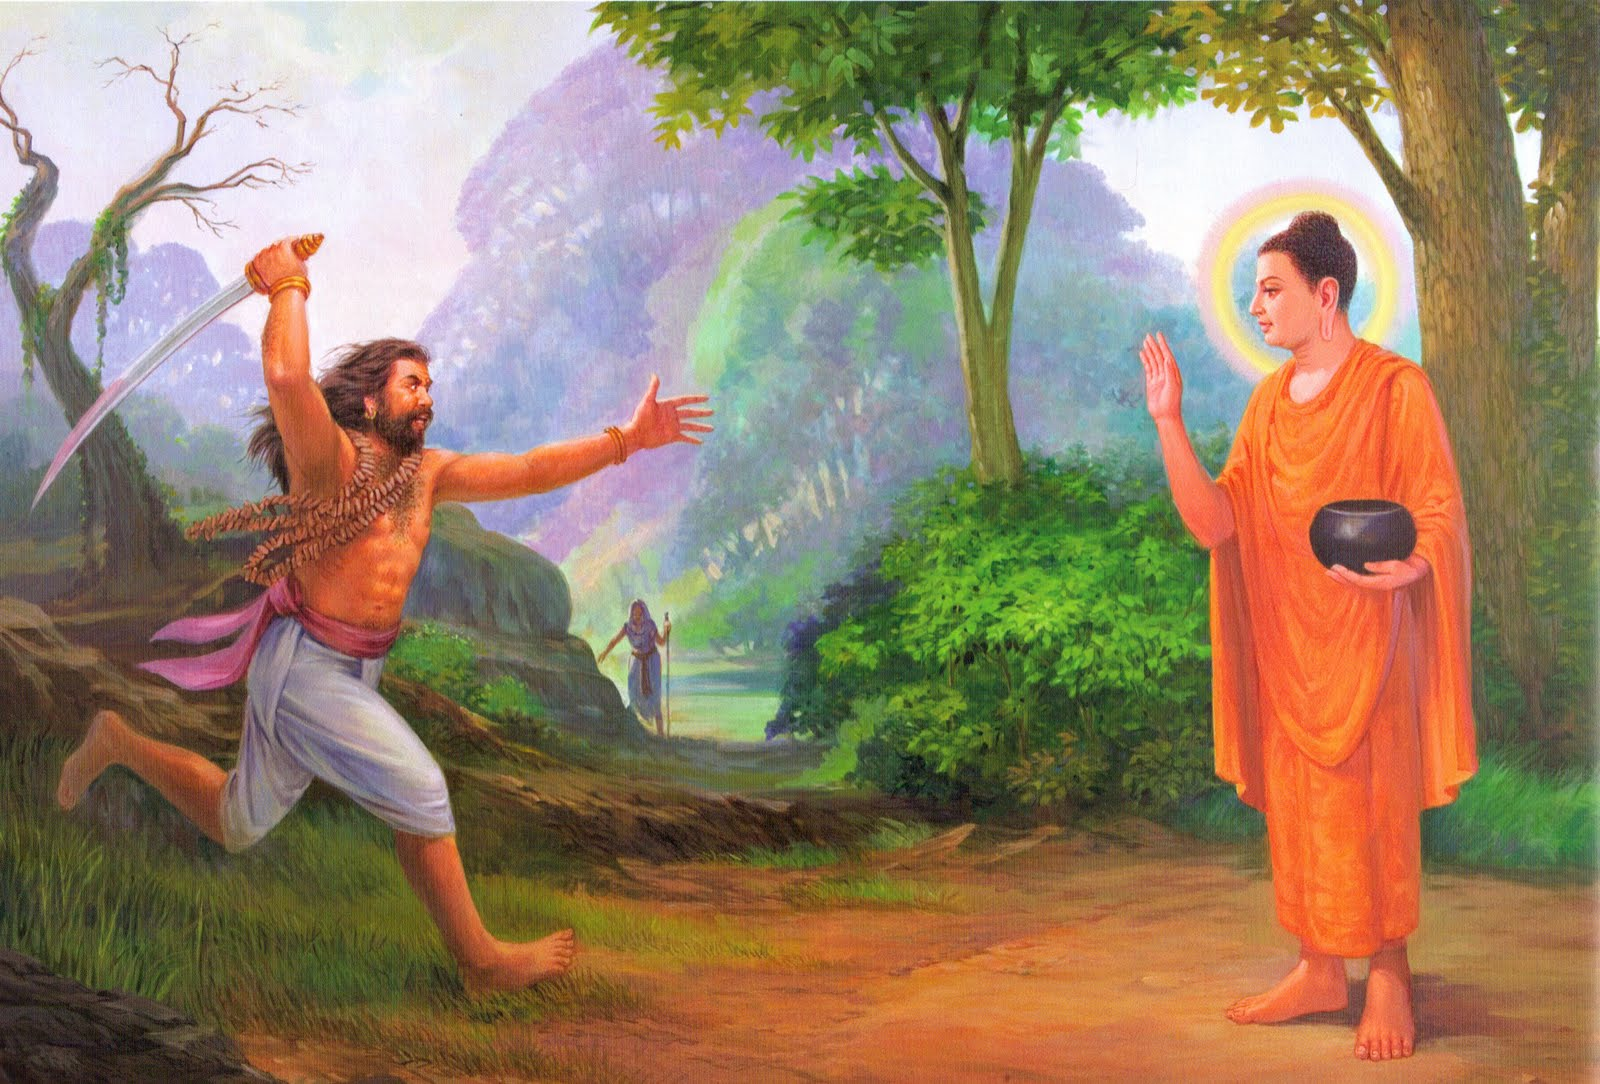
\includegraphics[width=0.8\linewidth]{./Diagrams/angulimala}
\caption{The story of Angulimāla, the killer tamed by the Buddha, is popular in Buddhist countries.}
\label{fig:angulimala}
\end{figure}

The Angulimāla Sutta gives an example of how past unwholesome kamma may be “watered down.”\footnote{MN 86: \url{http://www.accesstoinsight.org/tipitaka/mn/mn.086.than.html}} Before meeting the Buddha, Angulimāla was a serial killer. The story of how he was converted into an Arahat is also found in the Commentary.\footnote{\url{http://www.tipitaka.net/tipitaka/dhp/verseload.php?verse=173}} The following incident happened after Angulimāla had become an Arahat.

\begin{figure}[H]
\begin{quotation}
Then Venerable Angulimāla, early in the morning, having put on his robes and carrying his outer robe and bowl, went into Sāvatthī for alms. Now at that time a clod thrown by one person hit Venerable Angulimāla on the body, a stone thrown by another person hit him on the body, and a potsherd thrown by still another person hit him on the body. So Venerable Angulimāla – his head broken open and dripping with blood, his bowl broken, and his outer robe ripped to shreds – went to the Blessed One. The Blessed One saw him coming from afar and on seeing him said to him: “Bear with it, brahmin! Bear with it! The fruit of the kamma that would have burned you in Hell for many years, many hundreds of years, many thousands of years, you are now experiencing in the here-and-now!”
\end{quotation}
\caption{Extract of Angulimāla Sutta (MN 86).}
\label{fig:MN86}
\end{figure}

Obviously, Angulimāla had accumulated considerable unwholesome kamma from killing so many people before becoming a monk. Yet because of Angulimāla’s current condition of being an Arahat, the kammic result was reduced to some cuts and bruises. I think all of us have done some things in the past of which we are not proud. We should focus on creating wholesome conditions in the present; wholesome environment with many wholesome influences and keeping our precepts. And if by chance some past unwholesome kamma finds an opportunity to ripen, remember the Buddha’s words, “Bear with it!”

\subsection*{Completed Kamma}

\begin{figure}[H]

\begin{quote}

\tablesubheader{Killing}: \ding{172} A living being \ding{173} Knowledge \ding{174} Intention \ding{175} Effort \ding{176} Death

\tablesubheader{Stealing}: \ding{172} Property \ding{173} Knowledge \ding{174} Intention \ding{175} Effort \ding{176} Removal

\tablesubheader{Sexual Misconduct}: \ding{172} Forbidden partner (married / under guardianship) \ding{173} Intention \ding{174} Effort \ding{175} Acceptance

\tablesubheader{Lying}: \ding{172} Untrue thing \ding{173} Intention \ding{174} Effort \ding{175} Communication

\tablesubheader{Slander}: \ding{172} People to be separated \ding{173} Intention \ding{174} Effort \ding{175} Separation

\tablesubheader{Harsh Speech}: \ding{172} Person \ding{173} Intention \ding{174} Effort

\tablesubheader{Idle Talk}: \ding{172} Inclination toward idle talk \ding{173} Effort \ding{174} Others accept 

\tablesubheader{Covetousness}: \ding{172} Property \ding{173} Thought of “I wish it were mine”

\tablesubheader{Ill Will}: \ding{172} Another person \ding{173} Thought of “I hope that the other person is destroyed”

\tablesubheader{Wrong view}: \ding{172} Ideas of “no kamma”/“no cause”/“no cause and no result” \ding{173} Manifestation

\end{quote}

\caption{Conditions required to make kamma “completed.”}
\label{fig:Completed}
\end{figure}

Let’s now proceed to the topic of “Completed Kamma.” As mentioned in the previous lesson, “Completed Kamma” is sufficiently weighty to condition rebirth. For example, the kamma created when I enjoy my coffee is not weighty enough to condition rebirth. \textbf{Attachment} to my coffee still creates unwholesome kamma, but not the rebirth-linking kind of kamma.

The Buddha listed ten unwholesome actions that can cause rebirth in a woeful plane: killing, stealing, sexual misconduct, lying, slander, harsh speech, idle talk, coveting, ill will and \textbf{Wrong view}.\footnote{MN 41: \url{http://www.accesstoinsight.org/tipitaka/mn/mn.041.nymo.html\#unwholesome10}} According to the Commentary, for an unwholesome action to condition rebirth in a woeful plane, certain conditions must be met, and when all of these conditions are met, it is considered to be “completed kamma.” The Commentary also identifies the factors that, in addition to \textbf{Volition}, impact the weight of the kamma produced.\footnote{“The Expositor” (\textit{Atthasālinī}), pages 128--134.}

For killing, the required factors are: a living being (human or animal), knowledge that the being exists, intention to kill, effort to kill and consequential death. Killing a virtuous person is weightier than killing an immoral person, killing a human is weightier than killing an animal, killing a domesticated animal is weightier than killing a wild animal, killing a large animal is weightier than killing a small animal.\footnote{It requires a lot more effort (and thereby more intention) to kill a large animal as compared to killing a small animal such as a mosquito.}

The Commentary mentions\footnote{\url{http://www.tipitaka.net/tipitaka/dhp/verseload.php?verse=001}} a blind monk who inadvertently stepped on insects while doing walking meditation. The Buddha explained that the monk had done nothing wrong because there was no awareness of the existence of the insects and no intention to kill. 

\pagebreak

Buying meat at the grocery store or ordering meat from the menu of a restaurant are not killing, because there is no intention to have an animal killed specifically for you. On the other hand, it is considered killing if you order fresh seafood at a restaurant that keeps live seafood in tanks. The Buddha did allow monks to eat meat and fish, as long as the monk does not suspect that the meat or fish was killed for the purpose of feeding monks.\footnote{See Vinaya Volume 4, page 325. Also on page 298: Certain types of meat were not allowed under any circumstances: humans, horses and elephants (considered too noble to eat), dogs (considered to be too disgusting to eat), snakes, lions, tigers, leopards, bears and hyenas (there was a belief that eating one of these predators would give off a smell causing similar predators to attack the monk).}

There is a story in the Commentary of a female Sotāpanna who prepared weapons for her husband who was a hunter. The Buddha explained that she did not break the precept of avoiding killing because she was only preparing things for her husband.\footnote{\url{http://www.tipitaka.net/tipitaka/dhp/verseload.php?verse=124}}

Both the judge who issues a death sentence and the executioner who performs the act are guilty of killing. Suicide, euthanasia, mercy killing and abortion are all considered to be killing. There is no fault in killing plants, bacteria or germs because they do not have consciousness and are therefore not considered to be “living beings.”\footnote{Monks should not cut down plants (see Vinaya Volume 2, page 226 \url{http://www.accesstoinsight.org/tipitaka/vin/sv/bhikkhu-pati.html\#pc-11}); this is to avoid causing inconvenience to any \textit{Deva} who may be living there.}

For stealing, the required factors are: another’s property, knowledge that it is another’s property, intention to steal, effort to steal and removal of the property. Stealing from a virtuous person is weightier than stealing from an immoral person. Stealing a valuable object is weightier than stealing a worthless object.

The Commentary mentions that forgery or using false weights when conducting business is considered to be stealing. Personal use of the office photocopier or making personal phone calls during office hours is also stealing. Buying something in another country to avoid paying import duties in your home country is also stealing.\footnote{This is stealing from the government by illegally avoiding paying import duties. Buying things at the Duty Free shop is legally avoiding paying import duties, so this is not considered to be stealing.}

For sexual misconduct, the required factors are a woman who is forbidden, lustful intention, engaging in sexual intercourse and acceptance of the union. Sexual misconduct with a virtuous woman is weightier than with an immoral woman. A woman is forbidden if she is married, engaged, under the guardianship of a family member, a convict or a nun.

Adultery is sexual misconduct. A rapist is guilty of sexual misconduct but the victim of rape is not guilty because there was no acceptance of the union. Assuming that the factors are not met, the definition of sexual misconduct does not prohibit premarital sex,\footnote{At the time of the Buddha, people were married in their early teens, so premarital sex was not an issue.} homosexuality\footnote{The Suttas are silent on the subject of homosexuality among laypeople. Any form of sexual activity is prohibited for monastics.} or prostitution.\footnote{Associating with prostitutes is a cause of downfall (see Sn 1.6: \url{http://www.accesstoinsight.org/tipitaka/kn/snp/snp.1.06.nara.html}).}

For lying, the required factors are an untrue thing, intention to deceive, effort to deceive and communication of the untruth. The weightiness depends on the amount of welfare destroyed by the lie. Telling “white lies” to get children to behave, to close a business deal or insincere flattery are all lying. If an accountant conceals financial irregularities under instruction from their boss, both are lying.

\pagebreak

For slander, the required factors are people to be separated, intention to separate them, effort to separate them and separation. Slandering a virtuous person is weightier than slandering an immoral person.

For harsh speech, the required factors are a person to be abused, an angry thought and the abuse. Abusing a virtuous person is weightier than abusing an immoral person. 

Reminds me of a joke: before you criticize someone, walk a mile in his shoes. That way, if he gets angry, he’ll be a mile away and barefoot.

For idle talk, the required factors are an inclination toward useless topics of conversation such as politics, fashion or gossip,\footnote{The list of useless topics of conversation (\textit{tiracchānakathā}; literally “animal talk”) is found in AN 10.69 (\url{http://www.accesstoinsight.org/tipitaka/an/an10/an10.069.than.html}): “conversation about kings, robbers, ministers of state, armies, alarms, battles, food and drink, clothing, furniture, garlands, scents, relatives, vehicles, villages, towns, cities, the countryside, women and heroes, the gossip of the street and the well, tales of the dead, tales of diversity, the creation of the world and of the sea, talk of whether things exist or not.”} talking about useless topics and other’s accepting the conversation. Frequent indulgence in idle talk makes the kamma weightier. My personal view is that involvement in politics is not conducive to one’s spiritual development. In fact, monks are not allowed to vote in elections in Myanmar or Thailand.\footnote{Sri Lankan monks can vote and there is a political party led by monks: (\url{http://en.wikipedia.org/wiki/Jathika_Hela_Urumaya}).} 

Reminds me of a joke: four monks are meditating when a flag stars flapping. The first monk says, “Flag is flapping,” the second monk says, “Wind is flapping,” the third monk says, “Mind is flapping” and the fourth monk says “Mouths are flapping.”

For coveting, the required factors are another’s property and the thought, “I wish it were mine.” Coveting the property of a virtuous person is weightier than coveting the property of an immoral person. Coveting a valuable object is weightier than coveting a worthless object.

For ill will, the required factors are another person and the thought, “I hope that the other person is destroyed.” Harbouring ill will against a virtuous person is weightier than harbouring ill will against an immoral person. Merely disliking another person is not completed kamma unless there is the thought of “I wish that they were dead.”

For \textbf{Wrong view}, the required factor is the arising idea of “there is no kamma,” “there is no cause” or “there is no cause and no result.” Frequent \textbf{Wrong view} makes the kamma weightier. Denying kamma and thinking “there are no consequences” leads to a lack of moral responsibility.

\pagebreak

\subsection*{Classifications of kamma in the Commentary}

\begin{figure}[H]
\begin{quote}
\tablesubheader{By way of function}: \ding{172} Productive kamma \ding{173} Supportive kamma \ding{174} Obstructive kamma \ding{175} Destructive kamma

\tablesubheader{By time of ripening}: \ding{172} Immediately effective kamma \ding{173} Subsequently effective kamma \ding{174} Indefinitely effective kamma \ding{175} Defunct kamma

\tablesubheader{By order of ripening}: \ding{172} Weighty kamma \ding{173} Death proximate kamma \ding{174} Habitual kamma \ding{175} Reserve kamma

\tablesubheader{By place of ripening}: \ding{172} Unwholesome kamma \ding{173} Sense sphere wholesome kamma \ding{174} Fine material sphere kamma \ding{175} Immaterial sphere kamma

\end{quote}

\caption{Classifications of kamma in the Commentary: By way of function, by time of ripening, by order of ripening and by place of ripening.}
\label{fig:Classifications}
\end{figure}

\subsubsection*{Kamma by way of function}

The Commentary defines four types of kamma by way of function; productive kamma, supportive kamma, obstructive kamma and destructive kamma.

At the time of rebirth, productive kamma determines the new realm of existence and the new gender; things that do not change throughout the existence. During existence, productive kamma supports continued life of the body and produces other results.

Supportive and obstructive kamma arise during an existence, not at rebirth. Supportive and obstructive kamma do not produce its own results, but works to extend or diminish the functions of the productive kamma. For example, supportive kamma can extend our lifespan, just like healthy eating and exercise. Obstructive kamma can decrease our lifespan, just like junk food and an unhealthy lifestyle.

Destructive kamma cuts off and replaces the function of productive kamma. For example, destructive kamma can suddenly cut a life short, as in a fatal accident.

When discussing destructive kamma, I am often asked, “What is the role of kamma when there is an airplane crash and everybody on board dies?” The cause of the crash had nothing to do with kamma. Earthquakes, fires and airplane crashes are not caused by kamma. Kamma works at an individual level. A Sutta explains, “That kamma of yours was not done by your mother, not by your father, not done by your brother, sister, friends and companions, kinsmen and relatives, and not done by the \textit{Devas}. That kamma was done by you yourself, and you yourself will experience its result.”\footnote{MN 130: \url{http://www.accesstoinsight.org/tipitaka/mn/mn.130.than.html\#yama}} All of us, including all the people on the airplane, have had uncountable unwholesome intentions in past lives and in this life. Everybody is carrying with them past kamma that has the potential to arise as destructive kamma when supported by other conditions. So for each of the people on the airplane, the crash was a condition for their individual destructive kamma to arise and cut short their lifespan.

\pagebreak

\subsubsection*{Kamma by time of ripening}

The Commentary classifies kamma according to the time of ripening. As we will discuss during the next lesson on processes, seven identical kamma-creating Mind Moments arise in sequence as part of the sensing process and as part of the thinking process.

The first of the seven kamma-creating Mind Moments is the weakest.\footnote{It is weak because the previous Mind Moment is of a different type.} This creates “immediately effective kamma,” kamma that can ripen only in the current existence. If at the end of the current existence, this kamma has not found conditions to ripen, it becomes “defunct.”

The last of the seven kamma-creating Mind Moments is the second weakest.\footnote{It is weak because the subsequent Mind Moment is of a different type.} This creates “subsequently effective kamma,” kamma that can ripen only in the next existence. If at the end of the next existence, this kamma has not found conditions to ripen, it becomes “defunct.”

The middle five of the kamma-creating Mind Moments are strong.\footnote{They are strong because they are supported by presence of the same kind of Mind Moment both before and after their arising.} These Mind Moments create “indefinitely effective kamma” that can arise any time after the next existence. These kamma never become defunct as long as the round of rebirths continues.

\subsubsection*{Kamma by order of ripening}

The Commentary classifies rebirth-linking kamma according to the order of ripening at the moment of death. There are four classifications of rebirth-linking kamma: weighty kamma, death proximate kamma, habitual kamma and reserve kamma.

Weighty kamma will definitely ripen when death occurs. If one kills one’s mother, kills one’s father, kills an Arahat, wounds a Buddha or maliciously causes a split in the Sangha, then it is guaranteed that the next rebirth will be in Hell. If one maintains a jhāna until the moment of death, rebirth is guaranteed in the fine material plane or the immaterial plane, depending on the level of jhāna.\footnote{Visuddhimagga XIX.15 (see Footnote 2 for link).} 

If one attains jhāna during a retreat and goes back to the world without maintaining it, the jhāna attainment will not qualify as weighty kamma. If one develops the jhāna and later commits one of the five heinous crimes, the good kamma would be obliterated by the evil deed. For example, when Devadatta\footnote{\url{http://en.wikipedia.org/wiki/Devadatta}} wounded the Buddha and caused a split in the Sangha, he lost his psychic powers associated with jhāna and was guaranteed rebirth in Hell.\footnote{Devadatta lost his psychic power in Vinaya Volume 5, page 260 and was guaranteed to be reborn in \textit{Avīci} Hell in Vinaya Volume 5, page 271. Also see story from the Commentary: \url{http://www.tipitaka.net/tipitaka/dhp/verseload.php?verse=017}} If someone were first to commit one of the heinous crimes, they would not be able later to attain jhāna or sainthood because the evil kamma would create an insurmountable obstruction. 

For example, at the end of a discourse to King Ajātasattu, the Buddha said, “If he had not killed his father, the King could have attained sainthood while listening to that discourse.”\footnote{In the Theravāda version of the Sutta (DN 2: \url{http://www.accesstoinsight.org/tipitaka/dn/dn.02.0.than.html\#eye}), even the Buddha could not help King Ajātasattu escape the results of weighty kamma. In the Mahāyāna version of the Sutta, the simple act of meeting the Buddha reduces or eliminates the consequences of the King’s patricide. The concept of kamma evolved over time (see \url{http://blogs.dickinson.edu/buddhistethics/files/2014/01/Jayarava-Karma-final.pdf}).}

\pagebreak

It is highly unlikely that we will commit any of the five heinous deeds or die while in jhāna, so our most likely rebirth-linking kamma will be “death proximate kamma.” This is a strong thought that arises close to the time of death. I was fortunate to be at my mother’s bedside when she passed away. I kept reminding her of the many good things she had done during her life. I wanted her to die with wholesome thoughts. 

There is a story in the Commentary of an executioner who was reborn in heaven because he had just heard the Dhamma.\footnote{\url{http://www.tipitaka.net/tipitaka/dhp/verseload.php?verse=100}} In another story, a virtuous monk was reborn as a flea in his robe because he was attached to the robe.\footnote{\url{http://www.tipitaka.net/tipitaka/dhp/verseload.php?verse=240}} In yet another story, a queen who was a great supporter of the Buddha had an unfortunate rebirth because her last thought was of a single immoral act that she had done.\footnote{\url{http://www.tipitaka.net/tipitaka/dhp/verseload.php?verse=151}} On the surface, it may seem that the executioner, the virtuous monk and the queen were treated unfairly, but they still carried the kammic seeds from their previous deeds which would have an opportunity to arise later.\footnote{Countering the superficial understanding of kamma is one of the themes of MN 137: \url{http://www.accesstoinsight.org/tipitaka/mn/mn.136.than.html}}

If there is no strong “death proximate kamma,” then “habitual kamma” has an opportunity perform the function of rebirth-linking. As its name implies, “habitual kamma” arises from a repetitive action such as regularly meditating or regularly drinking alcohol.

Finally, if there is no weighty kamma, no strong death proximate kamma and no habitual kamma, then some random, reserve kamma can arise. This reserve kamma may even be from a previous life. 

For example, earlier I mentioned the virtuous monk who was reborn as a flea in his robe because of unwholesome “death proximate” kamma. After this monk died, the Buddha instructed the other monks not to touch the robe for seven days. This would ensure that the flea would not get upset, and the flea’s reserve kamma could then allow the flea to be reborn in heaven. 

I also mentioned the queen who had an unfortunate rebirth because of her last thought. When the queen died, the king decided to go to the Buddha to ask about her plane of rebirth. The Buddha distracted the king and he forgot to ask the question so he returned the next day. For seven days the Buddha caused the king to forget his question, but on the eighth day, the queen had been reborn in heaven because of the random kamma of her past good deeds. The Buddha then told the king that the queen had been reborn in heaven.

Here is an analogy to reflect the order of ripening of rebirth-linking kamma. Suppose that many cattle are kept in a shed for the night. In the morning the door of the shed is opened to let the cattle go to the pasture. Now which one will go first? If there is a leader among them whom everyone respects, this one will walk majestically to the door and go out first. This is weighty kamma. If there is no leader, the one nearest the door will go out first. This is death proximate kamma. Sometimes a vigilant one, which has regularly noticed the time when the shed is opened, may walk to the door just before it is opened and goes out first. This is habitual kamma. Sometimes an unexpected frail one, being pushed by stronger ones, may come out of the shed first. This is reserve kamma.

All this discussion about rebirth reminds me of two jokes: “I hear that rebirth is making a comeback.” and “I didn’t believe in rebirth during my last lifetime, either.”

\pagebreak

\subsubsection*{Kamma by place of ripening}

Finally, the Commentary classifies kamma according to the place of ripening. For rebirth-linking kamma, this means the place of rebirth, and for kamma arising during an existence, this means the planes of existence in which the kamma arises.

The Buddha referred\footnote{for example, MN 57: \url{http://www.accesstoinsight.org/tipitaka/mn/mn.057.nymo.html\#kammas4}} to four categories of kamma: dark kamma with dark ripening, bright kamma with bright ripening, dark-and-bright kamma with dark-and-bright ripening, and kamma that leads to the exhaustion of kamma. The first three categories correspond to place of ripening.

Dark kamma with dark ripening is unwholesome kamma resulting in rebirth in a Woeful State and suffering during existence in the Woeful State. Bright kamma with bright result is wholesome kamma resulting in rebirth in a \textit{Deva} realm and pleasant experiences during existence in the \textit{Deva} realm. Dark-and-bright kamma with dark-and-bright result is rebirth in a human realm with both unpleasant and pleasant experiences during existence. 

The fourth category of kamma according to the Suttas is “the kamma that leads to the exhaustion of kamma.” These are the actions leading to the Noble Eightfold Path. The ultimate destination of the Noble Eightfold Path is the Arahat, a being that does not create new kamma.

\subsection*{Kamma Causes}

\begin{figure}[H]

\begin{tabular*}{\textwidth}{L{\dimexpr0.4\textwidth-2\tabcolsep} | L{\dimexpr0.6\textwidth-2\tabcolsep}}
\toprule
\tableheader{Kamma Causes} & \tableheader{Kamma Results} \\
\midrule

Volition as part of past unwholesome Mind Moments (\textbf{1}--\textbf{12})

\vspace{2mm}

Volition as part of past wholesome Mind Moments (\textbf{31}--\textbf{38}, \textbf{55}--\textbf{59}, \textbf{70}--\textbf{73} and \textbf{82}--\textbf{85})
&
Plane of rebirth (Hell, animal, human, \textit{Deva}, etc.)

\vspace{2mm}

Mind Moments that process sense objects (\textbf{13}--\textbf{27})

\vspace{2mm}

Fruit Mind Moments (\textbf{86}--\textbf{89})

\vspace{2mm}

Body-sensitivity group, Heart-base group, Gender
\vspace{2mm}

Vital-nonad group and remaining sense-sensitivity groups (eye, ear, nose, tongue)
 \\
 
\bottomrule
\end{tabular*}
\caption{Causes and results of kamma.}
\label{fig:Kamma}
\end{figure}

Now look at the causes and results of both kamma and natural decisive support,\footnote{In the Abhidhamma, these are called “conditioning states” and “conditioned states.” In the context of kamma condition and natural decisive support condition, the simple terms “causes” and “results” make sense, but this is not the case for other types of conditioning forces.} according to the Abhidhamma.

According to the Abhidhamma, the cause of kamma is the Mental Factor of \textbf{Volition} when it arises as part of the Mind Moments that create new kamma. Referring to Figure \ref{Handout3}, the Mind Moments that create new kamma are in the top row and include Mind Moments \textbf{1}--\textbf{12}, Mind Moments \textbf{31}--\textbf{38}, Mind Moments \textbf{55}--\textbf{59}, Mind Moments \textbf{70}--\textbf{73} and Mind Moments \textbf{82}--\textbf{85}.

Mind Moments \textbf{1}--\textbf{12} create new unwholesome kamma and take sense objects or ideas as their object. The remaining Mind Moments in the top row of Figure \ref{Handout3} all create new wholesome kamma. Mind Moments \textbf{31}--\textbf{38} take sense objects or ideas as their object. Mind Moments \textbf{55}--\textbf{59} and Mind Moments \textbf{70}--\textbf{73} are the attainment of jhāna and Mind Moments \textbf{82}--\textbf{85} are the attainment of sainthood.

\subsection*{Kamma Results}

According to the Abhidhamma, the result of kamma is both mind and matter. Let’s start by looking at mind in a bit more detail. Mind is the Mind Moments in the middle row of Figure \ref{Handout3}. Whereas the Mind Moments involved in creating new kamma are “active,” the Mind Moments that are the result of past kamma are “passive.”\footnote{This is “Kamma result condition” (\textit{vipāka-paccaya}); see Chapter 12 of “The Conditionality of Life” (see Footnote 2 for link).}

At the time of rebirth, the rebirth-linking kamma from the previous existence results in a Life-continuum Mind Moment for the new existence. When the mind is not sensing or thinking, countless Life-continuum Mind Moments arise and fall away in succession. Each of these Life-continuum Mind Moments are the result of the same rebirth-linking kamma from the previous existence.

Let’s quickly recap what was discussed in the previous lesson regarding rebirth-linking kamma from the previous existence, the Life-continuum Mind Moment for the new existence and the plane of rebirth.

If the rebirth-linking kamma from the previous existence is unwholesome, the Life-continuum Mind Moment in the new existence will be Mind Moment \textbf{19}, and rebirth will happen in Realm \textit{1}--\textit{4}, the Woeful States. 

If the rebirth-linking kamma from the previous existence is two-rooted inferior kamma,\footnote{“Two-rooted” means rebirth-linking kamma created by Mind Moments \textbf{33}, \textbf{34}, \textbf{37} or \textbf{38}. “Inferior” means not having support (from other wholesome Mind Moments) before and after.} then the Life-continuum Mind Moment in the new existence will be Mind Moment \textbf{27} and rebirth will happen in the human realm.\footnote{These humans are congenitally disabled (blind or deaf from time of conception).}

If the rebirth-linking kamma from the previous existence is two-rooted superior kamma or three-rooted inferior kamma, then the Life-continuum Mind Moment in the new existence will be Mind Moment \textbf{41}, \textbf{42}, \textbf{45} or \textbf{46}\footnote{Mind Moments \textbf{41}, \textbf{42}, \textbf{45} and \textbf{46} have two roots (only \textit{alobha} and \textit{adosa}, no \textit{paññā}). Beings having Life-continuum with two roots cannot achieve jhāna or sainthood.} and rebirth will happen in the human realm or Realm \textit{6}. 

If the rebirth-linking kamma from the previous existence is three-rooted superior kamma,\footnote{“Three-rooted” means rebirth-linking kamma created by Mind Moments \textbf{31}, \textbf{32}, \textbf{35} or \textbf{36}. “Superior” means having support (from other wholesome Mind Moments) before and after.} the Life-continuum Mind Moment in the new existence will be Mind Moment \textbf{39}, \textbf{40}, \textbf{43} or \textbf{44}\footnote{Mind Moments \textbf{39}, \textbf{40}, \textbf{43} and \textbf{44} have three roots (\textit{alobha}, \textit{adosa} and \textit{paññā}). Beings having Life-continuum with three roots are able to achieve jhāna and sainthood.} and rebirth will happen in the human realm or a \textit{Deva} Realm, Realm \textit{6}--\textit{11}.

If the rebirth-linking kamma from the previous existence is the attainment of jhāna, Mind Moments \textbf{55}--\textbf{59} or Mind Moments \textbf{70}--\textbf{73}, then the Life-continuum Mind Moment in the new existence will be Mind Moment \textbf{60}--\textbf{64} or Mind Moment \textbf{74}--\textbf{77} and rebirth will happen in Realms \textit{12}--\textit{31}.

Now let’s discuss how past kamma can cause a result during the course of the present existence. This is through Mind Moments \textbf{13}--\textbf{27}, which process sense objects.

Imagine that a smell arises. As mentioned during our discussion of \textit{rūpa}, a smell may be intrinsically undesirable, such as the smell of garbage or intrinsically desirable such as the smell of coffee. The intrinsic nature of a smell has nothing to do with kamma. In other words, it is not because of kamma that garbage smells bad and coffee smells good.

\pagebreak

When a smell makes contact with the nose, this is a condition for nose-consciousness to arise. If the smell is intrinsically undesirable, such as garbage, then Mind Moment \textbf{15} arises, the result of past unwholesome kamma. If the smell is intrinsically desirable, such as coffee, then Mind Moment \textbf{22} arises, the result of past wholesome kamma.

There is no difference between Mind Moment \textbf{15} and Mind Moment \textbf{22} other than the type of kamma that caused them to arise and the intrinsic nature of the object they experience. Both Mind Moment \textbf{15} and Mind Moment \textbf{22} are rootless, ethically-neutral, and both Mind Moments include only the seven universal ethically-variable Mental Factors of \textbf{Contact}, \textbf{Feeling}, \textbf{Perception}, \textbf{Volition},\footnote{As mentioned earlier, in this kind of Mind Moment, the function of \textbf{Volition} is only to coordinate the activities of the other Mental Factors; \textbf{Volition} does not create new kamma.} \textbf{One-pointedness}, \textbf{Attention} and \textbf{Life faculty}.

We used an example of smelling, but the same principles holds for all of the sense-consciousness Mind Moments; those responsible for the bare act of seeing, hearing, smelling, tasting and body tactile sensation. In other words, intrinsically undesirable sense objects are captured by Mind Moments \textbf{13}--\textbf{17} and intrinsically desirable sense objects are captured by Mind Moments \textbf{20}--\textbf{24}.

Once an intrinsically undesirable sense object has been captured by Mind Moments \textbf{13}--\textbf{17}, the sense object is processed by Mind Moment \textbf{18} and Mind Moment \textbf{19}. The function of these two Mind Moments will be discussed in the next lesson. They are the result of the same past unwholesome kamma as the sense-consciousness that captured the sense object (Mind Moments \textbf{13}--\textbf{17}).

Similarly, once an intrinsically desirable sense object has been captured by Mind Moments \textbf{20}--\textbf{24}, the sense object is processed by Mind Moment \textbf{25} and either Mind Moment \textbf{26} or Mind Moment \textbf{27}. The function of Mind Moments \textbf{25}, \textbf{26} and \textbf{27} will be discussed in the next lesson. They are the result of the same past wholesome kamma as the sense-consciousness that captured the sense object (Mind Moments \textbf{20}--\textbf{24}).

Imagine that I step on a nail. The existence of the nail has nothing to do with kamma. The fact that I stepped on the nail has nothing to do with kamma. The stepping on the nail is a condition for some past unwholesome kamma to ripen and Mind Moment \textbf{17}; body-consciousness with painful \textbf{Feeling} arises. Mind Moment \textbf{18} and Mind Moment \textbf{19} will process this sense-object and then a decision needs to be made about how to react. Using the “Decision box” from Figure \ref{fig:Room}, it is time for a decision to be made. The decision will be made by Mind Moment \textbf{29} which has nothing to do with kamma. The point that I am making here is that, just as the Buddha said in the Salt Crystal Sutta, when kamma ripens in the here-and-now, it appears barely for a moment.

There is one more way in which past kamma has a mental result during the course of the present existence. Mind Moment \textbf{86} to Mind Moment \textbf{89} are the kammic result of Mind Moment \textbf{82} to Mind Moment \textbf{85}. For example, Mind Moment \textbf{82} is the “change of lineage,” the transition from worldling to Sotāpanna, the “Sotāpanna path” Mind Moment. A Sotāpanna can experience the “bliss of \textit{Nibbāna}” during the course of the present existence through experiencing Mind Moment \textbf{86}, the Sotāpanna fruit.

Let's look at how matter can be a result of past kamma. At the moment of rebirth, the same rebirth-linking kamma from the previous existence that resulted in the Life-continuum Mind Moment in the new existence also results in three groups of \textit{rūpas}. These three kamma-born groups are: the body-sensitivity group, the heart-base group that supports the Mind Moment and either the femininity group or masculinity group.

\pagebreak

At a suitable time after conception, the rebirth-linking kamma from the previous existence supports the arising of the vital-nonad group and the remaining sense-sensitivity groups: the \textbf{Eye-sensitivity} group, the \textbf{Ear-sensitivity} group, the \textbf{Nose-sensitivity} group and the \textbf{Tongue-sensitivity} group.

Throughout the course of existence, the rebirth-linking kamma from the previous existence will continue to support the arising of the vital-nonad group, the Heart-base group, either the femininity group or the masculinity group and the five sense-sensitivity groups.

The Buddha referred\footnote{SN 35.145: \url{http://www.accesstoinsight.org/tipitaka/sn/sn35/sn35.145.than.html}} to the six sense bases (eye-base, ear-base, nose-base, tongue-base, body-base and mind-base) as ‘old kamma’ because the five sense-sensitivity groups and the Heart-base group (that supports the mind) arise because of the rebirth-linking kamma from the previous existence. In the same Sutta, the Buddha referred to the mind’s reaction to what is sensed as ``new kamma.'' So ``new kamma'' includes Mind Moments \textbf{1}--\textbf{12} and Mind Moments \textbf{31}--\textbf{38}.

\subsection*{Natural Decisive Support Causes}

\begin{figure}[H]
\begin{tabular*}{\textwidth}{L{\dimexpr0.4\textwidth-2\tabcolsep} | L{\dimexpr0.6\textwidth-2\tabcolsep}}
\toprule
\tableheader{Natural Decisive Support Causes} & \tableheader{Natural Decisive Support Results} \\
\midrule

Past “strong” experiences:
\begin{itemize}
\item Mind Moments
\item Rūpa
\item Concepts
\end{itemize}

&
All current Mind Moments:
\begin{itemize}
\item Life-continuum Mind Moments
\item Mind Moments that process sense objects (\textbf{13}--\textbf{27})
\item Mind Moment that decides reaction (\textbf{29})
\item Mind Moments that create new kamma, including strength of volition (weightiness of kamma)\vspace*{-\baselineskip}
\end{itemize}

\\

\bottomrule

\end{tabular*}
\caption{Causes and results of natural decisive support.}
\label{fig:NDS}
\end{figure}

Let’s move on to natural decisive support condition. A simple way of explaining natural decisive support condition is to say that strong experiences in the past leave an impression that impacts the current Mind Moment. We use various expressions to describe this effect such as the impact of defilements, \textit{pārami}, accumulations, habits, vows, tendencies, the environment, your mood or recent events. All of these are different ways of describing the same thing; strong experiences in the past leave an impression that impact the current Mind Moment.

The cause of Natural Decisive Support is a strong experience in the past. This includes Mind Moments (which is consciousness and Mental Factors), \textit{rūpas} and even concepts. In other words, almost anything can be the cause of Natural Decisive Support, as long as it is “strong.”

In order to qualify as a cause for natural decisive support, the past experience must be “strong.” The Commentaries do not explain this aspect in much detail, so I will share with you my opinions about three ways in which an experience can be made “strong.”

\pagebreak

One way that an experience can be “strong” is through repetition. If something is repeated many times, it is reinforced and becomes “strong.” More than 10 years ago, a ground-breaking study\footnote{\url{http://www.investigatinghealthyminds.org/ScientificPublications/2003/DavidsonAlterationsPsychosomaticMedicine.pdf}} was done in the US. A group of office workers had their “happiness level” measured using an EEG, and their “healthiness level” measured by looking at their immune system response to a flu vaccine. Some of the office workers underwent an eight-week training program in \textbf{Mindfulness} meditation and some did not. Not surprisingly, the meditators were measurably happier and healthier after the \textbf{Mindfulness} program as compared to the non-meditators. The meditators then stopped meditating and four months later, EEG and blood tests were taken again. Even though the meditators had not meditated for four months, they were still measurably happier and healthier than the non-meditators. In other words, the strong experience acquired through the brief exposure to repeated \textbf{Mindfulness} meditation had a measurable effect on Mind Moments four months in the future. The mind and the health of the body are intimately connected, so the present happy Mind Moments contributed to a healthier body.

A second way that an experience can be “strong” is through being recent. A few years ago, driving home after a session of loving-kindness meditation, I stopped at a red light. When the light turned green, the car behind me accelerated and hit my rear bumper. The other driver and I both got out of our cars. I looked at my bumper and with a big smile on my face said, “No damage, no problem, have a wonderful day!” The other driver was shocked at my reaction because she expected to be scolded. If I had just finished a bad day at work, perhaps I would have scolded the other driver, but my reaction at that time was conditioned based on the recent loving kindness meditation.

A third way that an experience can be “strong” is through strong \textbf{Volition}. For example, a sincere vow has strong \textbf{Volition} and can influence future Mind Moments. Vows (especially the Bodhisattva vow)\footnote{\url{http://en.wikipedia.org/wiki/Bodhisattva_vow}} play an important role in many Mahāyāna traditions. A famous example from the Theravāda tradition is the vow taken aeons ago by the hermit Sumedha to become a future Buddha.\footnote{Detailed in the Buddhavamsa: \url{http://en.wikipedia.org/wiki/Buddhavamsa}} The Commentaries give the background history of the Buddha’s main disciples,\footnote{\url{http://www.wisdompubs.org/sites/default/files/preview/Great-Disciples-of-the-Buddha-Preview.pdf}} and these stories usually involve taking a vow in a previous life to become closely associated with a future Buddha.

When the definition of natural decisive support condition says that the causes are from the past, this includes previous lives. For example, while he was imprisoned, Nehru, the first Prime Minister of India, took great inspiration and strength from a picture of a Buddha statue.\footnote{\url{http://www.asiantribune.com/news/2003/10/19/image-buddha-even-inspired-nehru-sinha}} This is an example of a concept being a past cause through which natural decisive support impacted the current Mind Moment. Nehru was a Hindu, but I suspect that in a previous life, he may have been a Buddhist and this is why the picture could have such a strong effect on him. 

\pagebreak

As a teenager, after reading the Bible, I spent long periods in deep reflection asking myself, “What do I believe?” I was later shocked to discover that many of my personal beliefs were strongly aligned with Buddhism, because I had never been exposed to Buddhism. I could not believe that independently, I could arrive at the same beliefs as one of the world’s major religions. Later, I realized that I must have been a Buddhist in a previous life and when the mind was allowed to “go back to its roots” through deep reflection, I was able to reconnect with those beliefs through natural decisive support condition.

\subsection*{Natural Decisive Support Results}

Now let’s turn our attention to the results of natural decisive support condition. All current Mind Moments are impacted by natural decisive support. Whereas kamma condition only impacts the middle row of Figure \ref{Handout3}, natural decisive support condition impacts all 89 Mind Moments.

According to the Commentaries,\footnote{Visuddhimagga XVII.177 and XVII.270 (see Footnote 2 for link).} rebirth is conditioned by both kamma and natural decisive support. They also work together when conditioning the Mind Moments that process sense objects (Mind Moments \textbf{13}--\textbf{27}). Kamma may cause these types of Mind Moments to arise, but it is natural decisive support that impacts the intensity of the Mental Factors involved in the Mind Moment.

Once a sense object has been processed or an idea is present, then Mind Moment \textbf{29} has the function of determining the reaction. In the ``decision box" from Figure \ref{fig:Room}, it is the “decision making” Mind Moment. Mind Moment \textbf{29} is unrelated to kamma, but it is influenced by natural decisive support. It is because of natural decisive support condition that the mind flows to either the Danger Zone or to the Faultless Zone.

When a Mind Moment that creates new kamma arises, the Mind Moments in the top row of Figure \ref{Handout3}, it is natural decisive support that determines the intensity of the Mental Factors. For example, \textbf{Attachment} has many grades, ranging from simply enjoying my morning coffee to lustful passion. It is natural decisive support that determines the intensity of the \textbf{Attachment} and the intensity of all of the other Mental Factors.

\subsection*{Implications of Natural Decisive Support}

\begin{figure}[H]
\begin{quotation}
Natural Decisive Support is how the current Mind Moment is impacted by accumulations, habits, defilements, \textit{pārami}, vows, tendencies, the environment, your mood or recent events.

Don’t try to control the mind, train the mind by creating “strong” experiences through:

\begin{itemize}

\item Repeated wholesome volition (dāna, precepts, meditation, studying the Dhamma, wise attention, etc.)

\item Associating with good friends in the dhamma (\textit{kalyāṇa-mitta})

\item Suitable environment, suitable food

\end{itemize}
\end{quotation}
\caption{Implications of natural decisive support.}
\label{fig:Implications}
\end{figure}

Clearly, natural decisive support condition plays an important role in how the mind operates. The ways in which experiences are made “strong” (repetition, being recent and through strong \textbf{Volition}), suggest strategies that we can apply as part of spiritual development.

Spiritual development is a process of training the mind. Training the mind is like any type of training. It is not a “control” paradigm but a method of “working with the mind.” As I mentioned in the first lesson, the mind is like a little puppy dog; it cannot be controlled but it can be trained. The Buddha laid out a gradual training for monks\footnote{MN 107: \url{http://www.accesstoinsight.org/tipitaka/mn/mn.107.horn.html}} and the precepts are “rules of training.” If we want to develop ourselves spiritually, we need to put a training program in place. This training program may include regularly offering \textit{dāna}, regularly taking precepts and regular meditation. Strong \textbf{Volition} can increase the strength of an experience and increase its impact, so it is better to put our hearts into our spiritual training.

The Buddha also advised\footnote{Sn 2.4: \url{http://www.accesstoinsight.org/tipitaka/kn/snp/snp.2.04.nara.html}} us not to associate with fools, but to associate with the wise. This is because the people with whom we regularly associate have a significant impact on how we think. Associating with wise people and good friends in the dhamma (\textit{kalyāṇa-mitta}) supports the development of discretion, the ability to see clearly what is right and what is wrong.

We should also remember that things such as the weather, the food that we have eaten and recent events in our lives can also impact how the mind thinks. It is often better to delay making important decisions to make sure that our judgement is not clouded by what has happened recently.

\pagebreak

\subsection*{Summary of Key Points}

\begin{itemize}

\item “It is \textbf{Volition} (\textit{cetanā}) that I call kamma. For having willed, one acts by body speech or mind.”

\item Everything arises because of multiple conditions; kamma is only one of the factors.

\begin{itemize}

\item Living in a wholesome environment with many wholesome influences and keeping the precepts creates conditions for wholesome kamma-seeds to ripen.

\end{itemize}

\item “Beings are owners of their kamma, heirs of their kamma; they originate from their kamma, are bound to their kamma and have their kamma as their refuge.”

\item Unwholesome intention can result in rebirth in the Woeful Planes or can result in unfortunate circumstances if reborn as human.

\item Ten things that can cause rebirth in a woeful plane: killing, stealing, sexual misconduct, lying, slander, harsh speech, idle talk, coveting, ill will and \textbf{Wrong view}.

\item Four classifications of rebirth-linking kamma: weighty kamma, death proximate kamma, habitual kamma and reserve kamma.

\item The cause of kamma is the Mental Factor of intention in the Mind Moments shown in the top row of Figure \ref{Handout3}.

\item The results of kamma are Mental Factors in the middle row of Figure \ref{Handout3} and also the kamma-born groups of \textit{rūpas}.

\item Because of natural decisive support, “strong” past experiences leave impressions that impact the current Mind Moment.

\begin{itemize}

\item We use various expressions to describe this effect, such as the impact of defilements, \textit{pārami}, accumulations, habits, vows, tendencies, the environment, your mood or recent events.

\end{itemize}

\item Experiences can be “strong” due to repetition, being recent or strong \textbf{Volition}.

\item All current Mind Moments and the intensity of Mental Factors within the current Mind Moment are influenced by natural decisive support.

\begin{itemize}

\item Rebirth is conditioned by both kamma and natural decisive support.

\end{itemize}

\item Implications of natural decisive support are that we should:

\begin{itemize}

\item Approach spiritual development with a “training” paradigm (new approach), not with a “control” paradigm (traditional approach).

\item Associate with the wise and not associate with fools.

\item Be aware of the effects that the environment (including food) has on our mind.

\end{itemize}

\end{itemize}

In my opinion, the most important thing to remember about kamma is that we should not worry about our past unwholesome kamma. We should focus on creating an environment that allows past wholesome kamma to ripen and conduces to the creation of new wholesome kamma. Finally, the most important thing to remember about natural decisive support is that the mind cannot be controlled, but it can be trained to strengthen good habits.

\newpage

\subsection*{Questions \& Answers}

\question{Kamma comes from the underlying intention, not from what is said or done. However, Paritta chanting is supposed to bring protection. Please clarify.}

The Ratana Sutta\footnote{Sn 2.1: \url{http://www.accesstoinsight.org/tipitaka/kn/snp/snp.2.01.than.html}} is a good example of a \textit{Paritta}. In this Sutta, the Buddha addresses the \textit{Deva} saying, “Spirits, you should all be attentive. Show kindness to the human race. Day and night they give offerings, so being heedful, protect them.” The city of Vesālī was experiencing famine and epidemic\footnote{\url{http://www.tipitaka.net/tipitaka/dhp/verseload.php?verse=290}} and the Buddha recited this Sutta to ask the \textit{Deva} to protect the humans in Vesālī. This suggests that the \textit{Deva} may be able to influence environmental factors.

The Commentary explains\footnote{“The Questions of King Milinda” (\textit{Milindapañha}), 150f} that \textit{Paritta} chanting works only for certain individuals. A \textit{Paritta} can fail due to lack of faith, due to counter-effect of defilements or due to kamma. In other words, \textit{Paritta} are only effective for those who deserve to be protected.

The power of a \textit{Paritta} comes not so much from the words as from the strength of the intention, or \textbf{Volition} in the mind, as the \textit{Paritta} is recited.

\question{How can I help someone who is critically ill?\footnote{Extracted from: \url{http://www.buddhanet.net/pdf_file/buddhist_funeral.pdf}}}

The best way to help someone who is dying is to encourage them to have a positive, peaceful mind that is free of disturbing emotions such as fear, anger, \textbf{Attachment}, depression, etc. To do this, we need to work first on our own state of mind. If we have disturbing emotions regarding death, it will be very difficult to help another person overcome theirs. Clinging to emotions will cause both our mind and the mind of the dying to be disturbed. Be calm, kind, sensitive and supportive, avoiding strong emotional reactions. The dying person should be encouraged to accept death as a natural and inevitable phenomenon. Assure the dying person that they need not worry about their family.

If the dying person belongs to another religion, encourage them to have faith, to pray, to have positive thoughts, etc. in accordance with their religious beliefs and practices. Do not try to impose your own beliefs as this may give rise to confusion, disturbing emotions or negative thoughts in the mind of the dying.

If the dying person is Buddhist or not, remind them repeatedly about the good deeds that they have done during their lives. This will lead to positive, wholesome thoughts and will be especially meaningful to a Buddhist who appreciates the law of kamma.

If the dying person is a Buddhist, you can place a Buddha statue close by, invite them to take the three refuges, invite monks to chant blessings\footnote{\url{ http://en.wikipedia.org/wiki/Paritta}} or inform them of good deeds such as charity done in their name. If the dying person is a Buddhist meditator, you can remind them of their meditation  practice.

\pagebreak

\question{What is the Theravāda view on vegetarianism?}

At one point, Devadatta proposed that monks should follow five austerities:\footnote{See Vinaya Volume 5, page 276.}

\begin{itemize}
\item Monks should dwell all their lives in the forest.
\item Monks should live entirely on alms obtained by begging (accept no invitations to meals).
\item Monks should wear only robes made of discarded rags and accept no robes from the laity.
\item Monks should dwell at the foot of a tree and not under a roof.
\item Monks should abstain completely from fish and flesh (be vegetarian).
\end{itemize}

The Buddha said these practices were optional for a monk (except that of sleeping under a tree during the rainy season); they are among the 13 ascetic practices.\footnote{See Visuddhimagga II.2 (see Footnote 2 for link).} So the Theravāda view is that vegetarianism is optional for monks and by extension for laypeople (personally, I am vegetarian). The following site has a concise summary of the Theravāda view: \url{http://www.urbandharma.org/udharma3/vegi.html}. 

A late addition to a Mahāyāna Sutra (\url{http://en.wikipedia.org/wiki/Lankavatara_Sutra}) justifies vegetarianism as follows:

\begin{itemize}
\item Present-day animals may have been one’s kin in the past.
\item One’s own parents and relatives may in a future life be born as an animal.
\item There is no logic in exempting the meat of some animals on customary grounds while not exempting all meat.
\item Meat is impure as it is always contaminated by body wastes.
\item The prospect of being killed spreads terror amongst animals.
\item All meat is nothing other than carrion (decaying flesh or like road-kill in modern terms).
\item Meat eating makes the consumer cruel and sensual.
\item Man is not a carnivore by nature.
\end{itemize}

I have heard the argument that eating meat is indirectly breaking the precept of not killing. I do not consider ``indirect kamma" to be a valid argument. While it is true that for me to eat meat, somebody had to kill an animal, I do not believe that I ``inherit" the unwholesome kamma from this person. The Suttas clearly state that one experiences the results of one's own actions, not the actions of others.\footnote{MN 130: \url{http://www.accesstoinsight.org/tipitaka/mn/mn.130.than.html\#yama}}


%\section{Processes}

Welcome to the final lesson of this Practical Abhidhamma Course.\footnote{See Chapter 4 of “A Comprehensive Manual of Abhidhamma” (see Footnote 2 for link). \newline Also see \url{http://host.pariyatti.org/treasures/Process_of_Consciousness_and_Matter.pdf}} This lesson covers processes including the sensing process, thinking process and rebirth process.\footnote{The Abhidhammattha Sangaha also describes processes involved in attaining jhāna and attaining sainthood, but I have not included them as this is a “practical” course.} In other words, I will describe how there is seeing without a seer, how there is thinking without a thinker and how there is rebirth without a Self. From an Abhidhamma perspective, these processes involve a sequence of Mind Moments arising in a defined order.

\subsection*{Importance of guarding the senses}

Let's start with the importance of guarding the senses.\footnote{For more information on guarding the senses, see Visuddhimagga I.50--59 (see Footnote 2 for link).}

A Buddhist scholar wrote, “Where would I possibly find enough leather with which to cover the surface of the earth? Just the leather on the soles of my shoes is equivalent to covering the earth with it. Likewise, it is not possible for me to restrain the external course of things, but should I restrain my own mind, what would be the need to restrain all else?”\footnote{Śāntideva (\url{http://en.wikipedia.org/wiki/Shantideva}) in his “Bodhisattvacaryāvatāra” (A Guide to the Bodhisattva’s Way of Life): \url{http://en.wikipedia.org/wiki/Bodhisattvacaryavatara}} In other words, it is not possible to see only nice things, hear only nice sounds, etc. The path of life is littered with sharp objects. Guarding the six senses does not change the nature of the world but it does offer protection to the mind.

In the Commentary, a senior monk receives instruction from a seven-year-old Arahat as follows, “To catch a lizard that has entered an ant-hill with six holes, one would cover five holes and keep watch at the sixth. Thus one should close the five senses, and watch the mind.”\footnote{\url{http://www.tipitaka.net/tipitaka/dhp/verseload.php?verse=282}; the instructions given by the seven-year-old Arahat to Poṭṭhila Thera are not included in the on-line translation, but are part of the Pāḷi original.}

The mind is the most difficult sense to guard because the mind loves to attach itself to things. Imagine that I ask you to hold up a cup. Initially, it is no problem but after a while the cup starts to feel heavy. If you were able to put the cup down for a short time, the muscles in your arm would be refreshed and you could easily pick up the cup again. The cup represents the thoughts that obsess the mind. If the mind could let go of these things, even for a short time, the mind would be refreshed.

The Buddha had a gradual seven-step path to train monks, with each step building on the previous steps.\footnote{MN 107: \url{http://www.accesstoinsight.org/tipitaka/mn/mn.107.horn.html}} The first step is morality, the second step is guarding the senses, the third step is moderation with food, the fourth is wakefulness, the fifth is \textbf{Mindfulness} of activities, the sixth is removing of the hindrances and the seventh step is attainment of the jhānas. In other words, guarding the senses is a very basic training for monks and for anybody looking to develop themselves spiritually. The Buddha warned, “On seeing a form with the eye, he does not grasp at its signs and features\footnote{“Signs and features” are the distinctive qualities of the object that can trigger latent defilements.} since if he left the eye-faculty unguarded, evil unwholesome states might invade him.”\footnote{Also found in MN 27: \url{http://www.accesstoinsight.org/tipitaka/mn/mn.027.than.html}}

\pagebreak

The goal of spiritual development is to purify the mind. Purifying the mind involves guarding the senses so that impurities don’t get a chance to arise. When sense-objects are recognized, accepted, depersonalized and seen as they truly are, there are no conditions to support the arising of impurities and as a result, the mind is purified.\footnote{\textit{\textbf{R}}ecognize, \textbf{\textit{A}}ccept, \textit{\textbf{D}}epersonalize, \textbf{\textit{I}}nvestigate, \textit{\textbf{C}}ontemplate \textbf{\textit{A}}\textit{nicca}/\textit{\textbf{C}}ontemplate \textbf{\textit{A}}\textit{nattā}, \textbf{\textit{L}}et go \\(the \textit{\textbf{RADICAL}} approach).}

The Buddha explained the reason laypeople fight with other laypeople is \textbf{Attachment} to sense pleasures, addiction to sense pleasures and obsession with sense pleasures.\footnote{AN 2.37: \url{http://obo.genaud.net/dhamma-vinaya/pts/an/02_twos/an02.031-040.wood.pts.htm}\\(see section [36]).} In other words, inability to guard the senses is the root cause of conflict, from marital squabbles to wars between countries. In the same Sutta, the Buddha explained the reason one ascetic fights with other ascetics is \textbf{Attachment} to views, addiction to views and obsession with views.

\begin{figure}[H]
\centering
\input{./Diagrams/Feedback.pdf_tex}
\caption{The inputs to the mind are objects arising arriving through the six sense doors. The outputs of the mind are action, speech and thought. The activity of the mind is influenced by accumulations, through natural decisive support condition. Thought is a mental phenomena and so a feedback loop can be created causing the mind to spin out of control in certain circumstances.}
\label{fig:Feedback}
\end{figure}

Sensing happens automatically; it is the result of past kamma. In Figure \ref{fig:Room}, sensing is the input or trigger to the decision box. The reaction to what is sensed creates new kamma. These are the four exits to the decision box; three leading to the Danger Zone and one leading to the Faultless Zone. The reaction to the sense creates a new mental object. The new mental object is a new input or trigger of a thinking process causing a new reaction. The reaction of one thinking process becomes the object of the next thinking process and pretty soon, the mind is obsessing.

The Buddha explained that both untrained worldlings (that’s us) and Arahats experience physical pain, but untrained worldlings react to the physical pain with \textbf{Aversion} causing unpleasant mental \textbf{Feeling}, and this unpleasant mental \textbf{Feeling} causes more unpleasant mental \textbf{Feeling}.\footnote{SN 36.6: \url{http://www.accesstoinsight.org/tipitaka/sn/sn36/sn36.006.nypo.html}. The Buddha experienced physical pain: \url{http://www.tipitaka.net/tipitaka/dhp/verseload.php?verse=090}} The mind of the untrained worldling obsesses over the unpleasant mental \textbf{Feeling} long after the physical painful \textbf{Feeling} has passed. The Buddha uses the simile of being struck by a dart once in the case of an Arahat, and being struck by a dart many times in the same spot in the case of untrained worldlings. In other words, sensing is the same for untrained worldlings and for Arahats, but thinking will be different.

\pagebreak

If we allow obsessive thinking to dominate the mind, the experience of physical pain quickly becomes personalized as “my pain,” “I am in pain” or “it is painful to me.” Developing a habit of depersonalizing the experience of physical pain can be very beneficial. This can be done by practicing labeling the experience with cool detachment and \textbf{Mindfulness} as “pain has arisen,” observing the characteristics of the pain, or observing the Mind Moments that are aware of the physical pain.

Physical pain is an inescapable aspect of human existence. We all experience physical pain. For many people, physical pain arises near the time of death. Learning how to depersonalize the experience of physical pain now can be treated as a rehearsal to reduce the chances of an unwholesome last Mind Moment.

\subsection*{The Ball of Honey Sutta (MN 18)}

\begin{figure}[H]
\begin{tabular*}{\textwidth}{C{\dimexpr0.5\textwidth-2\tabcolsep} | C{\dimexpr0.5\textwidth-2\tabcolsep}}
\toprule
\tableheader{Sensing\newline(generally result of past kamma)} & \tableheader{Thinking\newline(generally creates new kamma)} \\
\midrule
 Dependent on the eye and \textbf{Visible-forms}, eye-consciousness arises.\newline
 Dependent on the ear and \textbf{Sounds}, ear-consciousness arises.\newline
 Dependent on the nose and \textbf{Odours}, nose-consciousness arises.\newline
 Dependent on the tongue and \textbf{Tastes}, tongue-consciousness arises.\newline
 Dependent on the body and tactile objects, body-consciousness arises.\newline
 Dependent on the mind and dhammas, mind-consciousness arises.
 \newline\vspace{5mm}
 The meeting of the three is \textbf{Contact}.
 \newline\vspace{5mm}
 With \textbf{Contact} as a condition, there is \textbf{Feeling}.
 &
 What one feels, that one perceives.\newline
 What one perceives, that one thinks about.\newline
 What one thinks about, that one obsesses.\newline
 What one obsesses is the cause of perceptions and notions tinged by obsession that torment a person.
 \\
 
\bottomrule
\end{tabular*}
\caption{The structure of a portion of The Ball of Honey Sutta (MN 18).}
\label{Honey}
\end{figure}

Now let’s look at the Ball of Honey Sutta.\footnote{MN 18: \url{http://www.accesstoinsight.org/tipitaka/mn/mn.018.than.html}} In this Sutta, the Buddha is rudely asked by an arrogant layperson, “What do you teach?” The Buddha replied, “I teach in a way that one does not dispute with anybody, in a way that perceptions no longer awaken the latent defilements.”\footnote{In SN 22.94 (\url{http://suttacentral.net/en/sn22.94}), the Buddha says, “I do not dispute with the world; rather, it is the world that disputes with me. A proponent of the Dhamma does not dispute with anyone in the world.”} Later, some monks asked the Buddha to clarify this statement. The Buddha explained, “If there is nothing that is clung to, this is the end of latent defilements and this is the end of disputes.” The Buddha then left. 

The monks were confused so they approached Mahākaccāna, who was foremost in explaining in detail what the Buddha had explained in brief.\footnote{Mahākaccāna: \url{http://en.wikipedia.org/wiki/Katyayana_(Buddhist)}} Mahākaccāna said, “Dependent on the eye and forms, eye-consciousness arises. The meeting of the three is \textbf{Contact}.\footnote{Eye-consciousness makes mental \textbf{Contact} (sense impression) with the \textbf{Visible-form} through the eye-base.} With \textbf{Contact} as a condition, there is \textbf{Feeling}. What one feels, that one perceives. What one perceives, that one thinks about. What one thinks about, that one obsesses.\footnote{The Pāḷi word that I have translated as “obsession” is “\textit{papañca}.” For a detailed analysis of this term see: \url{http://www.seeingthroughthenet.net/files/eng/books/other/concept_and_reality.pdf} Other translations of \textit{papañca} include “mental proliferation,” “mental construction” and “mental elaboration.” \textit{Papañca} is the way in which the mind builds up or spins out of control because of craving, \textbf{Conceit} and \textbf{Wrong views}.} What one obsesses is the cause of perceptions and notions tinged by obsession that torment a person. Mahākaccāna repeated the same sequence six times, each time starting with a different sense. Mahākaccāna concluded by explaining that when there are no more obsessions, there are no more latent defilements and this is the end of disputes.\footnote{Obsession (\textit{papañca}) is also identified as the cause of disputes in DN 21 (\url{http://www.accesstoinsight.org/tipitaka/dn/dn.21.2x.than.html\#papanca}) as follows: obsession leads to thinking, which leads to desire, which leads to “dear-and-not-dear,” which leads to “\textbf{Envy} and \textbf{Stinginess},” which leads to disputes.} The Buddha later praises Mahākaccāna’s explanation and Ānanda says that in reflecting on this Sutta, a monk could find sweet satisfaction, just like a hungry man enjoying a Ball of Honey.\footnote{A large sweet cake or ball made of flour, ghee, molasses, honey, sugar, etc.}

The first part of the sequence, from “Dependent on...” through to “...there is \textbf{Feeling},” describes sensing; the language used is objective, describing an impersonal law of nature. The second part of the sequence describes thinking; the language used is subjective, describing one individual’s personal reaction. The transition from \textbf{Feeling} to perception is where the sequence moves from sensing to thinking and moves from impersonal to personal.

In an earlier lesson, I mentioned a man with a latent fear of snakes. The man is walking down a dimly-lit path at night and there is a coil of rope ahead. His latent fear of snakes causes the man to misperceive the rope as a snake. This misperception together with his latent fear causes the man to think about snakes. This wrong thinking together with his latent fear convinces him that there is a snake and fear arises. You can see that misperception is the first step in the mind spinning out of control, the first step of mental proliferation, of obsession.

\begin{figure}[H]
\centering
\input{./Diagrams/Reality.pdf_tex}
\caption{“Perceiving” identifies things. “Conceiving” imagines a relationship between the thing and a “Self.” “Mental proliferation” creates associations. All of these influence what we treat as being real.}
\label{fig:Reality}
\end{figure}

\pagebreak

\begin{figure} [H]

\setlength{\tabcolsep}{0pt}
\renewcommand{\arraystretch}{1.1}
%
\noindent\begin{tabular}{C{.18\textwidth}C{.15\textwidth}C{.2\textwidth}C{.2\textwidth}C{.27\textwidth}p{0\textwidth}}
\toprule
\tableheader{Individual} & \tableheader{Initial response} & \tableheader{Conceptual response} & \tableheader{Emotional response} & \tableheader{Reason} & \\
\midrule
Uninstructed worldling\newline(that's us \smiley) & Perceives & Conceives & Delights & Because he has not\newline fully understood & \\ [8mm]
Trainee: Sotāpanna/ Sakadāgāmī/ Anāgāmī & Directly knows & Open, therefore\newline let him not \newline conceive & Open, therefore\newline let him not\newline delight & In order that he might fully understand & \\ [8mm]
Arahat & Directly knows & Does not\newline conceive & Does not\newline delight & Fully understood; devoid of \textbf{Attachment}, \textbf{Aversion} \& \textbf{Delusion} & \\ [8mm]
Buddha & Directly knows & Does not\newline conceive & Does not\newline delight & Fully understood to the end; understands dependent origination & \\ [0mm]
\bottomrule

\end{tabular}

\caption[]{A summary of the Mūlapariyāya Sutta (MN 1) in tabular form. “Perceives” means a distortion of perception, thought and views. “Directly knows” means no longer subject to distortion of views. “Conceives” means imagining a relationship between the thing and a ``Self," such as ``It is me" or ``It is mine."\footnotemark}

\end{figure}

\footnotetext{This summary is presented in more detail in Bhikkhu Bodhi's book: \url{http://www.dhammatalks.net/Books11/Bhikkhu_Bodhi-Discourse_on_the_Root_of_Existence.pdf}}

In another Sutta,\footnote{MN 1: \url{http://www.accesstoinsight.org/tipitaka/mn/mn.001.than.html}. I am presenting a simplified explanation of a very deep and difficult Sutta. For more details, please see Bhikkhu Bodhi's book.} the Buddha explained that misperception is the root cause of wrong thinking in an untrained worldling. Ego-conceiving driven by craving, \textbf{Conceit} and Self-view distort how we think by twisting experience to match an egocentric view. The untrained worldling does not fully understand the object, so they take delight in it. The Arahat has eliminated Self-view, so he “directly knows” rather than misperceives. The Arahat fully understands the object, so he does not take delight in it.

Imagine that I am walking down the street. \textbf{Visible-forms}, very small patches of colour, are repeatedly impinging on the eye. As a result, eye-consciousness is repeatedly arising, together with \textbf{Contact} and \textbf{Feeling}. The mind then starts the process of perception. The scene in front of me is glued together from all these small patches of colour. The mind starts recognizing shapes and then thinks about the whole image, “Oh that is a flower.” Next, the latent defilements of craving, \textbf{Conceit} and Self-view cause the mind to obsess, “I like flowers, my wife likes flowers, I should give my wife a flower. I imagine the smile on my wife’s face when I give her a flower.” You can see how my obsession causes me to lose touch with the reality of the present moment! And it all happened in a fraction of a second.

\pagebreak

In this example, there were two levels of \textbf{Attachment}. The first level of \textbf{Attachment} was “craving for sense objects,” those very small patches of colour. At this point it is not a “flower” yet, it is simply a stimulation of the senses. To appreciate this “craving for sense objects,” imagine that you are sitting in a quiet room and there is a \textbf{Sound}. Does the mind not “run over to investigate the \textbf{Sound}?” Is the mind not attracted to anything new when something arises at the senses? Actually, this “craving for sense objects” is uprooted only by the Anāgāmī. This “craving for sense objects” is very subtle and does not create strong kamma. Much stronger kamma is created by the obsessions associated with thinking about the flower and the associations with the flower.

How would the mind of an Arahat function in this situation? Eye-consciousness together with \textbf{Contact} and \textbf{Feeling} would arise in the mind of the Arahat, just as they arise in my mind. However, the Arahat directly knows what arises as mind (\textit{nāma}) and \textit{rūpa}. The Arahat would use the name “flower,” but without any obsessing. As I mentioned in the first lesson, the Buddha described names as “the world’s designations, the world’s expressions, the world’s ways of speaking, the world’s descriptions, with which the Buddha expresses himself but without grasping to them.”\footnote{DN 9: \url{http://www.accesstoinsight.org/tipitaka/dn/dn.09.0.than.html\#milk}}

As untrained worldlings, we spend most of our time caught up in obsessions and mental proliferations. Ever notice how these obsessions and mental proliferations always have a Self at the centre? These clouds of obsessions and mental proliferations conceal the true nature of experience. These obsessions and mental proliferations cause us to “personalize” the rose whereas the Arahat “depersonalizes” the rose.

Whenever we catch the mind indulging in obsession or mental proliferation, we should bring the mind back to the present moment using \textbf{Mindfulness}. Developing a habit of \textbf{Mindfulness} will reduce the ego, reduce the \textbf{Attachment} and reduce the \textbf{Aversion}. Life will constantly throw challenges at us, but a mind with less ego, less \textbf{Attachment} and less \textbf{Aversion} will make better decisions when facing these challenges.

René Descartes has been dubbed the father of modern philosophy; his most famous statement is “I think, therefore I am.”\footnote{\url{http://en.wikipedia.org/wiki/Rene_Descartes}} Two thousand years before Descartes, the Buddha said that one should put a stop to the root of obsession which is the view, “I am the thinker.”\footnote{Sn 4.14: \url{http://www.accesstoinsight.org/tipitaka/kn/snp/snp.4.14.than.html}}

\subsection*{Objects}

\begin{figure}[H]
\begin{tabular*}{\textwidth}{C{\dimexpr0.5\textwidth-2\tabcolsep} | C{\dimexpr0.5\textwidth-2\tabcolsep}}
\toprule
\tableheader{Sensing\newline(generally result of past kamma)} & \tableheader{Thinking\newline(generally creates new kamma)} \\
\midrule
\textbf{Visible-forms} / \textbf{Sounds} / \textbf{Odours} / \textbf{Tastes} / tactile objects / dhammas\newline
 (dhammas are Ultimate Realities; consciousness, mental factors and \textit{rūpa})
 &
 Names / ideas / concepts / judgements / obsessions / fantasies\newline
 (these objects are created by the mind)
 \\
 
\bottomrule
\end{tabular*}
\caption{Objects of sensing and thinking, using the structure of Figure \ref{Honey}.}
\label{objects}
\end{figure}

\pagebreak

Now let’s look at the objects of sensing and thinking. In the lesson on \textit{rūpa}, I discussed the first five objects in the sensing column of Figure \ref{objects} (tactile objects are earth-element, fire-element and air-element). In this context, dhammas\footnote{When capitalized, “Dhamma” usually refers to the Buddha’s teachings. In this Sutta, “dhamma” can be translated as “phenomenon” or Ultimate Reality. “Dhamma Theory” has been called the philosophical cornerstone of the Abhidhamma: \url{http://www.abhidhamma.com/Dhamma_Theory_clear.pdf}.} are the Ultimate Realities of consciousness, Mental Factors and \textit{rūpa}; \textit{Nibbāna} is not included in this list of dhammas because the experience of \textit{Nibbāna} does not fit into the definition of “sensing” or “thinking.”\footnote{Jhāna also does not fit the definition of “sensing” or “thinking.” The Abhidhammattha Sangaha details the jhāna experience and the experience of \textit{Nibbāna} as distinct processes from ``sensing” (sense-door process) and “thinking” (mind-door process).}

\begin{figure}[H]
\centering
\input{./Diagrams/Feeling.pdf_tex}
\caption{The unpleasant feeling from a recent Mind Moment becomes the object (a ``dhamma").}
\label{fig:Feeling}
\end{figure}

Consider the portion of the Ball of Honey Sutta which reads, “Dependent on the mind and dhammas, mind-consciousness arises.” In this context, what do the terms “mind,” “dhammas” and “mind-consciousness” mean? Imagine that you are aware of an unpleasant mental \textbf{Feeling}. At that moment, the unpleasant mental \textbf{Feeling} is the object, it is a “dhamma.” This object, the unpleasant mental \textbf{Feeling}, is from a recent experience but it is distinct from the mind that is aware of the unpleasant mental \textbf{Feeling}. The aspect of the mind that is aware of the unpleasant mental \textbf{Feeling} is “mind-consciousness.” The aspect of the mind that provides a supporting base for “mind-consciousness” is called “mind;” “mind” is also the thing that connects the “mind-consciousness” (awareness) with all the other activities arising at that moment, including \textbf{Contact} and \textbf{Feeling}.\footnote{The 18 elements (\textit{dhātu}) are described in MN 115 (\url{http://www.yellowrobe.com/component/content/article/120-majjhima-nikaya/321-bahudhtuka-sutta-the-many-kinds-of-elements.html}) as “eye-element,” “visible-form-element,” “eye-consciousness-element,” “ear-element,” “sound-element,” “ear-consciousness-element,” ... “mind-element,” “dhamma-element (mind-object-element)” and “mind-consciousness element.” In the Abhidhamma, eye-consciousness-element is Mind Moment \textbf{13} and Mind Moment \textbf{20}, ear-consciousness-element is Mind Moment \textbf{14} and Mind Moment \textbf{21}, etc. “Mind-element” is Mind Moment \textbf{18}, Mind Moment \textbf{25} and Mind Moment \textbf{28}. The remaining 76 Mind Moments are “mind-consciousness-element.” “Mind-element” Mind Moments arise only through the sense-door whereas “mind-consciousness-element” Mind Moments can arise through the mind-door.}

\pagebreak

Let’s consider the example of being aware of an unpleasant mental \textbf{Feeling} in a bit more detail because there is a practical lesson here. In the recent past, there was a Mind Moment accompanied by unpleasant \textbf{Feeling} and now there is a present Mind Moment that is aware of the recently-past unpleasant \textbf{Feeling}. The recently-past Mind Moment, the one with the unpleasant \textbf{Feeling}, was obviously unwholesome, \textbf{Aversion}-rooted, in the Danger Zone. However, the present Mind Moment, the one that is taking the recently-past \textbf{Feeling} as its object, is wholesome; to quote the \textit{Satipaṭṭhāna} Sutta, “when there is unpleasant \textbf{Feeling}, he knows that there is unpleasant \textbf{Feeling}.”

We know that once the mind experiences an unpleasant mental \textbf{Feeling}, the mind often spins out of control. The mind keeps returning to the same undesirable object and the level of \textbf{Aversion} keeps growing. \textbf{Aversion} feeds more \textbf{Aversion} until the mind is consumed and obsessed by \textbf{Aversion}.

When a wholesome moment with \textbf{Mindfulness} arises, this temporarily interrupts the negative spiral. At least for a moment, the mind’s object is not the thing that triggered the unpleasant Mind Moment, the mind’s object is inward-looking, focusing on the recently-past Mind Moment. The flow of negativity has a lot of momentum, so one moment with \textbf{Mindfulness} is not going to stop it. If there are many moments with \textbf{Mindfulness}, the descent can be slowed.

In other words, repeated \textbf{Mindfulness} stops \textbf{Aversion}-based Mind Moments such as anger, fear, depression and \textbf{Remorse} from growing. Similarly, repeated \textbf{Mindfulness} stops \textbf{Attachment}-based Mind Moments such as lust, greed and \textbf{Conceit} from growing. Training the mind to apply repeated \textbf{Mindfulness} will have ongoing beneficial effects during daily life. \textit{Vipassanā} meditation trains the mind to apply repeated \textbf{Mindfulness}.

As we transition from sensing to thinking, the nature of the object changes. The second column of Figure \ref{objects} lists “names, ideas, concepts, judgements, obsessions and fantasies” as objects of thinking. These objects are created by the mind and fall under the general category of “concepts” (things distinct from the Ultimate Realities).

Concepts themselves are not a problem (an Arahat also uses concepts); it is how concepts are handled that creates problems. It is almost impossible to communicate, verbally or in writing, without using names and ideas. I consider names and ideas to be “harmless” concepts in the sense that they are not dangerous. However, when defilements or emotions mix with these “harmless” concepts, they quickly become dangerous as suggested by the terms, “judgements, obsessions and fantasies.” As the mode of thinking described in the Ball of Honey Sutta progresses from “perceiving” to “thinking about” to “obsessing,” the nature of the object moves from “harmless” to “dangerous.” An Arahat uses names and ideas, but has no judgements, obsessions or fantasies.

I have seen a tee shirt from a meditation centre that reads, “Lost in thought? Come back to your senses.” If we find ourselves judging, obsessing and fantasizing, we should leave the Danger Zone and note what is happening at the present moment. 

Reminds me of a joke: a meditation master says to the yogi, “I have never met anyone so thoughtless in my life, keep up the good work!”

\pagebreak

A great time to come back to your senses is just before going to sleep. Use the time before you go to sleep to be aware of the sensations of the body. Scan the body and note any internal sensations.\footnote{If the scanning of internal sensations detects tension, you can either simply note the tension or try to relax the tension. Simply noting the tension is a \textbf{Mindfulness} exercise. Trying to relax the tension is a relaxation exercise.} Experience your head resting against the pillow, experience your back touching the mattress and experience the cover on your chest. If the mind starts reviewing the past or planning the future or getting lost in a fantasy, bring the mind back to experiencing bodily sensations. Replacing ego-centric thoughts of reviewing, planning or fantasizing with \textbf{Mindfulness} for a few minutes a day may not seem like a big deal, but every drop helps to fill the bucket and reinforces a habit of \textbf{Mindfulness}.

\subsection*{Aggregates}

\begin{figure}[H]
\begin{tabular*}{\textwidth}{C{\dimexpr0.5\textwidth-2\tabcolsep} | C{\dimexpr0.5\textwidth-2\tabcolsep}}
\toprule
\tableheader{Sensing\newline(generally result of past kamma)} & \tableheader{Thinking\newline(generally creates new kamma)} \\
\midrule
Material aggregate:\newline
 Non-mental phenomena\newline\vspace{5mm}
 
 Consciousness aggregate:\newline
 Eye-consciousness, ear-consciousness, nose-consciousness, tongue-consciousness, body-consciousness and mind-consciousness\newline\vspace{5mm}
 
 \textbf{Feeling} aggregate:\newline
 \textbf{Feeling} born of \textbf{Contact} through the eye, ear, nose, tongue, body and mind
 &
 \textbf{Perception} aggregate:\newline
 \textbf{Perception} of \textbf{Visible-forms}, \textbf{Sounds}, \textbf{Odours}, \textbf{Tastes}, tactile objects and mental phenomena
 \newline\vspace{5mm}
 Volitional formations aggregate:\newline
 \textbf{Volition} regarding \textbf{Visible-forms}, \textbf{Sounds}, \textbf{Odours}, \textbf{Tastes}, tactile objects and mental phenomena
 \\
 
\bottomrule
\end{tabular*}
\caption{The five aggregates, using the structure of Figure \ref{Honey}.}
\label{Aggregates}
\end{figure}

The five aggregates are the Buddha’s way of describing what is conventionally considered to be Self.\footnote{For an in-depth analysis of the aggregates, see \url{http://www.ahandfulofleaves.org/documents/Identity and Experience_Hamilton_1996.pdf} and \url{http://www.ahandfulofleaves.org/documents/The Five Aggregates_Understanding Theravada Psychology and Soteriology_Boisvert.pdf}} This teaching is core to Buddhism. In the lesson on Mental Factors, I suggested that it is useful to look at Mental Factors as both nouns and verbs. Similarly, one can look at aggregates as both nouns (the “components” of a being) and as verbs (the “activities” of a being).

After his enlightenment, the Buddha reunited with the five ascetics who had been his companions and gave the fundamentals of his teaching in his first sermon.\footnote{SN 56.11: \url{http://www.accesstoinsight.org/tipitaka/sn/sn56/sn56.011.harv.html}} After the sermon, only one of the five ascetics\footnote{Añña-Koṇḍañña, the other four ascetics were Bhaddiya, Vappa, Mahānāma and Assaji.} was able to attain the first degree of sainthood. It was not until the second sermon,\footnote{SN 22.59: \url{http://www.accesstoinsight.org/tipitaka/sn/sn22/sn22.059.mend.html}} when the Buddha talked about the aggregates and non-self, were the ascetics able to become Arahats.

I mentioned that concepts themselves are not a problem, it is how concepts are handled that creates problems. Similarly, the five aggregates are not a problem (an Arahat also has five aggregates), it is the “five clinging aggregates” that the Buddha equated with suffering. Clinging to aggregates is Self-view and Self-view is a cause of suffering.

If you look at the presentation of the Ball of Honey Sutta, the items in the sensing section actually arise simultaneously. The items in the thinking section have a sequential progression from “harmless” to “dangerous.” The five aggregates always arise simultaneously, but in Figure \ref{Aggregates} they have been grouped according to the relevance of the role that they play in the presentation of the Ball of Honey Sutta.\footnote{In the Suttas, the aggregates are always presented in the order of \textit{rūpa}, \textbf{Feeling}, \textbf{Perception}, volitional formations and then consciousness. This probably represents a progression from the coarsest, most easily observed (\textit{rūpa}), to the most subtle (consciousness).}

The \textit{rūpa} aggregate and the consciousness aggregate correspond to the \textit{rūpa} and consciousness Ultimate Realities from the Abhidhamma. The \textbf{Feeling} aggregate and the \textbf{Perception} aggregate correspond to two Mental Factors from the Abhidhamma and the volitional formations aggregate corresponds to the remaining 50 Mental Factors from the Abhidhamma, with \textbf{Volition} being the most important.

In the Suttas, four of the five aggregates (all except \textit{rūpa}) are described based on sensing and thinking. The Buddha\footnote{SN 22.56: \url{http://www.accesstoinsight.org/tipitaka/sn/sn22/sn22.056.than.html}} described the aggregate of consciousness as having six classes; eye-consciousness, ear-consciousness, etc. He described the aggregate of \textbf{Feeling} as having six classes; \textbf{Feeling} born of \textbf{Contact} through the eye, \textbf{Feeling} born of \textbf{Contact} through the ear, etc. He described the perception aggregate as having six classes; perception of \textbf{Visible-form}, perception of \textbf{Sound}, etc. He described aggregate of volitional formations as having six classes; volitional formations regarding \textbf{Visible-form}, volitional formations regarding \textbf{Sound}, etc.

The Suttas describe the \textit{rūpa} aggregate in a standard way as, “The four great elements and the \textit{rūpas} derived from the four great elements,” but this can also be linked to sensing because as the Ball of Honey Sutta mentions, the conditions leading to the arising of consciousness are the occurrence of the internal sense organ \textit{rūpa} with an external sense object \textit{rūpa}.\footnote{MN 28: \url{http://www.accesstoinsight.org/tipitaka/mn/mn.028.than.html} also mentions a third required factor of “\textit{tajjo samannāhāro}” (translated as “a corresponding engagement”). The Commentary identifies this as the Mental Factor of \textbf{Attention} (\textit{manasikāra}) in Mind Moment \textbf{28}. In other words, even when a \textbf{visible-form} come into the range of the eye, if \textbf{Attention} is not engaged by the \textbf{Visible-form} because one is occupied with something else, then there is no manifestation of the “corresponding type of consciousness” (i.e. eye-consciousness).}

Though \textbf{Perception} and volitional formations arise together, I have shown a progression from \textbf{Perception}, which focuses more on the “harmless” aspects of the object, to volitional formations which play a more important role with the “dangerous” aspects of this object. This is because “dangerous” emotions are associated with the volitional formations aggregate rather than with the “harmless” objects of the \textbf{Perception} aggregate.

The objects of \textbf{Perception} and volitional formations include “mental phenomena.” This term “mental phenomena” would include both the dhammas (Ultimate Realities) and the types of objects listed under thinking (names, ideas, concepts, etc.).

\subsection*{Dependent Origination}

\begin{figure}[H]
\setlength{\tabcolsep}{0pt}
\renewcommand{\arraystretch}{0.9}
\begin{center}
\noindent\begin{tabular}{C{.08\textwidth}C{.02\textwidth}C{0.35\textwidth}}
\toprule

\multirow{3}{.08\textwidth}{Past causes} & & Ignorance (\textit{Avijjā}) \\
& & ↓ \\
& & Kammic formations (\textit{Saṅkhāra}) \\
\cmidrule{1-1}
↓ & & ↓ \\
\cmidrule{1-1}
\multirow{9}{.08\textwidth}{Present effects} & & Consciousness (\textit{Viññāṇa})\\
& & ↓ \\
& & Mind \& matter (\textit{Nāma-rūpa})\\
& & ↓ \\
& & Six sense bases (\textit{Saḷāyatana})\\
& & ↓ \\
& & \textbf{Contact} (\textit{Phassa})\\
& & ↓ \\
& & \textbf{Feeling} (\textit{Vedanā})\\
\cmidrule{1-1}
↓ & & ↓ \\
\cmidrule{1-1}
\multirow{5}{.08\textwidth}{Present causes} & & Craving (\textit{Taṇhā})\\
& & ↓ \\
& & Clinging (\textit{Upādāna})\\
& & ↓ \\
& & Existence (\textit{Bhava})\\
\cmidrule{1-1}
↓ & & ↓ \\
\cmidrule{1-1}
\multirow{3}{.08\textwidth}{Future effects} & & Birth (\textit{Jāti})\\
& & ↓ \\
& & Decay \& death (\textit{Jarā-maraṇa})\\

\bottomrule

\end{tabular}
\end{center}

\caption{Links in Dependent Origination (\textit{paṭiccasamuppāda}).}

\end{figure}

\begin{figure}[H]
\begin{tabular*}{\textwidth}{C{\dimexpr0.5\textwidth-2\tabcolsep} | C{\dimexpr0.5\textwidth-2\tabcolsep}}
\toprule
\tableheader{Sensing\newline(generally result of past kamma)} & \tableheader{Thinking\newline(generally creates new kamma)} \\
\midrule
Six sense bases:\newline
 Eye-base / ear-base / nose-base /\newline tongue-base / body-base / mind-base\newline\vspace{5mm}
 \textbf{Contact}:\newline
 Mental Factor of \textbf{Contact} arising in Mind Moments that are the result of past kamma\newline\vspace{5mm}
 \textbf{Feeling}:\newline
 Mental Factor of \textbf{Feeling} arising in the same Mind Moments as \textbf{Contact}
 &
 Craving:\newline
 Craving for sense objects\newline (\textbf{Visible-forms}, \textbf{Sounds}, \textbf{Odours}, \textbf{Tastes},\newline tactile objects and mental phenomena)
 \newline\vspace{5mm}
 Clinging:\newline
 Sense-desire clinging, false-view clinging, rite-and-ritual clinging, self-clinging
 \\
 
\bottomrule
\end{tabular*}
\caption{Five of the links of Dependent Origination, using the structure of Figure \ref{Honey}.}
\label{DepOrg}
\end{figure}

Sensing and thinking are also at the core of Dependent Origination. In fact, there is Sutta that starts in the same way as the Ball of Honey Sutta, “Dependent on the eye and forms, eye consciousness arises. The meeting of the three is \textbf{Contact}. With \textbf{Contact} as a condition, there is \textbf{Feeling}.” and then jumps to the links of dependent origination, “from \textbf{Feeling} comes craving, from craving comes clinging, etc.”\footnote{SN 12.44: \url{http://www.accesstoinsight.org/tipitaka/sn/sn12/sn12.044.than.html}}

Dependent origination describes the natural set of conditions that keep us bound to \textit{saṃsāra}.\footnote{SN 12.2: \url{http://www.accesstoinsight.org/tipitaka/sn/sn12/sn12.002.than.html}} You might say that dependent origination is the “macro-view,” while the Ball of Honey Sutta is the “day-to-day-view” and the Abhidhamma is the “microscopic-view.”

The traditional interpretation of dependent origination is that it spans three lifetimes;\footnote{There is a modern reinterpretation of dependent origination in which all links arise in a single moment.} the past lifetime, the present lifetime and a future lifetime. The past lifetime starts\footnote{Though ignorance is the first link in dependent origination, it is not a “first cause;” ignorance also arises due to conditions. According to the Commentary, “unwise \textbf{Attention}” is the proximate cause of ignorance.} with ignorance\footnote{Mental Factor of \textbf{Delusion} in Mind Moments \textbf{1}--\textbf{12}.} which is a condition\footnote{For the conditions involved, see Visuddhimagga XVII.102--104 (see Footnote 2 for link).} for kammic formations.\footnote{Mental factor of \textbf{Volition} in kamma-creating Mind Moments that can condition rebirth (all Mind Moments in the top row of Figure \ref{Handout3}, except the supramundane path; Mind Moments \textbf{82}--\textbf{85}).} The kammic formations from the previous life are a condition\footnote{Kamma and natural decisive support condition rebirth; Visuddhimagga XVII.177--181 (see Footnote 2 for link).} for rebirth-linking consciousness\footnote{The Life-continuum Mind Moment; for humans, Mind Moment \textbf{27}, \textbf{39}--\textbf{46}.} of the present life to arise.

Within this lifetime, rebirth-linking consciousness supported by kammic formations from the past life are a condition\footnote{SN 12.67 (\url{http://www.accesstoinsight.org/tipitaka/sn/sn12/sn12.067.than.html}) explains that \textit{nāmarūpa} arises with consciousness as a condition and also consciousness arises with \textit{nāmarūpa} as a condition, just like two sticks mutually supporting each other.} for the arising of the mind and body.\footnote{Visuddhimagga XVII.201 (see Footnote 2 for link) defines consciousness, \textit{nāmarūpa} and their link.} Conditioned by mind and body, the six sense bases arise.\footnote{Visuddhimagga XVII.207--217 (see Footnote 2 for link) defines \textit{nāmarūpa}, six sense bases and their link.}

The six sense bases are eye-base, ear-base, nose-base, tongue-base, body-base and mind-base. According to the Abhidhamma, the first five of these are the five sense organ \textit{rūpas}: \textbf{Eye-sensitivity}, \textbf{Ear-sensitivity}, etc. and the mind-base is \textit{citta}, consciousness.\footnote{Visuddhimagga XVII.227 (see Footnote 2 for link) defines six sense bases, \textbf{Contact} and the conditions involved in the link between the six sense bases and \textbf{Contact}.}

\textbf{Contact} is the Mental Factor of \textbf{Contact} arising in Mind Moments that are the result of past kamma. So eye-\textbf{Contact} is the Mental Factor in Mind Moments \textbf{13} and \textbf{20}, ear-\textbf{Contact} is the Mental Factor in Mind Moments \textbf{14} and \textbf{21}, etc. and mind-\textbf{Contact} is the Mental Factor of \textbf{Contact} arising in all the remaining “Result of Past Kamma” Mind Moments except the Supramundane Fruit.\footnote{Mind Moments \textbf{18}, \textbf{19}, \textbf{25}--\textbf{27}, \textbf{39}--\textbf{46}, \textbf{60}--\textbf{64} and \textbf{74}--\textbf{77}.}

Feeling is the Mental Factor of \textbf{Feeling} arising in the same Mind Moments in which the Mental Factor of \textbf{Contact} arises.\footnote{Visuddhimagga XVII.231 (see Footnote 2 for link) defines \textbf{Contact}, \textbf{Feeling} and the conditions involved in the link between \textbf{Contact} and \textbf{Feeling}.} Earlier, I mentioned that consciousness and all of the associated Mental Factors arise simultaneously in a Mind Moment. In other words, \textbf{Contact} and \textbf{Feeling} arise at the same time in the same Mind Moment; they are not sequential. This illustrates an important point; not all of the links in Dependent Origination are sequential.

\pagebreak

As shown in Figure \ref{DepOrg}, craving is craving for sense objects, including craving for mental phenomena.\footnote{Visuddhimagga XVII.237 (see Footnote 2 for link) defines \textbf{Feeling}, craving and the condition involved in the link between \textbf{Feeling} and craving.} From an Abhidhamma perspective, craving is the Mental Factor of \textbf{Attachment} arising in Mind Moments \textbf{1}--\textbf{8}.

The Visudhimagga lists only one condition that links \textbf{Feeling} to craving; natural decisive support condition. In other words, it is our accumulations that keep us bound to \textit{saṃsāra}.\footnote{Everything arises because of multiple conditions; Visuddhimagga XVII.237 identifies natural decisive support as the primary condition.}

Clinging includes sense-desire clinging, false-view clinging, rite-and-ritual clinging and Self-clinging.\footnote{Visuddhimagga XVII.248 (see Footnote 2 for link) defines craving, clinging and the conditions involved in the link between craving and clinging.} From an Abhidhamma perspective, clinging is the Mental Factor of \textbf{Wrong view} arising in Mind Moments \textbf{1}, \textbf{2}, \textbf{5} and \textbf{6}.

Sense-desire clinging arises at the same time as craving as they both take the sense-object as their object. The other three kinds of clinging (false-view clinging, rite-and-ritual clinging and Self-clinging) can arise together with craving or they can arise later. To appreciate how clinging can arise later, consider the story of the man with a latent fear of snakes. The sense object was the trigger, but the latent fear used this trigger to create distorted perception, then distorted thought and then distorted view; in this case, false-view clinging would come later.

Conditioned by clinging, existence arises.\footnote{Visuddhimagga XVII.269 (see Footnote 2 for link) describes clinging, existence and the conditions involved in the link between clinging and existence.} In this context, “existence” means the creating of new kamma. Conditioned by this new kamma, birth in the next existence arises,\footnote{Rebirth is conditioned by kamma and natural decisive support.} and with rebirth in the next existence arises ageing, sorrow, pain and death.\footnote{Visuddhimagga XVII.270 (see Footnote 2 for link) describes the factors and the conditions involved in the link between existence and birth.} 

Reminds me of a joke: the Buddhist coroner was fired because he kept marking the cause of death as “birth.” 

\subsection*{Modelling the Mind as a Natural Process}

In the first lesson, I mentioned that the Abhidhamma provides a simple model of how the mind works. I used an example of the water cycle to show how a simple model can help us to understand something very complex as being a natural phenomena. Figure \ref{fig:Process}, Figure \ref{fig:Process2} and Figure \ref{fig:Death} show very simple models to help us to understand that the complicated processes of sensing, thinking, death and rebirth are actually natural processes.

Before going into the detailed models, here is a high-level analogy. Consider a burning candle. The wax of the candle is the body and the wick is the sense organ. The oxygen in the atmosphere is the sense object, and the candle flame that arises dependent on the wick and the oxygen is the Mind Moment that arises dependent on the sense organ and the sense object. The flame that exists now is not the same as the flame that existed a minute ago, but the two are linked because the earlier flame is a condition for the arising of the later flame. The Mind Moment that exists now is not the same as the Mind Moment that existed a minute ago, the two are linked because the earlier Mind Moment is a condition for the arising of the later Mind Moment. 

\pagebreak

If the flame from one candle is used to light the wick of another candle, the previous flame is a condition for the arising of the subsequent flame, even though the subsequent flame is part of a new candle; new wax and new wick. At the moment of rebirth, the Mind Moment from a past being “ignites” the Mind Moment in a new being; the new being has a new body and new sense organs.

The models present a process as a series of circles arising one after another in sequence. Each circle represents a single Mind Moment, one of the 89 Mind Moments shown in Figure \ref{Handout3}. The models show that the sequence of Mind Moments is continuous, never stopping.\footnote{There are two cases where the flow of Mind Moments is suspended for a time; beings in Realm \textit{22} (Gods without Consciousness) and during a meditative state called “Attainment of Cessation Process” (\textit{nirodha-samāpatti vīthi}), which is only available to an Anāgāmī or an Arahat.} Even during the death and rebirth, the flow of Mind Moments continues, though the \textit{rūpa} supporting the mind changes at the moment of rebirth.

The models also show that there is only one Mind Moment at a time.\footnote{I used a circle to indicate that each Mind Moment has three sub-moments; arising (\textit{uppāda}), presence (\textit{ṭhiti}) and dissolution (\textit{bhanga}). This distinction becomes important when discussing the arising of \textit{rūpa}.} The falling away of one Mind Moment is a necessary condition for the arising of the subsequent Mind Moment.\footnote{In the \textit{Paṭṭhāna}, this is called “Proximity condition” (\textit{anantara-paccaya}) and “Contiguity condition” (\textit{samanantara-paccaya}). See Chapter 5 of “The Conditionality of Life” (see Footnote 2 for link).} It may seem that sensing and thinking arise at the same time or that seeing and hearing happen simultaneously, but the Abhidhamma tells us that these processes arise in extremely quick succession; sequentially, not in parallel. According to the Commentary, billions of Mind Moments arise and fall away in the duration of a lightning flash or in the blink of an eye.

Finally, the models show that Mind Moments arise in a specific sequence, according to a “natural, fixed law of the sequence of Mind Moments.”\footnote{The Commentary refers to this “natural, fixed law of the sequence of Mind Moments” as \textit{citta-niyāma}. Other natural, fixed
laws defined in the Commentary cover temperature, seasons and physical events (\textit{utu-niyāma}), plant life
(\textit{bīja-niyāma}), the workings of kamma (\textit{kamma-niyāma}) and certain events connected with the
Dhamma (\textit{dhamma-niyāma}) such as events occurring in the lives of Buddhas.} In other words, the Mind Moments do not appear in a random order.

\subsection*{Sensing Process}

\begin{figure}[H]
\centering
\input{./Diagrams/Process.pdf_tex}
\caption{An example of a Sensing Process; an Eye-door Process that shows how seeing happens without a seer.}
\label{fig:Process}
\end{figure}


The Abhidhammattha Sangaha describes many variations of the sensing process, but in this Practical Abhidhamma course I will focus on the example shown in Figure \ref{fig:Process}.

The Commentary gives a simile of a mango tree to illustrate the Sensing Process. A man sleeps beneath a mango tree (Stream of Life-continuum). A wind strikes the tree (Past Life-continuum). The branches sway with the wind (Vibrating Life-continuum). A mango falls beside the sleeping man (Arresting Life-continuum). The man awakes (Five-sense-door Adverting). The man opens his eyes (Eye-consciousness). The man picks up the mango (Receiving). The man presses and smells the mango (Investigating). The man understands that this is a mango fruit, ripe and ready to eat (Determining). The man eats the mango (Reaction). The man notes the after-taste; his saliva still retains the mango taste (Registration). The man falls back to sleep (Stream of Life-continuum).

This mango tree simile gives a general overview of the Sensing Process. Now let’s look at each Mind Moment in the sequence in detail.

\subsubsection*{Stream of Life-continuum}

Before the \textbf{Visible-form} exists, there are a large number of Life-continuum Mind Moments. All Life-continuum Mind Moments are identical, but some are given names according to what is occurring at that time. For example, the first Mind Moment in an existence is called “Rebirth-linking Mind Moment” and the last Mind Moment in an existence is called “Death Mind Moment,” but these are both Life-continuum Mind Moments. Life-continuum Mind Moments arise between processes and during dreamless sleep.

The object of all Life-continuum Mind Moments is taken from the prior existence and can be “kamma,” “sign of kamma” or “sign of destiny.” This object is “inherited” from the Death Process of the prior existence. 

A “kamma object” may be something like a memory of doing dāna or a memory of studying the Dhamma during the prior existence. A “sign of kamma object” may be something like a stethoscope (for a doctor) or a Buddha statue. A “sign of kamma object” represents wholesome or unwholesome actions done during the prior existence. 

There is a story in the Commentary about a cruel butcher.\footnote{\url{http://www.tipitaka.net/tipitaka/dhp/verseload.php?verse=015}} Before he died, he behaved like a terrified pig in pain. The butcher was experiencing the “past kamma” or the “sign of kamma” that would condition his rebirth. Another story in the Commentary speaks of a virtuous, generous lay disciple. On his death bed, he saw heavenly chariots waiting to transport him to a \textit{Deva} realm. This is an example of a “sign of destiny.”\footnote{\url{http://www.tipitaka.net/tipitaka/dhp/verseload.php?verse=016}}

As shown in Figure \ref{fig:Happy1}, the Life-continuum Mind Moment can be:
\begin{itemize}[nosep]
\item Mind Moment \textbf{27} (beings with no roots)
\item Mind Moment \textbf{41}, \textbf{42}, \textbf{45} or \textbf{46} (beings with two roots)
\item Mind Moment \textbf{39}, \textbf{40}, \textbf{43} or \textbf{44} (beings three roots)
\end{itemize}

\subsubsection*{Past/Vibrating/Arresting Life-continuum}

The first three Mind Moments of the Sensing Process are Life-continuum Mind Moments with names describing what is occurring at this time; Past Life-continuum, Vibrating Life-continuum and Arresting Life-continuum.

\pagebreak

During Past Life-continuum the flow of Life-continuum is unperturbed by the \textbf{Visible-form} that has arisen. The Mind Moment is fixed firmly on the past object, an object from the previous existence. In the mango tree simile, this is when the wind strikes the tree while the man is sleeping.

During Vibrating Life-continuum the flow of Life-continuum is perturbed by the \textbf{Visible-form}. This Mind Moment arises because the \textbf{Visible-form} is strong enough to capture the mind’s attention. In the mango tree simile, this is when the branches sway with the wind while the man is sleeping.

During Arresting Life-continuum the flow of Life-continuum is stopped and this is a condition for the arising of the first Mind Moment taking the \textbf{Visible-form} as object. In the mango tree simile, this is when the mango falls beside the sleeping man.

\subsubsection*{Five-sense-door Adverting}

The next Mind Moment is the Five-sense-door Adverting Mind Moment.\footnote{In Pāḷi, \textit{pañcadvārāvajjanacitta} = five (\textit{pañca}) + door (\textit{dvāra}) + take notice/turn around/advert (\textit{āvajjana}) + consciousness (\textit{citta}).} In the mango tree simile, this is when the man awakes because of the fallen mango. The man is awake, but has not yet opened his eyes. 

Five-sense-door Adverting is the stage when \textbf{Attention} is drawn toward a disturbance at the eye-door. There is awareness that there is something knocking at the eye-door. There is consciousness of the \textbf{Visible-form}, but there is no clear perception of the \textbf{Visible-form} because the eye-door has not been opened yet. \textbf{Feeling} is indifferent because there is nothing to be experienced yet. At this point, the direction of the mind is changing, turning around, adverting toward the eye-door.

The Five-sense-door Adverting Mind Moment is Mind Moment \textbf{28}. This Mind Moment is not associated with kamma or its result. In other words, the mind does not turn to the new object because of kamma. Though this Mind Moment is not influenced by kamma, it is influenced by natural decisive support condition.

The Mental Factor of \textbf{Attention} plays an important role in the Five-sense-door Adverting Mind Moment.\footnote{See Visuddhimagga XIV.152 (see Footnote 2 for link).} In all Mind Moments, \textbf{Attention} plays the role of controller; it harnesses the other Mental Factors to the object. In the Five-sense-door Adverting Mind Moment, \textbf{Attention} also controls the direction of Sensing Process to open the sense door. Though the Five-sense-door Adverting Mind Moment controls the direction of the Sensing Process, it does not include the Mental Factor of “energy,” so it is passive.\footnote{See Figure \ref{SensingZone} for the Mental Factors arising in Mind Moment \textbf{28}.}

\subsubsection*{Eye-consciousness}

The next Mind Moment is the Eye-consciousness Mind Moment. In the mango tree simile, this is when the man opens his eyes after waking up.

The function of Eye-consciousness Mind Moment is to sense a small patch of colour. Eye-consciousness is supported by the sensitive part of the eye, the retina. The Eye-consciousness Mind Moment performs a very primitive function; it collects one small patch of colour, a small portion of the visual field. The small patch of colour is \textit{rūpa}, an Ultimate Reality. How small is this patch of colour? Extend your arm and hold out your thumb. Scientists say that the size of your thumbnail as compared to your entire field of vision is what that retina can process at one instant. The rods and cones of the retina respond to specific colours.

If the small patch of colour is intrinsically undesirable, Mind Moment \textbf{13} will arise. If the small patch of colour is intrinsically desirable, Mind Moment \textbf{20} will arise. The Eye-consciousness Mind Moment is accompanied by indifferent \textbf{Feeling}, because the object is not yet fully experienced.

\subsubsection*{Receiving}

The next Mind Moment is the Receiving Mind Moment. In the mango tree simile, this is when the man picks up the fruit after opening his eyes.

Like a butler, the function of the Receiving Mind Moment is to make an initial acquaintance with the object and receive the object into the mind. If the object is intrinsically undesirable, Mind Moment \textbf{18} will arise. If the object is neutral or desirable, Mind Moment \textbf{25} will arise. The Receiving Mind Moment is accompanied by indifferent \textbf{Feeling}, because the object is not yet fully experienced.

\subsubsection*{Investigating}

The next Mind Moment is the Investigating Mind Moment. In the mango tree simile, this is when the man presses and smells the mango after picking up the fruit.

The Investigating Mind Moment examines the object, looking for distinguishing marks indicating that the object has been perceived before. If the object is intrinsically undesirable, Mind Moment \textbf{19} will arise. If the object is neutral, Mind Moment \textbf{27} will arise. If the object is intrinsically desirable, Mind Moment \textbf{26} will arise, accompanied by pleasant \textbf{Feeling}.

\subsubsection*{Determining}

The previous three Mind Moments (sense-consciousness, receiving and investigating) were all quite weak and were resultants of the same past kamma. The next Mind Moment, Determining (Mind Moment \textbf{29}), is a bit stronger.\footnote{Unlike the previous Mind Moments, the Determining Mind Moment includes the Mental Factor of energy and is not subject to kamma-result (\textit{vipāka}) condition that makes a Mind Moment passive. The Determining Mind Moment also has a stronger grasp on the object as compared to the previous Mind Moments; according to the \textit{Dhammasaṅgaṇī}, the previous Mind Moments were limited to “self-collectedness” whereas the Determining Mind Moment also has “the faculty of concentration” (but unlike the kamma-creating Mind Moments, the Determining Mind Moment lacks the power of concentration, right concentration path factor, quiet and balance).} In the mango tree simile, this is when the man understands that the mango fruit is ripe and ready to eat.

The function of the Determining Mind Moment is to come to a conclusion regarding the object. Whereas in the five-sense-door adverting stage, \textbf{Attention} controlled the mind to turn to the new object, in the determining Mind Moment, \textbf{Attention} controls the arising of Reaction Mind Moments which create new kamma.

This Mind Moment is not associated with kamma or kamma result. Though it is unrelated to kamma, this Mind Moment is influenced by natural decisive support. The decision as to the type of reaction is not influenced by kamma, but through natural decisive support; accumulations will determine if the reaction Mind Moments will be in the Danger Zone or in the Faultless Zone.

\subsubsection*{Reaction}

The next seven Mind Moments are the Reaction Mind Moments.\footnote{Abhidhamma texts do not use the term “reaction” but leave this term untranslated as “\textit{javana}” or use a translation of “impulsion.” I feel that “reaction” is more descriptive than “\textit{javana}” or “impulsion.”} In the mango tree simile, this is when the man eats the mango. Unlike the previous Mind Moments, the Reaction Mind Moments are strong and active. All seven Reaction Mind Moments are identical.

The Reaction Mind Moments are the stage at which new kamma is created. In the example of the Eye-door Process shown in Figure \ref{fig:Process}, the Reaction Mind Moments are the “primitive response” to a small patch of colour. What do I mean by a “primitive response?” Imagine that you are sitting in a very quiet room and suddenly there is a startling \textbf{Sound}. Does the mind not run to the ear-door to investigate? The “primitive response” is the \textbf{Attachment} to the \textbf{Sound} that arises before the mind has started to analyze the nature of the \textbf{Sound}.

You may think this kind of “primitive response” is hard-wired into the brain but this is not the case. In a New York Times article titled, “The Monk in the Lab,” the Dalai Lama spoke of a meditating monk that was not disturbed by startling sounds as loud as a gunshot.\footnote{\url{http://www.nytimes.com/2003/04/26/opinion/the-monk-in-the-lab.html} \\ \url{http://www.ncbi.nlm.nih.gov/pmc/articles/PMC3742737/}} This monk was able to suppress the “primitive response” while meditating. One who has reached the third degree of sainthood, the Anāgāmī, has uprooted all \textbf{Attachment} to sense-objects. But for the rest of us, the most common reaction to a new sense-object will be \textbf{Attachment} or \textbf{Aversion}. The ultimate guarding of the senses would be uprooting this “primitive response.”

For a worldling, the Reaction Mind Moments may be in the Danger Zone (Mind Moments \textbf{1}--\textbf{12}) or in the Faultless Zone (Mind Moments \textbf{31}--\textbf{38}). For an Arahat, the Reaction Mind Moments will be functional and will not create new kamma. These include Mind Moment \textbf{30} and the Mind Moments \textbf{47}--\textbf{54}.

\subsubsection*{Registration}

The final two Mind Moments are the Registration Mind Moments. In the mango tree simile, this is when the man notes the after-taste, when his saliva still retains the mango taste.

The Registration Mind Moments are once again passive and weak. The Registration Mind Moments are the result of the same kamma which caused the eye-consciousness Mind Moment, the Receiving Mind Moment and the Investigating Mind Moment.

After the second Registration Mind Moment falls away, the Stream of Life-continuum resumes. In the mango-tree simile, this is when the man falls back to sleep.

\subsubsection*{Types of Sensing Processes}

\begin{figure}[h]
\centering
\input{./Diagrams/Process1.pdf_tex}
\caption{Sensing processes with different types of objects. With a very slight object, there is Past Life-continuum and Vibrating Life-continuum but no Arresting Life-continuum and no Adverting.}
\label{fig:Process1}
\end{figure}

We now consider the different types of Sensing Processes. The Sensing Process shown in Figure \ref{fig:Process} includes the Eye-consciousness Mind Moment. The Eye-door Process is the simple activity of seeing a small patch of colour. If we substitute the Eye-consciousness Mind Moment with an Ear-consciousness Mind Moment, we get the Ear-door Process, the simple activity of hearing a vibration. The Ear-door Process does not hear a song or a word, it hears only a vibration. Similarly, Eye-consciousness or Ear-consciousness can be replaced by Nose-consciousness, Tongue-consciousness or Body-consciousness resulting in simple activities at the other sense doors.

The Eye-door process shown in Figure \ref{fig:Process} arises when there is a “very great object;” a \textbf{Visible-form} that immediately captures the attention of the mind. For a “very great object,” there is only one Past Life-continuum Mind Moment before the Vibrating Life-continuum arises. 

\pagebreak

In the case of a “great object,” the mind’s attention is not immediately captured and two or three Past Life-continuum Mind Moments will arise before there is enough energy to stir the Vibrating Life-continuum Mind Moment. Since the duration of the Sensing Process is fixed,\footnote{The sense-object exists for the duration of 17 Mind Moments.} this means that for a “great object” there is time for seven Reaction Mind Moments but no time for Registration Mind Moments.

A “slight object” takes even more time to catch the mind’s attention. The “slight object” is processed with Five-sense-door Adverting, Sense-consciousness, Receiving, Investigating and Determining, but there is no time for Reaction Mind Moments to arise. A “very slight object” only vibrates the Life-continuum and does not even cause a Five-sense-door Adverting Mind Moment to arise.

\subsection*{Thinking Process}

\begin{figure}[h]
\centering
\input{./Diagrams/Process2.pdf_tex}
\caption{An example of a Thinking Process; a Mind-door Process that shows how thinking happens without a thinker.}
\label{fig:Process2}
\end{figure}

So far, I have been analyzing the Sensing Process in some detail. This is useful as a model of how there can be seeing without a seer, but sensing has an almost insignificant effect on the kamma created. All of the weighty kamma created will come from the Thinking Process. The Thinking Process shows how there can be thinking without a thinker.

Using conventional language, we might say, “I see a car,” but according to the Abhidhamma, “seeing a car” involves far more thinking than seeing. The eye-consciousness Mind Moment “sees” a small patch of colour. Once this small patch of colour (the Ultimate Reality) has been seen, it becomes a concept. Sensing is finished and now thinking takes over. The first thing that thinking does is the “grasp the object as a whole;” thinking builds up the entire field of vision from these “thumbnail-sized” patches of colour. How is this done? It is not in the linear way that a TV screen image is built up. Scientists say that the eye focuses first on areas of high contrast, on faces and on movement before filling in the rest of the scene.

\pagebreak

Once the entire scene has been built up, the thinking mind recognizes colours. Next, a shape is extracted from the pattern of colours, the shape is recognized, a name is grasped (“car” in our example) and the name is recognized.\footnote{The process of converting an Ultimate Reality into a concept (\textit{tadanuvattikā manodvāravīthi}), grasping the object as a whole (\textit{samudāyagāhikā}), recognizing colours (\textit{vaṇṇasallakkhaṇā}), extracting a shape (\textit{vatthugāhikā}), recognizing the shape (\textit{vatthusallakkhaṇā}), grasping the name (\textit{nāmagāhikā}) and recognizing the name (\textit{nāmasallakkhaṇā}) were described by Ledi Sayādaw about 100 years ago.} Of course, next comes associations and judgements regarding the car, obsessions and fantasies about the car.

In summary, what we actually see is the Ultimate Reality of a small patch of colour. After seeing this small patch of colour, the Thinking Processes take over.

\subsubsection*{Types of Thinking Process}

The example of a Thinking Process shown in Figure \ref{fig:Process2} looks like a simplified version of the example of a Sensing Process. The difference between the two is that the Thinking Process does not have Five-sense-door Adverting, Sense-consciousness, Receiving or Investigating Mind Moments and jumps directly from Life-continuum to Determining\footnote{When Mind Moment \textbf{29} arises as part of a Thinking Process, it is called “Mind-door adverting consciousness;" just as the five-sense-door adverting consciousness is the stage at which \textbf{Attention} is drawn toward a disturbance at the eye-door, the mind-door adverting consciousness is the stage at which \textbf{Attention} is drawn toward a disturbance at the mind-door. At this point, the direction of the mind is changing, turning around, adverting toward the mind-door.} and then Reacting. In other words, once the object is already in the mind, the Thinking Process jumps directly to determining and reacting, which generally leads to more determining and reacting with the same mental object as the mind spins out of control.

There are two types of Thinking Processes; a Thinking Process that ends with two Registration Mind Moments\footnote{Thinking Processes with a “clear object” (\textit{vibhūtālambana}) end with two Registration Mind Moments.} and a Thinking Process that ends with Reaction Mind Moments.\footnote{Thinking Processes with an “obscure object” (\textit{avibhūtālambana}) end with Reaction Mind Moments.}

\subsection*{Death and Rebirth Process}

\begin{figure}[H]
\centering
\input{./Diagrams/Death.pdf_tex}
\caption{Example of a death and rebirth process.}
\label{fig:Death}
\end{figure}

Near the end of the old existence, there is a series of Reaction Mind Moments whose object is kamma, sign of kamma or sign of destiny from the old existence.\footnote{This is the “Death Process” and has five Reaction Mind Moments rather than seven Reaction Mind Moments. With only five Reaction Mind Moments, the kamma from the Death Process is not strong enough to generate productive kamma, it generates supportive kamma. In other words, the Death Process does not create the rebirth-linking kamma, but it supports the rebirth-linking kamma.} This will become the object of the Life-continuum Mind Moments of the new existence. 

After the last Reaction Mind Moment, a single Life-continuum Mind Moment arises. This Life-continuum Mind Moment is the last Mind Moment in the old existence, so it is given the name “Death Mind Moment.” Just like all the previous Life-continuum Mind Moments from the old existence, the object of this Mind Moment is kamma, sign of kamma or sign of destiny from the prior existence, from the existence just before the old existence.

Immediately following the ``Death Mind Moment," the first Life-continuum Mind Moment from the new existence will arise. This first Life-continuum Mind Moment is new and different from the Life-continuum Mind Moments from the old existence. This first Life-continuum Mind Moment is called the Rebirth-linking Mind Moment and it takes as its object whatever was the object of the last Reaction Mind Moments from the old existence.

The falling away of the “Death” Mind Moment in one existence is a condition for the immediate arising of the “Rebirth-linking” Mind Moment in the subsequent existence. In other words, Theravāda does not allow for any interim state between two lives.

The first Life-continuum Mind Moment in the new existence is followed by 16 more identical Life-continuum Mind Moments and then the first Thinking Process of the new existence. The first thought of the new existence is the \textbf{Attachment} to the new existence.

Figure \ref{fig:Death} is one example of a Death and Rebirth Process. The Commentaries describe many other types of Death and Rebirth Processes.

\subsection*{Arising and Cessation of \textit{Rūpa}}

\begin{figure}[H]
\centering
\input{./Diagrams/NewRupa.pdf_tex}
\caption{Groups of rūpas during the first three Mind Moments of a new existence. Three new kamma-born groups are formed in every sub-moment (body-sensitivity group, gender group, heart-base group). One new mind-born group is formed in every Mind Moment. For every new group formed in the previous sub-moment, a new temperature-born group is formed.}
\label{fig:NewRupa}
\end{figure}

\pagebreak

We can also use the example of a Sensing Process and the example of a Death and Rebirth Process diagram to discuss the arising and cessation of \textit{rūpa}. Groups of \textit{rūpas} can be temperature-born, kamma-born, mind-born and nutriment born.

Looking first at the example of a Sensing Process (Figure \ref{fig:Process}), we can see that the lifespan of groups of \textit{rūpas} is the duration of 17 Mind Moments.\footnote{According to the Commentary, kamma-born groups and temperature-born groups arise at each of these three sub-moments of the Mind Moment (arising, presence and dissolution sub-moments) while mind-born groups and nutriment-born groups arise only at the arising sub-moment.} According to the Commentary, all groups of \textit{rūpas} have the same lifespan.\footnote{The lifespan of the object of a Thinking Process is not fixed.}

Now let us look at the Death and Rebirth Process(Figure \ref{fig:Process2}) and consider the cessation of each group of \textit{rūpas} in the old existence and the arising of each group of \textit{rūpas} in the new existence. 

Kamma-born groups of \textit{rūpas} are the living parts of the body. The last kamma-born group of \textit{rūpas} originates 17 Mind Moments before Death, so that when the Death Mind Moment falls away, there are no more kamma-born groups of \textit{rūpas} in the old existence. Three kamma-born groups of \textit{rūpas} arise together with the Rebirth-linking Mind Moment in the new existence: the vital-nonad group which gives life to the new existence, the Heart-base group which supports the Mind Moments of the new existence and the gender group, either femininity-group or masculinity group. The other kamma-born groups of \textit{rūpas}, the five sensitivities, will arise in the new existence when the respective sense organs have been formed. For example, the kamma-born group of \textit{rūpas} that is \textbf{Eye-sensitivity} will form once the physical eye has been formed.

Mind-born groups of \textit{rūpas} are created by Mind Moments. Every Mind Moment of the old existence, including the Death Mind Moment, will create mind-born groups of \textit{rūpas}, but after the Death Mind Moment, there will be no more mind-born groups of \textit{rūpas} created in the old existence. The first mind-born group of \textit{rūpas} in the new existence will arise during the Life-continuum Mind Moment immediately following the Rebirth-linking Mind Moment.

Temperature-born groups of \textit{rūpas} are the non-living parts of the body. After death, the temperature-born groups of \textit{rūpas} will continue to exist as the corpse. In the Rebirth-process, the first temperature-born groups of \textit{rūpas} of the new existence will arise during the Rebirth-linking Mind Moment.\footnote{During the arising sub-moment of the Rebirth-linking Mind Moment, there are only three kamma-born groups of \textit{rūpas}; the first temperature-born groups of \textit{rūpas} arise during the presence sub-moment of the Rebirth-linking Mind Moment.}

Nutriment-born groups of \textit{rūpas} depend on nutriment that has been taken in by the body. According to the Commentary, nutriment taken in by the body can create nutriment-born groups of \textit{rūpas} for up to seven days after being ingested. Therefore, the last nutriment-born groups of \textit{rūpas} in the old existence will fall away within seven days of death. The first nutriment-born groups of \textit{rūpas} in the new existence arise when the mother’s blood starts delivering nutriment to the new being.

\pagebreak

\subsection*{Summary of Key Points}

\begin{itemize}

\item Processes are models for “seeing without a seer” and “thinking without a thinker.”

\item Guarding the senses is an extremely important aspect of spiritual development:

\begin{itemize}

\item “Where would I possibly find enough leather with which to cover the surface of the earth? But just leather on the soles of my shoes is equivalent to covering the earth with it. Likewise, it is not possible for me to restrain the external course of things, but should I restrain my own mind, what would be the need to restrain all else?”

\end{itemize}

\item Ball of Honey Sutta: language for sensing is objective (describing an impersonal law of nature), language for thinking is subjective (describing an individual’s reaction).

\item Sensing takes Ultimate Realities as object, whereas thinking deals with names, ideas, concepts, judgements, obsessions and fantasies.

\item The Suttas define four of the five aggregates (all except rūpa) using terms related to sensing and thinking.

\item Key sections of dependent origination can also be viewed from a perspective of sensing and thinking.

\item A man sleeps beneath a mango tree (Stream of Life-continuum). A wind strikes the tree (Past Life-continuum). The branches sway with the wind (Vibrating Life-continuum). A mango falls beside the sleeping man (Arresting Life-continuum). The man awakes (Five-sense-door Adverting). The man opens his eyes (Eye-consciousness). The man picks up the mango (Receiving). The man presses and smells the mango (Investigating). The man understands that this is a mango fruit that is ripe and ready to eat (Determining). The man eats the mango (Reaction). The man notes the after-taste; his saliva still retains the mango taste (Registration). The man falls back to sleep (Stream of Life-continuum).

\item Kamma created by the sensing process is insignificant as compared to the kamma created by the subsequent thinking processes.

\begin{itemize}

\item Sensing process “sees” a small patch of colour; subsequent thinking processes build the field of vision, recognize things (“car”) and mentally proliferate.

\end{itemize}

\item Death and rebirth are also natural processes (with no gap in between).

\end{itemize}

Finally, in my opinion, the most important thing to remember about processes is that they are simple models of natural progressions. In my opinion, the technical details are not very important; what is important is the acceptance that sensing, thinking and rebirth are natural processes that do not need a Self to direct them.

Okay, I have come to the end of the course. I hope that you found this course to be interesting, practical and inspiring.

\newpage

\subsection*{Questions \& Answers}

\question{What is the difference between death and parinibbāna?}

The word “\textit{Nibbāna}” literally means “extinguishing.” When one experiences \textit{Nibbāna} it can have the effect\footnote{Sotāpanna path Mind Moment extinguishes the fetters of personality-belief, \textbf{Doubt} and clinging to rites and rituals. Anāgāmī path Mind Moment extinguishes the fetters of sensuous craving and ill will. Arahat path Mind Moment extinguishes the five higher fetters of craving for fine-material existence, craving for immaterial existence, \textbf{Conceit}, \textbf{Restlessness} and \textbf{Delusion}.} of “extinguishing” the fetters that bind one to saṃsāra.

The Pāḷi prefix “pari” means “completely,” so \textit{parinibbāna} means the complete extinction of not only the fetters, but also the extinction of the five aggregates. A monk was scolded\footnote{SN 22.85: \url{ http://www.accesstoinsight.org/tipitaka/sn/sn22/sn22.085.than.html}} for having the \textbf{Wrong view} of “an Arahat does not exist after death;” according to the Commentary, the correct view would be “at the time of death, the process of arising and falling away of aggregates stops.”

\question{The Buddha had a gradual seven-step path to train monks, with each step building on the previous steps. Does this mean one should acquire at least certain level of skill in the preliminary steps, i.e., morality, guarding the senses and moderation with food before attempting to practise meditation or attend a meditation retreat?}

Morality, guarding the senses and moderation in eating is an integral part of a meditation retreat. If you “cheat” and do not take these practices seriously during your meditation retreat, then your meditation will not progress smoothly (your mind will be disturbed). Practising morality, guarding the senses and moderation in eating is also good preparation to be undertaken before a meditation retreat to train the mind and body. 

\question{How to practise “guarding the senses” during daily life?}

The unguarded mind tends to spin out of control at every opportunity. This is how the defilements continually nourish and reinforce themselves. One must guard the senses during daily life by building a habit of \textbf{Mindfulness}. The earlier lessons stressed the importance of using the \textbf{\textit{RADICAL}} technique, using your knowledge of the Abhidhamma to help \textbf{\textit{R}}ecognize and build a habit of \textbf{Mindfulness} during daily life.

The mind will have already started spinning out of control when you \textbf{\textit{R}}ecognize what is happening in the present moment. That is okay. With increased practice, the mind will naturally start to \textbf{\textit{R}}ecognize what is happening at an earlier stage. Some meditation teachers have recommended putting aside one minute each hour to focus on \textbf{Mindfulness}. 

One of the training rules for monks and nuns is to keep their eyes lowered, to about five feet in front of them. The purpose of this rule is decorum,\footnote{Other rules in the same category of training rules include not laughing loudly and not swinging the arms.} but some meditation teachers recommend that yogis follow this practice (when not on the cushion) to limit distractions. Personally, I find this to be very effective.

\question{What is the Theravāda view on the Tibetan concept of ``bardo"?}

The Tibetan word ``bardo" refers to an intermediate state of existence between death and rebirth.\footnote{\url{https://en.wikipedia.org/wiki/Bardo}} Many schools of Buddhism have a similar belief, but it is rejected by the Theravāda school.\footnote{The equivalent Pāḷi term, \textit{antarabhāva}, does not arise in the Suttas, and is explicitly denied in the Commentaries.}

This is one of the items listed in ``In the Points of Controversy," the fifth book of the Abhidhamma.\footnote{``Points of Controversy", Pages 212--213. Also ``The Debates Commentary", Pages 130--131.} The Theravāda reject the idea of an intermediate state between lives because all existences must be in one of the 31 Realms of Existence.

Theravāda doctrine accepts the idea of a person being reborn as an animal, a \textit{Peta} or as an earth-bound \textit{Deva} for a short period and then experiencing rebirth into another realm. 

%\section{Postscript}

If you want to show your appreciation to me for developing and sharing this material, there are three ways.

First, and most important, you can apply what you have learned as part of your own spiritual development. The Dhamma and the Abhidhamma are \textbf{not} meant for abstract theorizing; the Dhamma and the Abhidhamma are meant for practical application.

Second, you can email me (rob.abhidhamma@gmail.com) with questions regarding the material as I plan to add new items to the “Questions \& Answers” sections of the document from time to time.

Third, you can provide me with constructive criticism regarding the course. If there are mistakes I want to fix them immediately. If there are suggestions for improvement, I want to consider them for an updated version of the course. If there are differences of opinion, I want to listen because I have never learned anything from anybody who agreed with me.\footnote{\url{http://www.brainyquote.com/quotes/quotes/d/dudleyfiel100695.html}}
\\

\begin{center}
\includegraphics[width=0.6\linewidth]{./Diagrams/Back}
\end{center}

\vspace{10mm}

\begin{tabular*}{\textwidth}{lll}
\toprule
\textbf{Ver} & \textbf{Date} & \textbf{Remarks} \\ 
\midrule
1 & Feb 2016 & Initial release \\ 
\bottomrule
\end{tabular*} 



\end{document}